\documentclass[12pt,draftcls]{ucdavisthesis}

% PLEASE READ THE MANUAL - ucdavisthesis.pdf (in the package installation directory)

%%%%%%%%%%%%%%%%%%%%%%%%%%%%%%%%%%%%%%%%%%%%%%%%%%%%%%%%%%%%%%%%%%%%%%%%
%                                                                      %
%               LATEX COMMANDS FOR DOCUMENT SETUP                      %
%                                                                      %
%%%%%%%%%%%%%%%%%%%%%%%%%%%%%%%%%%%%%%%%%%%%%%%%%%%%%%%%%%%%%%%%%%%%%%%%

\usepackage[
  % Some remarks:
  % * drivers like 'pdftex' that can be detected automatically
  %   are not necessary
  % * breaklinks is rather an internal option.
  %   If a driver does not support it, then forcing the option
  %   let the text break across lines, but also the link
  %   areas are "broken". If the driver supports the option,
  %   then the option is enabled anyway.
  % * Information entries should be set outside,
  %   because LaTeX expands the package options,
  %   hyperref does not like them, if they are
  %   prematurely expanded.
  % * Hyperref has a new option for hiding links: hidelinks
  hidelinks,
  letterpaper,
  pagebackref,
  bookmarksopen,
  bookmarksnumbered,
]{hyperref}
\usepackage{bookmark}
\usepackage[toc,page]{appendix}
\usepackage[us,nodayofweek,12hr]{datetime}
\usepackage{graphicx}
\usepackage{siunitx}
\usepackage{rotating}
\usepackage{supertabular}
\usepackage{multirow}
%\usepackage[square,comma,numbers,sort&compress]{natbib}
\usepackage{hypernat}
% Other useful packages to try
\usepackage{amsmath}
\usepackage{amssymb}
%
% Different fonts to try (uncomment only fontenc and one font at a time)
% (you may need to install these first)
%\usepackage[T1]{fontenc} %enable fontenc package if using one of the fonts below
%\usepackage[adobe-utopia]{mathdesign}
%\usepackage{tgschola}
%\usepackage{tgbonum}
%\usepackage{tgpagella}
%\usepackage{tgtermes}
%\usepackage{fourier}
%\usepackage{fouriernc}
%\usepackage{kmath,kerkis}
%\usepackage{kpfonts}
%\usepackage[urw-garamond]{mathdesign}
%\usepackage[bitstream-charter]{mathdesign}
%\usepackage[sc]{mathpazo}
%\usepackage{mathptmx}
%\usepackage[varg]{txfonts}
%packages for CMS symbols
\usepackage{xspace}
\usepackage{ptdr-definitions}
\hyphenation{dis-ser-ta-tion blue-print man-u-script pre-par-ing} %add hyphenation rules for words TeX doesn't know
\newlength\cmsFigWidth
\setlength\cmsFigWidth{0.85\columnwidth}
\setlength\cmsFigWidth{0.4\textwidth}
\providecommand{\cmsLeft}{Left}
\providecommand{\cmsRight}{Right}


%\renewcommand{\rightmark}{\scriptsize A University of California Davis\ldots \hfill Rev.~\#1.0 \quad Compiled: \currenttime, \today}
% a fancier running header that can be used with draftcls options

%%%%%%%%%%%%%%%%%%%%%%%%%%%%%%%%%%%%%%%%%%%%%%%%%%%%%%%%%%%%%%%%%%%%%%%%
%                                                                      %
%        DOCUMENT SETUP AND INFORMATION FOR PRELIMINARY PAGES          %
%                                                                      %
%%%%%%%%%%%%%%%%%%%%%%%%%%%%%%%%%%%%%%%%%%%%%%%%%%%%%%%%%%%%%%%%%%%%%%%%

%\title          {A University of California Davis\\
%                 Dissertation/Thesis LaTeX Class File}
\title          {Search in Tau Final States for Higgs Decays to New Light Scalars\\
                 or Pseudoscalars in pp Collisions at $\sqrt{s} =$ 8 TeV}
%Exact title of your thesis. Indicate italics where necessary by underlining or using italics. Please capitalize the first letter of each word that would normally be capitalized in a title.

\author         {Francesca Shun-Ning Annarosa Ricci-Tam}
%Your full name as it appears on University records. Do not use initials.

\authordegrees  {B.S. (University of California, Davis) 2010 \\
                 M.S. (University of California, Davis) 2012}
%Indicate your previous degrees conferred.

\officialmajor  {Physics}
%This is your official major as it appears on your University records.

\graduateprogram{Physics}
%This is your official graduate program name. Used for UMI abstract.

\degreeyear     {2016}
% Indicate the year in which your degree will be officially conferred.

\degreemonth    {March}
% Indicate the month in which your degree will be officially conferred. Used for UMI abstract.

\committee{Maxwell Chertok, Chair}{Robin Erbacher}{Michael Mulhearn}{}{}
% These are your committee members. The command accepts up to five committee members so be sure to have five sets of braces, even if there are empties.

%%%%%%%%%%%%%%%%%%%%%%%%%%%%%%%%%%%%%%%%%%%%%%%%%%%%%%%%%%%%%%%%%%%%%%%%

%\copyrightyear{2020}
%\nocopyright

%%%%%%%%%%%%%%%%%%%%%%%%%%%%%%%%%%%%%%%%%%%%%%%%%%%%%%%%%%%%%%%%%%%%%%%%

\dedication{\textsl{To my family.}}

%%%%%%%%%%%%%%%%%%%%%%%%%%%%%%%%%%%%%%%%%%%%%%%%%%%%%%%%%%%%%%%%%%%%%%%%

\abstract{This thesis presents a search for non-standard decays of a Standard Model-like Higgs boson to pairs of light bosons, as predicted in models with extended Higgs sectors. In two Higgs doublet models, including the next-to-minimal supersymmetric standard model, the Higgs boson can decay into a pair of light scalars $h$ or pseudoscalars $a$.  In this search, the gluon fusion, $W$ and $Z$ associated Higgs, and vector boson fusion production channels for the Higgs are all considered, and the decay $H\rightarrow$$aa(hh)$ with $a(h)\rightarrow\tau\tau$ is reconstructed from the tau decay products. The final state is characterized by one isolated high $p_T$ muon plus at least one highly boosted pair of taus, of which one of the taus is required to decay to a muon. Using 19.7 fb$^{-1}$ of 8 TeV center of mass $pp$ collision data recorded by the Compact Muon Solenoid experiment at the Large Hadron Collider, a counting experiment is performed in a region of high di-tau invariant mass. No excess of events above the Standard Model backgrounds has been found, and the observed data is used to set upper limits on the branching ratio Br($H\rightarrow$$aa/hh$)Br$^{2}(a/h\rightarrow\tau\tau)$.}

%%%%%%%%%%%%%%%%%%%%%%%%%%%%%%%%%%%%%%%%%%%%%%%%%%%%%%%%%%%%%%%%%%%%%%%%

\acknowledgments{Acknowledgements to those who helped you get to this point. They should be listed by chapter when appropriate.}
%I would like to thank my graduate advisor, Maxwell Chertok, for all his patient help, advice, and friendship during my development as a high-energy physics researcher, and also Robin Erbacher and Michael Mulhearn for serving on my thesis committee. My appreciation extends to the rest of the UC Davis CMS group as well, for their welcoming and supportive working atmosphere.
%During my years at CERN, I have worked with many colleagues and learned a lot from them. The list is so long that I cannot mention them all, but I would like to thank a few in particular here. There was Rachel Yohay, whose mentorship taught me so much about physics analysis techniques and CMS software as we worked together on this physics analysis that was my thesis research. Gino Bolla, Mauro Dinardo, and Martina Malberti all patiently gave me their expert advice and answered my questions as I helped to repair and calibrate the CMS forward pixel detector. I am grateful to Dan Duggan and Gaelle Boudoul for teaching me about pixel offline software, Petra Merkel for finding me my first project in pixel geometry simulation, and Viktor Veszpr\'{e}mi for his advice and support during my tracker material budget convenership. I also want to thank all the friends that I have made along the way -- in particular: Valentina and Yuliya Prilepina, Roxanne Moran, Mahboobeh Yarmohammadi Satri, Andrzej \.{Z}ura\'{n}ski, Xiaohang Quan, C\'{e}cile Caillol, Ping Yang, Juliana Froggatt, Aurelijus Rinkevicius, Christine McLean, Judita Mamuzic, and Nataliia Kondrashova -- whose friendship has been invaluable in helping me to relax and keep my balance during my studies and research.
%Last but not least, I am very grateful to my family for their love and support, and for shaping me into who I am. Pap\`{a} has taught me calculus, physics, music, French, and Italian; always encouraged me to develop confidence in my own intellect; and proved to me that the mind of a physicist can tackle anything. Mammina has encouraged my fascination with nature and my interest in reading and art. My younger sisters Daniela and Chiara, with their boldness, creativity, and curiosity, have inspired me to follow their example as we grew up together. And I am very grateful to my fianc\'{e} Fanbo Meng, whom I was so lucky to meet at CERN, for his constant love and encouragement.
%%%%%%%%%%%%%%%%%%%%%%%%%%%%%%%%%%%%%%%%%%%%%%%%%%%%%%%%%%%%%%%%%%%%%%%%
\preface{Preface}

%%%%%%%%%%%%%%%%%%%%%%%%%%%%%%%%%%%%%%%%%%%%%%%%%%%%%%%%%%%%%%%%%%%%%%%%

% Each chapter can be in its own file for easier editing and brought in with the \include command.
% Then use the \includeonly command to speed compilation when working on a particular chapter.
%%% \includeonly{ucdavisthesis_example_Chap1}

\begin{document}

\newcommand{\bibfont}{\singlespacing}
% need this command to keep single spacing in the bibliography when using natbib
\bibliographystyle{unsrt}
%\bibliographystyle{plainnat}
%\bibliographystyle{fdm}
%many other bibliography styles are available (IEEEtran, mla, etc.). Use one appropriate for your field.

\makeintropages %Processes/produces the preliminary pages

\chapter{Theoretical introduction\label{sec:intro}}

%Standard Model
% - What does it consist of (particles, interactions, gauge fields)
% - Description of Higgs mechanism and its significance
% - Examples of SM limitations (DM, gravity, Higgs loop corrections...)

%Supersymmetry
% - What is supersymmetry, what SM problems does it address
% - 2HDM, NMSSM: Motivations
% - 

\section{The Standard Model\label{sec:SM}}

This chapter presents an overview of some of the main theoretical developments leading up to the Standard Model of fundamental physics, followed by an overview of the theory of supersymmetry and how it addresses some of the Standard Model's deficiencies.

\subsection{A little background\label{sec:SM-history}}

Classical physics differentiates clearly between matter particles, which behave as localized objects, and radiation, which behaves as a wave. However, when physicists explored phenomena at the subatomic scale, the classical picture was found to be incorrect. The discovery of phenomena such as the photoelectric effect and the Compton effect, which point to the quantization of radiation, challenged classical assumptions about the wave behavior of light. Similarly, observations of diffraction behavior in electron beams revealed that beams of electrons can in fact behave not only like pointlike bodies but also like light waves~\cite{MessiahPhysics}. The quest to understand this wave-particle duality led to the development of quantum mechanics to explain physical phenomena at the microscopic scale.

In quantum mechanics, the physical state of a particle or system of particles is characterized by a wavefunction. Measurable properties of particles, such as position and momentum, can all be derived from the wavefunction. The wavelike behavior of particles at the subatomic scale is reflected in the plane-wave wavefunction for free particles, and the bound-state wavefunctions that are related to standing waves, with discrete (quantized) energy levels available to the particles in the bound system.

Quantum field theory developed from the need to describe the dynamics of relativistic elementary particles, for which nonrelativistic quantum mechanics is insufficient. For instance, consider the Klein-Gordon equation

\begin{equation}
(\partial^{\mu}\partial_{\mu} + m^{2})\phi = 0\newline
\label{eq:KG}
\end{equation}
which is the relativistic wave equation of motion for relativistic spin-0 particles. The plane-wave solutions to the Klein-Gordon equation have positive and negative energies, which correspond to particles with positive and negative probability densities. The latter concept is clearly nonphysical, but in the formalism of QFT, the negative-energy solutions acquire a physical interpretation\cite{PeskinSchroederPhysics,ThomsonPhysics}. For each particle, there exists an antiparticle with identical mass and spin but opposite charge. The solution $\phi$ to the Klein-Gordon equation is not a single-particle wavefunction, but rather a scalar field, whose excitations correspond to the creation and annihilation of particles and antiparticles. The antiparticle corresponds to the negative-energy portion of the solution to the Klein-Gordon equation.

The same logic, applied to Dirac equation of motion for spin-$\frac{1}{2}$ particles,

\begin{equation}
(i\gamma^{\mu}\partial_{\mu} - m)\psi = 0
\label{eq:Dirac}
\end{equation}
led to the prediction of the existence of the positron, the antiparticle of the electron. Experimental support for this theory first came with the discovery of the positron in cloud-chamber studies of cosmic rays~\cite{BettiniPhysics}, confirming the existence of antiparticles and validating the description of high-energy physics with quantum field theory.

Particles interact via four fundamental forces: the strong force, electromagnetism, the weak force, and gravity. So far, the first three types of interactions have been successfully described by quantum field theories. The dynamics and interactions of fields are derived from the Lagrangian density $\mathcal{L}$, which is the quantum field theory analogue of the classical Lagrangian $L$ that is defined as the difference between the total kinetic and potential energy of a system of particles. While $L$ is a function of the coordinates and momenta of all particles in a system, $\mathcal{L}$ is a function of fields and their spacetime derivatives.

By Noether's theorem, the invariance of $\mathcal{L}$ under continuous transformations of the fields implies the conservation of a current. Such transformations that leave $\mathcal{L}$ invariant are called symmetry transformations, and can be expressed in terms of the generators of a symmetry group. Each fundamental interaction is governed by the invariance of $\mathcal{L}$ under local (i.e., spacetime-dependent) phase transformations known as gauge transformations, and transitions between states are constrained by the quantum numbers and conserved current associated with that interaction.

The invariance requirement for $\mathcal{L}$ necessitates the transformation of spacetime derivatives $\partial_{\mu}$ in the Lagrangian via the generators of the symmetry group. These generators correspond to gauge fields whose excitations are the gauge bosons that mediate the fundamental interaction. As a simple illustration, in the QED Lagrangian which obeys the symmetry of the unitary group U(1):

\begin{eqnarray}
\mathcal{L}_{QED} &=& \bar{\psi}(i\gamma^{\mu}D_{\mu} - m)\psi -\frac{1}{4}F^{\mu\nu}F_{\mu\nu} \nonumber \\
    &=& \bar{\psi}(i\gamma^{\mu}D_{\mu} - m)\psi -\frac{1}{4}(\partial^{\mu}A^{\nu} - \partial^{\nu}A^{\mu})(\partial_{\mu}A_{\nu} - \partial_{\nu}A_{\mu})
\label{eq:QEDLagrangian}
\end{eqnarray}

the gauge covariant derivative $D_{\mu}$ is given by:

\begin{equation}
D_{\mu} = \partial_{\mu} + ieA_{\mu}
\label{eq:covariant-derivative}
\end{equation}
where $A_{\mu}$ is the field corresponding to the photon, the gauge boson of the QED theory. Once $A_{\mu}$ is introduced and the gauge covariant derivative is thus defined, $\mathcal{L}$ is invariant under all U(1) transformations $\psi \rightarrow \psi' = e^{i\chi(x)}\psi$.

Developing field theory descriptions for the fundamental forces has led to predictions of the existence of many new particles. Over the decades, high-energy physics experiments have confirmed the existence of these particles. The Standard Model is the quantum field theory that provides the most successful description to date of all experimentally observed fundamental particles and their interactions. The following section presents a summary of the current state of the Standard Model and its categorization of all known fundamental particles.

\subsection{Particles of the Standard Model\label{sec:SM-particles}}

A tabular display of all experimentally observed fundamental particles is shown in Figure~\ref{fig:StandardModelTable}.

\begin{figure}
   \begin{center}
      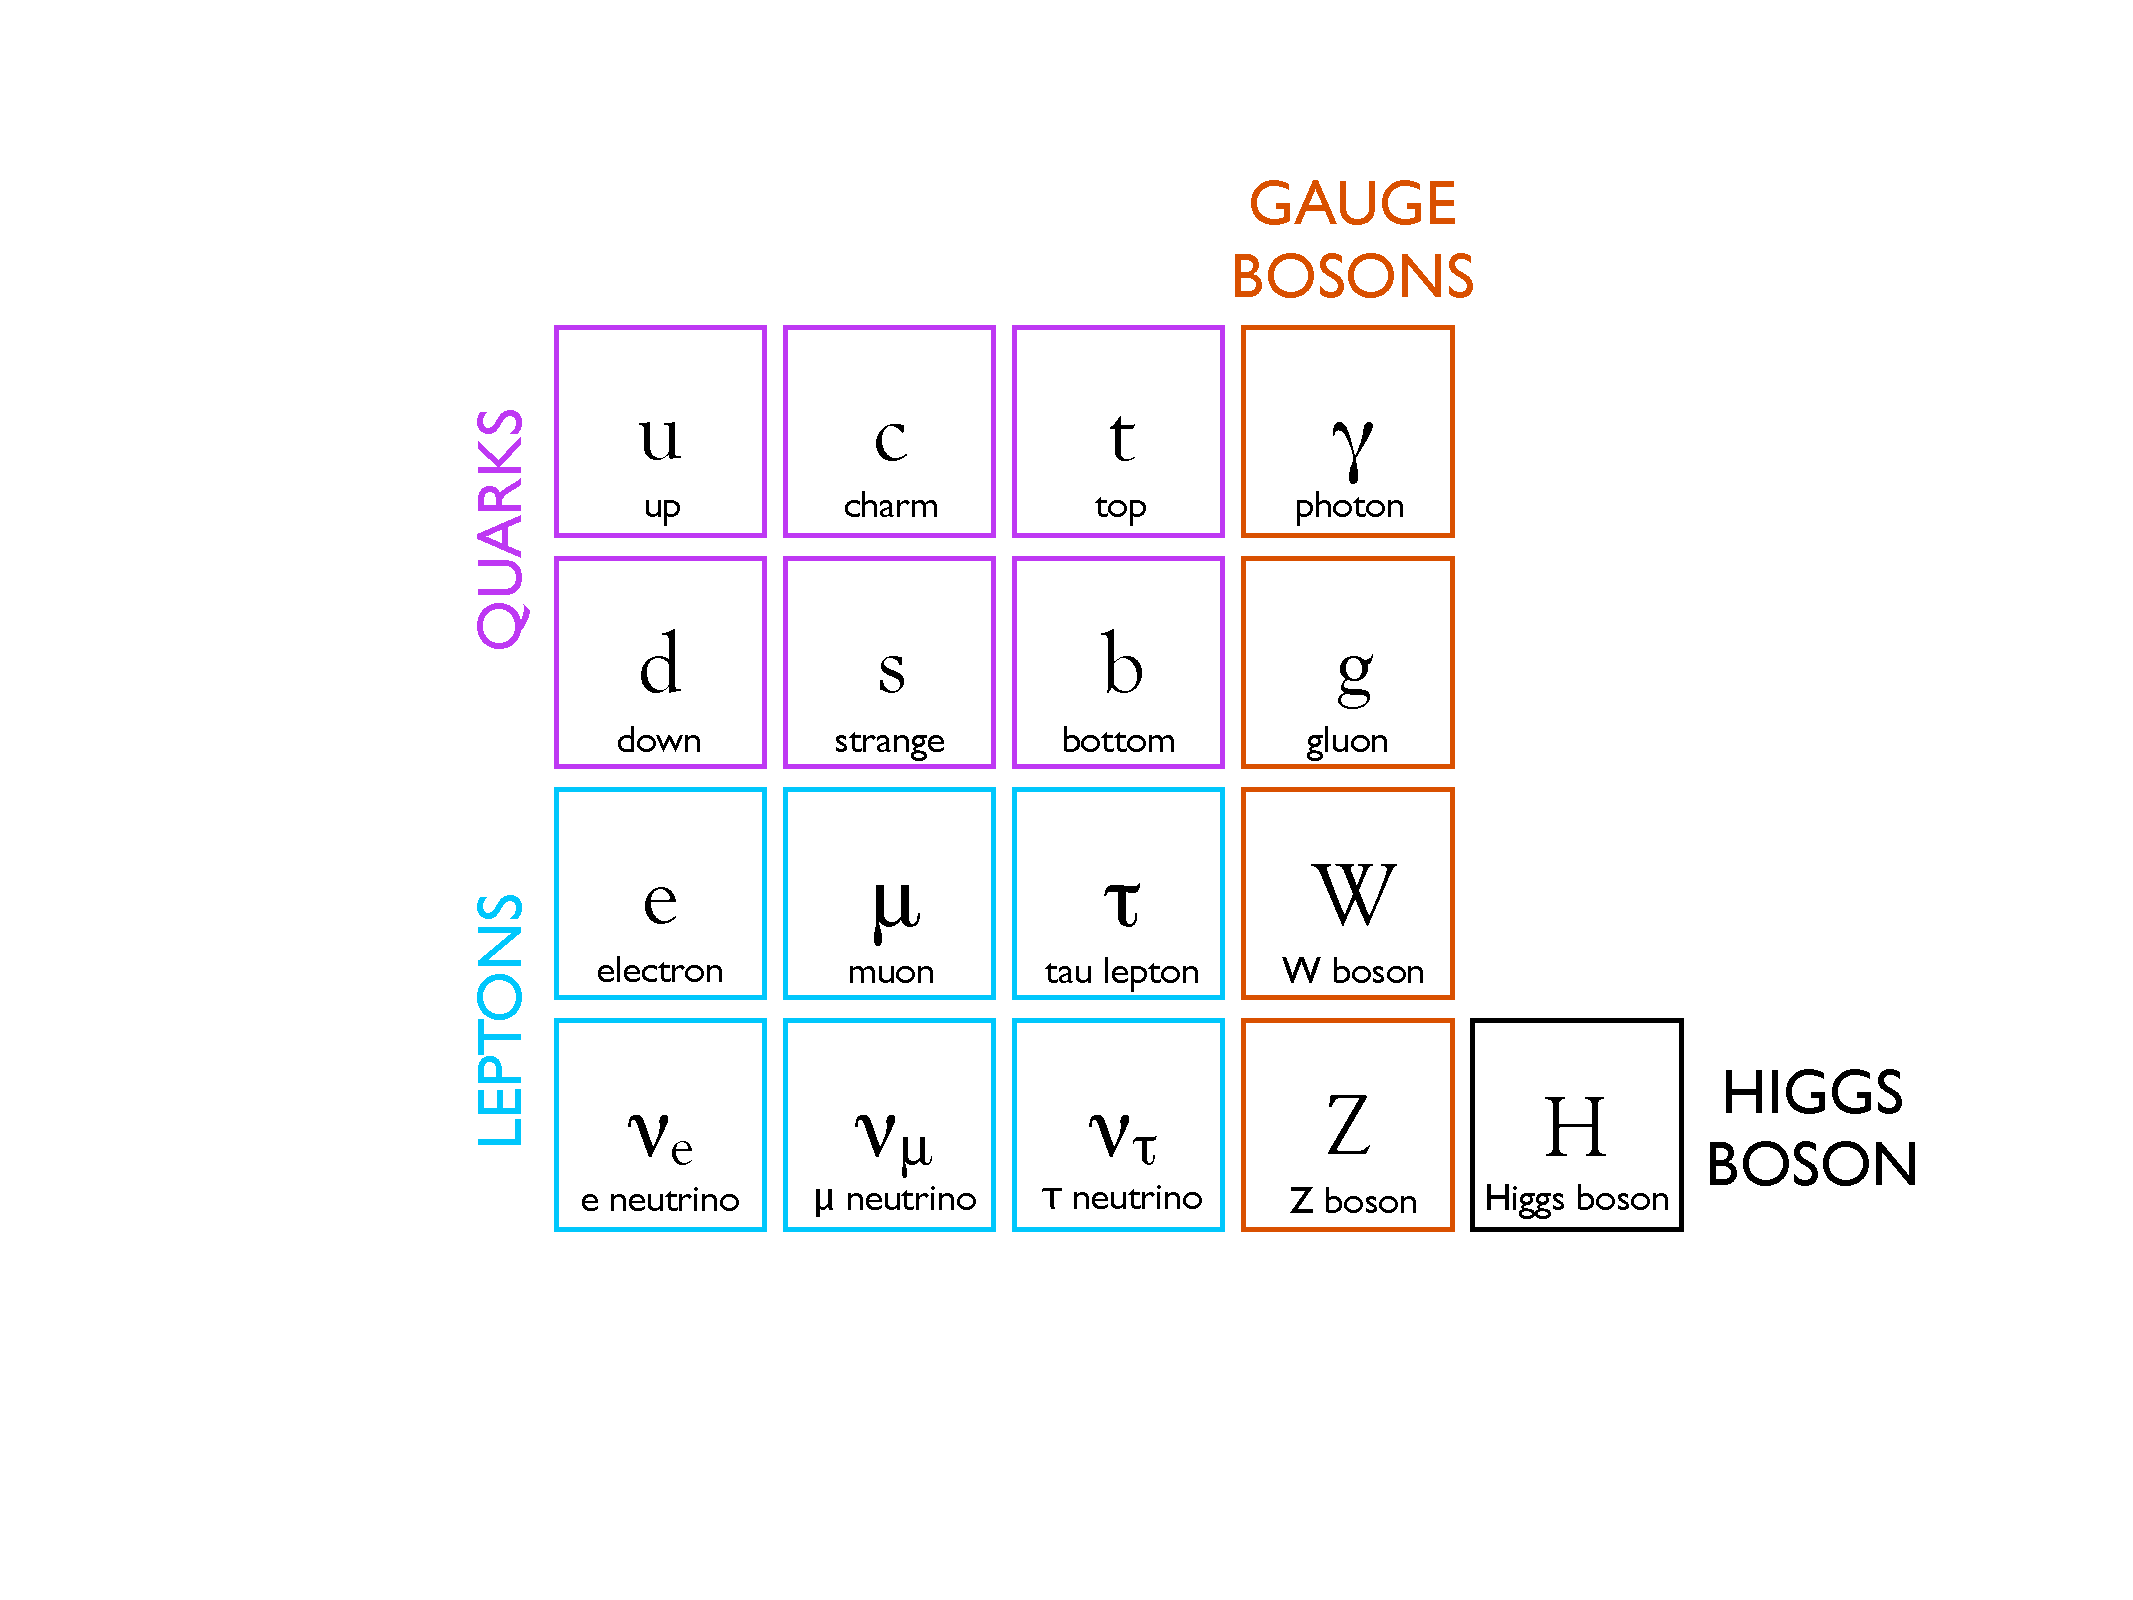
\includegraphics[width=0.6\textwidth]{figures/StandardModelTable}
      \caption{Standard Model particles.}
      \label{fig:StandardModelTable}
   \end{center}
\end{figure}

Leptons and quarks are fermions -- particles with half-integer spin whose dynamics obey the Dirac equation (see Equation~\ref{eq:Dirac}). Leptons fall into three generations called ``flavors", and have electric charge equal to integer multiples of the elementary charge $e =$ 1.6$\cdot$10$^{-19}$ C. The negatively charged leptons are the electron, the muon, and the tau (in increasing order of mass), and each is associated with an extremely light, neutral particle called a neutrino. Quarks have fractional multiples of the elementary electric charge and also possess another quantum property known as ``color" charge, whose implications will be explained shortly. There are three generations of quarks and a total of six different quark flavors (two per generation). For each quark and lepton, there exists an associated antiparticle.

The strong, electromagnetic, and weak interactions occur via the exchange of gauge bosons, which obey Bose-Einstein statistics and have spin 1. Each type of interaction involves the coupling of particles to the gauge field associated with that interaction. The theory describing the strong force is called quantum chromodynamics, or QCD. Quantum electrodynamics (QED) describes the electromagnetic force. At energies above $\mathcal{O}$(100) GeV, the electromagnetic interaction force unifies with the weak force, and the unified force is described by the electroweak theory.

Any particle with electric charge can participate in electromagnetic interactions, which are mediated by electrically neutral, massless photons. The strong force is mediated by gluons, which are colorless, electrically neutral, and massless; only quarks and gluons, which possess nonzero color charge, can participate in strong interactions. $W^{\pm}$ or $Z^{0}$ bosons are the carriers of the weak force, which is responsible for such processes as nuclear decays (they will hence be referred to as $W$ and $Z$, dropping the charge superscript unless it is necessary to mention their charges explicitly). W$^{+}$ and W$^{-}$ are one another's antiparticles, while Z and the photon are their own antiparticles. Unlike the gluon and photon, the $W$ and $Z$ bosons are massive.

The Standard Model belongs to the symmetry group SU(3)$\times$SU(2)$\times$U(1). The QCD Lagrangian $\mathcal{L}_{QCD}$ obeys the symmetry of the special unitary group SU(3), while the electroweak portion $\mathcal{L}_{EWK}$ obeys SU(2)$\times$U(1) symmetry.

In QCD, the eight generators of the SU(3) group give rise to eight gauge fields $G^{a}_{\mu}$, whose linear combinations correspond to gluons. The conserved quantity in QCD interactions is ``color" charge. An unusual feature of the strong force is that as the momentum transfer of the interaction increases, the strength of the interaction decreases. Thus, for high-energy interactions, the QCD coupling is small enough that perturbation theory can be applied to Feynman diagrams and quarks can be treated like free particles -- a property known as asymptotic freedom. The behaviour of the strong force at low energies, where QCD becomes non-perturbative, is still not well understood; one consequence of the low-energy scale behaviour of the strong force is color confinement, which means that quarks and antiquarks cannot be found free but can only exist in bound states called hadrons. The SU(3) invariance of hadronic wavefunctions restricts the only possible hadronic states to be SU(3) singlets -- i.e., states with a net zero color charge.

The quarks that make up a hadron, the gluons that bind them, and the fleeting quark-antiquark pairs that these gluons produce are collectively known as partons. The probability density for each parton to be found with a fraction $x$ of the total hadronic 4-momentum is described by its parton distribution function (PDF), which is determined by the strong interactions among the various partons in the hadron. In practice, PDFs cannot be calculated from theory alone because of the non-perturbative nature of QCD interactions at low energies; thus, they can only be measured experimentally~\cite{BettiniPhysics}.

Low-energy weak processes such as beta decays were first described by Fermi via a simple four-point interaction~\cite{0034-4885-42-12-001}. This, however, does not explain the experimental observation of parity violation in weak decays, and the predicted cross-section for weak decays blows up for high-energy processes ($q^2 >$ $\mathcal{O}$(100 GeV)$^2$) in the four-point interaction model. Electroweak theory developed in response to these issues; it predicted that weak interactions occur via parity-violating axial vector currents mediated by massive vector bosons~\cite{PerkinsPhysics}. In electroweak theory, the gauge fields $B_{\mu}$ (from the U(1) group) and \textbf{W}$^1$$_{\mu}$, \textbf{W}$^2$$_{\mu}$, and \textbf{W}$^3$$_{\mu}$ (from the SU(2) group) give rise to the electroweak gauge bosons~\cite{Bednyakov:2007pz}.

However, a problem arises from the fact that the Lagrangian for the electroweak gauge bosons can only be invariant under SU(2)$\times$U(1) transformations if the masses of its gauge bosons are zero. Although the photon is known to be massless, the $W$ and $Z$ bosons are clearly not. A prediction for the mass of the $W$ was first derived from measurements of the lifetime of the muon~\cite{ThomsonPhysics}, and the $W$ and the $Z$ were later both discovered in e$^{+}$e$^{-}$ collisions in the LEP experiment at CERN~\cite{Arnison:1983rp,Arnison:1983mk}.

\begin{figure}
   \begin{center}
      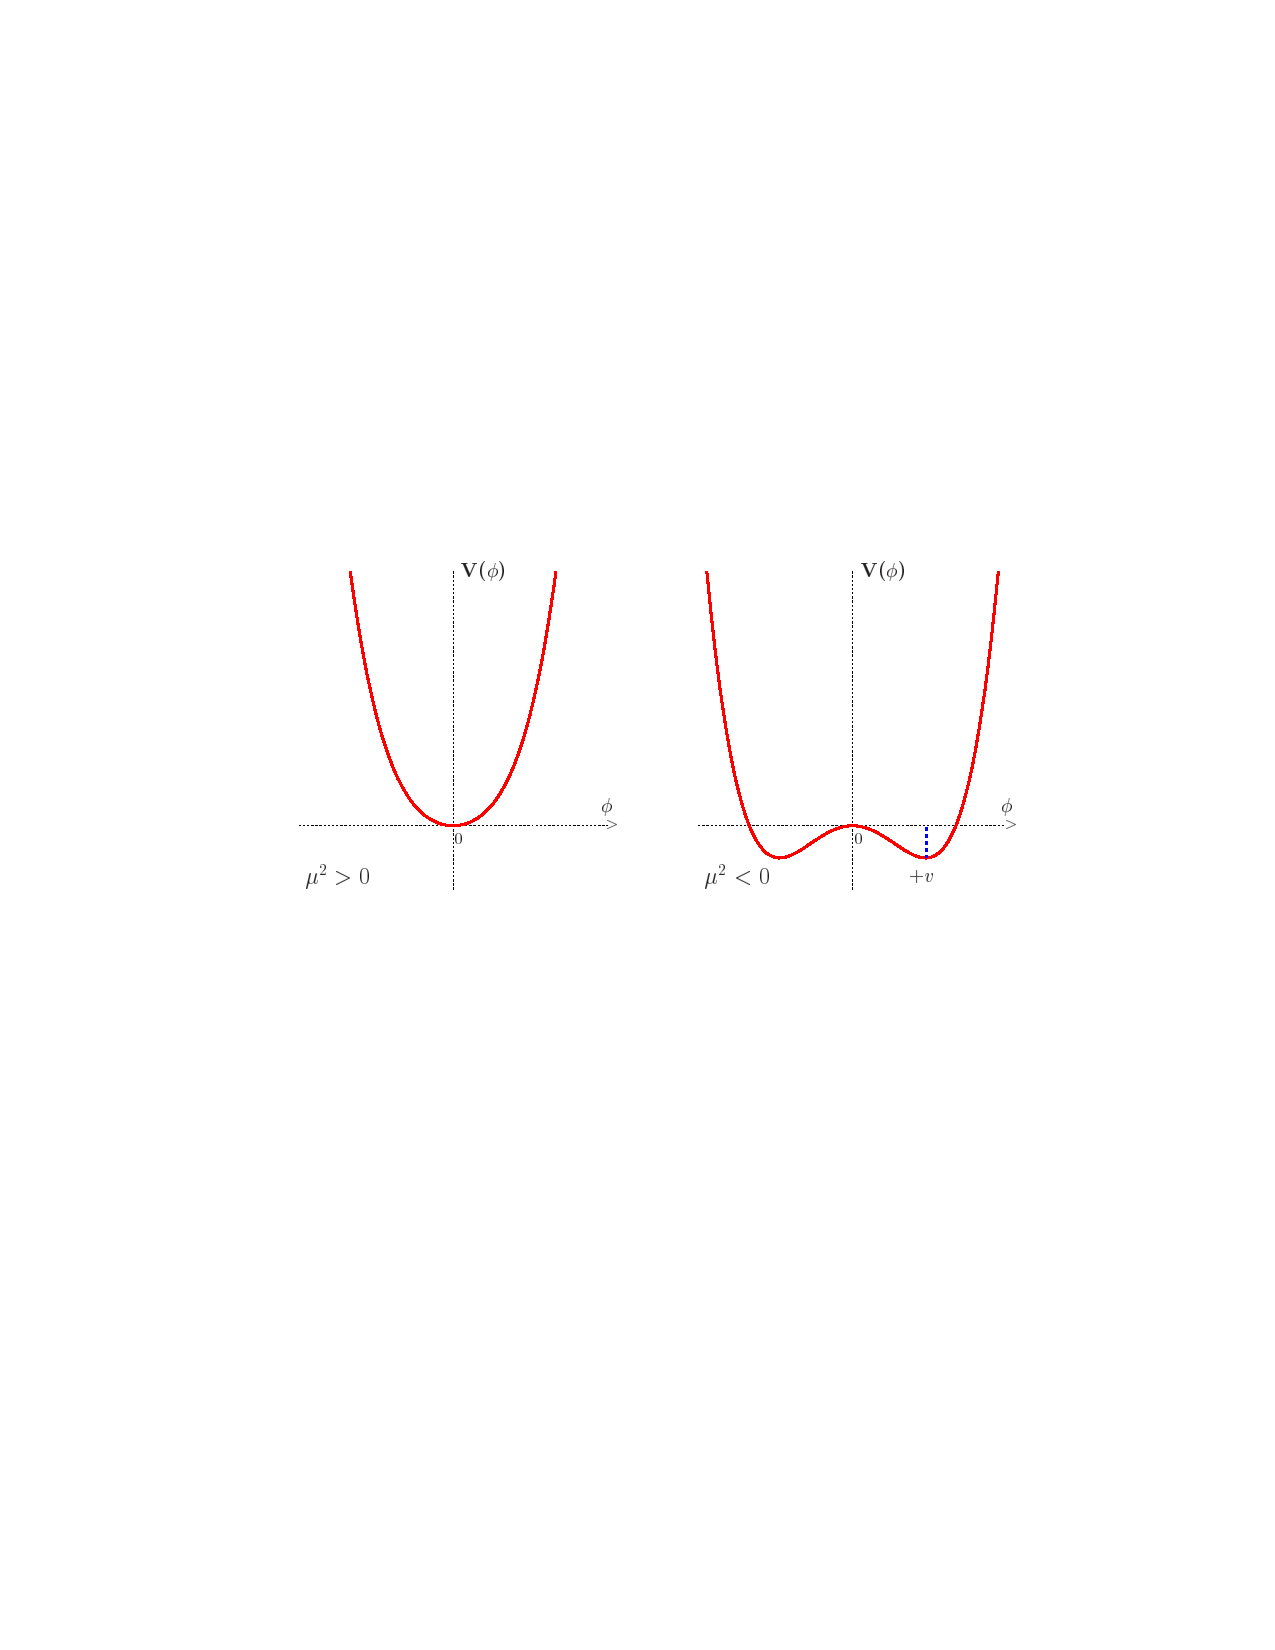
\includegraphics[width=0.6\textwidth]{figures/intro-Higgspotential}
      \caption{Illustration of spontaneous symmetry breaking in the case of a real scalar field $\phi$, with potential V($\phi$) $= \frac{1}{2}\mu^2\phi^2 + \frac{1}{4}\lambda\phi^4$. For $\mu^2 > 0$ (\cmsLeft), the potential has a minimum at zero and thus the vacuum expectation value of the field is zero. For $\mu^2 < 0$ (\cmsRight), the potential has two nonzero minima at $v = \pm\sqrt{-\frac{\mu^2}{\lambda}}$; in nature, the symmetry is broken by the choice of one of these two possible values for the vacuum expectation value of the field. Image copied from~\cite{Djouadi:2005gi}.}
      \label{fig:higgspotential}
   \end{center}
\end{figure}

The massive gauge boson paradox is resolved by the concepts of spontaneous symmetry breaking and the Higgs mechanism~\cite{ThomsonPhysics}. This involves the introduction of a complex scalar field whose vacuum expectation value is not zero but instead one of multiple nonzero minima of the scalar field potential. The choice of one of these vacuum expectation values breaks the symmetry of the scalar potential. This is illustrated in Figure~\ref{fig:higgspotential} for the simplified case of a real scalar potential with two local minima. When the Lagrangian of such a scalar field is expressed in terms of a perturbation of the field about its vacuum expectation value, this results in a mass term for the perturbation that corresponds to a scalar boson called a Goldstone boson.

To complete the picture, the spontaneous symmetry of the scalar field is embedded in the SU(2)$\times$U(1) symmetry, and this results in what is known as the Higgs mechanism. The simplest model requires two complex scalar fields. When the combined Lagrangian of the scalar fields and electroweak gauge fields is expressed as an expansion about the chosen vacuum expectation values of the scalar fields, one ends up with terms quadratic in the $B_{\mu}$, \textbf{W}$^1$$_{\mu}$, \textbf{W}$^2$$_{\mu}$, and \textbf{W}$^3$$_{\mu}$ fields, which are interpreted as mass terms. Via an appropriate gauge transformation, the Goldstone bosons resulting from the symmetry breaking disappear by being absorbed into the longitudinal degree of freedom of the \textbf{W}$^i$$_{\mu}$ fields, and the mixing of the four gauge fields results in the $W^{\pm}$ bosons, which are linear combinations of \textbf{W}$^1$$_{\mu}$ and \textbf{W}$^2$$_{\mu}$, and a $Z$ boson and a photon, both of which are linear combinations of \textbf{W}$^3$$_{\mu}$ and $B_{\mu}$. When this mixing is accounted for in the Lagrangian, the only mass terms that remain are the ones for the $W$ and $Z$ bosons, while the photon is massless. The existence of the Higgs field also generates the masses of the fermions via Yukawa interactions between fermions and the Higgs field in the electroweak Lagrangian.

\begin{figure}
   \begin{center}
      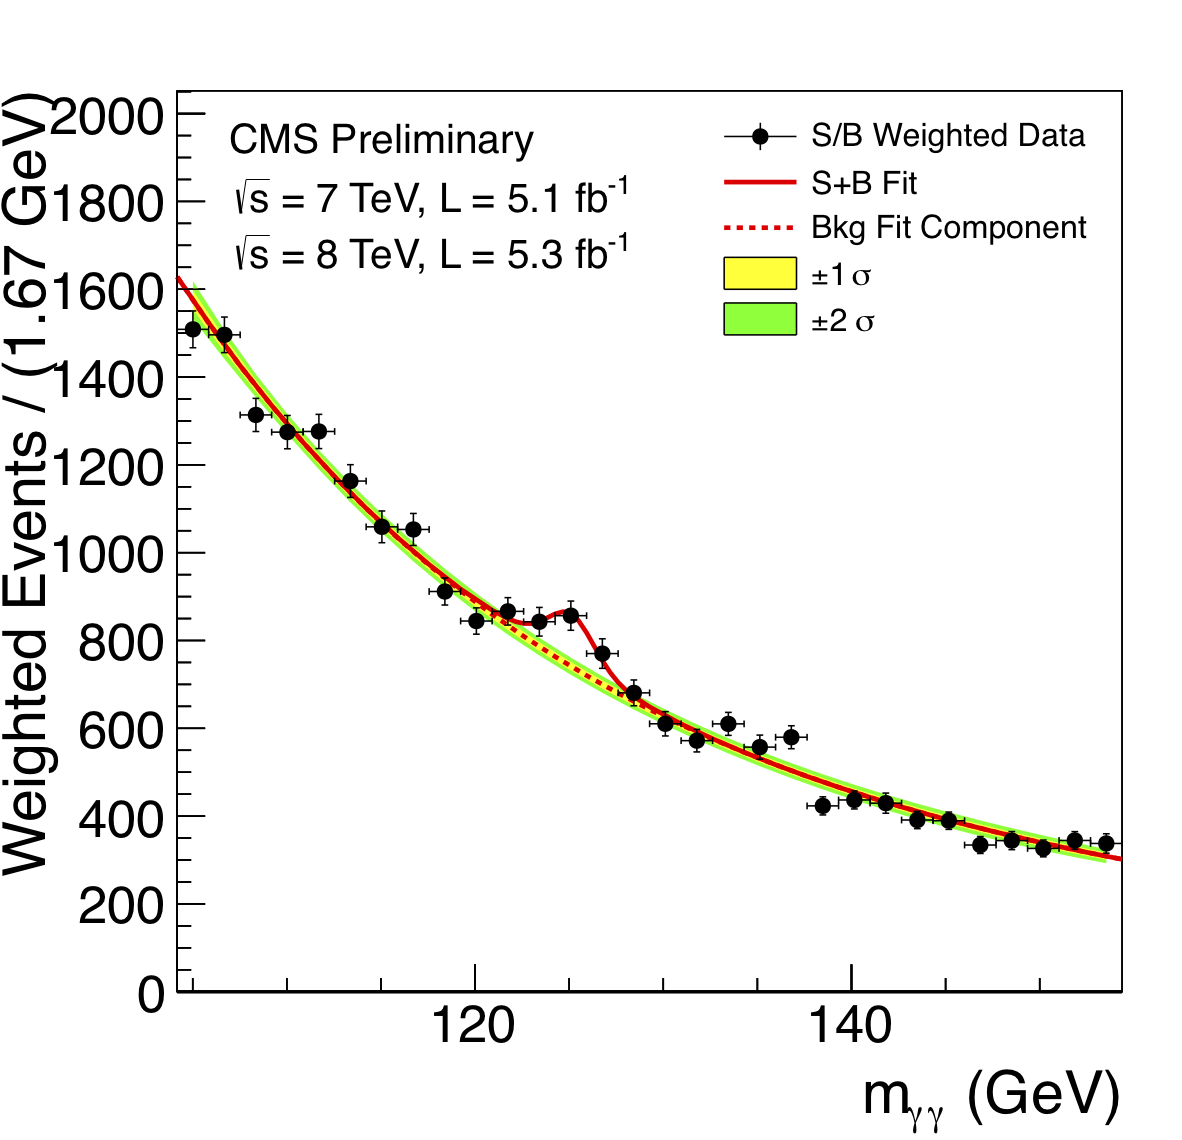
\includegraphics[width=0.6\textwidth]{figures/higgs-resonance}
      \caption{Observation of the Higgs resonance at 125 $\pm$0.4 (stat.) $\pm$0.5 (syst.) GeV in the diphoton spectrum at the CMS experiment~\cite{Chatrchyan:2012ufa}.}
      \label{fig:higgs-resonance}
   \end{center}
\end{figure}

Thus, the electroweak theory predicts the existence of a Higgs boson. This is the final particle is represented in Figure~\ref{fig:StandardModelTable}, the only known scalar particle in the Standard Model. The experimental search for this Higgs boson has carried on for decades after its existence was first predicted, and has finally culminated in its discovery at the LHC collider at CERN~\cite{Aad:2012tfa,Chatrchyan:2012ufa} (see Figure~\ref{fig:higgs-resonance}), providing a strong validation for this last major prediction of the Standard Model.

\section{Deficiencies of the Standard Model\label{sec:SMdeficiencies}}

Although the Standard Model has been successful in describing a wide range of experimental results, there is clear evidence that it is not complete. To name a few of its shortcomings~\cite{BettiniPhysics}:

\begin{itemize}
\item \textbf{Gravity: }The four fundamental forces are the strong force, electromagnetism, the weak force, and gravity. The Standard Model accounts for the first three, but the way in which gravity, which is $10^{32}$ times weaker than the weak force, factors into the Standard Model is still unknown.
\item \textbf{Neutrino oscillations: }The Standard Model treats neutrinos as massless particles. However, there is strong experimental evidence to the contrary. The observation of neutrino flavor oscillations, which cannot occur if neutrinos were massless, suggests that the observed electron, muon, and tau neutrino flavors are not in fact mass eigenstates -- rather, the observed neutrino flavor states are superpositions of mass eigenstates. What the mass eigenvalues are and why they are so small, are mysteries that remain to be resolved.
\item \textbf{Dark matter and energy: }Matter constitutes only about 30\% of the total mass-energy density of the universe; the remainder is comprised of ``dark matter" and ``dark energy", but their exact nature is unknown, and their presence is only deduced indirectly from their gravitational effects, since dark matter does not emit or absorb electromagnetic radiation. Thus, it is suspected that dark matter must be made up of some different type of particle not accounted for by the Standard Model.
\item \textbf{Grand unification: }The running coupling constants of the strong, electromagnetic, and weak interactions generally approach one another at increasingly higher energy scales. This suggests that these three fundamental interactions (and perhaps also gravity) might be manifestations of one unified field theory and thus may unify at some high energy scale; some theories predict this scale to be on the order of 10$^{16}$ GeV.
\item \textbf{The hierarchy problem: }The Standard Model predicts that the mass of the Higgs boson receives loop corrections from leptons, quarks, and whatever other particles may couple to the Higgs. As a result, the Higgs mass would be expected to receive corrections up to the order of the Planck scale ($\mathcal{O}$(10$^{19}$ GeV)) at which gravity becomes significant and the Standard Model of physics no longer holds. The fact that the magnitude of the actual Higgs mass is so much lower than those of the predicted corrections is surprising, as it implies that there must be some mechanism by which these corrections are cancelled. This constitutes what is known as the hierarchy problem of the Standard Model.
\end{itemize}

These deficiencies indicate that there is physics beyond the Standard Model, and that more elements are needed to provide an accurate description of nature.

\section{Supersymmetry}

One theory that has been proposed to address the hierarchy problem is that there exists a certain symmetry -- called supersymmetry -- that relates fermions to bosons~\cite{Martin:1997ns}. For each fermion, there would exist a corresponding bosonic parter particle, and likewise for each boson there would exist a fermionic partner; such partner particles are referred to as superpartners. Under a supersymmetric transformation, a fermion turns into its superpartner and vice versa. Thus, for each loop correction to the Higgs mass, there would be another loop correction from the supersymmetric partner particle; since fermionic loops have a sign opposite that of bosonic loops, the loop corrections would cancel neatly.

As supersymmetry posits a superpartner for every Standard Model particle, it is of great interest to look for experimental evidence of these superpartners, none of which have yet been observed in nature. The question is where to look, since there is nothing that specifies the masses of supersymmetric particles or the other numerous other free parameters in the theory of supersymmetry. These free parameters must be constrained by experimental measurements.

The masses of supersymmetric particles must be different from the masses of their Standard Model counterparts, otherwise the supersymmetric particles would have been observed already. In order to have this inequality in masses, supersymmetry must be a broken symmetry. There are many models for the mechanism of supersymmetry breaking; but in general, in order to achieve the stabilization of the Higgs mass, the symmetry breaking scale is expected to be on the order of 1-10 TeV~\cite{Aitchison:2005cf}. Since the mass splittings between Standard Model particles and their superpartners are determined by the supersymmetry breaking parameters, the masses of the lightest supersymmetric particles are  expected to be around the same scale of 1-10 TeV as well. Thus, if supersymmetric particles exist, it could be possible to discover them in high-energy collider experiments such as the LHC at CERN.

The simplest model incorporating supersymmetry into the Standard Model is the Minimal Supersymmetric Standard Model (MSSM)~\cite{Martin:1997ns}. The details will not be covered here, but the Higgs sector consists of two chiral Higgs supermultiplets $H_u$ and $H_d$, of which the former couples to up-type quarks and the latter couples to down-type quarks and charged leptons. The superpotential $W_{MSSM}$ of the MSSM, which defines the most general non-gauge interactions for the superfields, is:

\begin{equation}
W_{MSSM} = \bar{u}y_{u}QH_{u} - \bar{d}y_{d}QH_{d} - \bar{e}y_{e}LH_{d} + \bar{\mu}H_{u}H_{d}
\label{eq:WMSSM}
\end{equation}

While the MSSM does provide a cancellation of large corrections to the Higgs mass, it comes with deficiencies of its own. One problem, called the $\mu$-problem, stems from the fact that the $\mu$ parameter in Equation~\ref{eq:WMSSM}, which must have the dimension of mass, must be of the order of magnitude of the electroweak scale in order to provide the Higgs doublets with vacuum expectation values on the order of the electroweak scale. However, its magnitude is expected to be more naturally close to the Planck scale, which is significantly larger. Fine-tuning its magnitude to that of the electroweak scale thus seems arbitrary and without theoretical motivation.

The $\mu$-problem is avoided in the Next-to-Minimal Supersymmetric Standard Model (NMSSM)~\cite{Maniatis:2009re}, which extends the Higgs sector of the MSSM by a scalar Higgs singlet field S and ultimately predicts a total of seven Higgs bosons -- a pair of charged ones, three neutral scalars, and two neutral pseudoscalars. The NMSSM superpotential is:

\begin{equation}
W_{NMSSM} = W_{MSSM} + \lambda SH_{u}H_{d} + \frac{1}{3}\kappa S^3 + \frac{1}{2}\mu_{s}S^2
\label{eq:WNMSSM}
\end{equation}

The coupling of the singlet field $S$ to the doublet fields naturally generates an effective $\mu$ term via the expectation value of $S$. Thus, $\mu = \lambda$$<S>$, with the desired magnitude near the electroweak scale. The fact that the NMSSM circumvents the $\mu$-problem makes it of great interest to study. The new physics search presented in this dissertation is a probe into the Higgs sector of the NMSSM.
\chapter{Experiment description\label{sec:experiment}}

\section{Large Hadron Collider\label{sec:lhc}}

The Large Hadron Collider (see~\cite{1748-0221-3-08-S08001} for a detailed description) is a circular accelerator and collider of high-energy particles, straddling the French-Swiss border near Geneva, Switzerland. Constructed between 1998 and 2008, the accelerator consists of 2 rings for counter-circulating proton or ion beams, 27 km in circumference and located at depths as low as 175 m underground in the tunnel previously occupied by the LEP collider ring. Superconducting magnets, composed of NbTi Rutherford conductors cooled to temperatures below 2 K with superfluid helium, generate magnetic fields above 8 T and serve to steer and focus the particle beams (either protons or lead ions) in their trajectory through the accelerator rings.

Protons, derived by ionizing hydrogen gas, are accelerated first via a linear accelerator to an energy of 50 MeV and injected into the Proton Synchrotron Booster, which accelerates them to 1.4 GeV. From there, they are injected into the Proton Synchrotron, which accelerates them further to 25 GeV, and then into the Super Proton Synchrotron, which brings them to an energy of 450 GeV before finally injecting them into the LHC ring, in which they are accelerated to the desired center-of-mass energy for collisions. The LHC has been designed to collide protons at a maximum center-of-mass energy of 14 TeV. During its first run, it operated at center-of-mass energy 7 TeV from 2010-2012, and then at 8 TeV from 2012-2013. After a long shutdown for planned repairs and maintenance, the LHC was restarted in 2015, operating at 13 TeV, with the intention of eventually increasing to 14 TeV.

The LHC is home to several experiments -- the general-purpose high-luminosity detectors ATLAS (A Toroidal LHC Apparatus) and CMS (Compact Muon Solenoid), low-luminosity detectors LHCb (focusing on B physics) and TOTEM (focusing on elastic proton scattering), and the heavy-ion detector ALICE. At each detector, the proton beams are focused together by quadrupole magnets at an interaction point, where they collide, and the particles produced in these collisions are detected and recorded by the detector system. The rest of this chapter will focus on the CMS experiment, where the research described in this thesis was conducted.

\section{Compact Muon Solenoid\label{sec:cms}}

The Compact Muon Solenoid (CMS) detector is a hermetic general-purpose detector at the LHC, gathering data from the collision of proton-proton and heavy ion beams to study a wide range of physics processes. This experiment is characterized by a powerful superconducting solenoid magnet that produces a 4 T magnetic field; the paths of charged particles are bent by the magnetic field, allowing their momenta to be accurately reconstructed from their trajectories. Quadrupole magnets bend the two proton beams passing through the LHC ring to intersect and collide at the interaction point (IP) in the center of the CMS detector, and the particles produced in the collision pass through and are recorded by the layered system of cylindrical subdetectors that comprise the CMS detector. At the center of the ensemble is a silicon tracker subdetector for reconstructing accurately the momenta of charged particles. Encircling it is the electromagnetic calorimeter (ECAL), a homogenous calorimeter that uses scintillating lead tungstate crystals to reconstruct electrons and photons with high energy resolution. Outside the electromagnetic calorimeter is the hadron calorimeter (HCAL), a sampling calorimeter with alternating layers of brass and scintillator that measures the energy deposited in hadronic showers. The solenoid magnet is located outside the hadronic calorimeter, together with an iron yoke system that provides a return flux for the magnetic field. The outermost layer of the CMS detector is the muon tracking system for identifying and reconstructing the trajectories of muons. The solenoid magnet and the various subdetectors of CMS will be described in more detail in the rest of this chapter, followed by considerations regarding the mechanisms for data collection by CMS. A more complete description of the detector can be found at~\cite{1748-0221-3-08-S08004}; unless otherwise specified, all information in this chapter is derived from this source.

\subsection{Magnet\label{sec:cms-magnet}}
% solenoid, yoke, cryogenics, vacuum system

The superconducting solenoid magnet of CMS encloses the tracker detector, ECAL, and part of the HCAL inside a cylindrical bore 6.3 m in diameter and 12.5 m long, weighing 220 tonnes. The solenoid is composed of a 4-layer winding of coils made of NbTi, which is mechanically reinforced by being mixed with an aluminium alloy, an innovative method that makes the coils serve both as conductors and as their own self-stabilizing structural support. At full current, the solenoid carries 19.14 kA, producing a nearly uniform 4 T magnetic field through the volume enclosed by the bore, containing 2.6 GJ of stored energy. The magnetic flux is returned through an iron yoke, consisting of a system of barrel wheels and endcap disks arranged outside the volume of the solenoid in a cylindrical pattern and interleaved with the muon tracking system; the yoke consists of 5 iron rings, each 2.536 m wide in the z direction, positioned at z = -5.342 m, -2.686 m, 0 m, +2.686 m, and +5.342 m (rings number -2, -1, 0, 1, and 2 respectively).

\subsection{Tracker\label{sec:cms-tracker}}

5.8 m in length along the z axis and 2.5 m in diameter, the tracker detector is the innermost layer of the CMS detector system. Its purpose is to reconstruct the paths and momenta of charged particles with transverse momentum 1 GeV and upwards, and to provide good impact parameter resolution for accurately reconstructing the positions of secondary vertices, which are displaced from the point of collision and generally are a characteristic signature of long-lived particles such as those from heavy-flavour processes. Since the tracker detector receives higher irradiation than any other part of the detector due to its proximity to the beam line and the interaction point (IP), the tracker detector has been designed to perform in a high-flux environment, with thousands of particles passing through its volume every 25 ns when the LHC is running at its design luminosity. Thus, the tracker has been designed with these challenges in mind in order to yield good position and time resolution.

The tracker detector is composed of two subdetectors. The one closest to the beam line is the pixel detector; its sensors are 100 $\mu$m x 150 $\mu$m pixels, which receive an occupancy on the order of $10^{-4}$ per pixel per bunch crossing. The second and larger subdetector is the silicon strip tracker, whose sensors are silicon strips; since it is located at larger radii than the pixel detector, the fluence of particles that reach it is lower and thus the granularity of the silicon strips can be considerably lower than that of the pixel detector, with strip areas ranging from 10 cm x 80 $\mu$m at intermediate radii for the inner strip tracker (20 $<$ r $<$ 55 cm) and 25 cm x 180 $\mu$m for the outer strip tracker (55 $<$ r $<$ 110 cm), resulting in an occupancy of about 2-3\% for the inner tracker and 1\% for the outer tracker. In total, the CMS tracker detector is comprised of 200 $m^{2}$ of active silicon sensors, providing a coverage of up to $\abs{\eta}$ $<$ 2.5.

The support structures that hold the sensors in position are designed to minimize the amount of material used, since energy loss via multiple scattering and extraneous particles produced by nuclear interactions, gamma conversions, and bremsstrahlung in the supporting material can all interfere with tracking efficiency. Because of the high particle fluence passing through the tracker volume during operation, radiation-hard sensors and electronics are required to withstand the radiation dosage; also, an efficient system system of cooling tubes carrying chilled liquid $C_{6}F_{14}$ pervades the tracker volume, keeping it at or below -10 C during operation, thus minimizing radiation damage to the sensors caused either by direct irradiation or by the annealing of radiation-induced defects in the silicon crystal structure through thermal agitation.

\subsubsection{Pixel detector\label{sec:cms-pixel}}
% barrel and disks, design of sensors, electronics, readout

The pixel detector is the innermost layer of the tracker detector, with three concentric cylindrical barrel layers complemented by two endcap disks on either side of the interaction point. The barrel layers are located at radii 4.4, 7.3, and 10.2 cm from the beam line, extending out to 2.9 m from the interaction point in the $\pm$z directions. Two endcap disks are located at z $=$ $\pm$34.5 cm and $\pm$46.5 cm, with inner radius 6 cm and outer radius 15 cm. Both the barrel cylinders and endcap disks are split in halves along the y axis for ease of extraction and access. Each sensor has an area of 100 $\mu$m x 150 $\mu$m; the nearly square design is intended to provide good cluster size and hit resolution in both r$\phi$ and z for the barrel and r$\phi$ and r for the endcaps, as both of these coordinates are needed for measuring track impact parameters.

In the barrel, the sensors are arranged 2 x 8 on rectangular modules (or 1 x 8 along the edges of the half-cylinders). In each endcap half-disk, 12 trapezoidal support structures called blades hold the sensors, which come in arrangements of five different plaquette sizes (1 x 2, 2 x 3, 2 x 4, 1 x 5, and 2 x 5) in order to achieve full coverage of the wedge-shaped area of the blade. Altogether, the pixel detector covers a pseudorapidity range of $\abs{\eta}$ $<$ 2.5.

The pixel sensors consist of 52 x 80 high-dose $n$-type pixels implanted in a high-resistance $n$-type substrate of 320 $\mu$m thickness on a sensor plate. Each pixel is bump-bonded onto a readout chip (ROC) connected to the sensor plate. The ROC collects and amplifies the analog signals from the pixels, storing them in a buffer until the arrival of the appropriate readout control and clock signals causes it to pass the sensor signal on to the readout system.
 
When a charged particle passes through a silicon sensor, it induces charge carriers in the n-doped silicon substrate; traveling towards the pixels to be collected, electrons undergo a signficant Lorentz drift (roughly 32$^{\circ}$) due to the 4 T magnetic field along the z axis through the tracker volume, and thus the signal current ends up being spread over adjacent pixels. Interpolation between signals from multiple neighbouring pixels can be used to improve hit resolution. In the barrel, the normal direction of the pixel cells points along the radial direction, perpendicular to the magnetic field, so the Lorentz drift is along the r$\phi$ direction. To induce charge sharing in the pixel endcaps, whose normal points along the magnetic field axis, the blades are rotated at a 20$^{\circ}$ angle about their radial axis in a turbine-like geometry.

\subsubsection{Silicon strip detector\label{sec:cms-strips}}
% barrel and disks, design of sensors, electronics, readout

Outside the pixel detector, at radius 20 cm to 116 cm about the beam line and extending 118 cm in the +z and -z directions, lies the silicon strip detector. It is composed of 3 main subsystems: the tracker inner barrel and disks (TIB and TID), the tracker outer barrel (TOB), and the tracker endcaps (TEC). To optimize coverage, the silicon microstrip sensors in any given barrel layer or endcap disk are positioned to partially overlap with one another, thus resulting in a nonzero pitch with respect to the surface to which they are attached.

The TIB consists of 4 barrel layers 140.0 cm in length, with radii of 255.0 mm, 339.0 mm, 418.5 mm, and 498.0 mm, altogether providing up to 4 r-$\phi$ measurements per particle trajectory. The sensors are silicon microstrips with a thickness of 320 $\mu$m, lying parallel to the beam axis, with a pitch of 80 $\mu$m on the inner two layers and 120 $\mu$m on the outer two layers, yielding a single-point resolution of 23 $\mu$m for the inner two layers and 35 $\mu$m for the outer two layers. The TID is comprised of six endcap disks, three at each end of the TIB between $\pm$80.0 cm and $\pm$90.0 cm on the z axis; each disk consists of three support rings from radius 200 $\mu$m to 500 $\mu$m. Silicon microstrips, similar to the ones used in the barrel, lie radially on the disks, with a pitch varying from 100 $\mu$m to 141 $\mu$m. While the pixel detector is split down the y axis into half-cylinders for ease of installation, access, and independent testing, the TIB and TID are split into half-shells along the x axis for similar reasons. Two carbon-fibre service cylinders are coupled to the $\pm$z ends of the TIB, providing a route to the TIB shells for service cables originating from a service distribution disk called a margherita, and also housing the TID.

The TOB surrounds the TIB with 6 barrel layers, reaching to an outer radius of 116 cm and spanning 118 cm in the $\pm$z directions. The silicon microstrip sensors here are 500 $\mu$m thick and have a pitch of 183 $\mu$m in the inner four layers and 122 $\mu$m in the outer two layers, yielding a single-point resolution of 53 $\mu$m and 35 $\mu$m respectively in those layers. On either end of the TOB, the TEC extends radially from 220 mm to 1135 mm and in the $\pm$z direction from $\pm$1240 mm to $\pm$2800 mm; each side consists of an assembly of 9 disks with up to 7 rings bearing silicon microstrip sensors, plus 2 extra disks that serve as front-back termination. The microstrip sensors used here have a thickness of 320 $\mu$m in the four rings closest to the TOB and 500 $\mu$m in the remaining outer rings, with a pitch varying from 97 to 184 $\mu$m.

The silicon microstrip sensors used have a single-sided p-on-n design. Signal currents are amplified and stored by a custom integrated circuit called an APV25 before being transmitted via optical fibers through the readout system for digitization and storage.

\subsection{Electromagnetic calorimeter\label{sec:cms-ecal}}
% crystals, photodetectors, readout, preshower

The electromagnetic calorimeter (ECAL) is a hermetic homogeneous calorimeter made up of lead tungstate (PbWO$_4$) crystals; similar to the inner tracking system, it is composed of a cylindrical barrel system (with a total of 61,200 crystals) and an endcap system (one endcap disk on each side of the barrel, with 7324 crystals per disk). When electrons or photons pass through the ECAL, the resulting electromagnetic showers that they generate excite the scintillator atoms, causing them to emit blue-green scintillation light (up to 420-430 nm in wavelength) that is collected, amplified, and read out by photodetectors glued to the ends of the crystals. High granularity is needed for good energy resolution in the ECAL; the choice of PbWO$_4$, with a density of 8.28 g/cm$^3$, a radiation length of 0.89 cm, and a Moliere radius of 2.2 cm, allows for compact, granular crystals that can resist radiation damage under the high particle fluences that the detector is subjected to throughout its operation. As the number of scintillation photons produced by the crystals and the amplification provided by the photodiodes both tend to decrease with increasing temperature, the temperature of the ECAL detector needs to be maintained at a steady operating temperature during its operation; this is done by a cooling system that uses water as a coolant, maintaining the ECAL at a stable temperature of 18$^{\circ}$ C with an uncertainty of $\pm$0.05$^{\circ}$ C.

The barrel extends from an inner radius of 1.29 m to an outer radius of 1.77 m. In the barrel, the detector granularity is 360-fold in $\phi$ and 170-fold in $\eta$. The crystals have a truncated pyramidal shape that varies with their position in $\eta$, with a cross-sectional area of approximately 22x22 mm$^2$ at the front face (closest to the beam line) and 26x26 mm$^2$ at the rear face, and a length of 230 mm (corresponding to 25.8 radiation lengths). Groups of 2x5 barrel modules are referred to as sub-modules, encased within a 0.1-mm thick wall consisting of an aluminium layer facing the crystal, followed by two layers of glass fibre-epoxy resin. Submodules are grouped together into larger groups called modules containing 400 or 500 crystals, whose shape depends on the position in $\eta$ of the module. Four modules form a supermodule, and 18 supermodules form half a barrel.

On either side of the barrel, the ECAL endcaps cover the pseudorapidity range 1.479 $<$ $\abs{\eta}$ $<$ 3.0. Endcap crystals have a truncated pyramidal shape similar to barrel crystals, with a front face cross-sectional area of about 28.62x28.62 mm$^2$ and a rear face cross-sectional area of 30z30 mm$^2$, and a length of 220 mm (24.7 radiation lengths). They are arranged in groups of 5x5 known as supercrystals, enclosed in a carbon-fibre alveolar wall. Each half of an endcap disk, called a Dee, is composed of 138 full supercrystals and 18 partial supercrystals.

Sandwiched between the barrel and each endcap disk is a disk-shaped sampling calorimeter with a thickness of 20 cm; these two disks make up the preshower detector. Its main purposes are neutral pion identification and rejection in the fiducial region 1.653 $<$ $\abs{\eta}$ $<$ 2.6, identify electrons against the background of minimum ionizing particles, and improve the position resolution of electrons and photons in the ECAL. The preshower is two layers thick; each layer consists of a layer of lead radiators for initiating electromagnetic showers, followed by a layer of silicon strip sensors for detecting the showers.

To take advantage of total internal reflection for the collection of scintillation light, all the ECAL crystals have been precisely polished during production. The crystals have a truncated pyramidal shape, which would tend to cause nonuniform light collection along the length of barrel crystals; thus, in the barrel crystals, one crystal face is left unpolished to compensate for this effect. This technique is not used in the endcaps because the endcap crystal faces are nearly parallel to one another, thus resulting in more uniform light collection. The different magnetic field configuration and particle flux in the barrel and endcaps led to different choices of photodetectors for those two systems: avalanche photodiodes (APDs) for the barrel and vacuum phototriodes (VPTs) in the endcaps. At 18$^{\circ}$ C, approximately 4.5 photoelectrons per MeV of deposited energy are collected by both APDs and VPTs. For electron or photon energies below 500 GeV, the ECAL energy resolution can be estimated as follows:

\begin{equation}
(\frac{\sigma}{E})^2 = (\frac{S}{\sqrt{E}})^2 + (\frac{N}{E})^2 + C^2
\end{equation}

In this equation, S is the stochastic term, N is the noise term, and C is the constant term. The stochastic term S comes from stochastic fluctuations in electromagnetic shower containment, a photostatistics contribution of 2.1\% coming from the uncertainty on the number of primary photoelectrons produced per MeV of deposited energy, and fluctuations in the energy deposited in the preshower absorber. The term N accounts for noise due to electronics, the signal digitization process, and energy deposited by pileup particles. Finally, the constant term C covers various sources of systematic error including the nonuniformity of light collection due to crystal shape, intercalibration errors, and leakage of energy from the back of the crystal.

\subsection{Hadronic calorimeter\label{sec:cms-hcal}}
% HB, HE, HO, HF -- scintillator, absorber, readout

Surrounding the ECAL is the hadronic calorimeter (HCAL), a sampling calorimeter extending radially from 1.77 m to 2.95 m from the beam line. Its main goals are to measure the energy deposited by hadronic jets in each event, and to measure indirectly the missing energy due to neutrinos and any potential exotic particles. The HCAL is split up into four subsystems, of which the innermost are the HCAL barrel and endcaps. To provide enough calorimeter material to absorb hadronic showers for jet and missing energy measurement while respecting the spatial constraints from ECAL within and the superconducting solenoid without, the barrel and endcaps are supplemented respectively by the outer calorimeter outside the solenoid and the forward calorimeters outside the muon endcaps. Altogether, these four subsystems provide coverage up to $\abs{\eta}$ $<$ 5.2.

The barrel system (HB) covers up to $\abs{\eta}$ $<$ 1.3. It is subdivided transversally into two half-barrels, each of which consists of 18 identical wedges (making a total of 36 HB wedges). The wedges are subdivided into 4 azimuthal sectors staggered for optimum coverage, and they hold the absorber plates and scintillator material. The HB absorber is made up of an innermost 40-mm-thick steel front plate, eight 50.5-mm-thick brass plates, six 56.5-mm brass plates, and an outermost 75-mm-thick steel back plate. Passing hadrons interact with the nuclei of the absorber, producing hadronic showers of quarks and gluons. The energy in these showers is deposited in and measured by 17 layers of scintillator material that are interspersed between the absorber plates; layers in azimuthal sectors 1 and 4 fit into slots in the edges of a wedge, while layers in azimuthal sectors 2 and 3 fit into slots in the middle of a wedge. Besides the division into 18 sectors in $\phi$, the scintillator material is also split into 16 sectors in $\eta$, resulting in a granularity of (0.087, 0.087) in ($\eta$, $\phi$).

The smallest scintillator unit is called a tile; tiles in layer 0 are made of Bicron BC408 and primarily serve to sample hadronic showers that develop between the HB and the ECAL barrel, while tiles in layers 1-16 are made of of Kuraray SCSN81 plastic scintillator. Tiles in a given azimuthal layer are grouped into units called trays for ease of assembly, access, and individual testing; each barrel layer contains a total of 108 trays. The scintillation light produced in each tile is collected by a Kuraray Y-11 wavelength-shifting (WLS) fibre. Each WLS fibre is spliced to a clear Kuraray double-clad fibre that serves all the tiles in the tray and delivers the collected light to an optical decoding unit, which arranges the clear fibres into readout towers and transmits their signals to a hybrid photodiode (HPD) for amplification and readout. Multipixel HPD's were chosen because of the wider range of wavelengths that they can detect and their low sensitivity to magnetic fields; those used in the HB, HE, and HO have a gain of ~2000.

The endcap system (HE) disks on either side of the HB are mounted onto the iron yoke of the muon endcap system and span the pseudorapidity range 1.3 $<$ $\abs{\eta}$ $<$ 3. The HE disks are subdivided azimuthally into 36 identical wedges and 18 layers, with 79-mm-thick brass absorber plates. The active material in the trapezoidal scintillator tiles is Bicron BC408 for layer 0 and SCSN81 for the remaining 17 layers. The HE contains a total of 20916 tiles, arranged into 1368 trays, with a granularity of (0.087, 0.087) in ($\eta$, $\phi$) for $\abs{\eta}$ <$\textless$1.6 and (0.087, 0.087) for $\abs{\eta}$ $\geq$ 1.6. The collection of scintillation light by WLS fibres and the transmission of the collected signal from tray to HPD for readout is similar to the design of the HB.

The cylindrical outer calorimeter (HO) is located outside the solenoid, taking advantage of the solenoid coil as an additional sampling layer for late-starting hadronic showers. The HO layers are mounted within the iron yoke that returns the magnetic field of the solenoid; they are the first sensitive layer in each of the 5 rings of the yoke. Ring 0 of the yoke has two layers of HO scintillators on either side of a 19.5-cm thick iron barrel at radii 3.82 and 4.07 m, while the other four rings have one layer of HO scintillator at radius 4.07 m. Each layer of the HO is divided into 12 sectors in $\phi$, each separated by the dead space of 75-mm-thick steel beams that are part of the support structure of the return yoke and the muon system. The HO layers are 40 mm thick, of which 16 mm corresponds to the detector layer and the rest is occupied by aluminium support structures. The tiles in the HO are grouped into towers with a granularity of (0.087, 0.087) in ($\eta$, $\phi$) and have a similar WLS scintillation light collection and HPD readout to the HE and HB trays. Each HO tray spans 5$^{\circ}$ in $\phi$ and the entire range of a muon ring in $\eta$. Studies done to assess the effect of the HO on pion energy measurement by the HCAL show that the inclusion of energy measurements in the HO significantly recovers the effects of hadronic shower energy leakage, which thus directly improves the accuracy of missing transverse energy (MET) measurement in an event.

The forward calorimeters (HF)  are located far down the beamline, with the front face of each cylinder at 11.2 m from the interaction point of the CMS detector. The inner radius is 12.5 cm from the beam line, and the outer radius is at 130 cm. Unlike the HB, HE, and HO, the HF calorimeters use quartz fibres rather than plastic as the scintillation medium, so as to withstand the heavy particle fluxes (an average deposited energy of 760 GeV per proton-proton interaction, compared with ~100 GeV for the rest of the HCAL) in the forward region that they occupy. Each HF cylinder is divided azimuthally into eighteen 20$^{\circ}$ wedges; the absorber is composed of 5-mm-thick steel plates with grooves into which the scintillation fibres are inserted. The absorber is subdivided into two parts in $\eta$; in one half, the fibres run through the full depth of the absorber, while in the other half, the fibres start at a depth of 22 cm from the front of the detector. With this design, the HF can distinguish between electromagnetic and hadronic showers, since the former tend to deposit most of their energy within the first 22 cm and the latter deposit nearly equal energy in both segments. 

The quartz fibres are made of a fused-silica core with polymer hard-cladding. Charged particles passing through the crystals with energy above the Cherenkov threshold (roughly 190 keV for electrons) will generate Cherenkov radiation, which constitutes the signal detected; thus, the HF fibres are sensitive to the electromagnetic portion of a hadron shower and are mostly insensitive to neutral hadrons. The fraction of light $f_{trap}$ captured by a crystal is equal to NA/2n$_{core}^2$, where NA is the numerical aperture and n$_{core}$ is the refractive index of the quartz core. The light that hits the core-cladding interface at an angle larger than the critical angle of 71$^{\circ}$ can contribute to the calorimeter signal, while the rest is lost. The fibres run in bundles parallel to the beam line, forming towers with a granularity of (0.175, 0.175) in ($\eta$, $\phi$). Bundles of fibres emerging from the back of the calorimeter are routed to air-core light guides protected by a shielding matrix of steel, lead, and polyethylene. The interior of a light guide is coated with highly reflective metal and guides light to a photomultiplier for readout; one readout box holds 24 photomultipliers and services half of a wedge.

In addition to contributing to hadronic shower energy measurement, the HF is also used to monitor the luminosity of the LHC. The average number of empty towers in the HF is related to the mean number of interactions per bunch crossing, and there is also a linear relationship between luminosity and the average transverse energy per tower.

\subsection{Muon system\label{sec:cms-muon}}
% DT, CSC, RPC, readouts for all

\section{Triggering and data acquisition\label{sec:cms-triggerdaq}}
% rationale, L1, HLT; muon, calorimeter, global

\subsection{Event reconstruction\label{sec:cms-reco}}
% Particle Flow (list all types of particles, focus on muons, taus, jets, MET)
\chapter{Search strategy\label{sec:strategy}}

\section{Target signature\label{sec:signature}}
The signal studied in this search is the production of an SM-like Higgs boson $H$ followed by its decay to a pair of lighter pseudoscalar Higgs bosons $a$, each of which decays to a pair of taus. Due to the large mass difference between $H$ and $a$, the $a$'s are produced with a large boost. Four production channels (Figure~\ref{fig:signatures}) for the $H$ are considered: $W$ and $Z$ associated production (WH and ZH), where a high-$p_T$ isolated muon from the vector boson decay provides a convenient trigger, gluon fusion (ggH), and vector boson fusion (VBF). The search was originally optimized for the WH mode but is sensitive to the ggH+VBF mode due to its large cross section. Since no forward jet tagging is done, the search is only sensitive to the sum of ggH and VBF, not each mode individually.  One of the $\tau\tau$ pairs is identified via the $\tau_{\mu}\tau_{\text{had}}$ decay topology, while no selection is made on the other $\tau\tau$ pair. The most significant backgrounds to the signal are expected to be SM $W$ and Drell-Yan production, where the $W$ and $Z$ decay to muons; $t\bar{t}$ with one or two muons in the final state; and heavy flavor QCD. In all of these backgrounds, the boosted $\tau_{\mu}\tau_{\text{had}}$ pair is faked by a jet.

\begin{figure}[hbtp]
  \begin{center}
    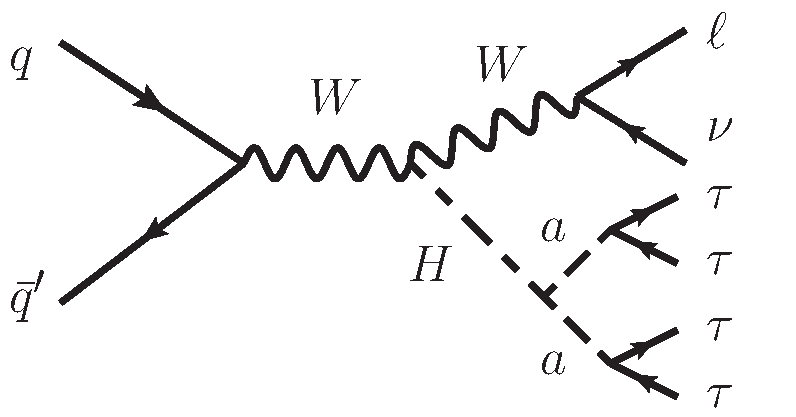
\includegraphics[width=\cmsFigWidth]{figures/FeynWH_ellnu4tau}
    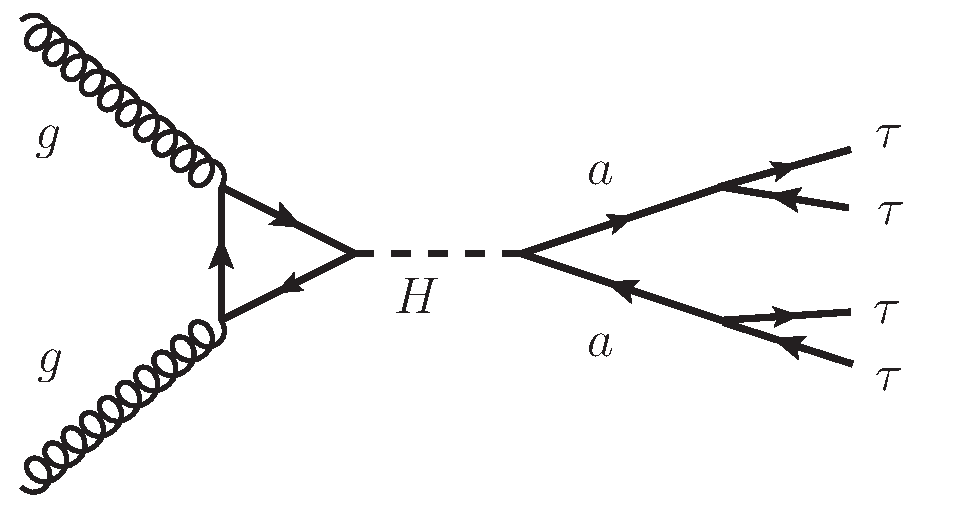
\includegraphics[width=\cmsFigWidth]{figures/FeynggH_aa_4tau}
    \caption{Feynman diagrams of signal processes. (\cmsLeft) $W$ associated production channel. (\cmsRight) Gluon fusion production channel.}
    \label{fig:signatures}
  \end{center}
\end{figure}

\section{Motivations\label{sec:motivations}}

\subsection{Light pseudoscalars\label{sec:lighta}}
% Explain how some models allow light (pseudo)scalars, under what conditions this can occur, and what the expected cross-sections are --> ask Jack.
Following the discovery by the CMS and ATLAS experiments at the LHC~\cite{Aad:2012tfa,Chatrchyan:2012ufa} of a Higgs-like particle $H$, additional measurements of its properties using the full data sets at $\sqrt{s}$ = 7 and 8 TeV reveal that the observed state with a mass near 125.5 GeV is quite consistent with the standard model (SM)~\cite{ATLASnew,CMS:new,Aad:2013wqa}. It is thus clear that models with an extended Higgs sector are significantly constrained by the data.  Consequently, it is interesting to explore the important possibility~\cite{Dermisek:2005ar,Dermisek:2006wr} that decays of the type $H$$\rightarrow$$aa$ (where $a$ is a lighter pseudoscalar) or $H$$\rightarrow$$hh$ (where $h$ is a lighter scalar) are present (for reviews, see~\cite{Chang:2008cw,Curtin:2013fra}). Such decays are certainly possible in the context of various extensions of the SM, including two Higgs doublet models (2HDM), the next-to-minimal supersymmetric standard model (NMSSM), and purely Higgs-sector models containing additional singlet Higgs fields, but notably are not possible in the (CP-conserving) minimal supersymmetric standard model (MSSM) because of the tightly constrained nature of its Higgs sector. 2HDM studies that consider, at least briefly, the possible decays of the observed SM-like Higgs to a pair of lighter Higgs bosons include~\cite{Celis:2013rcs,Grinstein:2013npa,Coleppa:2013dya,Chen:2013rba,Craig:2013hca,Wang:2013sha,Curtin:2013fra,Baglio:2014nea}. Studies in the NMSSM or NMSSM-like context include~\cite{King:2012tr,Cao:2013gba,Christensen:2013dra,Cerdeno:2013cz,Curtin:2013fra} and studies in the general case of adding a singlet field to the SM or the 2HDM can be found in~\cite{Chalons:2012qe,Ahriche:2013vqa,Curtin:2013fra}.

The branching ratio for the $H$ to decay to two lighter Higgs bosons is limited by the apparently SM-like nature of the $H$. An often-studied option is that of $H$ decays to invisible states. However, limits obtained under the assumption of invisibility do not apply to Higgs pair states, which should rather be thought of as simply unseen, $U$, decay modes. The most thorough study for this case is that of~\cite{Belanger:2013xza} which combines CMS and ATLAS data. There it is found at 95\% C.L. that: Br($H$$\rightarrow$$U$) $\le$ 0.21 for a Higgs with completely SM-like couplings; Br($H$$\rightarrow$$U$) $\le$ 0.31 for a SM Higgs but allowing for extra loop contributions to its $\gamma\gamma$ and gg couplings; and Br($H$$\rightarrow$$U$) $\le$ 0.39 if the couplings to up quarks, down quarks and vector bosons are allowed to vary within a general model with only doublets and singlets in the Higgs sector (and no extra loop contributions to the gg and $\gamma\gamma$ couplings). If the up, down and vector boson couplings are allowed to vary completely freely, then all LHC rates can be reproduced if all the couplings-squared are increased by a factor of 1/(1-Br($H$$\rightarrow$$U$)). The only limit in this latter case arises from direct limits on the observed Higgs total width.  At the moment, this is at the level of $\Gamma_{\text{tot}} \le 4\Gamma_{\text{tot}}^{\text{SM}}$~\cite{CMSHwidth}. If the couplings-squared are all increased by 1/(1-Br($H$$\rightarrow$$U$)), the rates for $gg$$\rightarrow$$H$$\rightarrow$$U$ and other production mechanisms are all increased by a factor of Br($H$$\rightarrow$$U$)/(1-Br($H$$\rightarrow$$U$)), making such modes even more accessible. However, even if one adopts the more conservative approach of only considering doublets+singlets models, there is still an excellent prospect for seeing Higgs pair modes if Br($H$$\rightarrow$$U$) $\la$ 0.39.  

Indeed, almost any branching ratio for $H$$\rightarrow$$aa$ or $H$$\rightarrow$$hh$ is possible and imposing Br($H$$\rightarrow$$U$) $\la$ 0.39 significantly constrains 2HDM+singlets theories.  This is because the required $H$$\rightarrow$$aa$ or $H$$\rightarrow$$hh$ couplings are inevitably present and are generically sizeable, and are sufficiently large that to avoid $\Gamma$($H$$\rightarrow$$aa$,$hh$) $\gg$ $\Gamma$($H$$\rightarrow$$b\bar{b}$) requires significant parameter tuning (assuming $m_a$, $m_h$ < $m_H$/2). For example, in the NMSSM (where the pseudoscalar mass eigenstate is defined by $a$ = $\cos\theta_A$ $a_{\text{MSSM}}$ + $\sin\theta_A$ $a_S$, with $a_{\text{MSSM}}$ being the MSSM-like pseudoscalar and $a_S$ the singlet pseudoscalar of the NMSSM). $\abs{\cos\theta_A}$ $\ll$ 1 is generically needed to keep the Haa coupling small by suppressing the doublet content of the $a$.  In the 2HDM, fine-tuned relations among the parameters of the model are required for acceptably small ($\la 0.2$) Br($H$$\rightarrow$$aa$) or Br($H$$\rightarrow$$hh$).

Direct constraints on the $a$ or $h$ play a role in assessing the possibilities. A previous CMS result~\cite{Chatrchyan:2012am} (based on~\cite{Dermisek:2009fd}) places limits on $\sigma$($pp$$\rightarrow$$aa$$\rightarrow$$\mu\mu$) on the order of 2\mdash6 pb in the mass range from 5\mdash14 GeV, excluding the upsilon resonance region.  These limits, despite being based on just 1.3 fb$^{-1}$ of 7 TeV data, can impact models. For example,~\cite{Chatrchyan:2012am} shows that they significantly constrain the $\cos\theta_A$ mixing angle factor defining the NMSSM.  The constraints on $\abs{\cos\theta_A}$ are especially strong at large $\tan\beta$, where $\tan\beta$ is defined as the ratio of the neutral Higgs vacuum expectation values in the MSSM. In the case of the single $a$ = $a_{\text{MSSM}}$ state of the CP-conserving 2HDM, points in the parameter space that are consistent with $m_H \sim$ 125.5 GeV fits at 95\% C.L. and other LHC and pre-LHC constraints violate this limit in the case of Type~II models (but not in the case of Type~I)~\cite{Dumont:2014wha}.  However, in general such constraints do not significantly restrict Br($H$$\rightarrow$$aa$) or Br($H$$\rightarrow$$hh$).  

The techniques appropriate for detecting a Higgs-pair decay mode depend crucially on the mass of the lighter Higgs boson. One important possibility, particularly prominent in the NMSSM, is that the lightest CP-odd state $a$ has mass below or not far above $2m_b$. Small $m_a$ arises naturally in the limit of a so-called $U(1)_R$ symmetry of the model. However, a small mass for the light Higgs states is generically possible in all the models listed earlier. In addition, even if the light Higgs boson has mass above $2m_b$ (but, of course, below $m_H$/2) the $\tau\tau$ mode will still have a branching ratio of order 0.045 and will have smaller backgrounds than a purely 4$b$ final state or the $b\bar{b}\tau\tau$ final state. Thus, a generic exploration of the sensitivity in the $4\tau$ final state is of considerable interest, especially as more and more integrated luminosity is accumulated in future running.

\subsection{Semileptonic di-tau decays\label{sec:semileptonic}}
This search explores the current level of sensitivity to the $4\tau$ final state, and techniques are developed for isolating this final state from backgrounds. In particular, at least one of the tau pairs produced in the decays of the light Higgs bosons is required to decay semileptonically as $\tau_{\mu}\tau_{\text{had}}$. Requiring at least one hadronic tau decay is intended to maximize statistics, due to the higher branching ratio for hadronic tau decays -- 64.76\% compared to 17.41\% and 17.83\% for decays to muons or electrons respectively~\cite{Agashe:2014kda}. However, the choice for the other tau not to decay hadronically was motivated by issues with the reconstruction of boosted tau pairs.

Because of the large mass difference between the $H$ and $a$, the final-state tau pairs are highly collimated, resulting in the overlap of their decay products. This spoils the isolation of the individual taus and renders their reconstruction difficult or impossible by standard means. In order to reconstruct boosted $\tau\tau$ pairs, a modified version of the standard hadron plus strips (HPS)~\cite{CMS:2011msa} tau reconstruction procedure has been developed for this search. This method, described fully in Section~\ref{sec:evtsel-tauID}, involves identifying and removing a leptonic tau decay candidate (muon or electron) from the PF jet used to seed the hadronic tau decay reconstruction. As this method has been successful in recovering hadronic tau ID efficiency, this search has thus focused on the reconstruction of semileptonic boosted tau decays -- in particular, only $\tau_{\mu}\tau_{\text{had}}$ decays, due to the relative ease and cleanness with which low-$p_T$ muons are reconstructed at CMS compared to electrons.

\section{Datasets\label{sec:datasets}}
%%%%%%%%%%%%%%%%%%%

\subsection{Data samples and trigger\label{sec:datasets-data}}
The datasets used in this search are the most recent \texttt{SingleMu} primary datasets collected by CMS in 2012 at $\sqrt{s}$ = 8 TeV.  The high level trigger (HLT) path \texttt{HLT\_IsoMu24\_eta2p1} requires the presence of at least one isolated muon with $p_T >$ 24 GeV found within the CMS muon coverage of $\abs{\eta} <$ 2.1.  More details about the HLT muon reconstruction and isolation requirement can be found in Ref.~\cite{HLTMenus}.  These datasets, listed in Table~\ref{tab:Data}, correspond to an integrated luminosity of 19.7 fb$^{-1}$. The JSON file used in the search for bad data masking can be found at \texttt{/afs/cern.ch/cms/CAF/CMSCOMM/COMM\_DQM/certification/Collisions12/8TeV/\\Reprocessing/Cert\_190456-208686\_8TeV\_22Jan2013ReReco\_Collisions12\_JSON.\\txt}.

\begin{table}
\begin{center}
\singlespacing
\begin{tabular}{ll}
	\hline
	Dataset name & Run range \\
	\hline
	\texttt{/SingleMu/Run2012A-22Jan2013-v1/AOD} & 190456-193621 \\
	\texttt{/SingleMu/Run2012B-22Jan2013-v1/AOD} & 193833-196531 \\
	\texttt{/SingleMu/Run2012C-22Jan2013-v1/AOD} & 198022-203742 \\
	\texttt{/SingleMu/Run2012D-22Jan2013-v1/AOD} & 203777-208686 \\
	\hline
\end{tabular}
\caption{Data samples.}
\label{tab:Data}
\end{center}
\end{table}

\subsection{Monte Carlo samples\label{sec:datasets-MC}}
The Monte Carlo (MC) samples used for the backgrounds outlined in the introduction are listed in Table~\ref{tab:MCBkg}.

\begin{sidewaystable}
\begin{center}
\caption{Monte Carlo background samples. Cross sections from \cite{PREP} and \cite{8TeVTwiki}.\label{tab:MCBkg}}
\singlespacing
\resizebox{\textwidth}{!}{\begin{tabular}{| l | l |}
        \hline
	Dataset name & \begin{tabular}[c]{@{}l@{}}Cross \\section (pb)\end{tabular} \\
	\hline
	\hline
	\texttt{/W1JetsToLNu$\_$TuneZ2Star$\_$8TeV-madgraph/Summer12$\_$DR53X-PU$\_$S10$\_$START53$\_$V7A-v1/AODSIM} & 6601.5 \\
	\texttt{/W2JetsToLNu$\_$TuneZ2Star$\_$8TeV-madgraph/Summer12$\_$DR53X-PU$\_$S10$\_$START53$\_$V7A-v1/AODSIM} & 2110.3 \\
	\texttt{/W3JetsToLNu$\_$TuneZ2Star$\_$8TeV-madgraph/Summer12$\_$DR53X-PU$\_$S10$\_$START53$\_$V7A-v1/AODSIM} & 633.6 \\
	\texttt{/W4JetsToLNu$\_$TuneZ2Star$\_$8TeV-madgraph/Summer12$\_$DR53X-PU$\_$S10$\_$START53$\_$V7A-v1/AODSIM} & 214 \\
	\texttt{/DYJetsToLL$\_$M-10To50$\_$TuneZ2Star$\_$8TeV-madgraph/Summer12$\_$DR53X-PU$\_$S10$\_$START53$\_$V7A-v1/AODSIM} & 14702 \\
	\texttt{/DYJetsToLL$\_$M-50$\_$TuneZ2Star$\_$8TeV-madgraph-tarball/Summer12$\_$DR53X-PU$\_$S10$\_$START53$\_$V7A-v1/AODSIM} & 3503.71 \\
	\texttt{/TTJets$\_$MassiveBinDECAY$\_$TuneZ2star$\_$8TeV-madgraph-tauola/Summer12$\_$DR53X-PU$\_$S10$\_$START53$\_$V7A-v2/AODSIM} & 245.8 \\
	\texttt{/T$\_$s-channel$\_$TuneZ2star$\_$8TeV-powheg-tauola/Summer12$\_$DR53X-PU$\_$S10$\_$START53$\_$V7A-v1/AODSIM} & 3.79 \\
	\texttt{/T$\_$t-channel$\_$TuneZ2star$\_$8TeV-powheg-tauola/Summer12$\_$DR53X-PU$\_$S10$\_$START53$\_$V7A-v1/AODSIM} & 56.4 \\
	\texttt{/Tbar$\_$s-channel$\_$TuneZ2star$\_$8TeV-powheg-tauola/Summer12$\_$DR53X-PU$\_$S10$\_$START53$\_$V7A-v1/AODSIM} & 1.76 \\
	\texttt{/Tbar$\_$t-channel$\_$TuneZ2star$\_$8TeV-powheg-tauola/Summer12$\_$DR53X-PU$\_$S10$\_$START53$\_$V7A-v1/AODSIM} & 30.7 \\
	\texttt{/WW$\_$TuneZ2star$\_$8TeV$\_$pythia6$\_$tauola/Summer12$\_$DR53X-PU$\_$S10$\_$START53$\_$V7A-v1/AODSIM} & 54.838 \\
	\texttt{/WZ$\_$TuneZ2star$\_$8TeV$\_$pythia6$\_$tauola/Summer12$\_$DR53X-PU$\_$S10$\_$START53$\_$V7A-v1/AODSIM} & 33.21 \\
	\texttt{/ZZ$\_$TuneZ2star$\_$8TeV$\_$pythia6$\_$tauola/Summer12$\_$DR53X-PU$\_$S10$\_$START53$\_$V7A-v1/AODSIM} & 17.654 \\
	\hline
\end{tabular}}
\end{center}
\end{sidewaystable}

The Monte Carlo signal samples for associated WH production and gluon fusion production were generated with PYTHIA~\cite{1126-6708-2006-05-026} and reconstructed with CMSSW version 5.3 using the \texttt{S10} pileup scenario. The $W$ in the associated $W$ production sample is constrained to decay only leptonically. Since PYTHIA does not model NMSSM processes, the production and decay of the NMSSM scalar and pseudoscalar Higgs particles were approximated using PYTHIA's two Higgs doublet model instead. A separate sample of signal events was generated using MADGRAPH~\cite{springerlink:10.1007/JHEP06(2011)128}, which does contain methods for modeling NMSSM processes directly, and the kinematics of the PYTHIA and MADGRAPH event samples were shown to be compatible and equivalent. The benchmark for this search takes the masses of the NMSSM $a$, $h_1$, $h_2$, and $h_3$ to be 9, 125, 500, and 500 GeV respectively; a mass scan is performed over $m_{a}$ from 5 to 15 GeV in increments of 2 GeV.  The assumed cross sections for each signal sample are given in Table~\ref{tab:MC-sig}.  These are the cross sections for SM 125 GeV Higgs production at 8 TeV~\cite{LHCHXSWG} multiplied by BR($H\rightarrow$$aa\rightarrow4\tau$) = 100\%, which is why the cross sections are constant with pseudoscalar mass.  The $W\rightarrow$ leptons branching ratio is included in the quoted cross sections for the WH signals.

\begin{table*}[htbh]
\begin{center}
\caption{Assumed signal MC cross sections.\label{tab:MC-sig}}
\singlespacing
\begin{tabular}{|c|c|c|}
\hline
\multicolumn{2}{|c|}{} & Cross section (pb) \\
\hline
\multirow{5}{*}{WH} & $m_{a}$ = 5 GeV & 0.2296\\
& $m_{a}$ = 7 GeV & 0.2296\\
& $m_{a}$ = 9 GeV & 0.2296\\
& $m_{a}$ = 11 GeV & 0.2296\\
& $m_{a}$ = 13 GeV & 0.2296\\
& $m_{a}$ = 15 GeV & 0.2296\\
\hline
\multirow{5}{*}{ggH} & $m_{a}$ = 5 GeV & 19.27\\
& $m_{a}$ = 7 GeV & 19.27\\
& $m_{a}$ = 9 GeV & 19.27\\
& $m_{a}$ = 11 GeV & 19.27\\
& $m_{a}$ = 13 GeV & 19.27\\
& $m_{a}$ = 15 GeV & 19.27\\
\hline
\multirow{5}{*}{ZH} & $m_{a}$ = 5 GeV & 0.4153\\
& $m_{a}$ = 7 GeV & 0.4153\\
& $m_{a}$ = 9 GeV & 0.4153\\
& $m_{a}$ = 11 GeV & 0.4153\\
& $m_{a}$ = 13 GeV & 0.4153\\
& $m_{a}$ = 15 GeV & 0.4153\\
\hline
\multirow{5}{*}{VBF} & $m_{a}$ = 5 GeV & 1.578\\
& $m_{a}$ = 7 GeV & 1.578\\
& $m_{a}$ = 9 GeV & 1.578\\
& $m_{a}$ = 11 GeV & 1.578\\
& $m_{a}$ = 13 GeV & 1.578\\
& $m_{a}$ = 15 GeV & 1.578\\
\hline
\end{tabular}
\end{center}
\end{table*}

\subsection{Higgs transverse momentum reweighting for ggH\label{sec:datasets-higgsptreweight}}

In gluon fusion Higgs production, the Higgs $p_T$ spectrum can be significantly affected by next-to-leading logarithmic (NLL) and next-to-next-to-leading logarithmic (NNLL) corrections, especially in the low-$p_T$ range~\cite{Bozzi:2003jy}. Thus, a set of weights binned in $p_T$, calculated with the Higgs $p_T$-reweighting HqT software \cite{HQTDocumentation}, was applied to the Higgs $p_T$ spectrum of signal MC events in the ggH production channel. The effect of this reweighting was observed to be quite small, as it produced a change of less than 2\% in signal-to-background ratio for each signal and a change of less than 2.5\% in the number of each type of signal event passing the final selection.

\subsection{ZH and VBF production channels\label{sec:datasets-zhvbf}}

A study was done to assess the contribution of ZH and VBF production channels to the expected signal significance. ZH and VBF signal samples were generated for pseudoscalar mass point $m_{a}$ = 9 GeV and the numbers of events passing the full selection sequence were normalized to 19.7 fb$^{-1}$ using the official SM production cross sections for ZH and VBF. Then, expected limits for the WH and ggH signal channels were calculated after the total expected yield of ZH and VBF events was distributed among the WH and ggH expected yields proportionally to their sizes, and these expected limits were compared to the nominal expected limits for WH and ggH without the added events. The combined presence of ZH and VBF signals changed the WH and ggH expected limits by at most 10\%, and the change was always well within the $1\sigma$ error band of the nominal expected limits. Yet, in the low-$M_{T}$ bin, the contribution of VBF was larger than that of WH, so ultimately it was concluded that the contributions of VBF and ZH should be considered too.

However, due to a shortage of time, ZH and VBF MC samples could not be generated for the other pseudoscalar mass points. Instead, the contribution of VBF for each pseudoscalar mass point was estimated by taking the number of surviving ggH events in the counting experiment bin after the full selection and normalizing this number to the expected SM VBF production cross-section, since the selection efficiency is expected to be the same for ggH and VBF topologies; effects due to the different $H$ $p_T$ spectra for the two topologies were found not to be significant. Also, since ZH and WH are expected to have similar selection efficiencies (with the ZH trigger efficiency being 1.1 times higher than for WH due to the decay of \Z to two high-$p_T$ muons rather than one), the contribution of ZH at each pseudoscalar mass point was estimated similarly by rescaling the WH contribution to the expected SM ZH production cross-section.

In the high-$M_{T}$ bin, since the contributions of ZH and VBF are considerably smaller than those of WH and ggH, these estimated yields are treated as nuisance parameters, while the WH and ggH channels are used for setting limits. In the low-$M_{T}$ bin, the ggH channel is dominant, and the contribution of the VBF channel is larger than that of WH and ZH, so WH and ZH are treated as nuisance parameters while ggH and VBF are used for setting limits. %motivations
\chapter{Event selection\label{sec:evtsel}}

For the events passing the high-level trigger \texttt{HLT\_IsoMu24\_eta2p1}, a series of selection cuts has been developed to identify the most important physics objects in the signal -- the high-$p_T$ trigger muon, the tau decay muon $\tau_{\mu}$ from one leg of the $a$($h$) decay, and the tau $\tau_{\text{had}}$ from the other leg of the $a$($h$) decay -- and optimize the signal sensitivity. This set of cuts will be referred to as the preselection, and plays a role in the estimation of the background. The physics objects to which the selections are applied are reconstructed via the CMS particle flow (PF) algorithm.
%PF described fully in \cite{CMS:2010eua}

A brief list of the preselection cuts is as follows:

\begin{itemize}
	\item Trigger $\mu$ $p_T$ selection
	\item Trigger $\mu$ ID
	\item Trigger $\mu$ PF relative isolation selection
	\item $\tau_{\mu}$ $p_T$ selection
	\item $\tau_{\mu}$ ID
	\item $\tau_{\text{had}}$ $p_T$ selection
	\item $\tau_{\text{had}}$ HPS decay mode finding discriminator
	\item $\tau_{\text{had}}$ HPS isolation discriminator
	\item Charge requirement: $q(\text{Trigger} \mu) \cdot q(\tau_{\mu}) >$ 0
	\item Charge requirement: $q(\tau_{\text{had}}) \cdot q(\tau_{\mu}) <$ 0
        \item b-jet veto
        \item Neighbouring lepton veto around trigger muon
	\item Requirement of consistency with the primary vertex
\end{itemize}

Finally, events are classified into one of two bins: low transverse mass $M_{\text{T}} \le$ 50 GeV or high transverse mass $M_{\text{T}} >$ 50 GeV, where $M_{\text{T}} = \sqrt{2p_{T}^{\text{Trig}\mu}\ETslash(1 - \cos{\Delta\phi(\text{Trig}\mu, \ETslash)})}$.  The low-$M_{\text{T}}$ bin is sensitive to gluon fusion and VBF signal production, where there is no real $W$, while the high-$M_{\text{T}}$ bin is optimized for WH production.

\section{Trigger muon ID\label{sec:evtsel-triggermu}}

Events are required to have at least one reco muon that satisfies the following criteria:
\begin{itemize}
	\item $p_T >$ 25 GeV (this is at the turn-on point for the HLT used in this search, as shown in \cite{CMS:muonhlttwiki})
	\item $\abs{\eta} <$ 2.1
	\item Tight muon ID:
	\begin{itemize}
		\item The reco muon is reconstructed as a global muon and as a PF muon
		\item The global muon track fit has $\chi^{2}/\text{ndof} <$ 10 and at least one muon chamber hit 
		\item The reco muon has segments in at least 2 muon stations
		\item The reco muon's tracker track has $d_{\text{xy}} <$ 2 mm and $d_{\text{z}} <$ 5 mm
		\item Number of pixel hits $>$ 0
		\item More than 5 tracker layers with hits
	\end{itemize}
	\item Relative isolation $I_{\text{rel}} <$ 0.12, where the $I_{\text{rel}}$ of a muon is defined as the pileup-corrected sum of the transverse energy of the photons and charged and neutral hadrons in a cone of radius $\Delta$R = $\sqrt{\Delta\eta^{2} + \Delta\phi^{2}} =$ 0.4 about the muon divided by the $p_T$ of the muon. This is the tight isolation working point recommended by the CMS Muon POG \cite{CMS:muonidtwiki}.
        \item Isolation from nearby leptons located within a cone of $\Delta$R $=$ 0.4 around the trigger muon, where nearby lepton ID criteria are as follows:
          \begin{itemize}
          \item \textbf{Electrons:} \texttt{reco::GsfElectron} passing PF reconstruction with $p_T >$ 7 GeV and $\abs{\eta} <$ 2.5 (same as~\cite{Chatrchyan:2013mxa})
          \item \textbf{Muons:} PF muon with $p_T >$ 5 GeV and $\abs{\eta} <$ 2.4 passing the soft muon ID described in Section~\ref{sec:evtsel-softmu} and~\cite{CMS:2010uta}
          \item \textbf{Taus:} HPS PF tau with $p_T >$ 10 GeV, $\abs{\eta} <$ 2.3, and passing \texttt{DecayModeFinding} and \texttt{MediumCombinedIsolationDBSumPtCorr} discriminators reconstructed from an AK5 PF jet that has been cleaned of the trigger muon with the same jet-cleaning algorithm described in Section~\ref{sec:evtsel-tauID} (the $p_T$ cut at 10 GeV rather than 20 GeV was chosen to make the veto more stringent)
          \end{itemize}
\end{itemize}

The reco muon passing the above criteria (or, if more than one reco muon passed, the one with the highest $p_T$) is then matched to the object that fired the \texttt{HLT\_IsoMu24\_eta2p1} trigger. This is done by requiring $\Delta$R $<$ 0.1 between the reco muon and the trigger object.

%leptonveto subsection
\subsection{Neighbouring lepton veto for trigger muon\label{sec:evtsel-leptonveto}}

The nearby lepton isolation requirement is motivated by the desire to have a well-understood trigger and PF relative isolation efficiency for the ggH and VBF production modes to which this search is sensitive.  Unlike in the WH and ZH production channels, in which the particle firing the isolated muon trigger is an isolated muon from $W$ or $Z$ decay, the particle firing the isolated muon trigger in the ggH and VBF production channels is a muon coming from a tau decay.  The difference is illustrated in Figure~\ref{fig:WHZH-vs-ggHVBF-trigger}.

\begin{figure}[hbtp]
  \begin{center}
    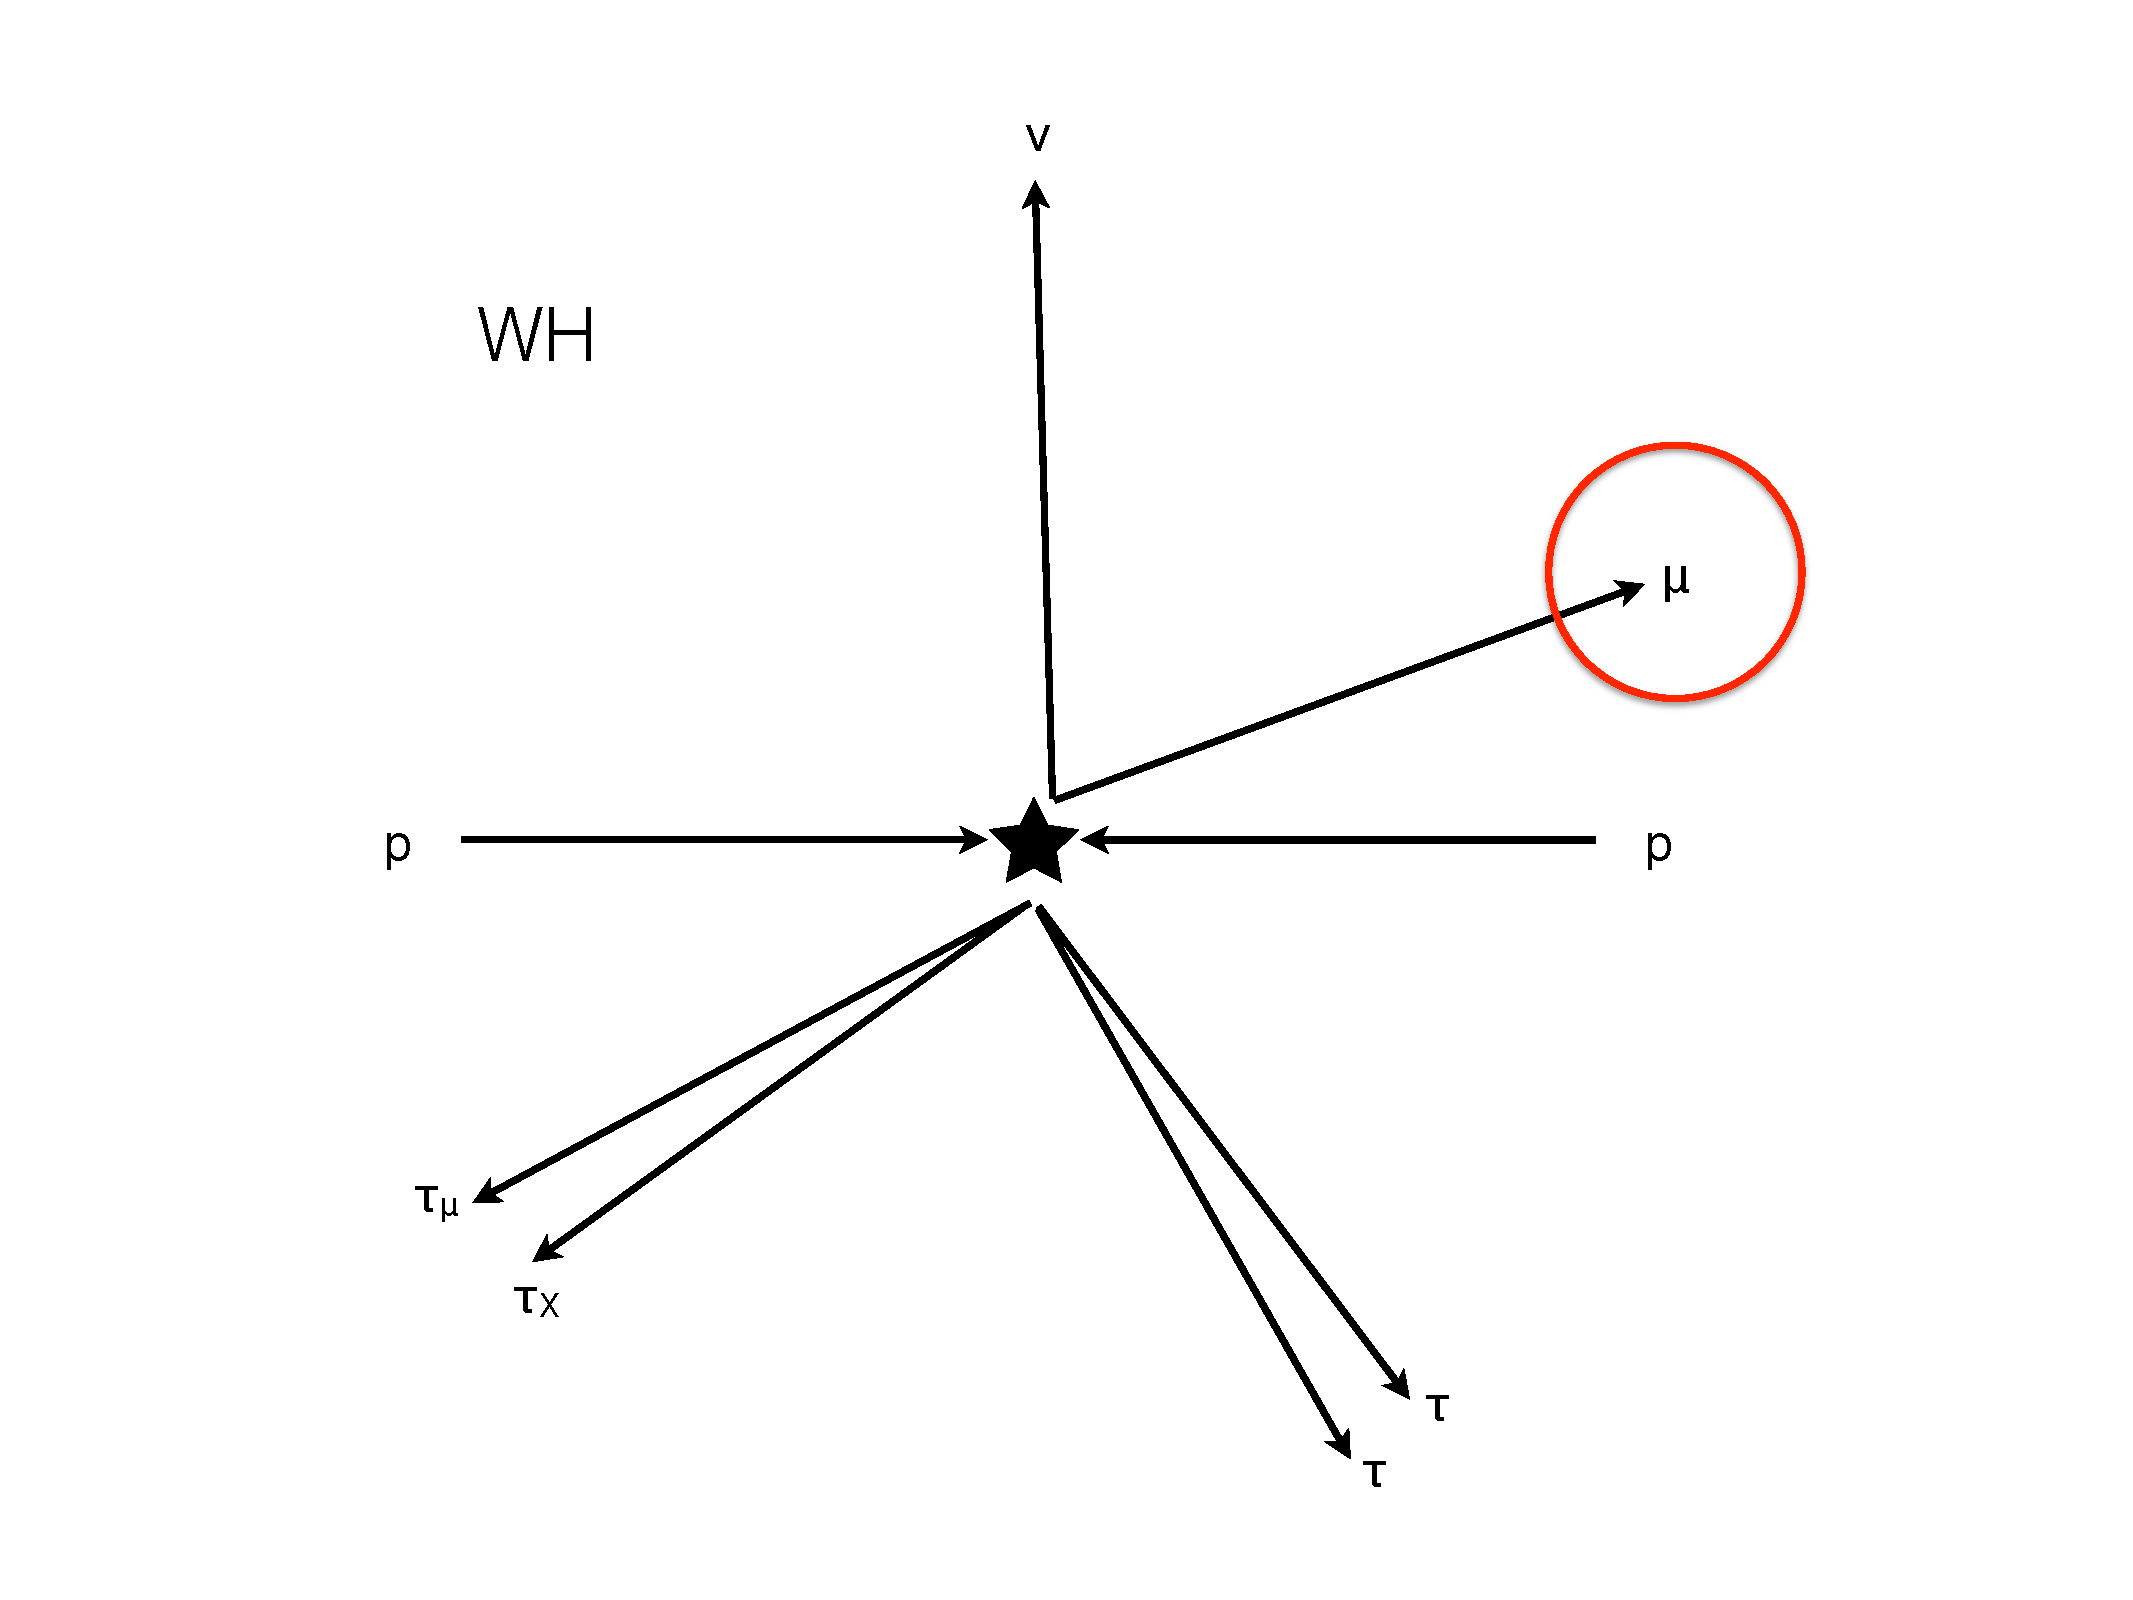
\includegraphics[width=\cmsFigWidth]{figures/WH_trigger}
    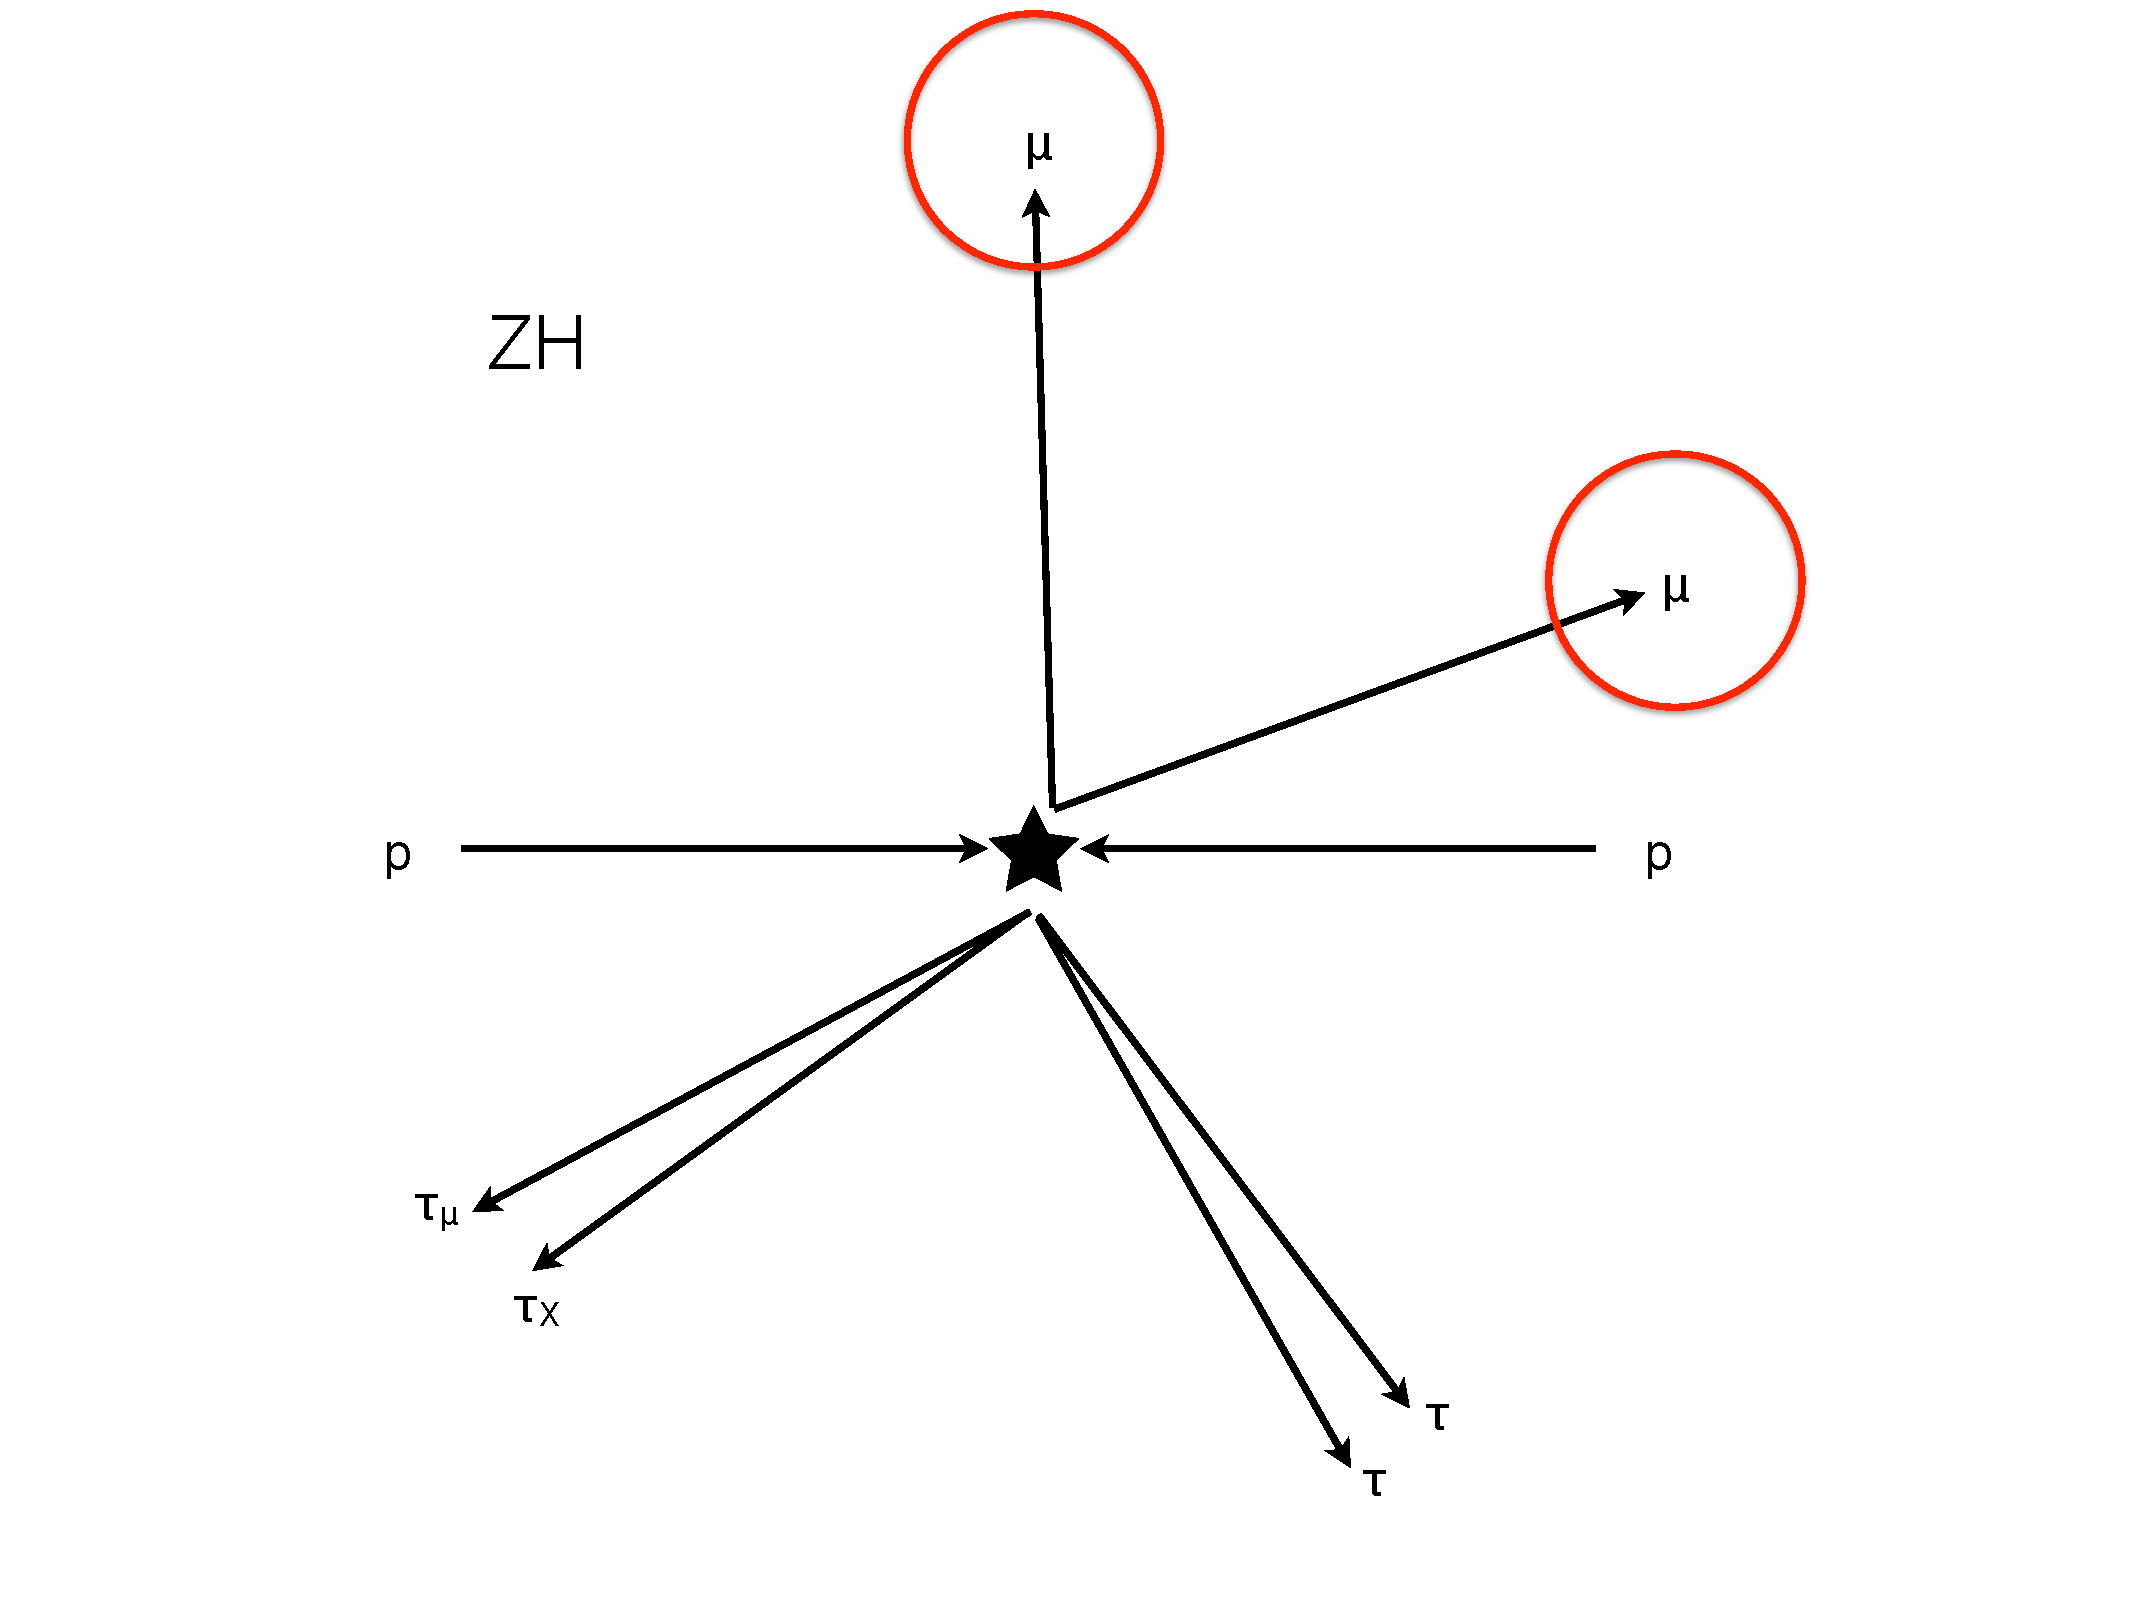
\includegraphics[width=\cmsFigWidth]{figures/ZH_trigger}
    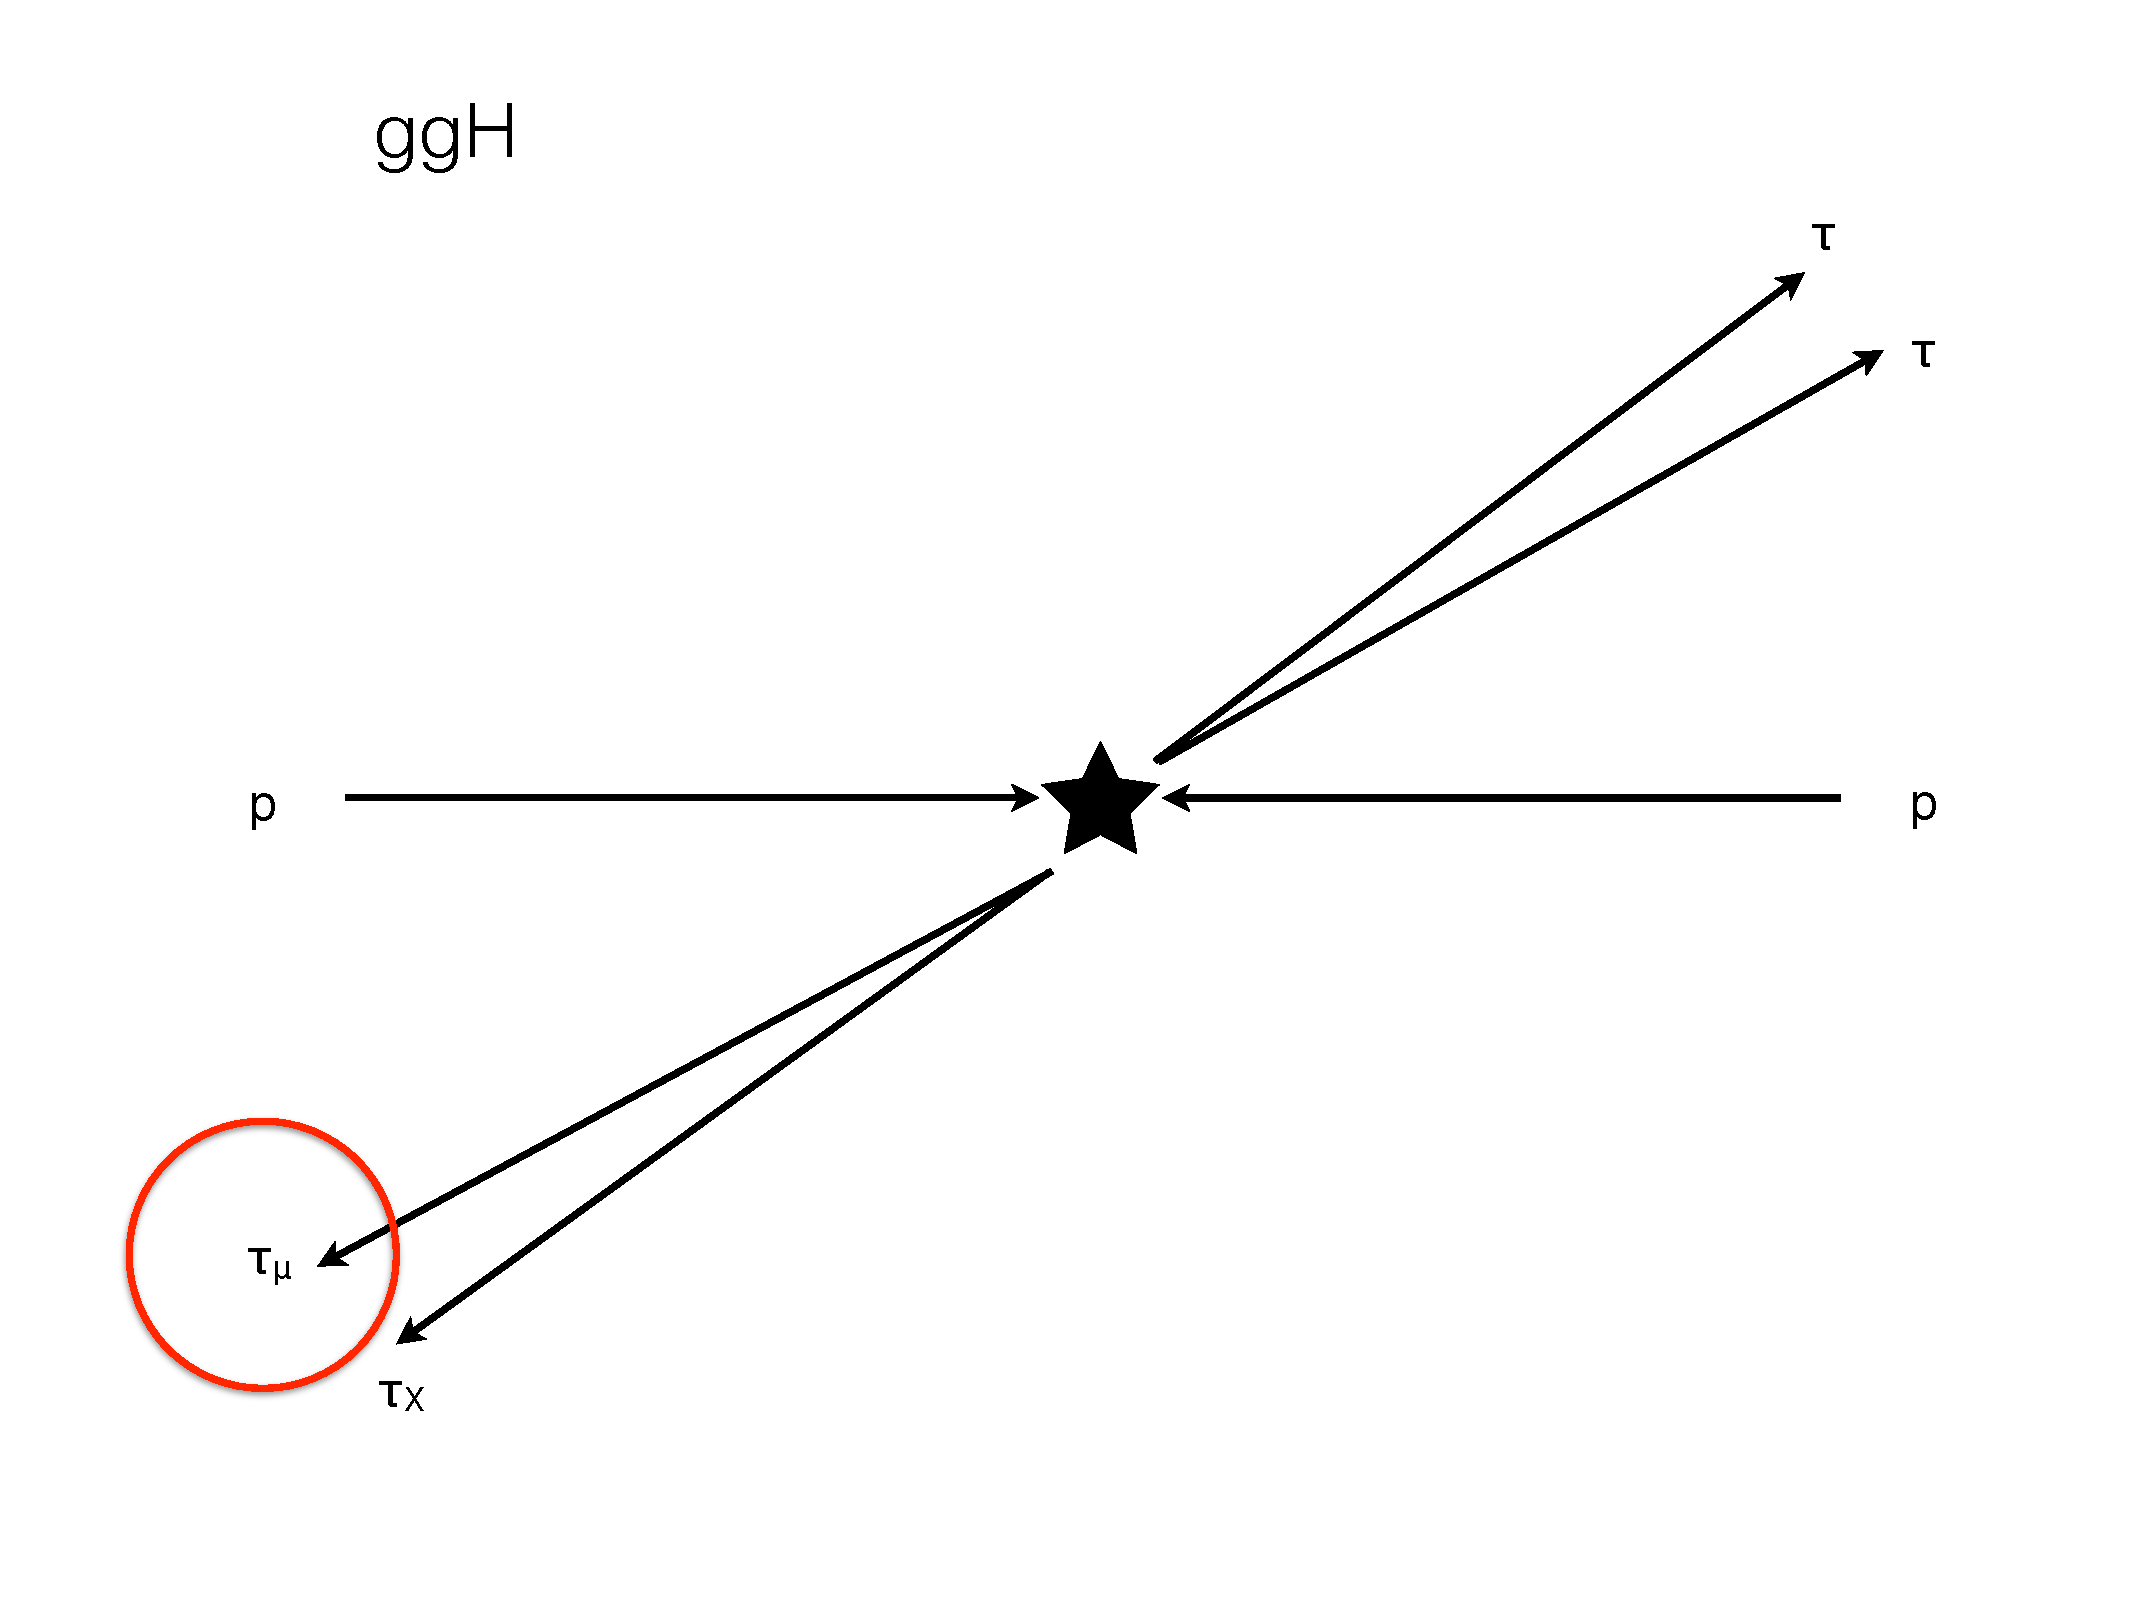
\includegraphics[width=\cmsFigWidth]{figures/ggH_trigger}
    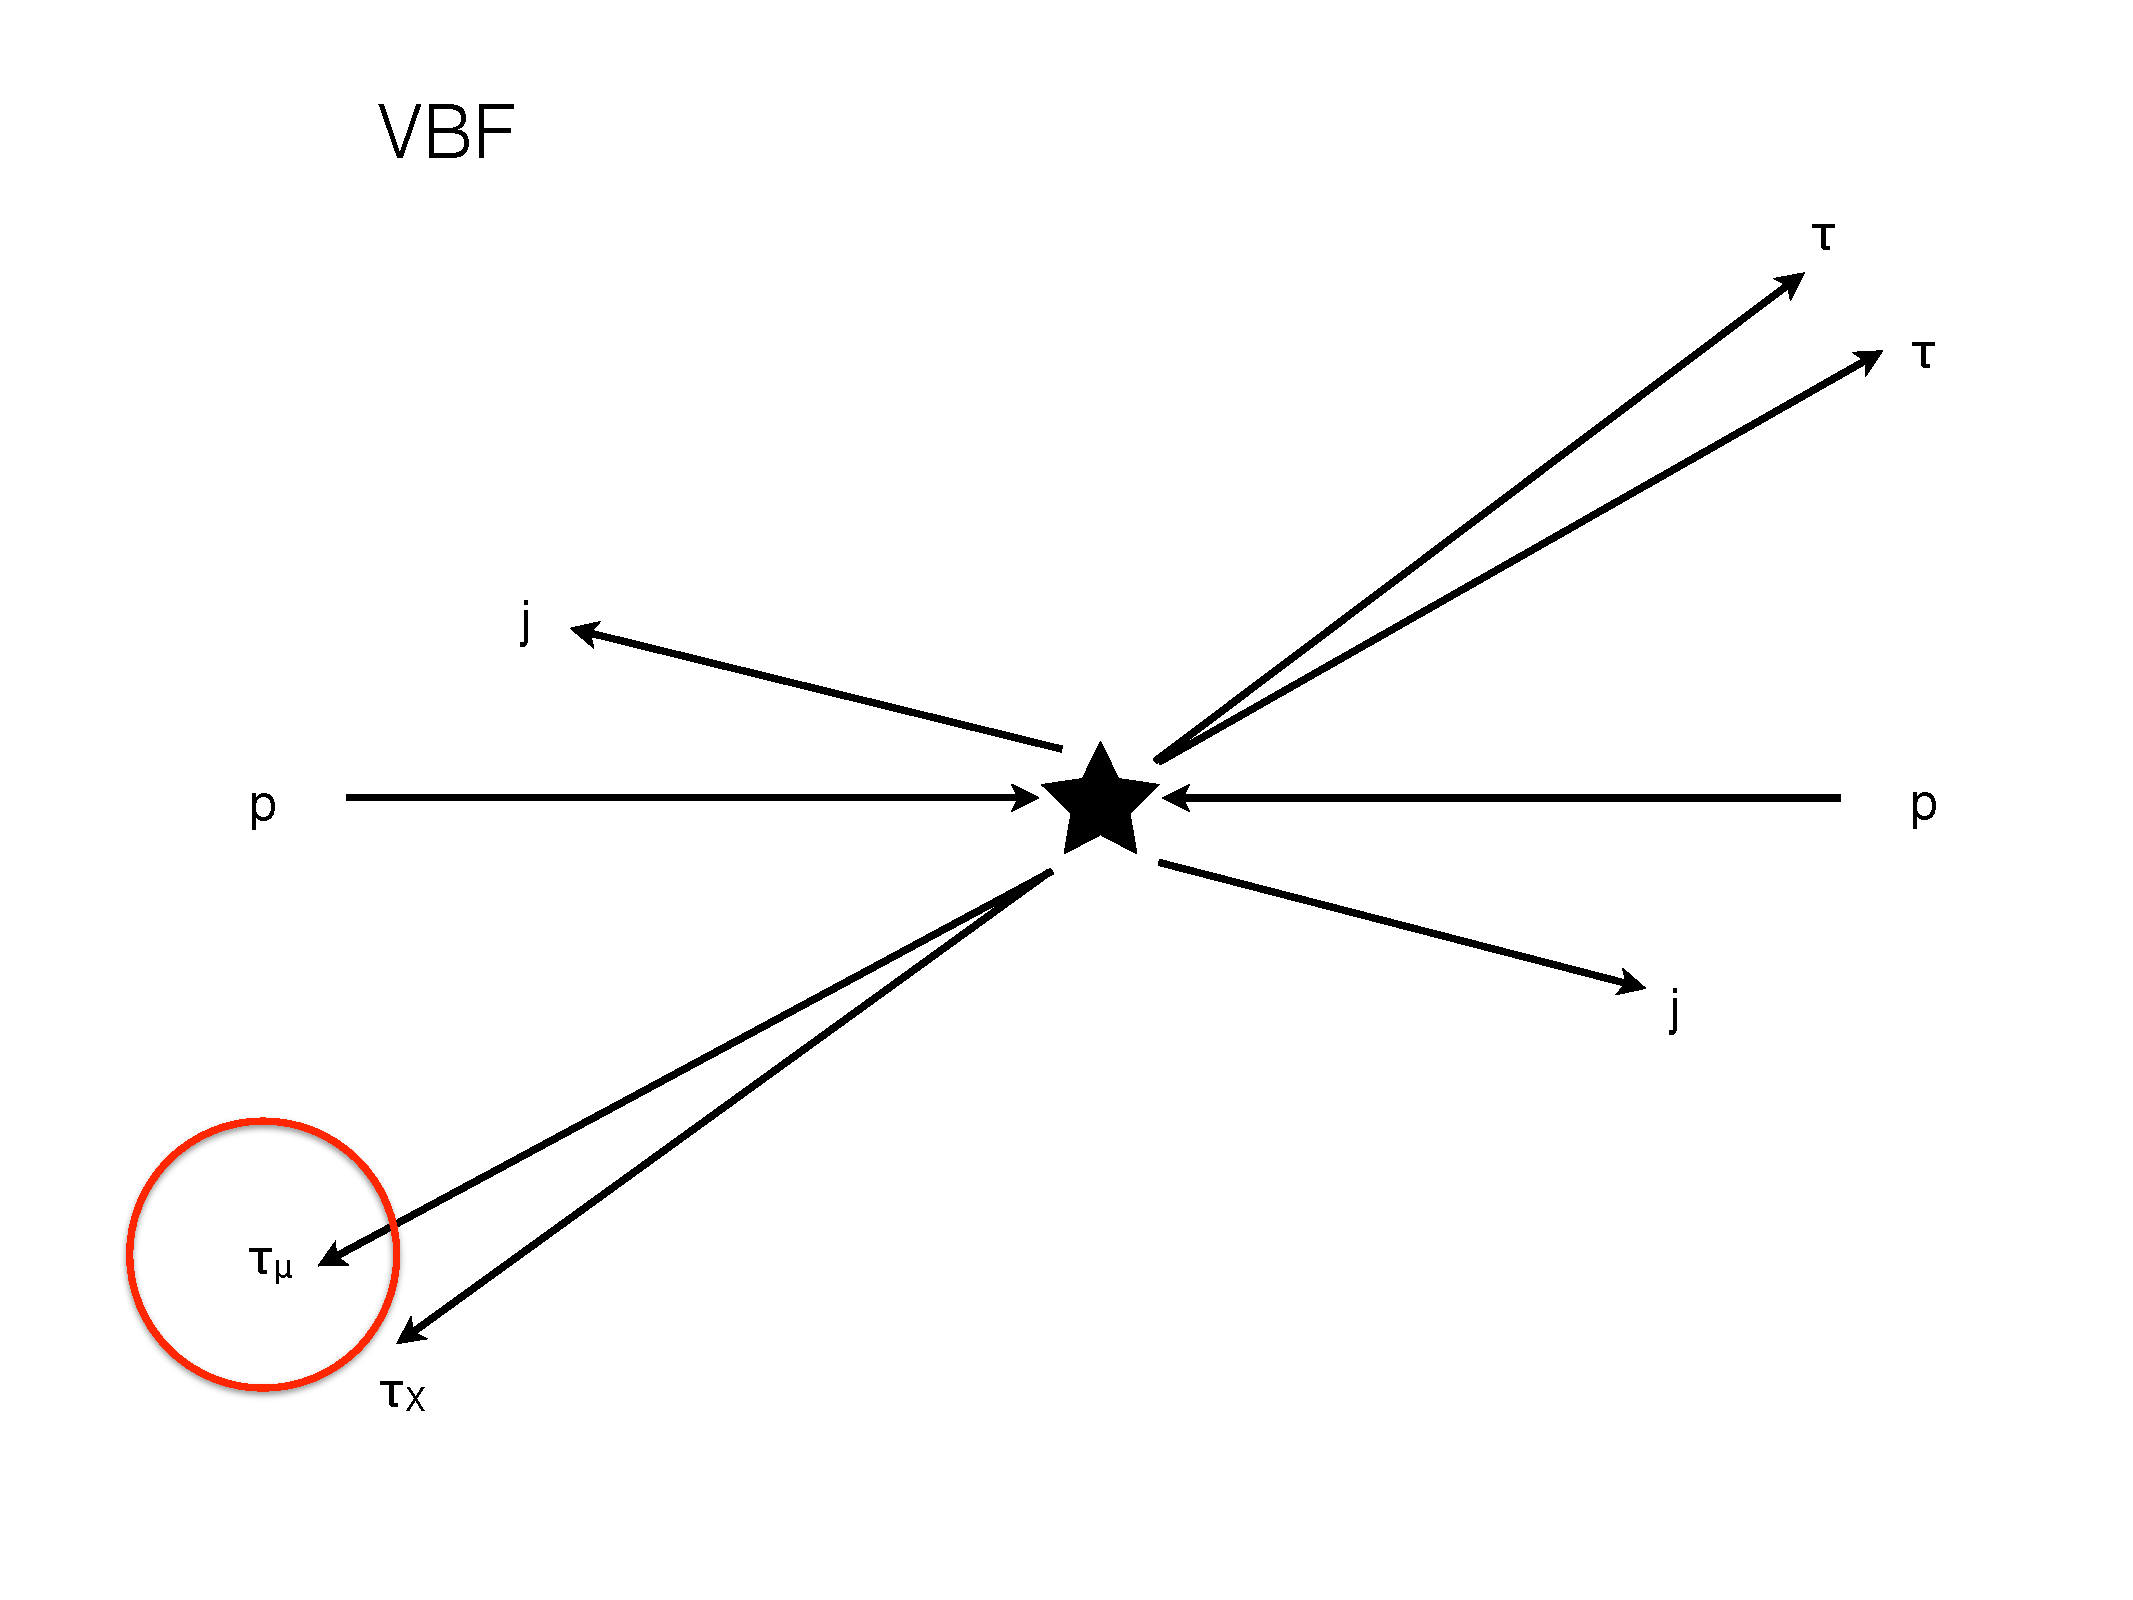
\includegraphics[width=\cmsFigWidth]{figures/VBF_trigger}
    \caption{Diagrams of the four Higgs production modes considered in this search, with the triggering particle circled in red.  (Top \cmsLeft) WH.  (Top \cmsRight) ZH.  (Bottom \cmsLeft) ggH.  (Bottom \cmsRight) VBF.}
    \label{fig:WHZH-vs-ggHVBF-trigger}
  \end{center}
\end{figure}

Due to the boost and low $p_T$ of the pseudoscalar tau decay pairs in ggH and VBF events, most are rejected by \texttt{HLT\_IsoMu24\_eta2p1}.  Those that are accepted fall into two categories:

\begin{enumerate}
\item $a\rightarrow\tau\tau$, one tau decays to a 24 GeV muon and the other tau decays to particles with $p_T$ low enough to pass the HLT muon isolation cut
\item $a\rightarrow\tau\tau$, one tau decays to a 24 GeV muon and the other tau decays far enough away to not be counted in the HLT muon isolation sum
\end{enumerate}

To avoid likely systematic effects in the MC description of ggH and VBF trigger and PF relative isolation efficiency due to the presence of low $p_T$ particles around the trigger muon, events in category 1 are rejected by the nearby lepton isolation requirement.  With this requirement, tau decay muons from the accepted category 2 events appear very similar to muons from $Z$'s or $W$'s, for which \texttt{HLT\_IsoMu24\_eta2p1} and PF relative isolation $<$ 0.12 efficiency measurements and standard scale factors for data-simulation differences are well understood.  The following sections demonstrate that once the nearby lepton isolation requirement is imposed, the efficiency of \texttt{HLT\_IsoMu24\_eta2p1} and PF relative isolation $<$ 0.12 for ggH and VBF tau decay muons in MC is very similar to that of $W$ decay muons in MC.

%HLT efficiency subsection

\subsection{Study of the HLT efficiency for signal events produced via gluon fusion\label{sec:lep-id-eff-ggH-HLT}}
The efficiency for ggH $a\rightarrow\tau\rightarrow\mu$ decay muons to fire \texttt{HLT\_IsoMu24\_eta2p1} is calculated for two reconstructed muon selections.  The first selection is  criteria described in Sec.~\ref{sec:evtsel-triggermu}, except that the nearby lepton isolation requirement is removed.  The second selection is identical to the criteria described in Sec.~\ref{sec:evtsel-triggermu}.  Trigger efficiency is compared for the two selections.  Since the signature of pseudoscalar decays in the detector is similar between the ggH and VBF production modes, the results obtained for ggH simulation can be applied to VBF simulation as well.

The trigger efficiencies of the two selections are given by 

\begin{equation}
\epsilon_{\text{HLT}}^{\text{no }l\text{ iso}} = \frac{\text{No. gen-matched reco'd muons passing no-lepton-isolation ID and HLT}}{\text{No. gen-matched reco'd muons passing trigger muon ID}} \\
\label{eq:muonHLTeff-noliso}
\end{equation}

\begin{equation}
\epsilon_{\text{HLT}} = \frac{\text{No. gen-matched reco'd muons passing trigger muon ID and HLT}}{\text{No. gen-matched reco'd muons passing trigger muon ID}} \\
\label{eq:muonHLTeff}
\end{equation}

where

\begin{itemize}
\item the gen-matching criteria is $\Delta$$p_T$(reco muon, gen $a\rightarrow\tau\rightarrow\mu$ muon) $<$ 0.1 GeV and the gen muon is from the decay of a tau that is itself from the decay of a pseudoscalar;
\item the trigger muon ID for $\epsilon_{\text{HLT}}^{\text{no }l\text{ iso}}$ is as described in Sec.~\ref{sec:evtsel-triggermu} but with the nearby lepton isolation requirement removed;
\item the trigger muon ID for $\epsilon_{\text{HLT}}$ is as described in Sec.~\ref{sec:evtsel-triggermu}; and
\item ``HLT'' refers to firing \texttt{HLT\_IsoMu24\_eta2p1}.
\end{itemize}

Figure~\ref{fig:HLTEffVsDR} shows $\epsilon_{\text{HLT}}^{\text{no }l\text{ iso}}$ as a function of $\Delta$R(gen $a\rightarrow\tau\rightarrow\mu$ muon, gen $\tau_{\text{2}}$), where the gen $a\rightarrow\tau\rightarrow\mu$ muon is matched to the reco'd muon as described in Eq.~\ref{eq:muonHLTeff-noliso} above and the gen $\tau_{\text{2}}$ is the other tau from the $a\rightarrow\tau\tau$ decay.  The efficiency is calculated separately for each decay mode of the gen $\tau_{\text{2}}$ (electronic, muonic, or hadronic).  $\epsilon_{\text{HLT}}^{\text{no }l\text{ iso}}$ is $\sim$90\% for $\Delta$R $>$ 0.4, when the two taus from pseudoscalar decay are separated enough that the tau decay muon appears isolated. This is similar to the efficiency of \texttt{HLT\_IsoMu24\_eta2p1} for $W$ decay muons~\cite{1748-0221-7-10-P10002}.  When the two taus are closer than $\Delta$R $\sim$ 0.4, the efficiency decreases because the non-triggering tau spoils the isolation of the tau decay muon that fires the trigger.  The effect is worst in the $\tau_{\mu}\tau_{e}$ and $\tau_{\mu}\tau_{\mu}$ modes because electrons and muons contribute to isolation at the trigger level, but are not counted in the offline PF relative isolation.

\begin{figure}[hbtp]
  \begin{center}
    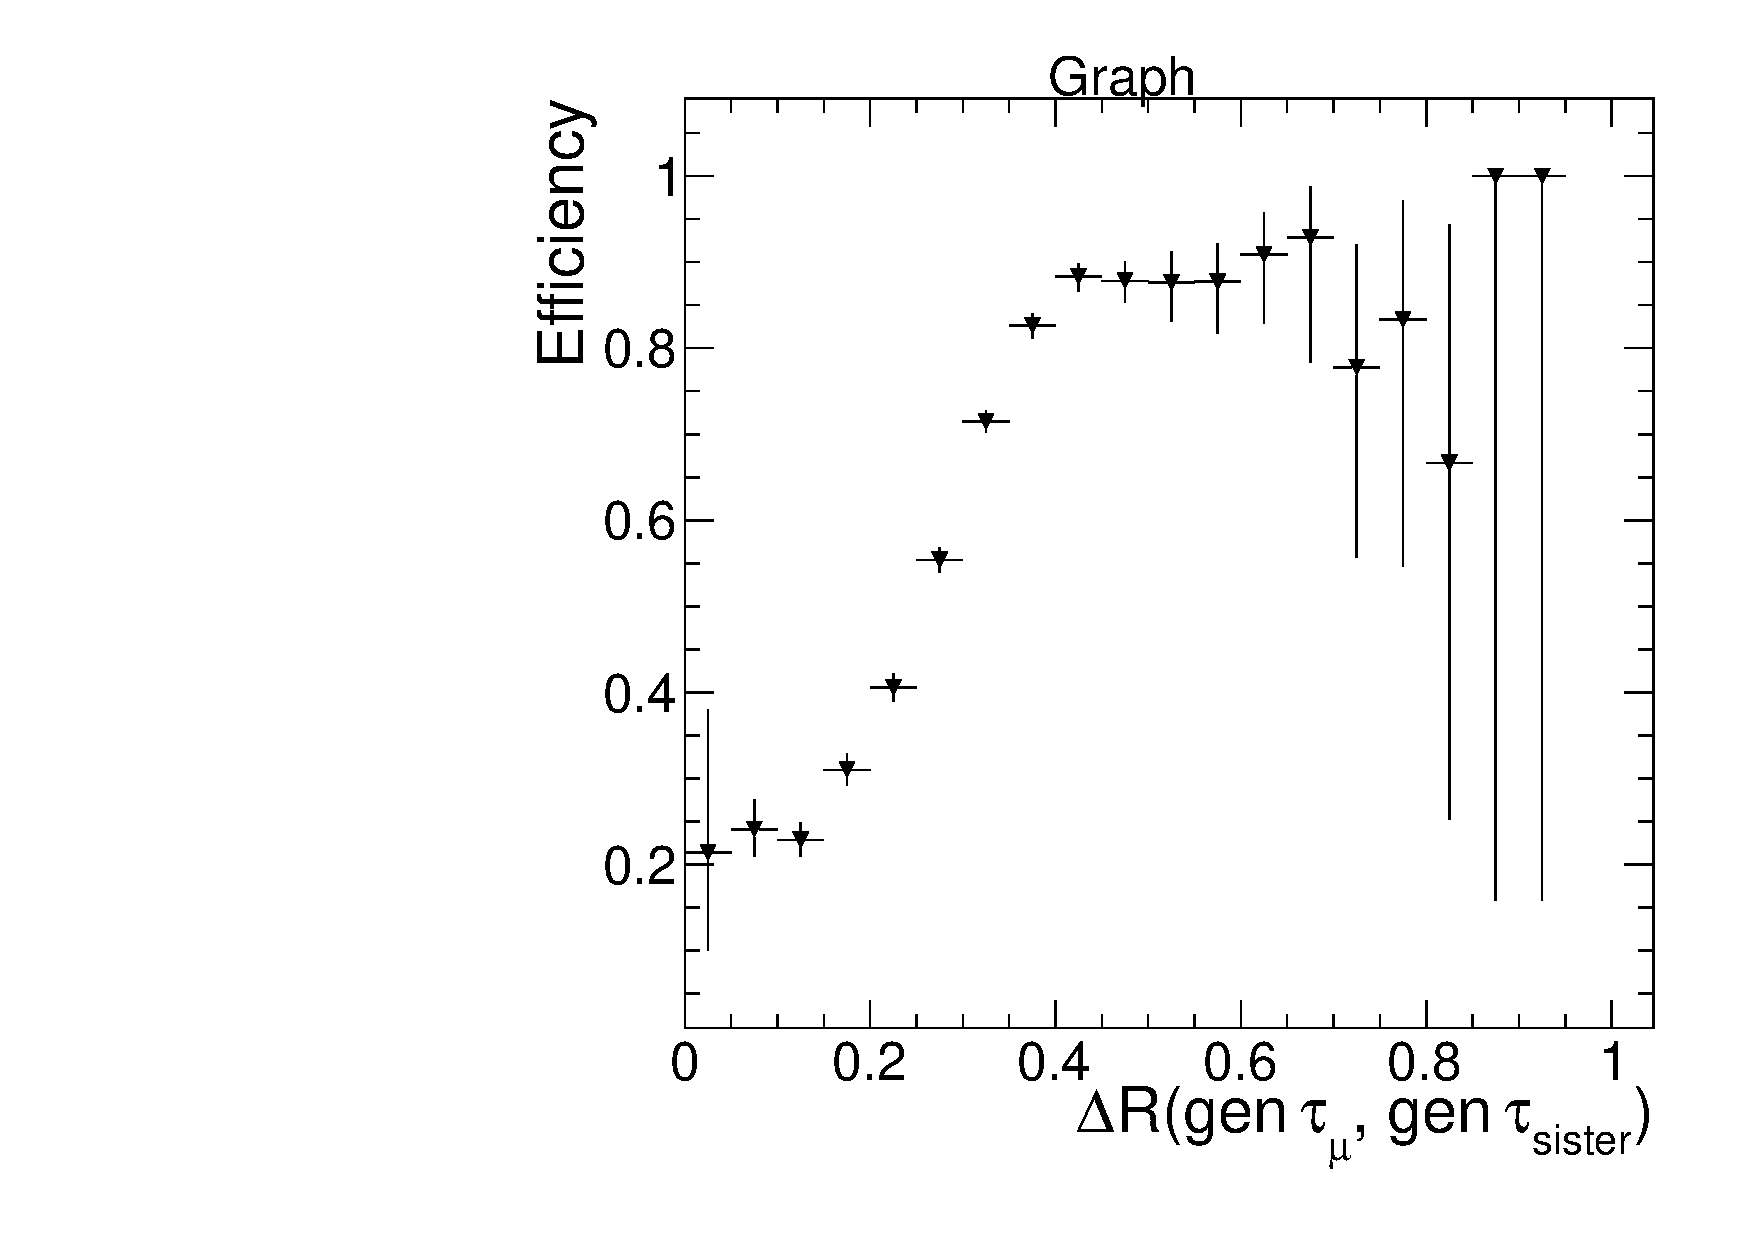
\includegraphics[width=0.8\cmsFigWidth]{figures/dREfficiency_WmuIDIso_muEOnly}
    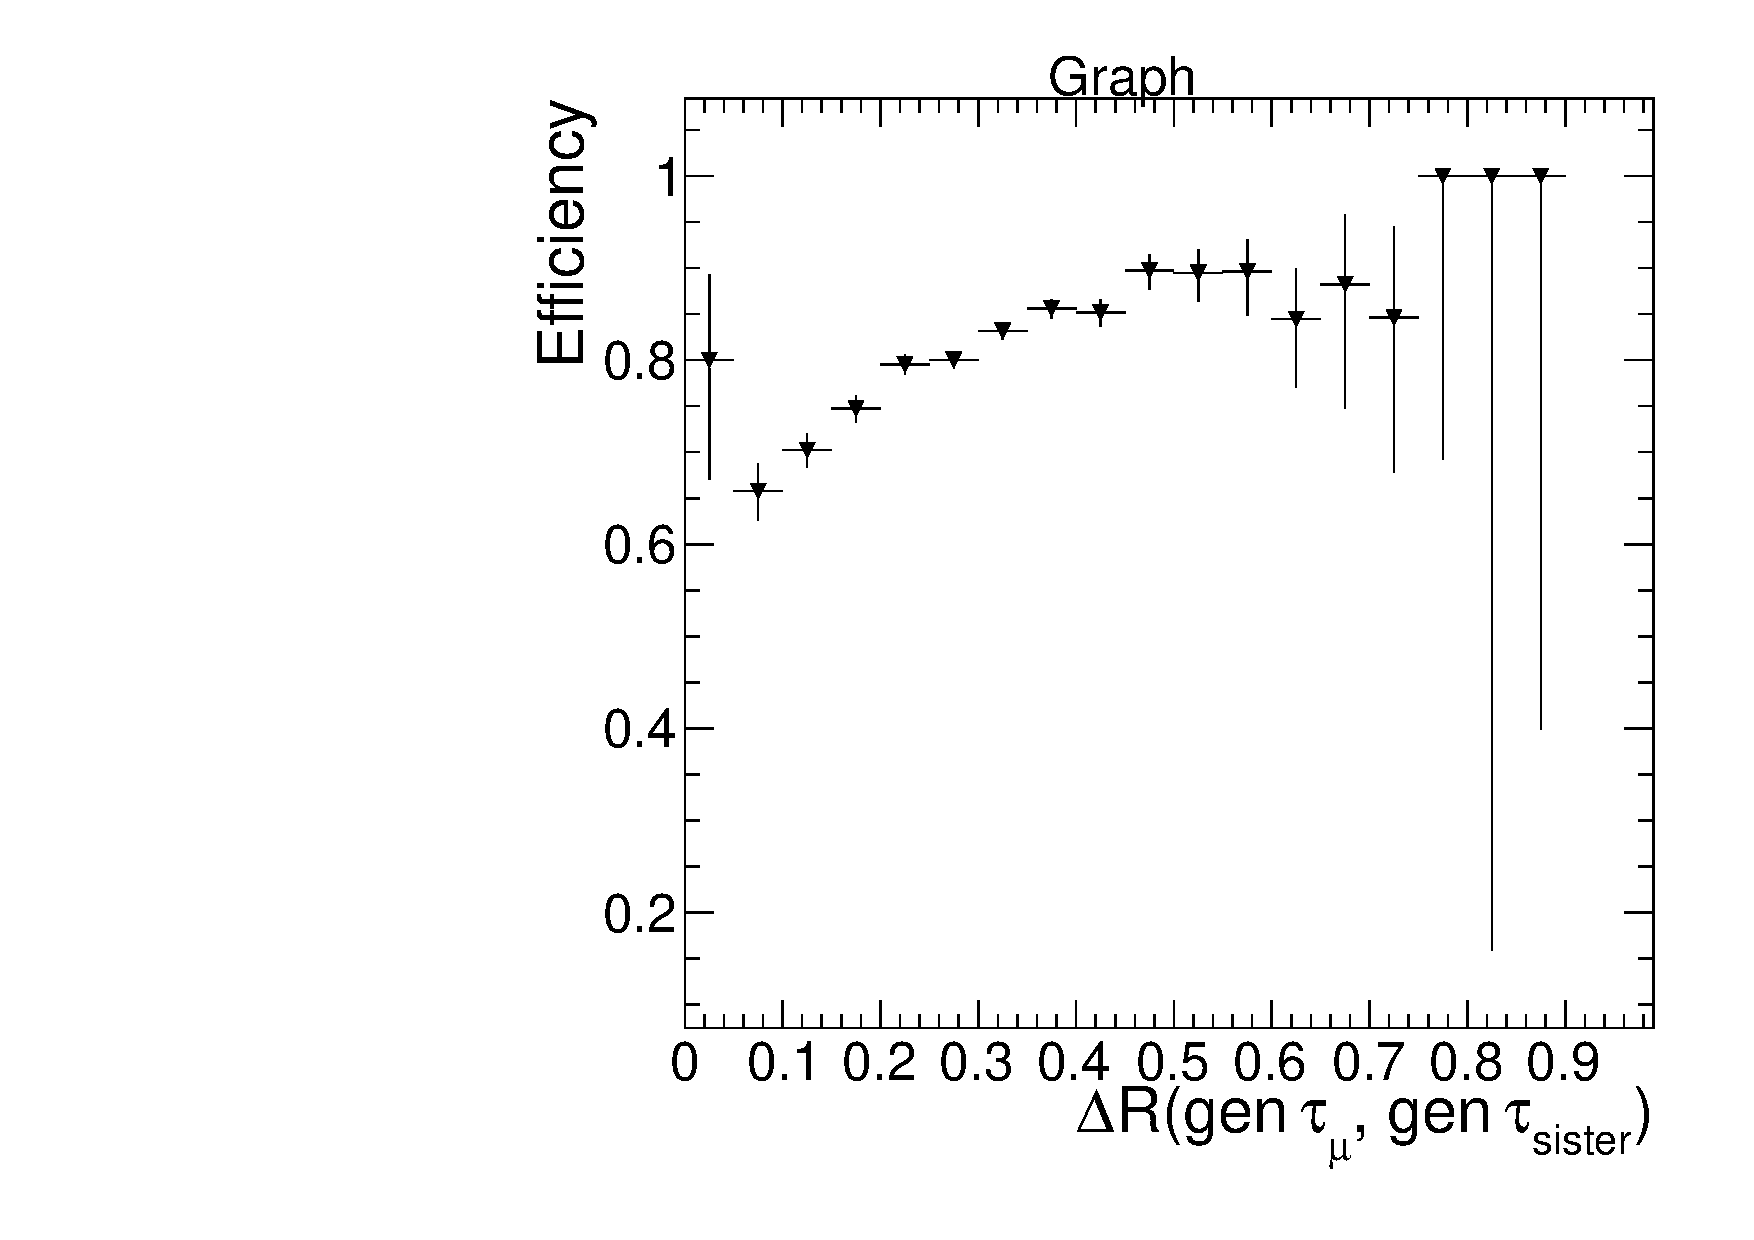
\includegraphics[width=0.8\cmsFigWidth]{figures/dREfficiency_WmuIDIso_muMuOnly}
    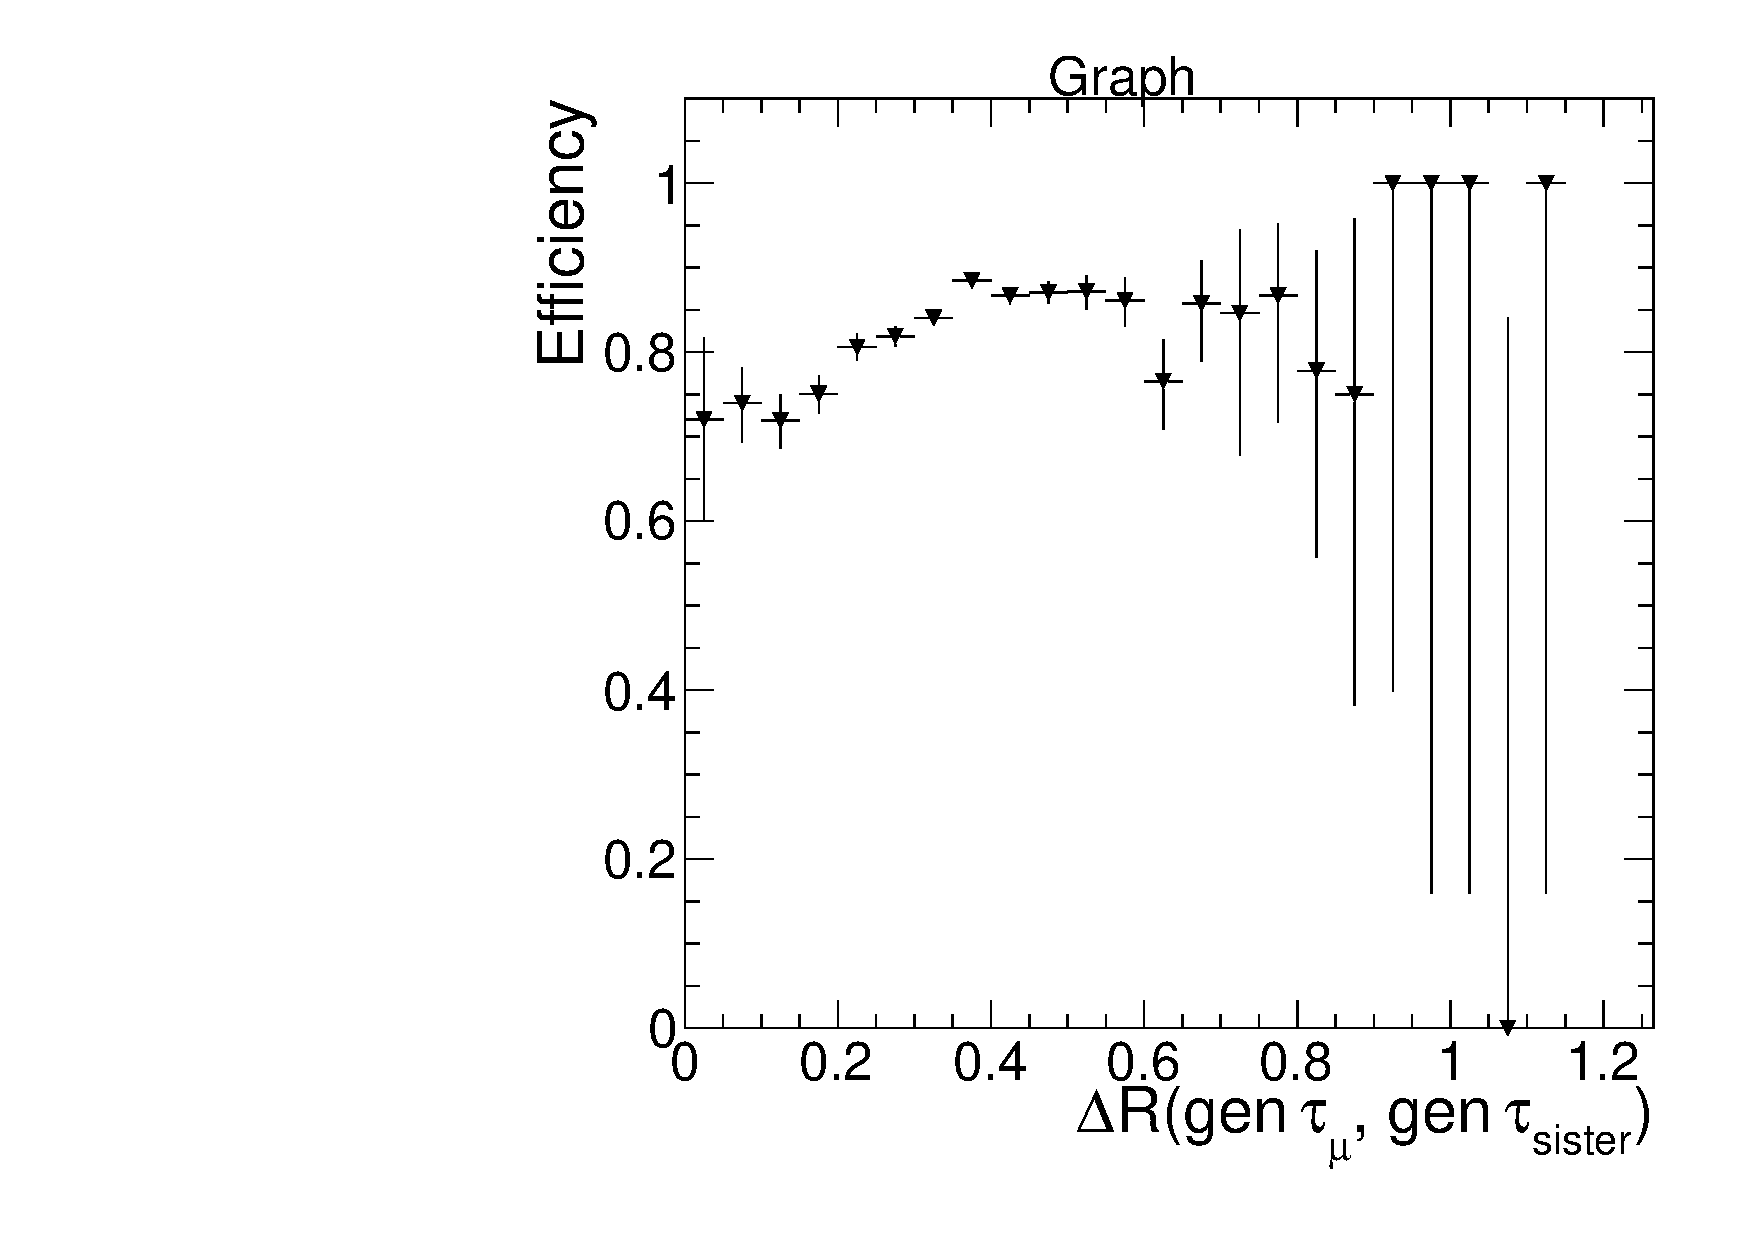
\includegraphics[width=0.8\cmsFigWidth]{figures/dREfficiency_WmuIDIso_muHadOnly}
    \caption{$\epsilon_{\text{HLT}}^{\text{no }l\text{ iso}}$ for the ggH signal as a function of the separation $\Delta$R(gen $a\rightarrow\tau\rightarrow\mu$ muon, gen $\tau_{\text{2}}$), where the gen $\tau_{\text{2}}$ is a decay product of the same pseudoscalar as in the $a\rightarrow\tau\rightarrow\mu$.  The $a\rightarrow\tau\rightarrow\mu$ muon is matched to the reco'd muon as described in the text.  The reco'd muon is required to pass the trigger muon ID of Sec.~\ref{sec:evtsel-triggermu}, but with the nearby lepton isolation requirement removed.  (\cmsLeft) Gen $\tau_{\text{2}}$ decays to an electron.  (middle) Gen $\tau_{\text{2}}$ decays to a muon.  (\cmsRight) Gen $\tau_{\text{2}}$ decays to hadrons.}
    \label{fig:HLTEffVsDR}
  \end{center}
\end{figure}

In contrast, Figure~\ref{fig:HLTEffVsDR_withFilters} shows $\epsilon_{\text{HLT}}$ as a function of $\Delta$R(gen $a\rightarrow\tau\rightarrow\mu$ muon, gen $\tau_{\text{2}}$), where the gen $a\rightarrow\tau\rightarrow\mu$ muon is matched to the reco'd muon as described in Eq.~\ref{eq:muonHLTeff} above and the gen $\tau_{\text{2}}$ is the other tau from the $a\rightarrow\tau\rightarrow\mu$ decay.  The efficiency is calculated separately for each decay mode of the gen $\tau_{\text{2}}$ (electronic, muonic, or hadronic).  The efficiencies are much flatter in $\Delta$R when the nearby lepton isolation requirement is applied to the reconstructed trigger muon, because it ensures that events can pass the selection sequence only if the two reconstructed taus from the pseudoscalar decay are well separated.  The trigger efficiency for $a\rightarrow\tau\rightarrow\mu$ muons in these events is similar to that of $W$ decay muons and is in the regime where the trigger muon is isolated and MC describes the data well.

\begin{figure}[hbtp]
  \begin{center}
    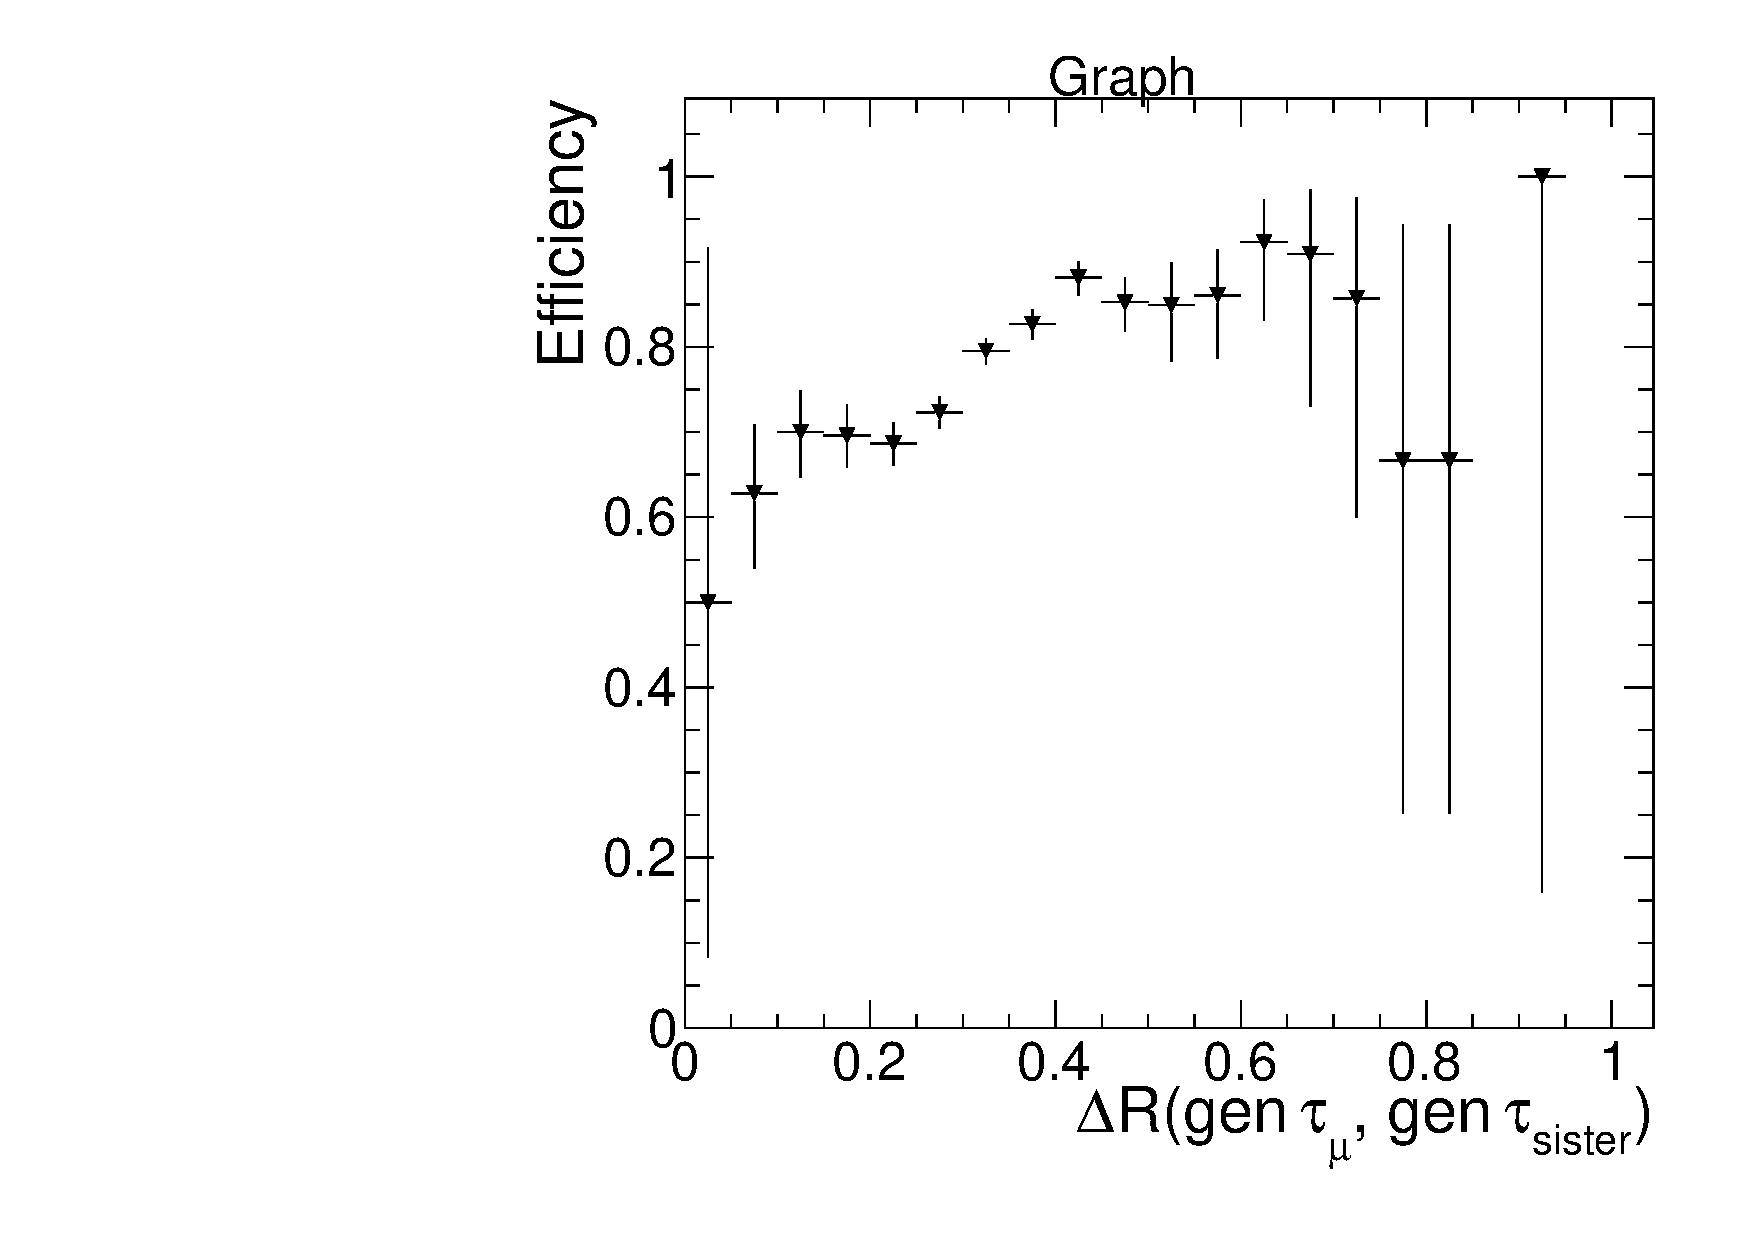
\includegraphics[width=0.8\cmsFigWidth]{figures/dRHLTEfficiency_WmuIDIso_withFilters_muEOnly}
    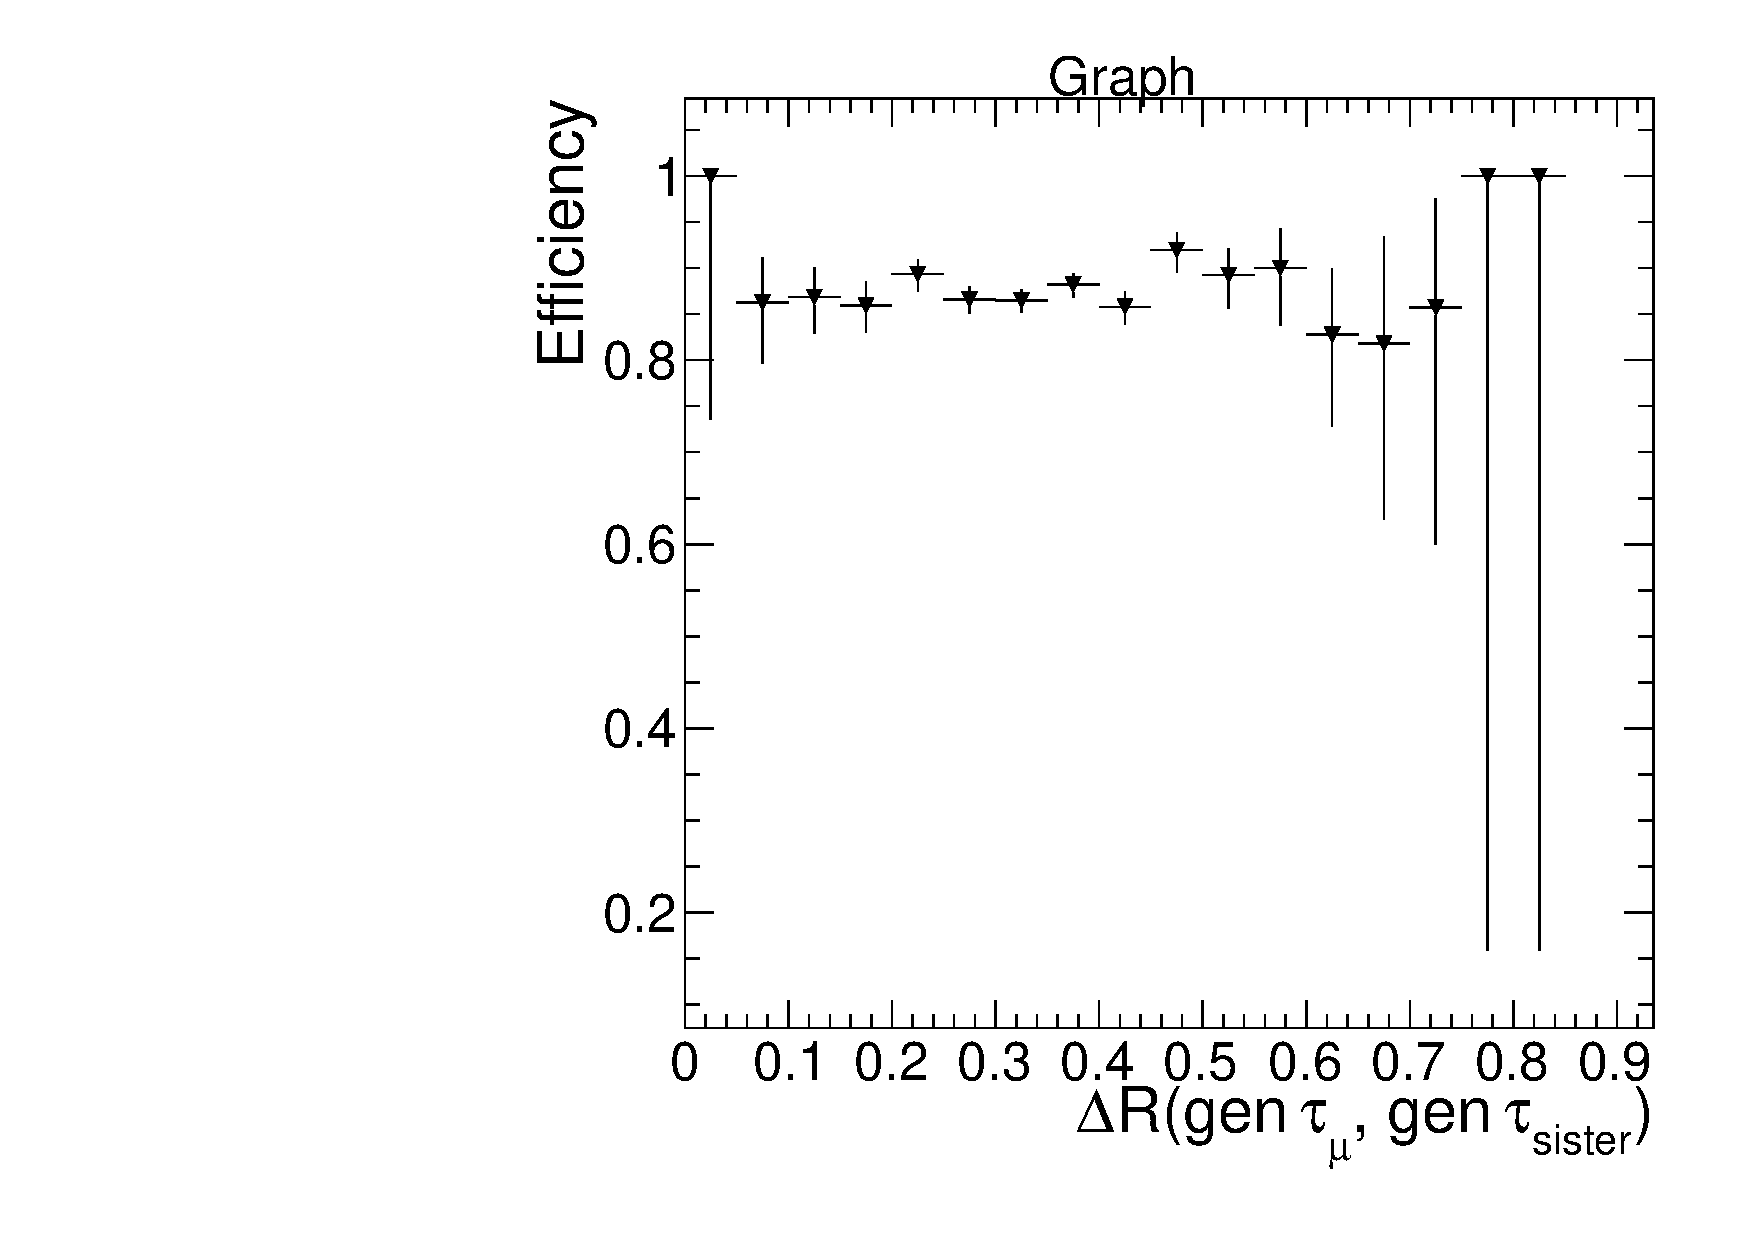
\includegraphics[width=0.8\cmsFigWidth]{figures/dRHLTEfficiency_WmuIDIso_withFilters_muMuOnly}
    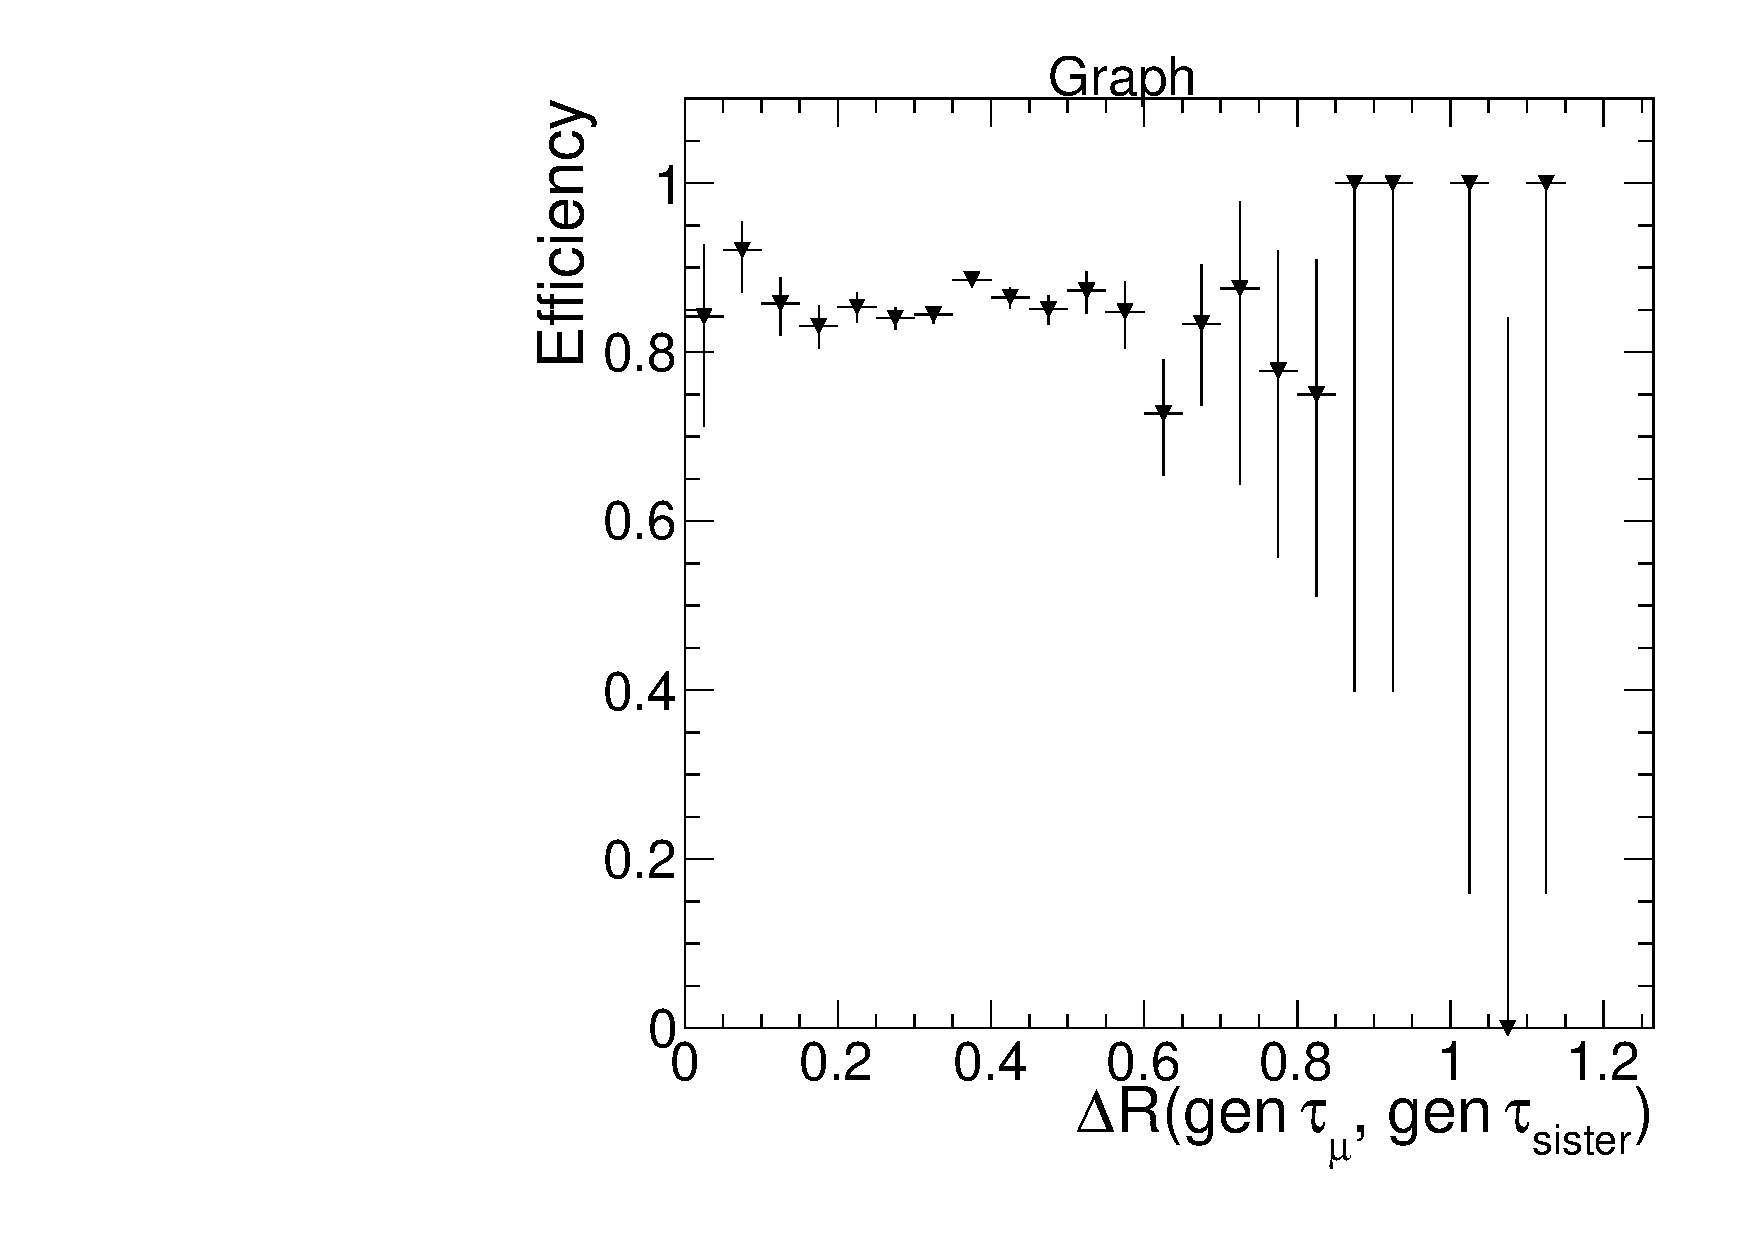
\includegraphics[width=0.8\cmsFigWidth]{figures/dRHLTEfficiency_WmuIDIso_withFilters_muHadOnly}
    \caption{$\epsilon_{\text{HLT}}$ for the ggH signal as a function of the separation $\Delta$R(gen $a\rightarrow\tau\rightarrow\mu$ muon, gen $\tau_{\text{2}}$), where the gen $\tau_{\text{2}}$ is a decay product of the same pseudoscalar as in the $a\rightarrow\tau\rightarrow\mu$.  The $a\rightarrow\tau\rightarrow\mu$ muon is matched to the reco'd muon as described in the text.  The reco'd muon is required to pass the trigger muon ID of Sec.~\ref{sec:evtsel-triggermu}.  (\cmsLeft) Gen $\tau_{\text{2}}$ decays to an electron.  (middle) Gen $\tau_{\text{2}}$ decays to a muon.  (\cmsRight) Gen $\tau_{\text{2}}$ decays to hadrons.}
    \label{fig:HLTEffVsDR_withFilters}
  \end{center}
\end{figure}

Figure~\ref{fig:HLT-eff-W-mu} shows the HLT efficiency for muons passing the trigger muon ID in both the WH and gluon fusion production modes.  In both modes, the trigger muon ID includes the nearby lepton non-overlap requirement.  The efficiencies are very similar for the reasons discussed above.

\begin{figure}[hbtp]
  \begin{center}
    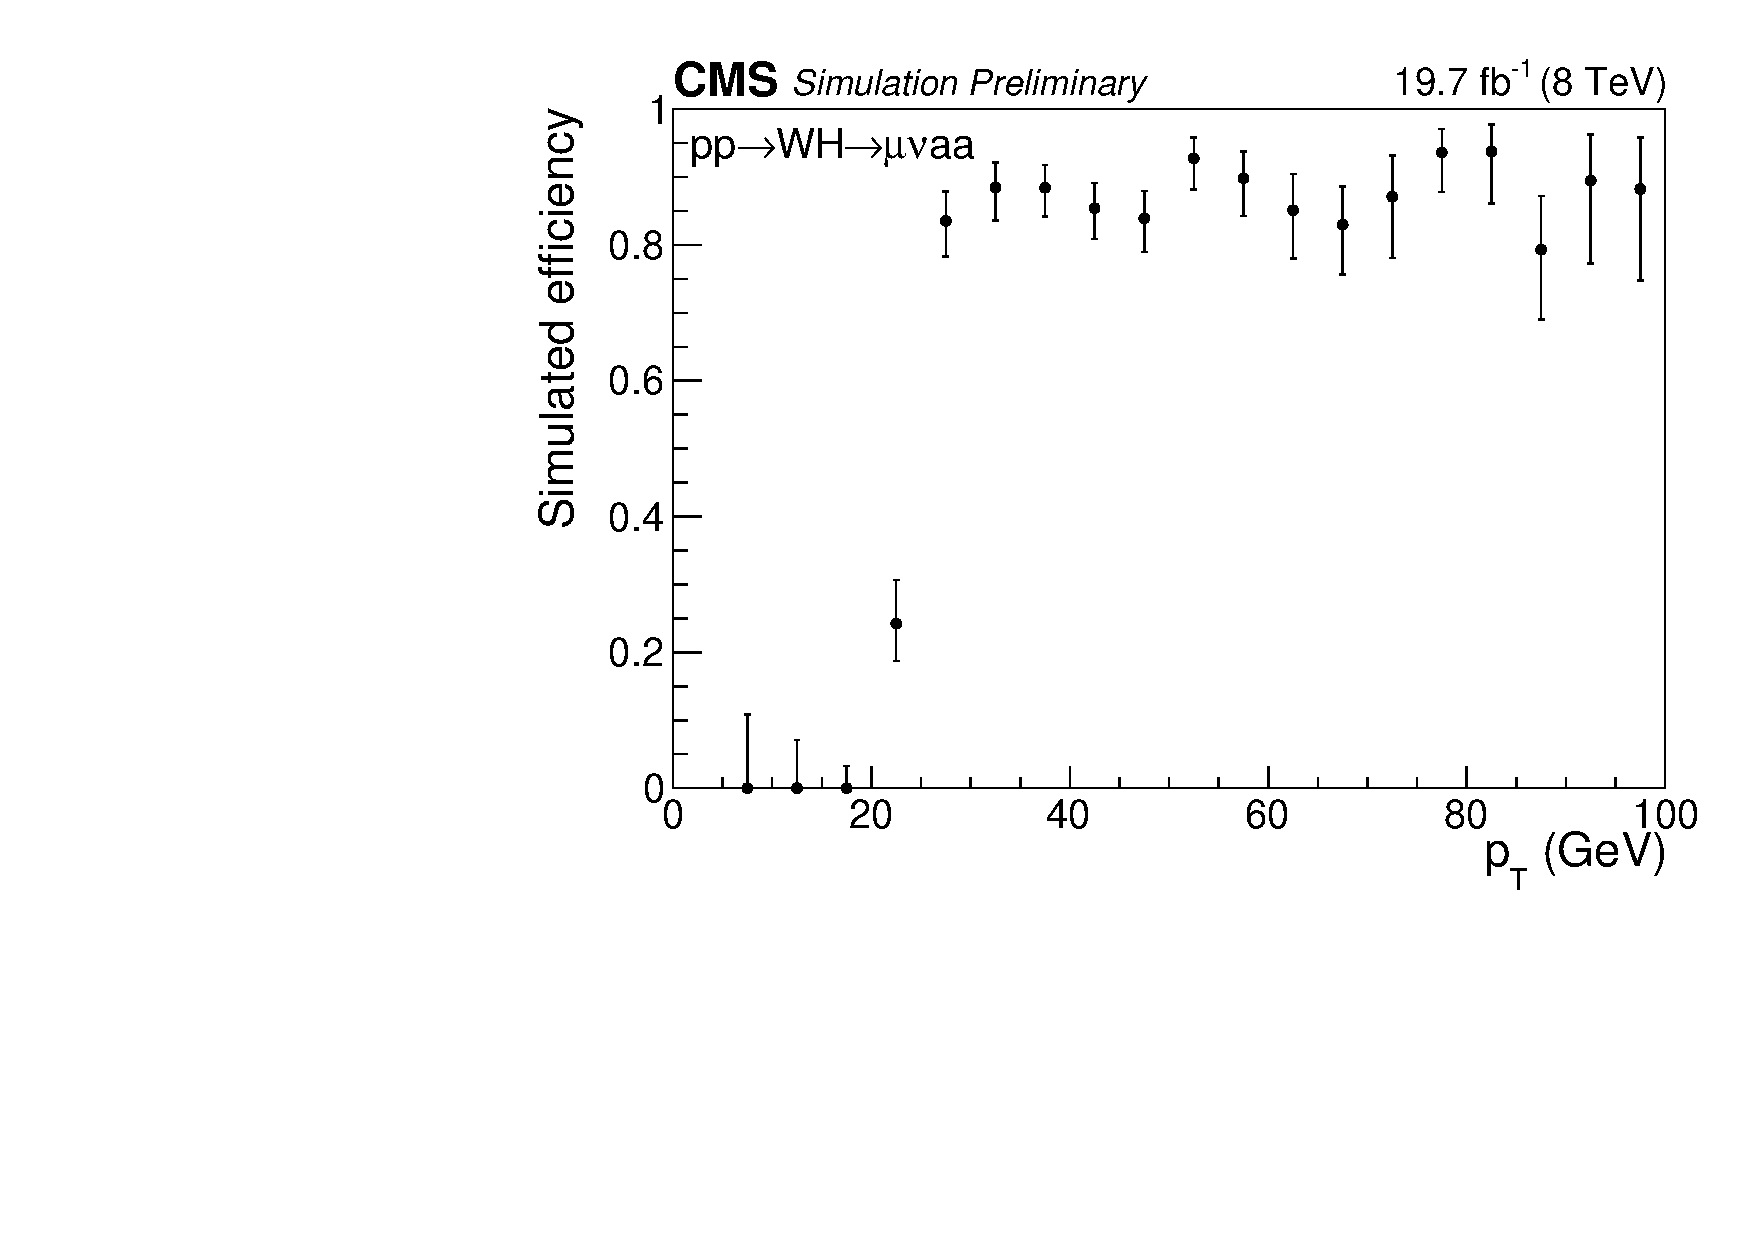
\includegraphics[width=1.24\cmsFigWidth]{figures/HLT_eff_Wmu_WH}
    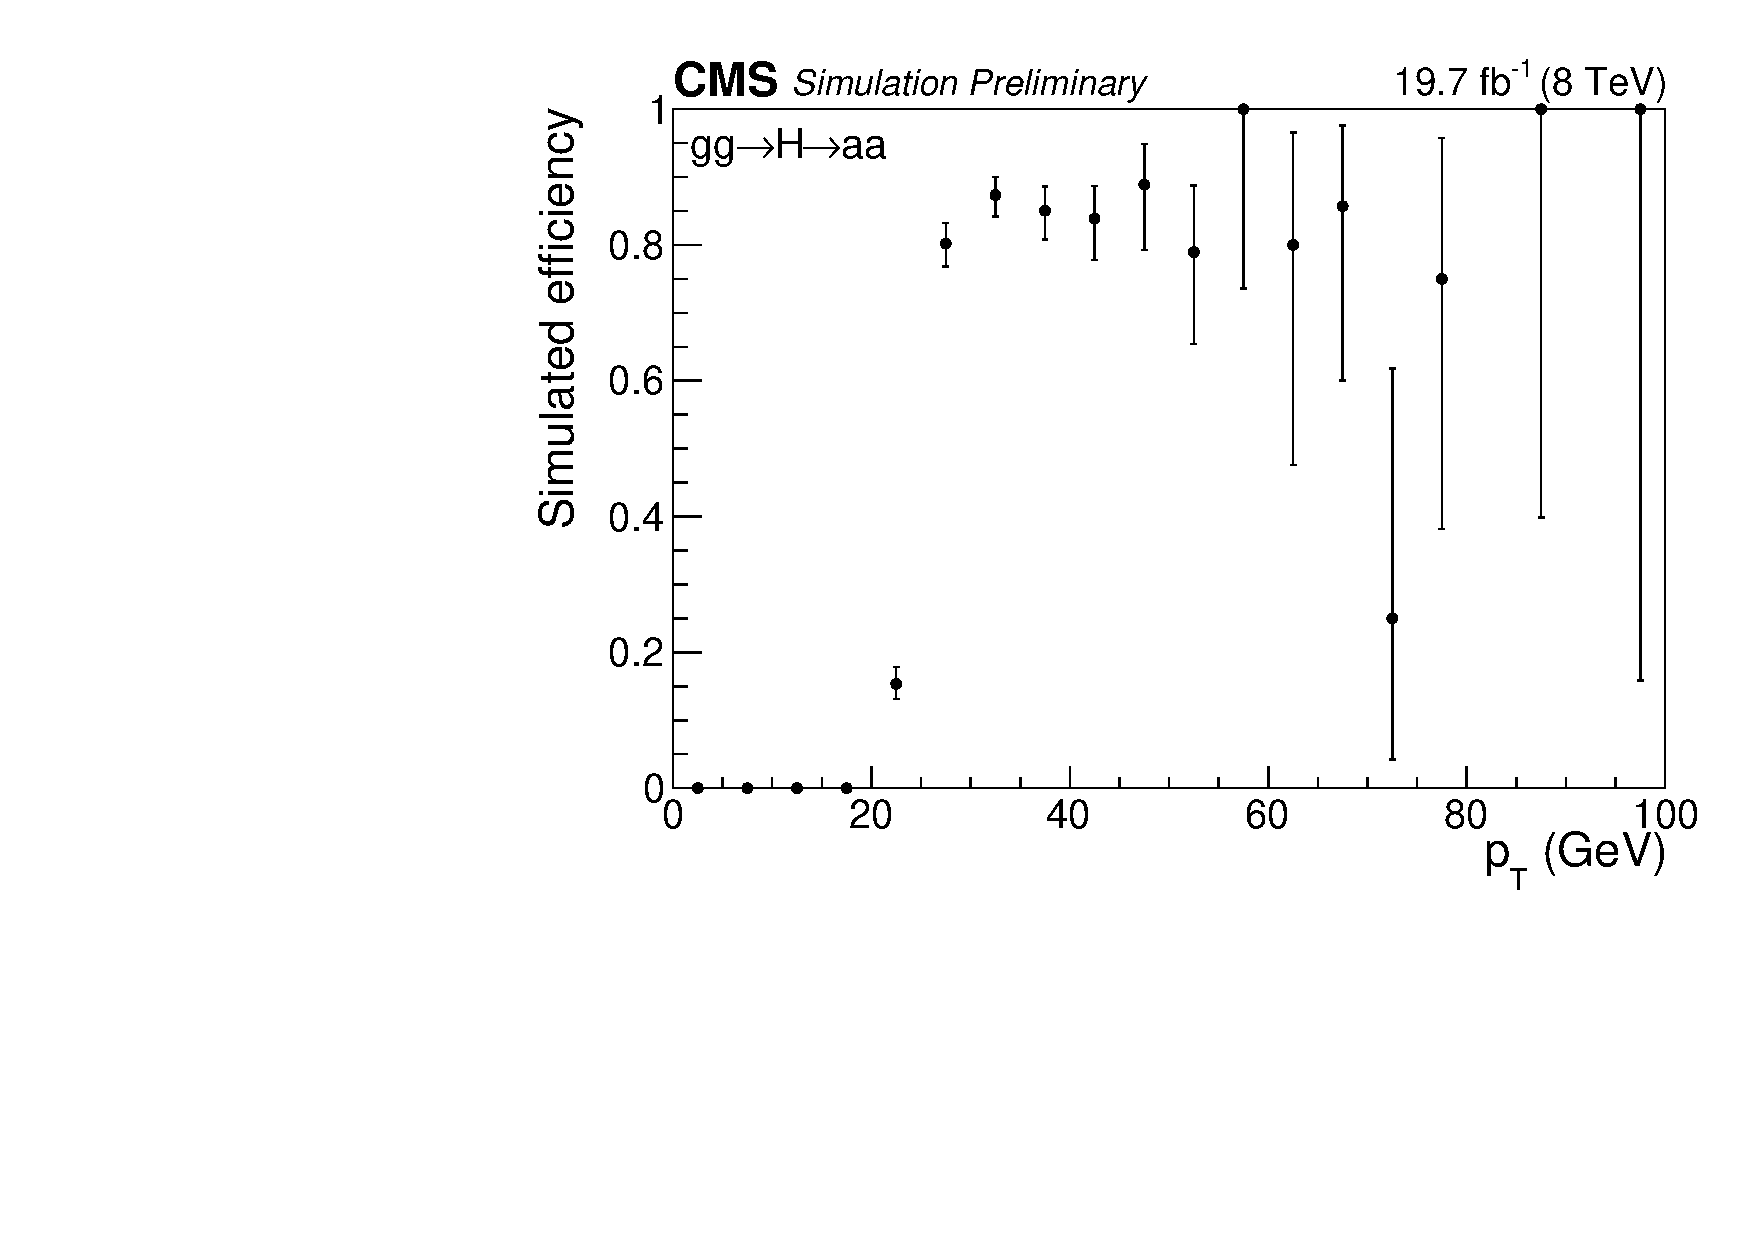
\includegraphics[width=1.24\cmsFigWidth]{figures/HLT_eff_Wmu_ggH}
    \caption{MC simulation prediction of efficiency for reconstructed muons passing the trigger muon ID to fire \texttt{HLT\_IsoMu24\_eta2p1}. Efficiencies were measured in MC events where the Higgs is produced via the (\cmsLeft) WH and (\cmsRight) gluon fusion channels.}
    \label{fig:HLT-eff-W-mu}
  \end{center}
\end{figure}

%Iso efficiency subsection
\subsection{Study of the particle flow relative isolation efficiency for signal events produced via gluon fusion\label{sec:muon-id-eff-iso}}

The efficiency for ggH $a\rightarrow\tau\rightarrow\mu$ decay muons that pass the tight muon ID criteria to pass the PF relative isolation cut is calculated for two reconstructed muon selections.  As a reminder, the PF relative isolation is defined as the $p_T$ sum of all PF hadrons and photons within a cone of $\Delta$R = 0.4 around the trigger muon divided by the trigger muon $p_T$.  Both selections have the PF relative isolation requirement of Sec.~\ref{sec:evtsel-triggermu} removed, since it is the efficiency of that requirement being studied here.   Barring that, the first selection is identical to the criteria described in Sec.~\ref{sec:evtsel-triggermu}, except that in addition the nearby lepton isolation requirement is removed.  Similarly, barring the PF relative isolation requirement, the second selection is identical to the criteria described in Sec.~\ref{sec:evtsel-triggermu}.  PF relative isolation efficiency is compared for the two selections.  Since the signature of pseudoscalar decays in the detector is similar between the ggH and VBF production modes, the results obtained for ggH simulation can be applied to VBF simulation as well.

The PF relative isolation efficiencies of the two selections are given by 

\begin{equation}
\epsilon_{\text{rel. iso}}^{\text{no }l\text{ iso}} = \frac{\text{No. gen-matched reco'd muons passing no-lepton-isolation ID and PF rel. iso.}}{\text{No. gen-matched reco'd muons passing trigger muon ID excl. PF rel. iso.}} \\
\label{eq:muonPFRelIsoeff-noliso}
\end{equation}

\begin{equation}
\epsilon_{\text{rel. iso.}} = \frac{\text{No. gen-matched reco'd muons passing trigger muon ID incl. PF. rel. iso.}}{\text{No. gen-matched reco'd muons passing trigger muon ID excl. PF rel. iso.}} \\
\label{eq:muonPFRelIsoeff}
\end{equation}

where

\begin{itemize}
\item the gen-matching criteria is $\Delta$$p_T$(reco muon, gen $a\rightarrow\tau\rightarrow\mu$ muon) $<$ 0.1 GeV and the gen muon is from the decay of a tau that is itself from the decay of a pseudoscalar;
\item the trigger muon ID for $\epsilon_{\text{rel. iso.}}^{\text{no }l\text{ iso}}$ is as described in Sec.~\ref{sec:evtsel-triggermu} but with the PF relative isolation and nearby lepton isolation requirements removed;
\item the trigger muon ID for $\epsilon_{\text{rel. iso.}}$ is as described in Sec.~\ref{sec:evtsel-triggermu} but with the PF relative isolation requirement removed; and
\item ``rel. iso.'' refers to passing the cut PF relative isolation $<$ 0.12.
\end{itemize}

Figure~\ref{fig:IsoEffVsDR} shows $\epsilon_{\text{rel. iso.}}^{\text{no }l\text{ iso}}$ as a function of $\Delta$R(gen $a\rightarrow\tau\rightarrow\mu$ muon, gen $\tau_{\text{2}}$), where the gen $a\rightarrow\tau\rightarrow\mu$ muon is matched to the reco'd muon as described in Eq.~\ref{eq:muonPFRelIsoeff-noliso} above and the gen $\tau_{\text{2}}$ is the other tau from the $a\rightarrow\tau\tau$ decay.  The efficiency is calculated separately for each decay mode of the gen $\tau_{\text{2}}$ (electronic, muonic, or hadronic).  $\epsilon_{\text{rel. iso.}}^{\text{no }l\text{ iso}}$ is $\sim$80\%, independent of $\Delta$R, for the $\tau_{\mu}\tau_{\text{e}}$ the $\tau_{\mu}\tau_{\mu}$ channels.  Because PF electrons and muons are not counted in the PF relative isolation sum, the presence of a nearby $\tau_{\text{e}}$ or $\tau_{\mu}$ does not significantly spoil the relative isolation of the main $a\rightarrow\tau\rightarrow\mu$ muon.  The overall efficiency is lower than the efficiency for $Z$ decay muons~\cite{1748-0221-7-10-P10002} by $\sim$15\% due to the different kinematics of di-tau objects vs. isolated $Z$ decay muons.  Conversely, in the $\tau_{\mu}\tau_{\text{had}}$ channel, $\epsilon_{\text{rel. iso.}}^{\text{no }l\text{ iso}}$ is $\sim$80\% only for $\Delta$R $>$ 0.4, when the two taus from pseudoscalar decay are separated enough that the tau decay muon appears isolated.  When the two taus are closer than $\Delta$R $\sim$ 0.4, the efficiency decreases because the hadronically decaying non-identified partner tau spoils the relative isolation of the tau decay muon that is identified as a trigger muon.

\begin{figure}[hbtp]
  \begin{center}
    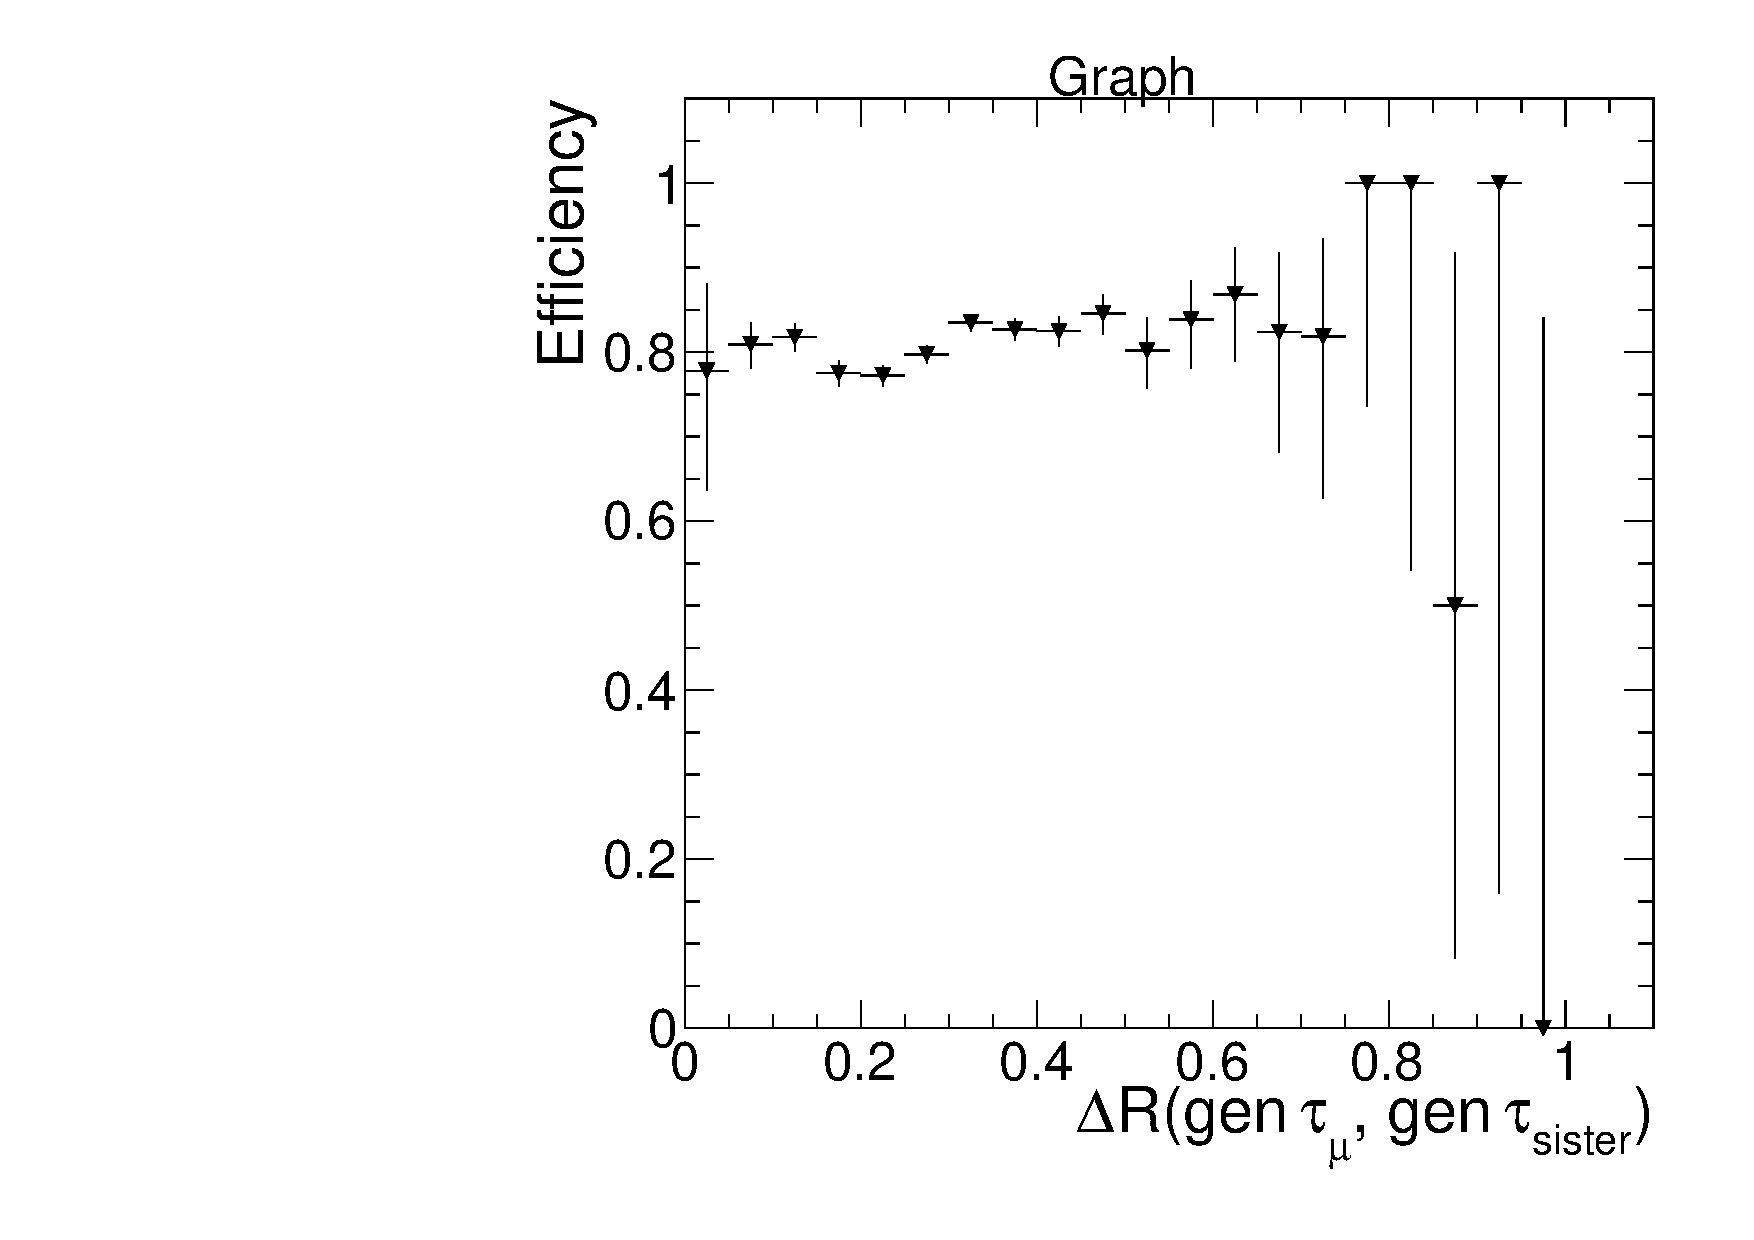
\includegraphics[width=0.8\cmsFigWidth]{figures/dRIsoEfficiency_muEOnly}
    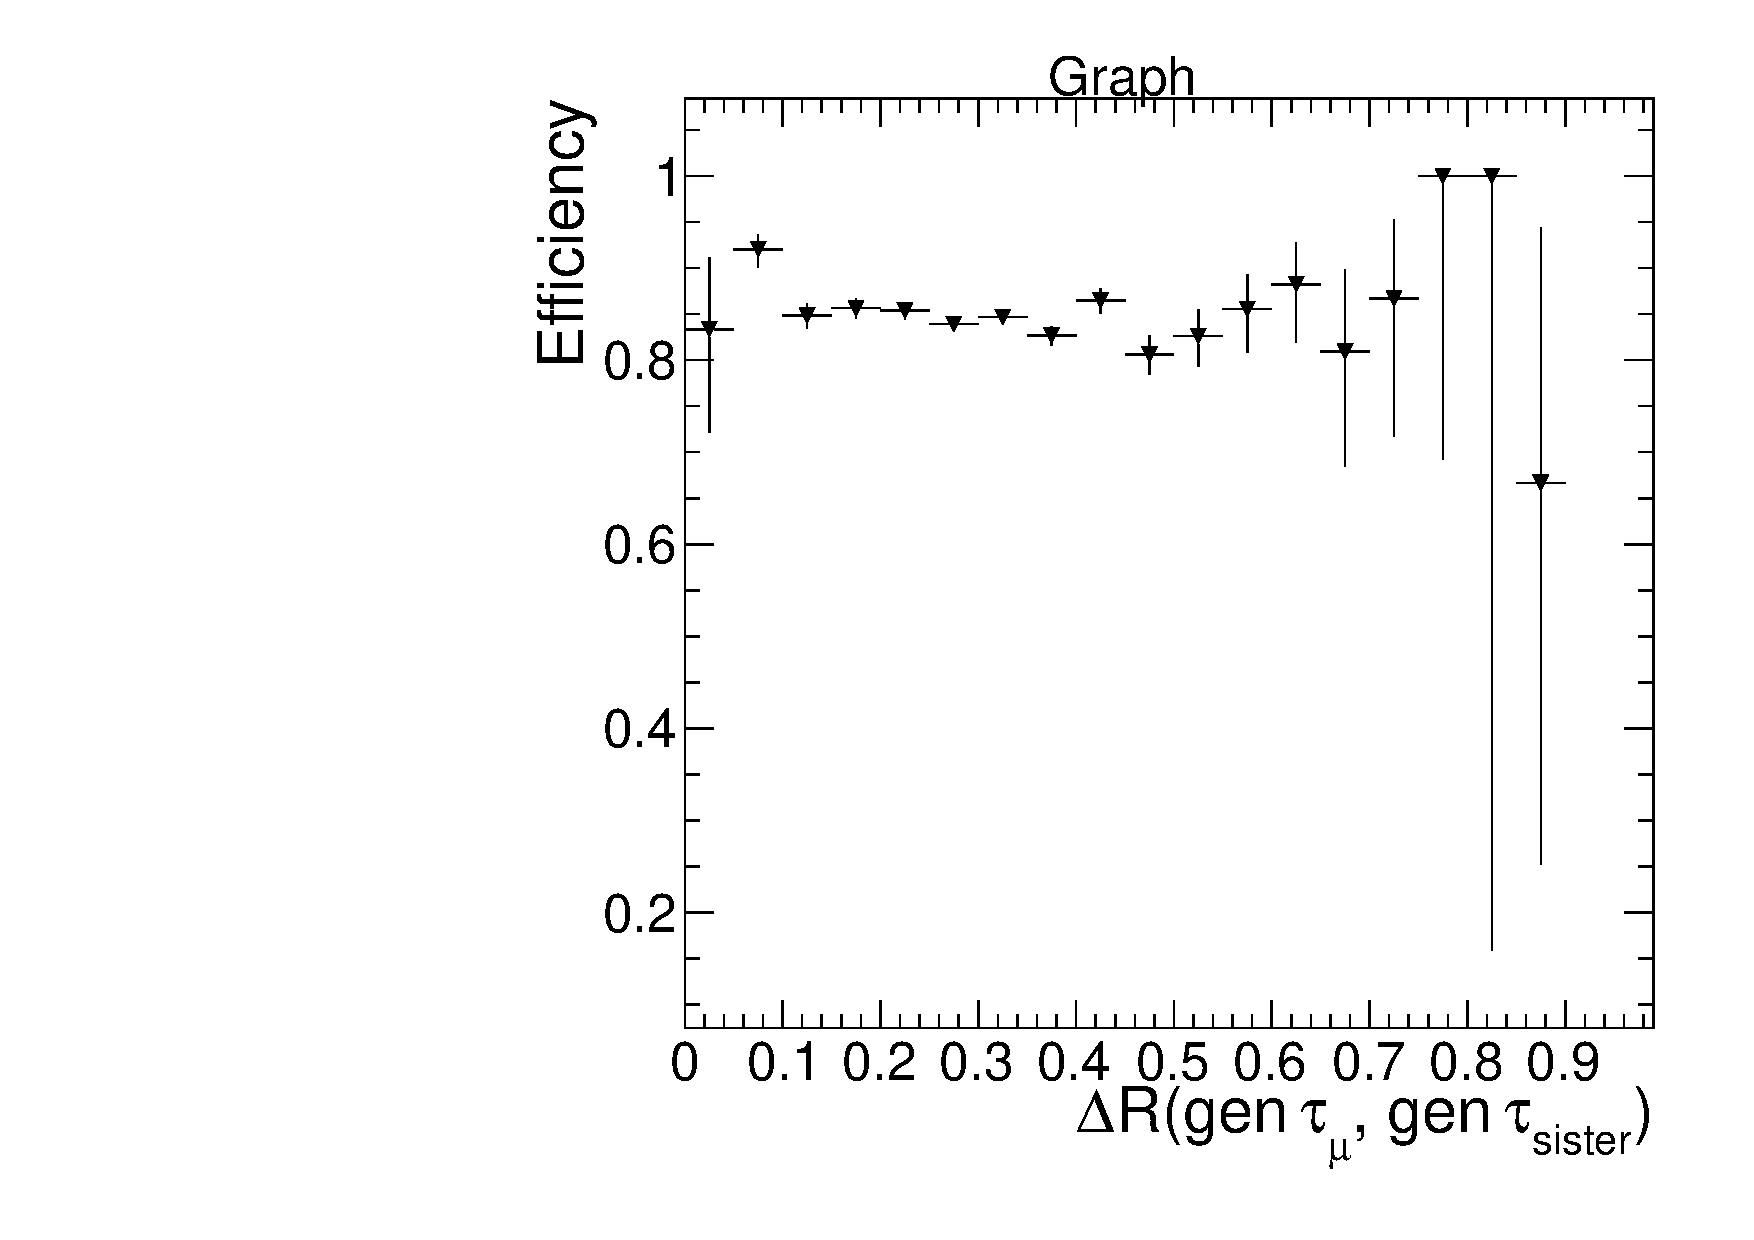
\includegraphics[width=0.8\cmsFigWidth]{figures/dRIsoEfficiency_muMuOnly}
    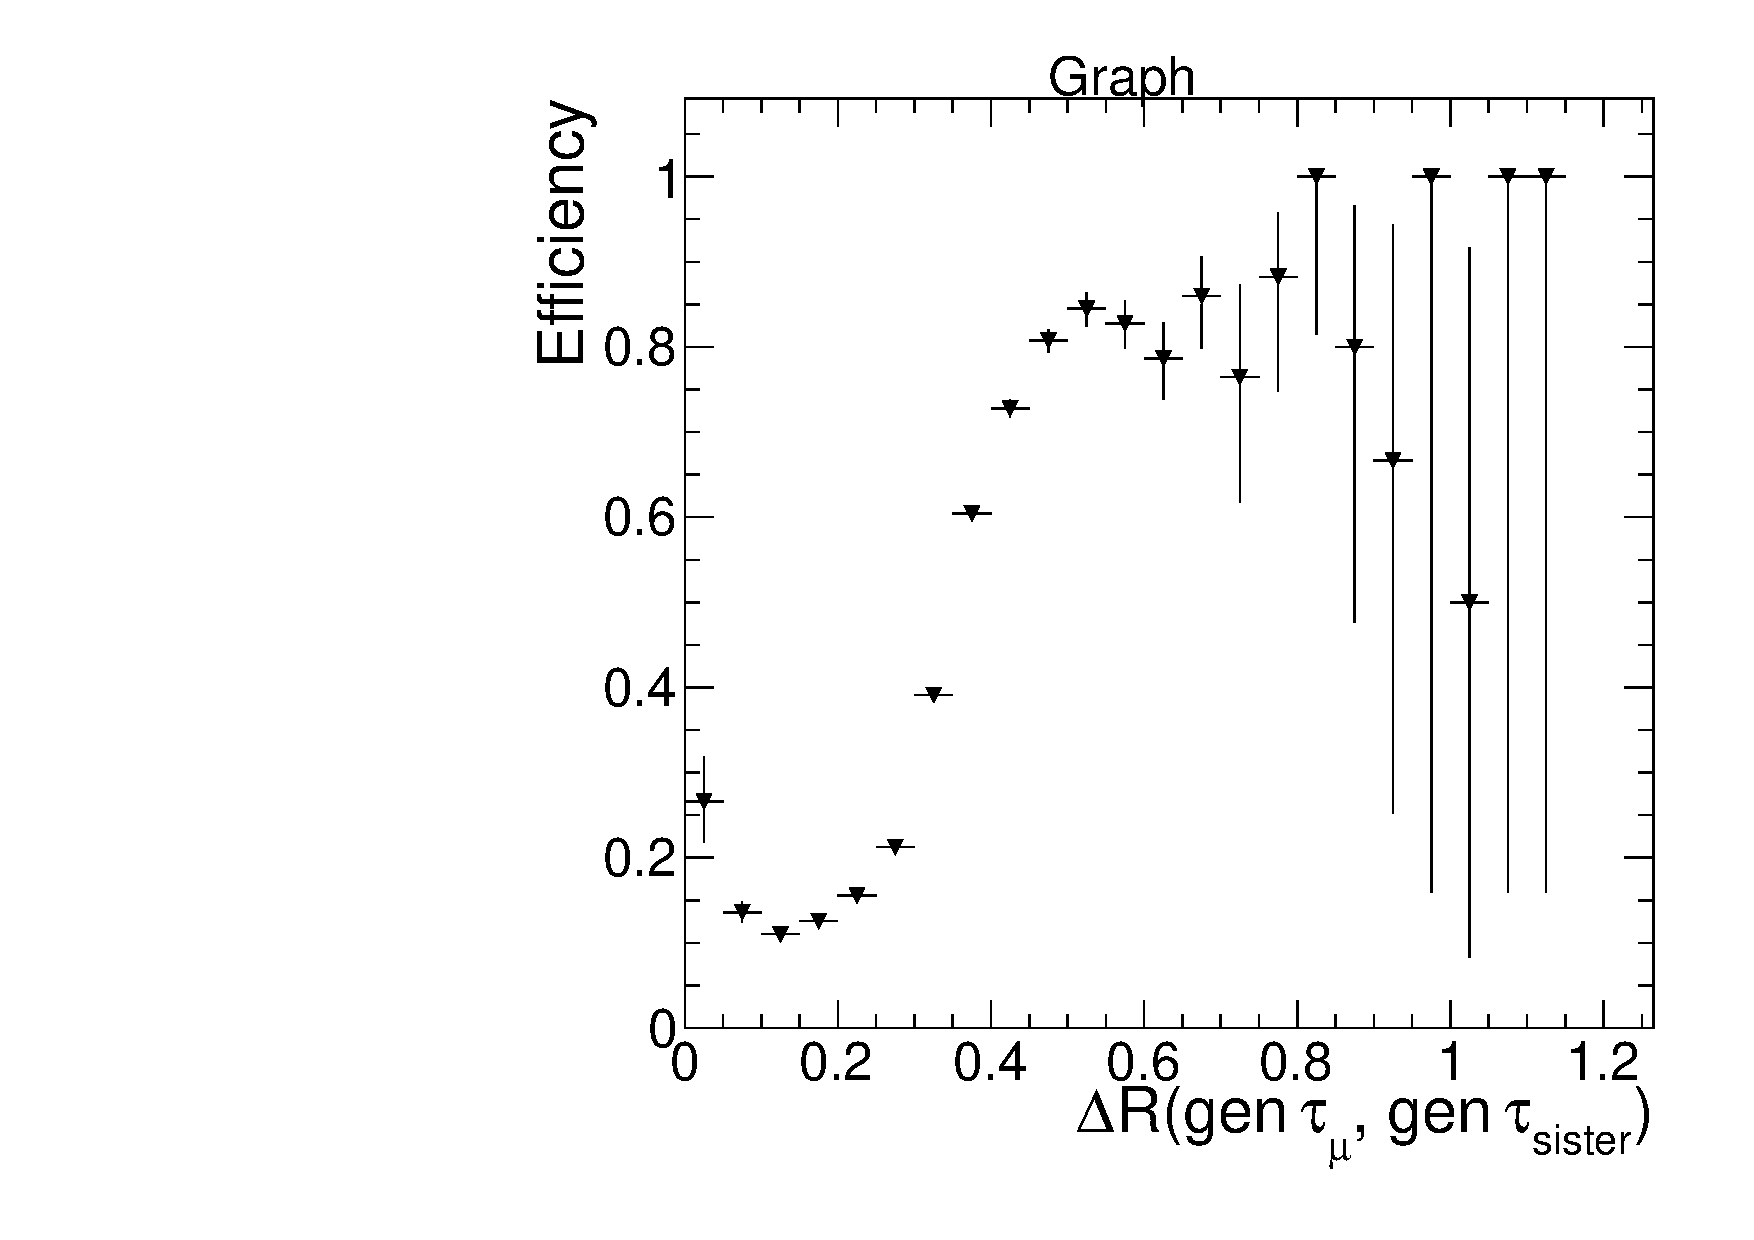
\includegraphics[width=0.8\cmsFigWidth]{figures/dRIsoEfficiency_muHadOnly}
    \caption{$\epsilon_{\text{rel. iso.}}^{\text{no }l\text{ iso}}$ for the ggH signal as a function of the separation $\Delta$R(gen $a\rightarrow\tau\rightarrow\mu$ muon, gen $\tau_{\text{2}}$), where the gen $\tau_{\text{2}}$ is a decay product of the same pseudoscalar as in the $a\rightarrow\tau\rightarrow\mu$.  The $a\rightarrow\tau\rightarrow\mu$ muon is matched to the reco'd muon as described in the text.  The reco'd muon is required to pass the trigger muon ID of Sec.~\ref{sec:evtsel-triggermu}, but with the PF relative isolation (because this is the cut under study) and nearby lepton isolation requirements removed.  (\cmsLeft) Gen $\tau_{\text{2}}$ decays to an electron.  (middle) Gen $\tau_{\text{2}}$ decays to a muon.  (\cmsRight) Gen $\tau_{\text{2}}$ decays to hadrons.}
    \label{fig:IsoEffVsDR}
  \end{center}
\end{figure}

In contrast, Figure~\ref{fig:IsoEffVsDR_withFilters} shows $\epsilon_{\text{rel. iso.}}$ as a function of $\Delta$R(gen $a\rightarrow\tau\rightarrow\mu$ muon, gen $\tau_{\text{2}}$), where the gen $a\rightarrow\tau\rightarrow\mu$ muon is matched to the reco'd muon as described in Eq.~\ref{eq:muonPFRelIsoeff} above and the gen $\tau_{\text{2}}$ is the other tau from the $\cmsSymbolFace{a}\rightarrow\tau\tau$ decay.  The efficiency is calculated separately for each decay mode of the gen $\tau_{\text{2}}$ (electronic, muonic, or hadronic).  The efficiencies are much flatter in $\Delta$R\ when the nearby lepton isolation requirement is applied to the reconstructed trigger muon, because it ensures that events can pass the selection sequence only if the two reconstructed taus from the pseudoscalar decay are well separated.  The PF relative isolation efficiency for $a\rightarrow\tau\rightarrow\mu$ muons in these events is now similar to that of $Z$ decay muons and is in the regime where the trigger muon is isolated and MC describes the data well.

\begin{figure}[hbtp]
  \begin{center}
    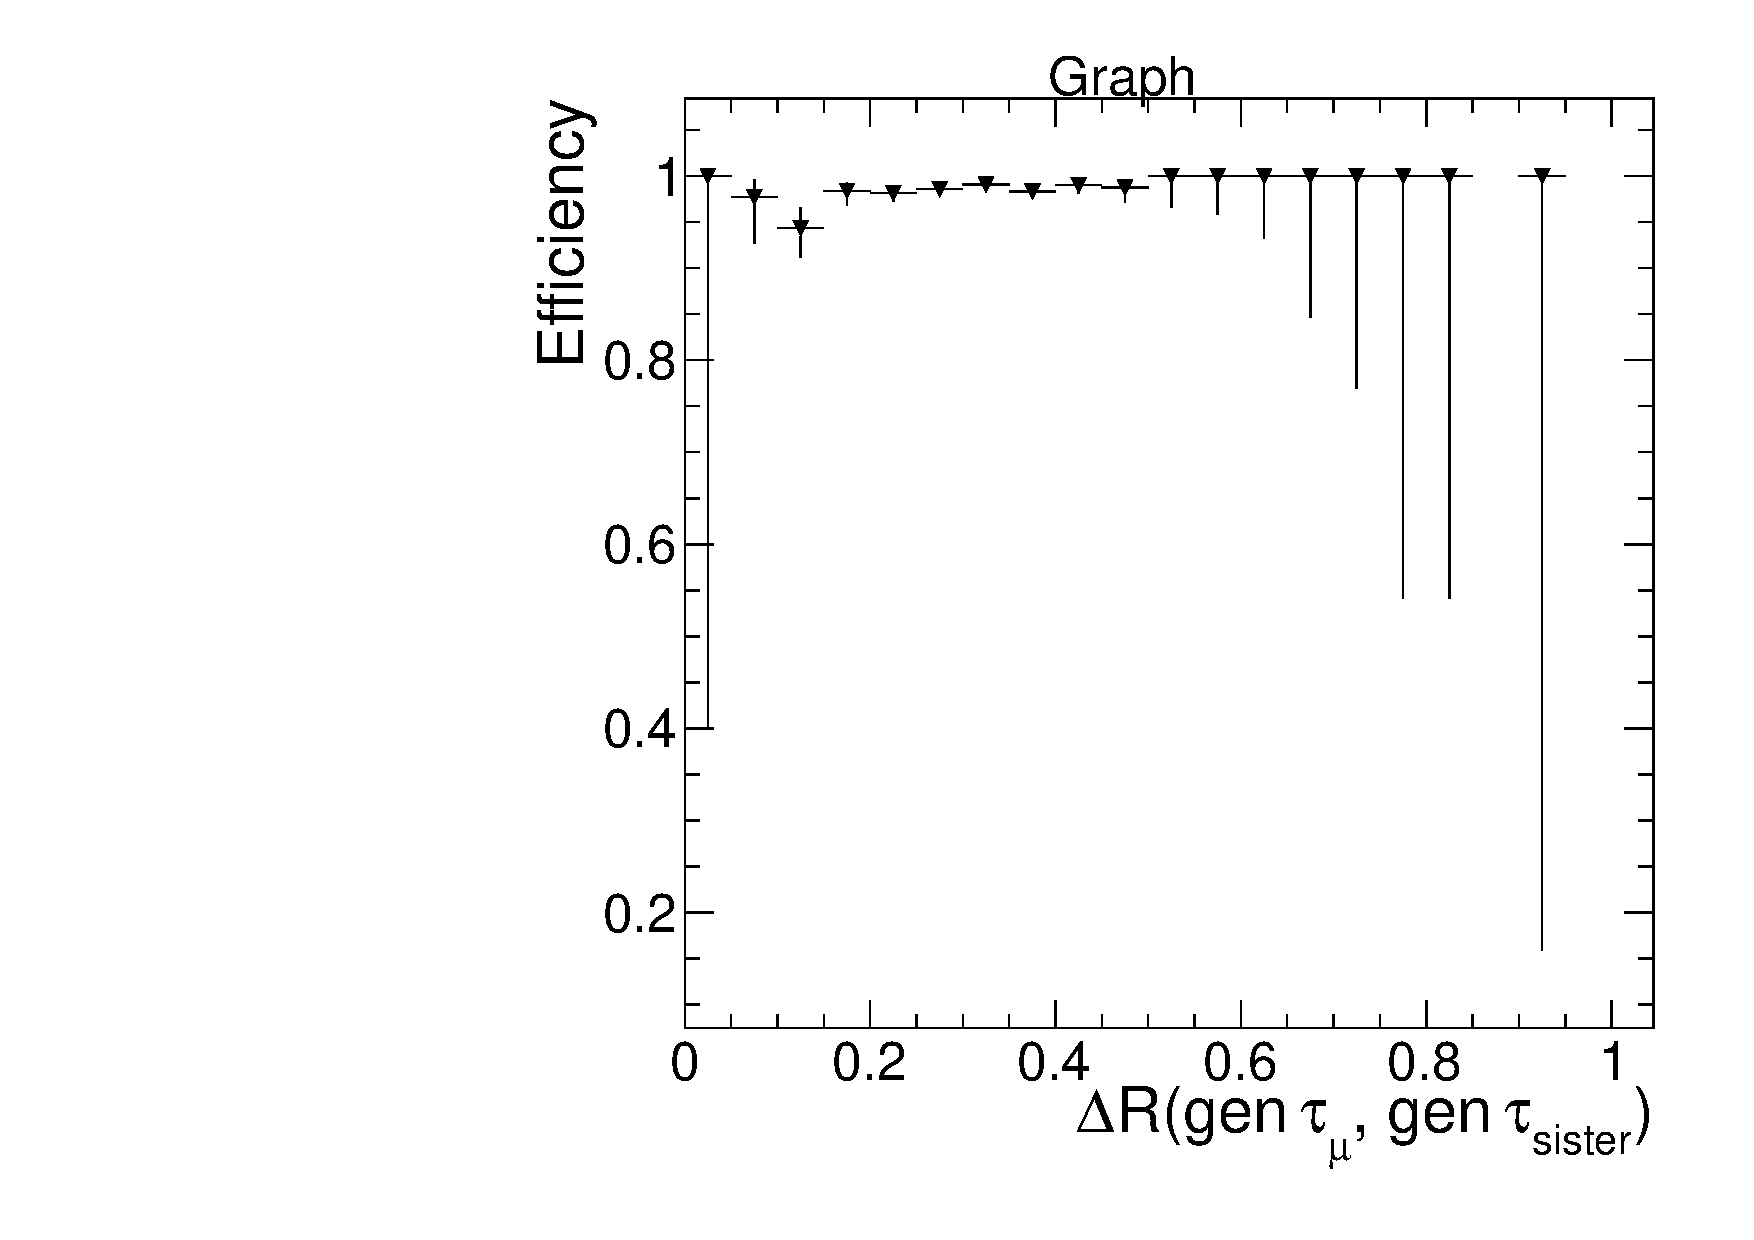
\includegraphics[width=0.8\cmsFigWidth]{figures/dRIsoEfficiency_withFilters_muEOnly}
    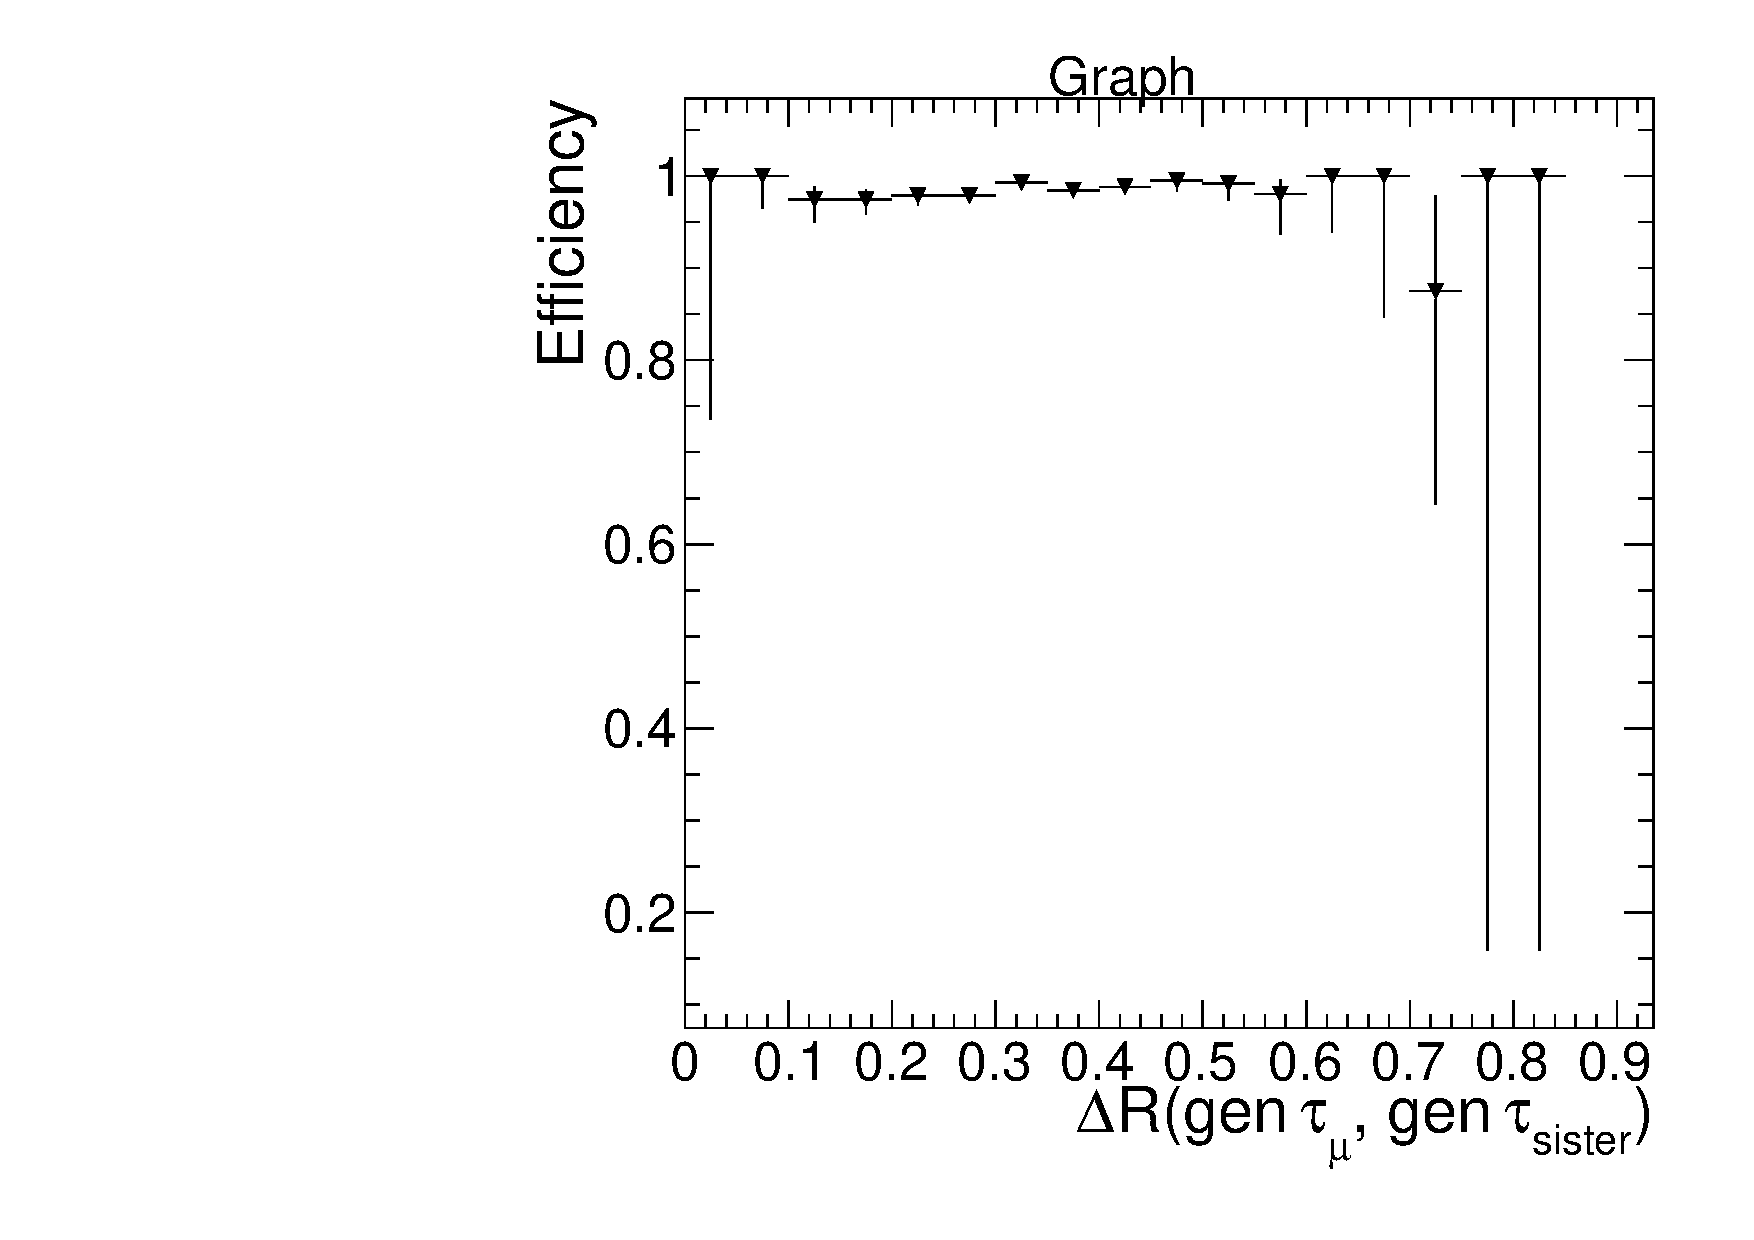
\includegraphics[width=0.8\cmsFigWidth]{figures/dRIsoEfficiency_withFilters_muMuOnly}
    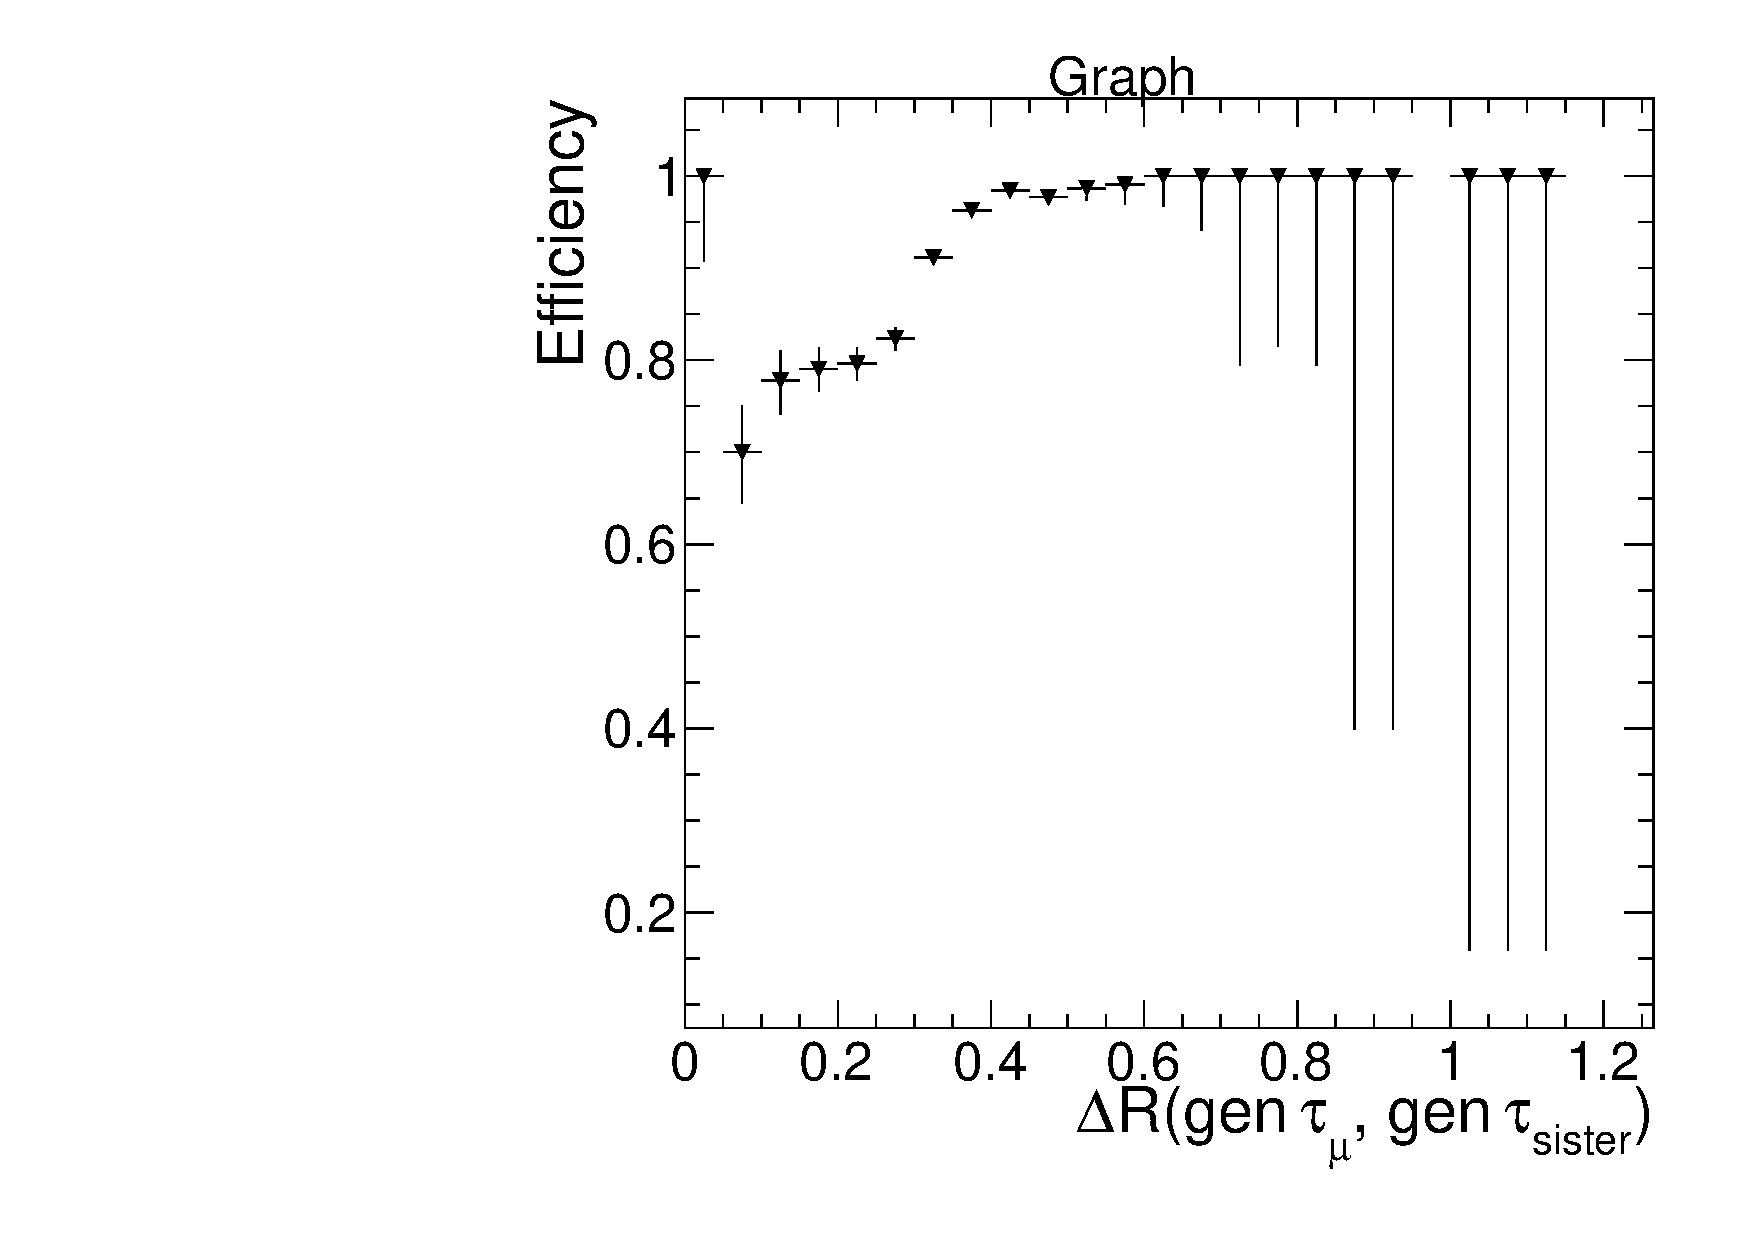
\includegraphics[width=0.8\cmsFigWidth]{figures/dRIsoEfficiency_withFilters_muHadOnly}
    \caption{$\epsilon_{\text{rel. iso.}}$ for the ggH signal as a function of the separation $\Delta$R(gen $a\rightarrow\tau\rightarrow\mu$ muon, gen $\tau_{\text{2}}$), where the gen $\tau_{\text{2}}$ is a decay product of the same pseudoscalar as in the $a\rightarrow\tau\rightarrow\mu$.  The $a\rightarrow\tau\rightarrow\mu$ muon is matched to the reco'd muon as described in the text.  The reco'd muon is required to pass the trigger muon ID of Sec.~\ref{sec:evtsel-triggermu}, but with the PF relative isolation requirement removed (because this is the cut under study).  (\cmsLeft) Gen $\tau_{\text{2}}$ decays to an electron.  (middle) Gen $\tau_{\text{2}}$ decays to a muon.  (\cmsRight) Gen $\tau_{\text{2}}$ decays to hadrons.}
    \label{fig:IsoEffVsDR_withFilters}
  \end{center}
\end{figure}

After all other selection cuts, the acceptance of the nearby lepton isolation requirement ranges from 87\% to 95\% for ggH pseudoscalar masses 7, 9, 11, 13, and 15 GeV.

%boosted tau ID
\section{Boosted tau ID\label{sec:evtsel-ditau}}

The target signature in this search is one in which one of the $a$ decays results in a $\tau_{\mu}\tau_{\text{had}}$ final state, while no constraints are placed on the decay of the taus coming from the other $\cmsSymbolFace{a}$. The hadronic tau identification algorithm employed in this search is the HPS algorithm.

As described in Section~\ref{sec:semileptonic}, the tau pairs produced in the pseudoscalar decays will be highly collimated, and their decay products will invade one another's isolation cones. In particular, for the $\tau_{\mu}\tau_{\text{had}}$ pair, the muon from $\tau_{\mu}$ has been found to end up frequently among the constituents of the jet seeded by the $\tau_{\text{had}}$ decay and therefore among the isolation constituents of the $\tau_{\text{had}}$ reconstructed with HPS.  Figure~\ref{fig:evt-sel-HPS-iso-eff-standard-vs-boosted-ID} shows the $\tau_{\text{had}}$ isolation efficiency for the standard HPS ID versus the boosted $\tau_{\mu}\tau_{\text{had}}$ ID described below.  The isolation efficiency is about four times higher for the boosted $\tau_{\mu}\tau_{\text{had}}$ ID.

\begin{figure}[hbtp]
  \begin{center}
    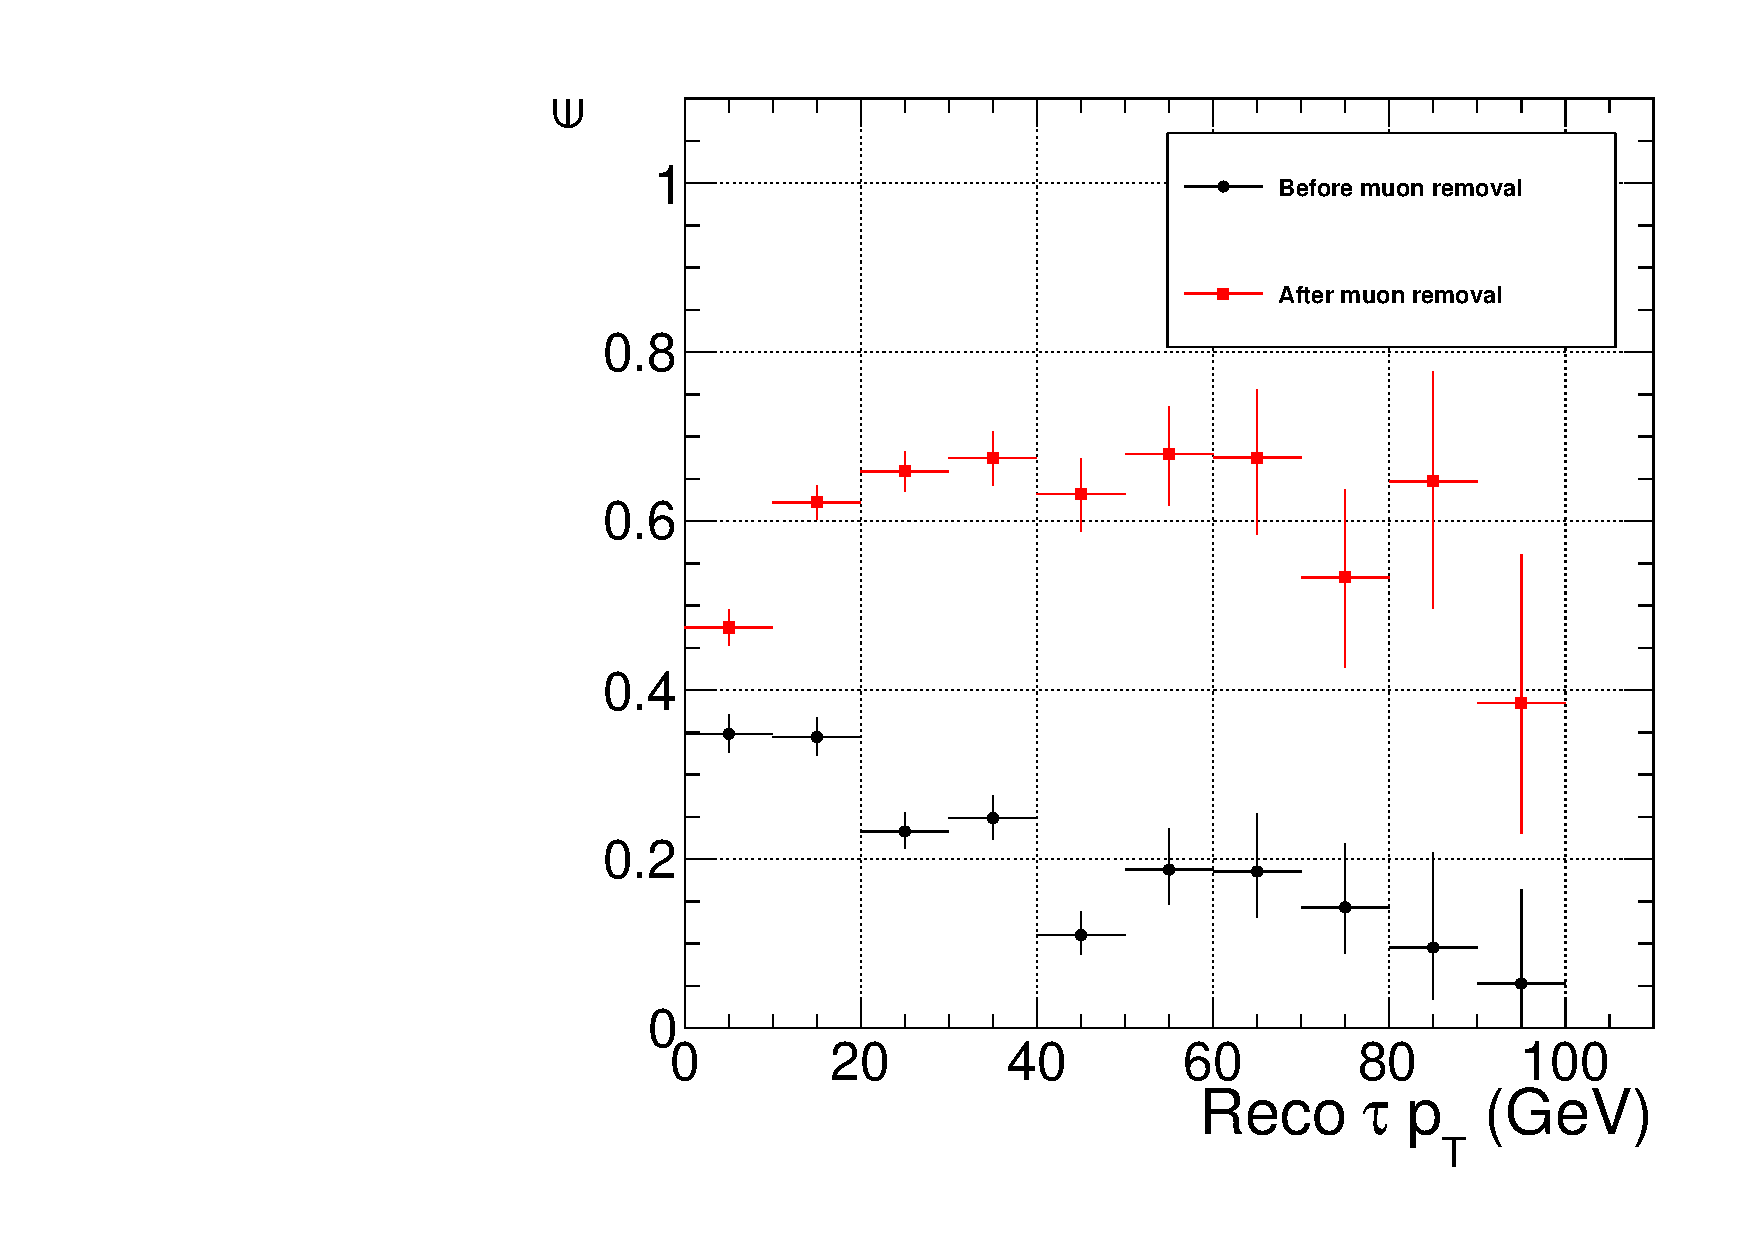
\includegraphics[width=\cmsFigWidth]{figures/effVsPT_MCTruthMuonRemoval_LooseCombinedIsolationDBSumPtCorr_canvas}
    \caption{Hadronic tau isolation efficiency for the WH signal using the standard tau identification algorithm (black) and the boosted ID developed for this search (red).}
    \label{fig:evt-sel-HPS-iso-eff-standard-vs-boosted-ID}
  \end{center}
\end{figure}

To recover the correct reconstruction of the $\tau_{\text{had}}$, a method has been developed to identify soft muon candidates for the $\tau_{\mu}$ and remove them from the constituents of any jet that contained them, while the remaining jet constituents are then reconstructed into a jet and passed to the HPS algorithm to reconstruct a $\tau_{\text{had}}$ decay. The MUO POG soft muon ID is used to identify $\tau_{\mu}$ candidates.

%soft mu
\subsection{Soft muon ID\label{sec:evtsel-softmu}}

In addition to the trigger $\mu$ requirement, events are selected that have at least one reco muon passing the following cuts:
\begin{itemize}
	\item $p_T >$ 5 GeV
	\item $\abs{\eta} <$ 2.4
%	\item required to be \DR \textgreater 0.3 from the reco muon identified earlier as the $\PW_{\mu}$ (thus excluding the possibility that the $\tau_{\mu}$ and $\PW_{\mu}$ candidates are the same object)
	\item Distinct from the trigger muon
	\item Soft muon ID~\cite{CMS:2010uta}:
	\begin{itemize}
		\item Tracker muon track is matched with at least one muon segment in both \unit{x} and y coordinates
		\item More than 5 tracker layers with hits
		\item Number of pixel layers $>$ 1
		\item The tracker muon track fit has $\chi^{2}/\text{ndof} <$ 1.8
		\item The reco muon's tracker track has $d_{\text{xy}} <$ 3 mm and $d_{\text{z}} <$ 30 mm
	\end{itemize}
\end{itemize}
After all soft muons passing these requirements are collected, they are used as described in Section~\ref{sec:evtsel-tauID} to reconstruct $\tau_{\text{had}}$ objects.

%Jet cleaning and boosted tau ID
\subsection{Jet cleaning and hadronic tau ID\label{sec:evtsel-tauID}}

In this search, tau decays are reconstructed from the anti-$k_{\text{T}}$ R = 0.5~\cite{1126-6708-2008-04-063} PF jets (``ak5PFJets'') using the HPS algorithm. Before running HPS, jet constituents passing the soft muon ID (Sec.~\ref{sec:evtsel-softmu}) are removed. In the majority of cases, only one soft muon is removed from a jet, but if more than one muon is removed, the highest $p_T$ removed muon is identified as the $\tau_{\mu}$. A new ak5PFJet (henceforth referred to as the cleaned jet after the removal of the muon) is then reconstructed from the remaining PF constituents. These cleaned jets are submitted to the HPS algorithm and reconstructed as $\tau_{\text{had}}$ candidates.

The event is then selected to have at least one $\tau_{\text{had}}$ candidate reconstructed as above with $p_T >$ 20 GeV, $\abs{\eta} <$ 2.3, and passing the HPS \texttt{DecayModeFinding} and \texttt{\\MediumCombinedIsolationDBSumPtCorr} discriminators. HPS is currently capable of reconstructing the following hadronic tau decay modes: single hadron (one prong decay, or one prong plus one low-energy $\pi^0$), single hadron plus one ECAL strip (one prong plus one $\pi^0$), single hadron plus two strips (one prong plus one $\pi^0$ in which the photons from the $\pi^0$ decay are well separated in the ECAL), and three hadrons (three prong decay). In addition, because no anti-muon or anti-electron discriminators are applied to the HPS object, some leptonic tau decays get counted as single hadron decays.  The DecayModeFinding discriminator requires that the reconstructed HPS $\tau_{\text{had}}$ object have one of these four decay modes. Further selection on the isolation of the $\tau_{\text{had}}$ candidate helps to discriminate against fake taus reconstructed from quark or gluon jets, which tend to involve more hadronic activity and soft radiation and thus are less isolated.  The HPS isolation energy, described in \cite{CMS_AN_2010-082}, is defined by the $\Delta\beta$ pileup-corrected $E_T$ sum of the PF charged and neutral hadron and PF gamma candidates found within a $\Delta$R = 0.5 cone around the $\tau_{\text{had}}$ axis.  The \texttt{MediumCombinedIsolationDBSumPtCorr} discriminator~\cite{CMS:tauidtwiki} imposes an upper limit of 1.0 GeV on the HPS isolation energy.

In the majority of events passing all these selection cuts, there is only one $\tau_{\text{had}}$ passing both HPS discriminators after the $\tau_{\mu}$ is removed from the jet used to reconstruct it. If more than one $\tau_{\text{had}}$ object passes, then the one with the highest $p_T$ is taken to be the $\tau_{\text{had}}$. If more than one $\tau_{\mu}\tau_{\text{had}}$ object is found in the event, the one with the highest $\tau_{\mu}\tau_{\text{had}}$ invariant mass is chosen.

Only one $\tau_{\mu}\tau_{\text{had}}$ object is selected in this search. Requiring two such objects was tested, to see whether this could increase sensitivity to the WH signal, but this was observed to kill all MC background events, while only a handful of signal events and QCD control sample events survived.  It would have been impossible to model the background meaningfully.

%charge requirements
\section{Opposite charge muon veto\label{sec:evtsel-OSSF}}

The presence of two muons in the event, one of which is isolated and energetic, makes Drell-Yan di-muon production a large background.  To combat this, the trigger $\mu$ and $\tau_{\mu}$ are required to have the same electric charge.  Figures~\ref{fig:muHadMass_OSSFVeto_vs_none_lowMT} and~\ref{fig:muHadMass_OSSFVeto_vs_none_highMT} show the effect of this requirement on the Drell-Yan background, which is reduced by almost a factor of 20 in the low-$M_{T}$ bin and 13 in the high-$M_{T}$ bin, at a cost of reducing the signal by at most 50\%.

\begin{figure}[hbtp]
  \begin{center}
    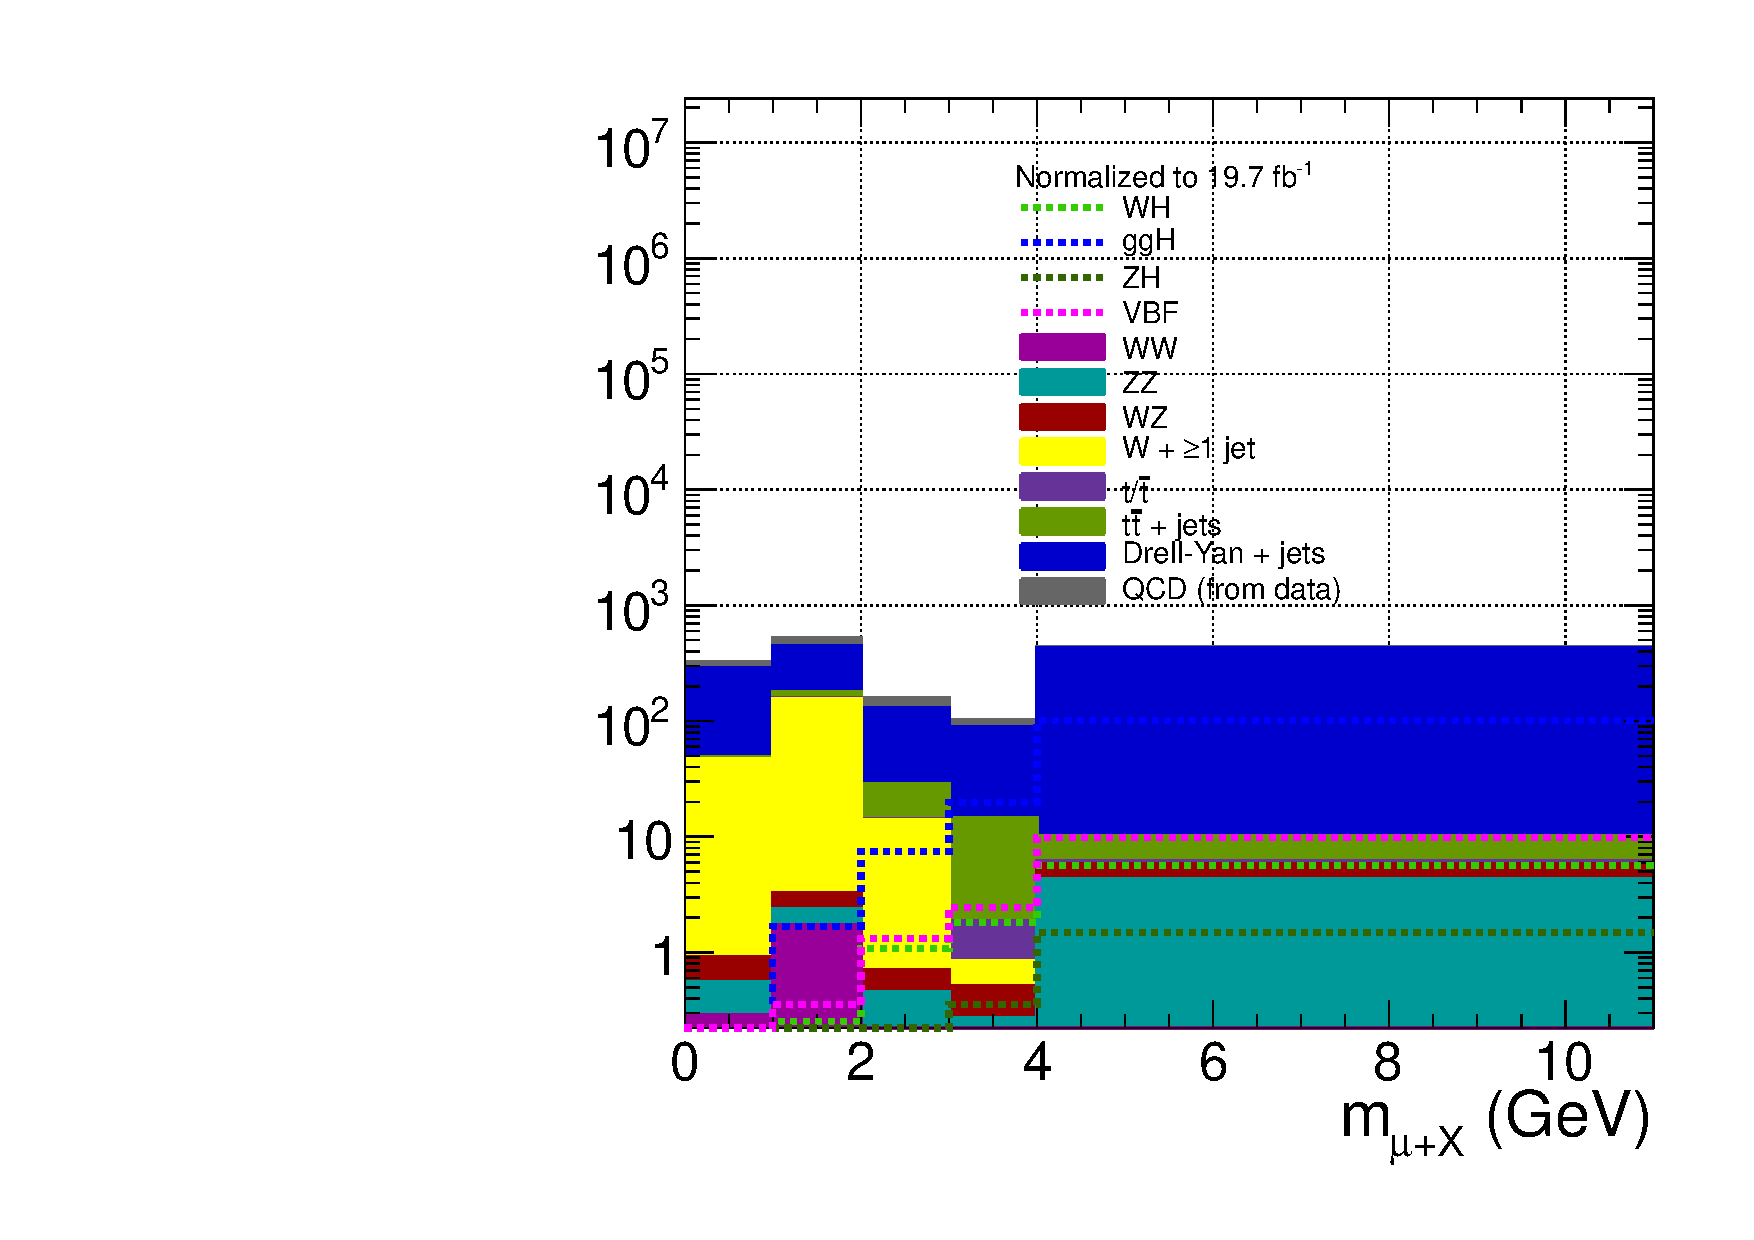
\includegraphics[width=1.2\cmsFigWidth]{figures/muHadMass_lowMT_beforeOSSF}
    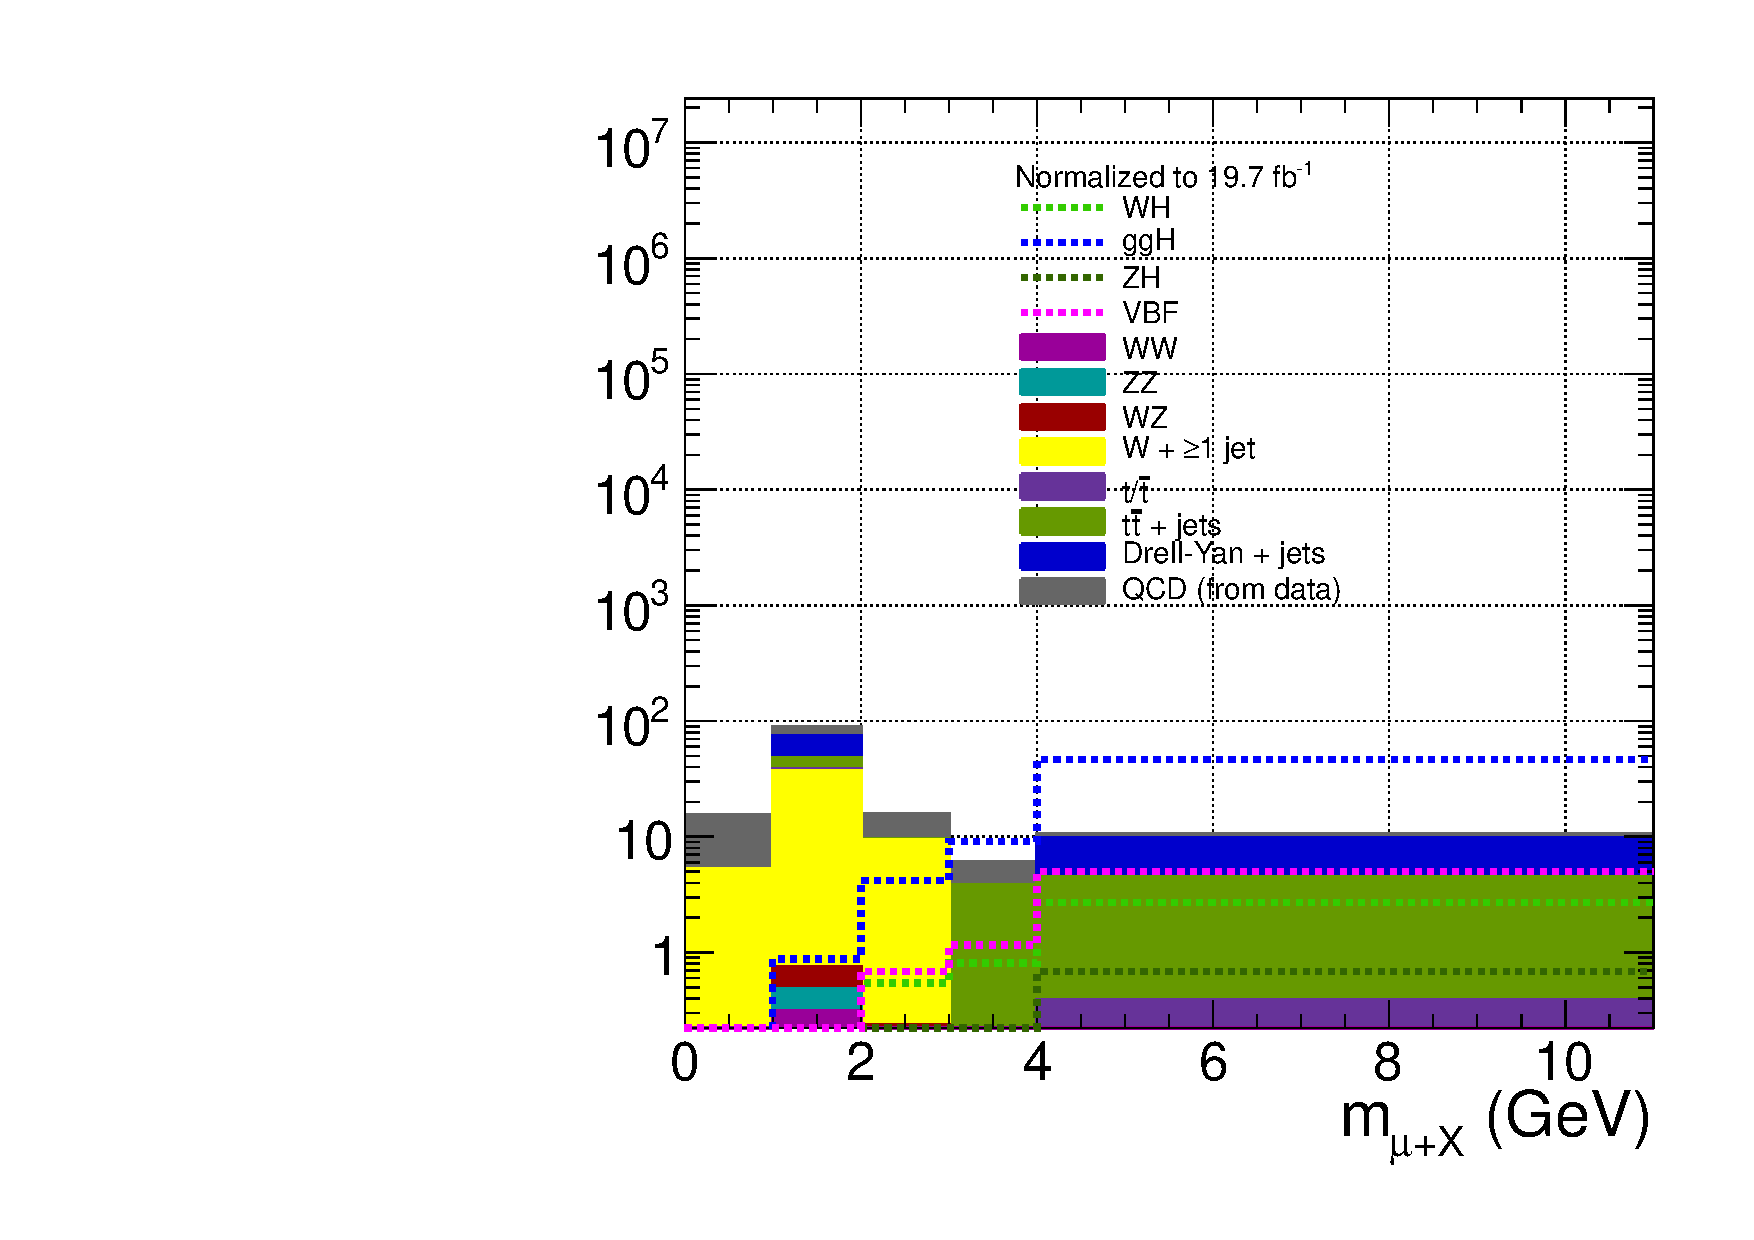
\includegraphics[width=1.2\cmsFigWidth]{figures/muHadMass_lowMT_afterOSSF}
    \caption{Invariant mass of the $\tau_{\mu}\tau_{\text{had}}$ pair for signals in the low-$M_{T}$ bin with $m_a$ = 9 GeV and all backgrounds before (\cmsLeft) and after (\cmsRight) the (trigger $\mu$)-$\tau_{\mu}$ same charge requirement.  All backgrounds except QCD are estimated from MC simulation. }
    \label{fig:muHadMass_OSSFVeto_vs_none_lowMT}
  \end{center}
\end{figure}

\begin{figure}[hbtp]
  \begin{center}
    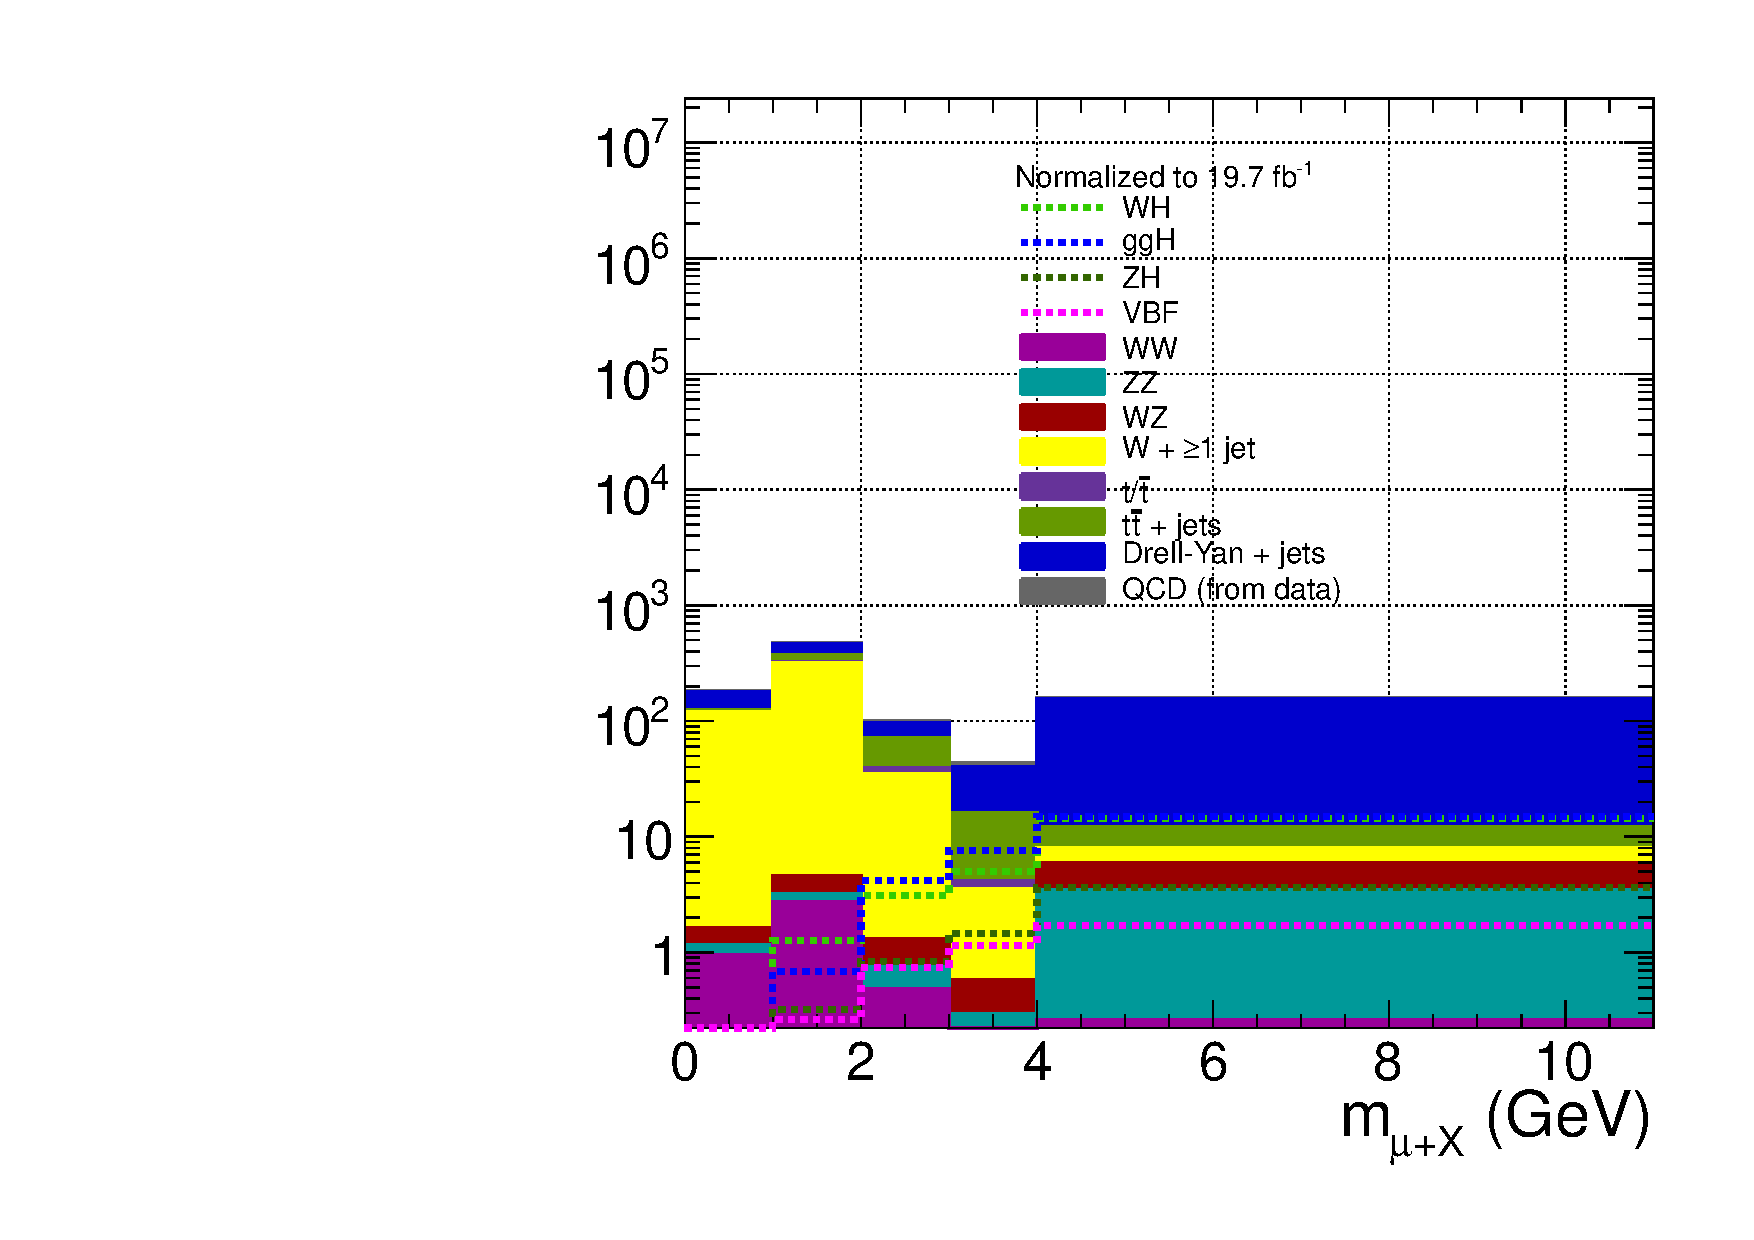
\includegraphics[width=1.2\cmsFigWidth]{figures/muHadMass_highMT_beforeOSSF}
    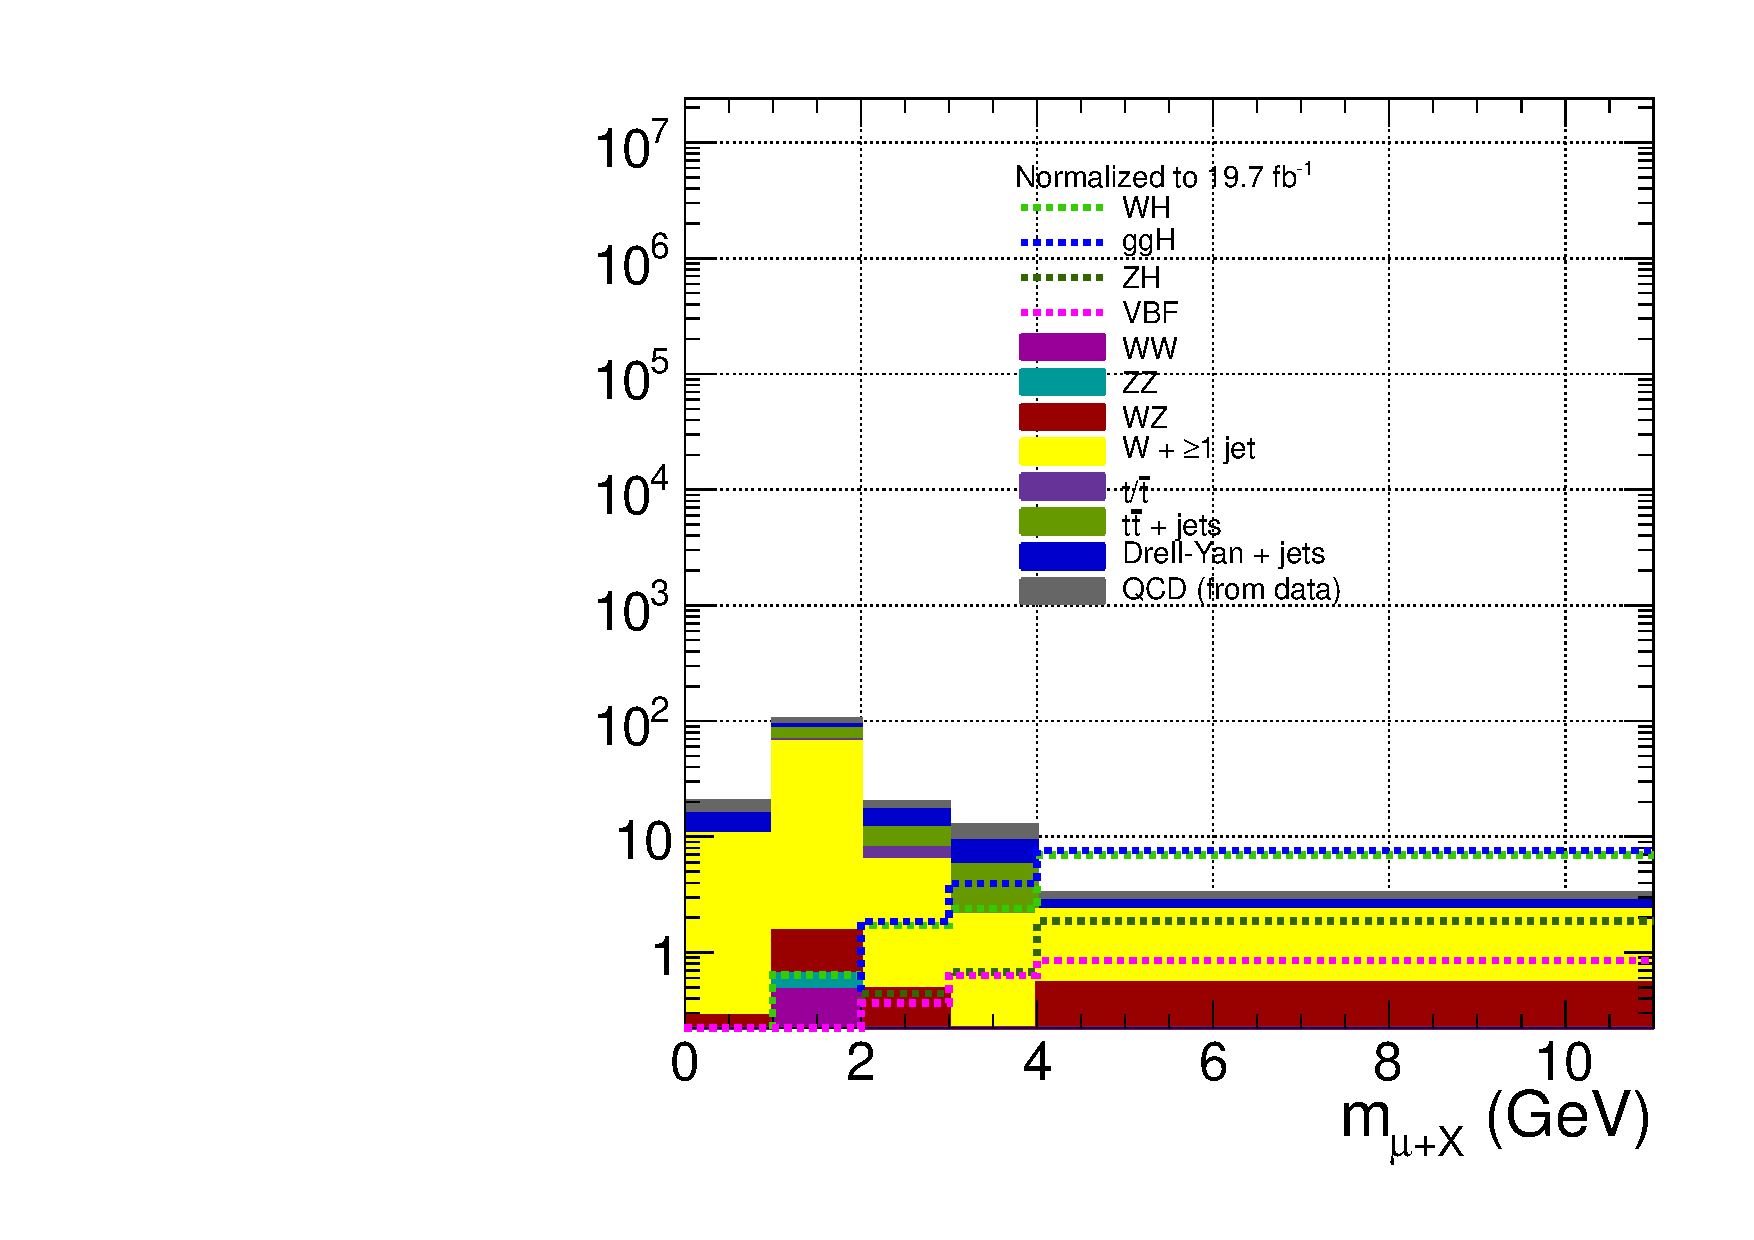
\includegraphics[width=1.2\cmsFigWidth]{figures/muHadMass_highMT_afterOSSF}
    \caption{Invariant mass of the $\tau_{\mu}\tau_{\text{had}}$ pair in the high-$M_{T}$ bin for signals with $m_a$ = 9 GeV and all backgrounds before (\cmsLeft) and after (\cmsRight) the (trigger $\mu$)-$\tau_{\mu}$ same charge requirement.  All backgrounds except QCD are estimated from MC simulation. }
    \label{fig:muHadMass_OSSFVeto_vs_none_highMT}
  \end{center}
\end{figure}

\section{Same charge tau veto\label{sec:evtsel-SSSF}}

$\tau_{\mu}\tau_{\text{had}}$ pairs are reconstructed in background events when there is a poorly isolated real muon, either promptly produced or coming from a heavy flavor jet, or when one track in a light jet fakes a soft muon and the others fake an HPS tau.  Fake $\tau_{\mu}\tau_{\text{had}}$ pairs rarely come from a real boosted di-tau decay, and therefore no correlation between the $\tau_{\mu}$ and $\tau_{\text{had}}$ charge is expected.  We therefore impose an opposite charge requirement on the $\tau_{\mu}$ and $\tau_{\text{had}}$, which reduces the background by about 20\% while leaving the signal virtually unchanged (Figure~\ref{fig:muHadMass_SSSF}).

\begin{figure}[hbtp]
  \begin{center}
    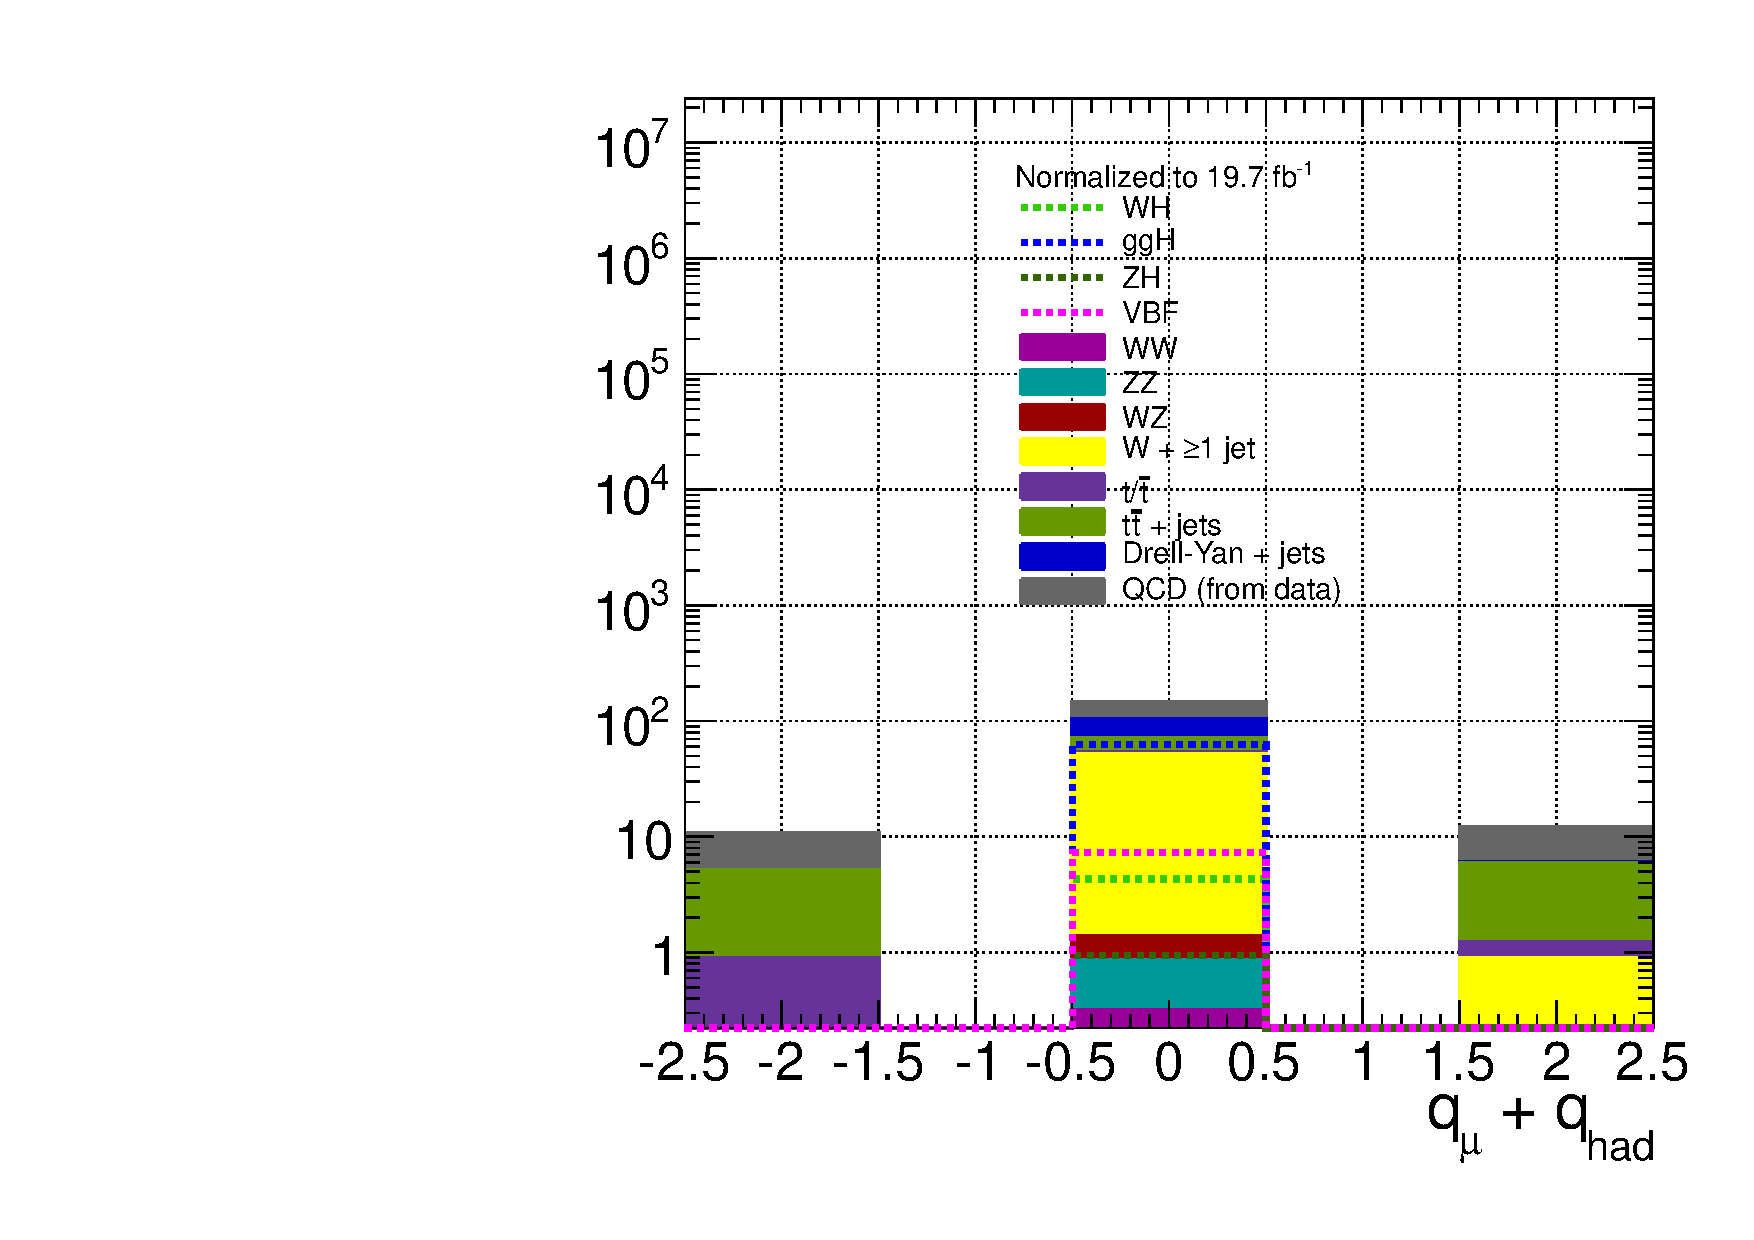
\includegraphics[width=1.2\cmsFigWidth]{figures/muHadCharge_lowMT_beforeSSSF}
    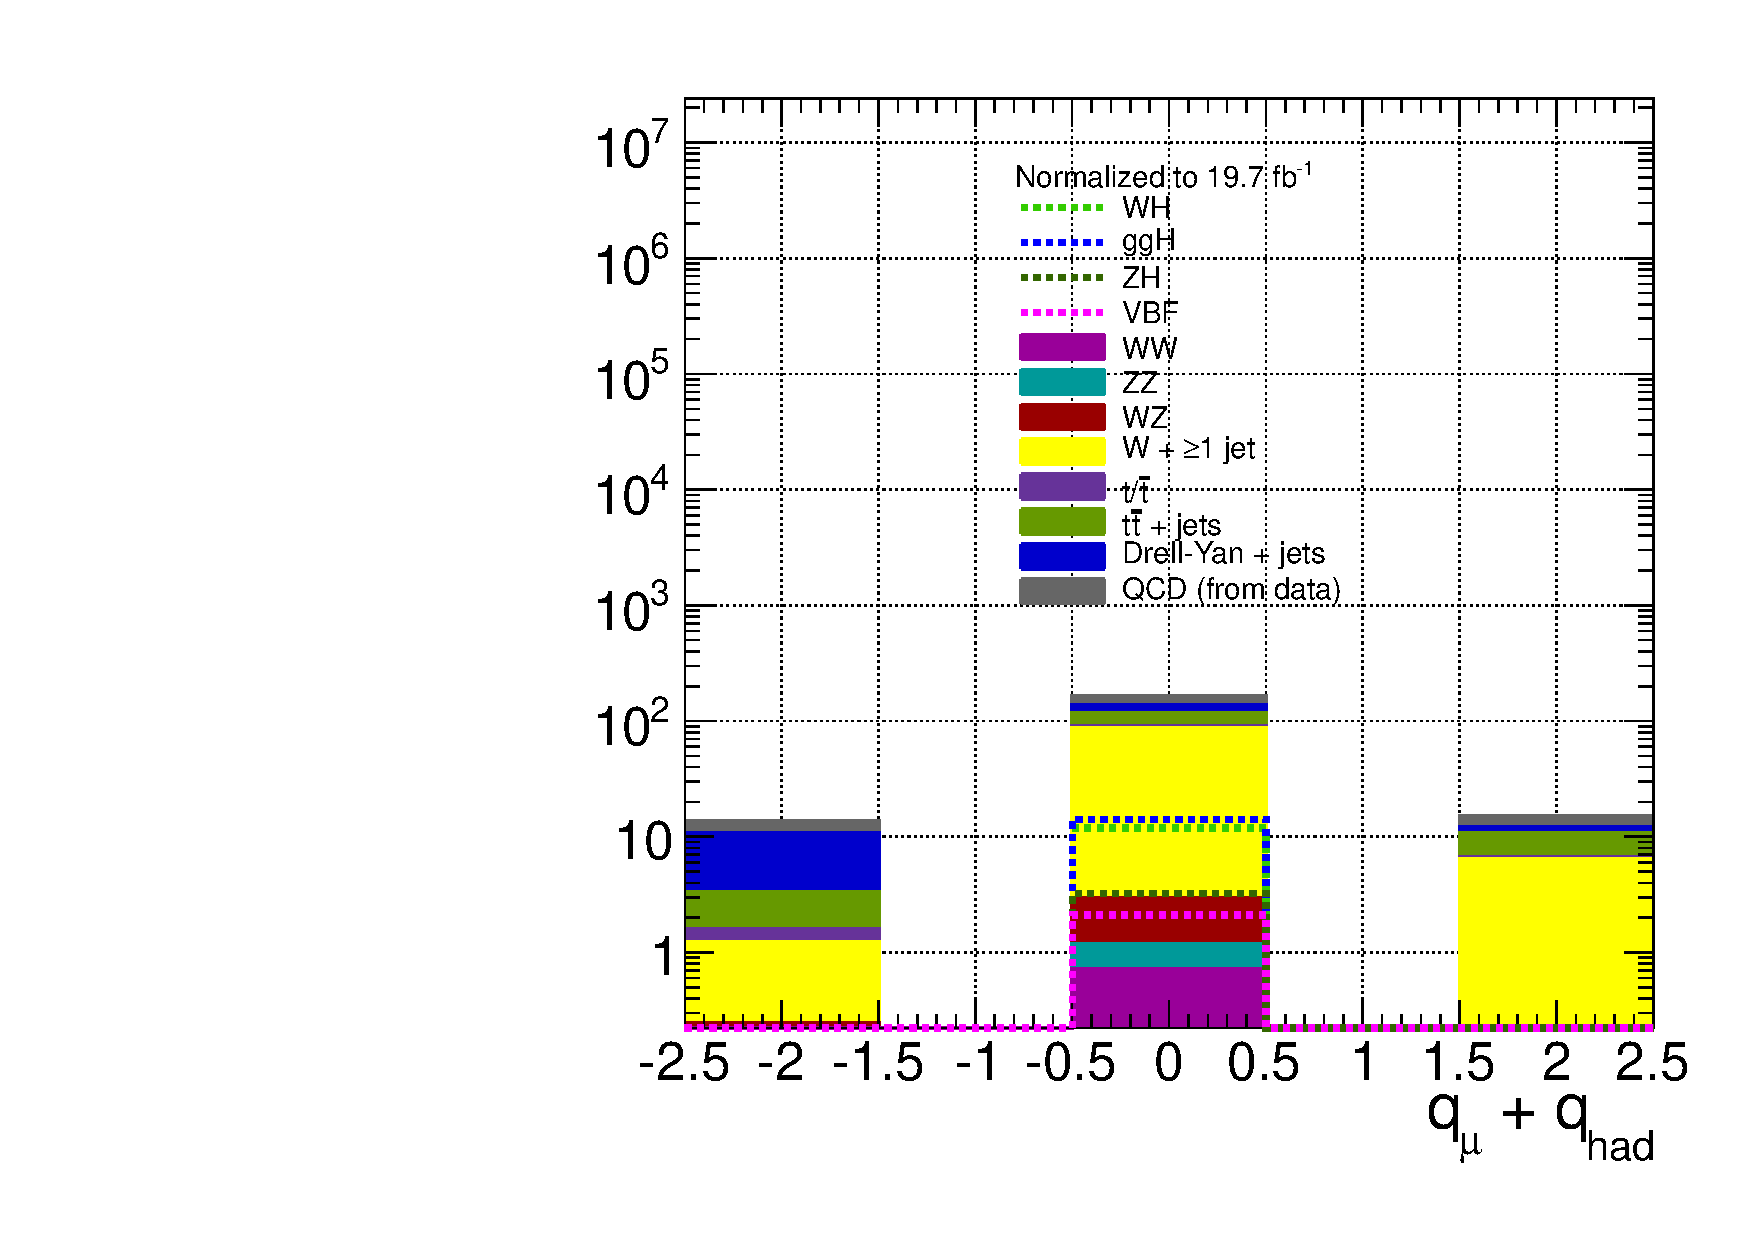
\includegraphics[width=1.2\cmsFigWidth]{figures/muHadCharge_highMT_beforeSSSF}
    \caption{Sum of the $\tau_{\mu}$ charge and $\tau_{\text{had}}$ charge for signals with $m_a$ = 9 GeV and all backgrounds.  All backgrounds except QCD are estimated from MC simulation. (\cmsLeft) Low-$M_{T}$ bin. (\cmsRight) High-$M_{T}$ bin. }
    \label{fig:muHadMass_SSSF}
  \end{center}
\end{figure}

%b-veto
\section{B-veto on tau jet\label{sec:evtsel-bveto}}

Heavy flavour jets, such as those from B meson or top decays, often contain a muon among the decay products which gets reconstructed as the $\tau_{\mu}$. Thus, the identification of b-jets can serve as a means to reject background from heavy flavour jets.

To optimize the identification of b-jets, b-tagging algorithms take advantage of the unique properties that distinguish b-jets from other kinds of jets produced at the LHC. One important property is the long lifetime of B mesons; when they decay, they will have travelled a significant distance (on the order of millimeters) from the primary vertex, resulting in displaced secondary vertices.  Thus, the impact parameter and secondary vertex associated with such jets can be used as discriminating variables. The combined secondary vertex (CSV) algorithm~\cite{Weiser:927399}, which is used in this search, employs a likelihood ratio that takes as input information about the primary vertex, secondary vertex, 2D and 3D impact parameters, track multiplicity, and track pseudorapidities of jets.

Figure~\ref{fig:sigVsBkg_csv_regA} shows the distribution of the CSV discriminator for Monte Carlo signals and all backgrounds except QCD in the low-$M_{\text{T}}$ and high-$M_{\text{T}}$ bins. As can be seen from this figure, the $\tau_{\text{had}}$ jet in the signal final states generally does not have large values of CSV; by vetoing b-tagged jets, the single top and $t\bar{t}$ backgrounds can be cut down significantly. A b-tag veto was thus implemented by rejecting events in which the cleaned jet associated with the $\tau_{\text{had}}$ object had a CSV value greater than the medium CSV working point of 0.679 recommended by the BTV POG for \texttt{22Jan2013} re-reco data at 8 \TeV~\cite{CMS:btvpogtwiki}.

\begin{figure}[hbtp]
  \begin{center}
    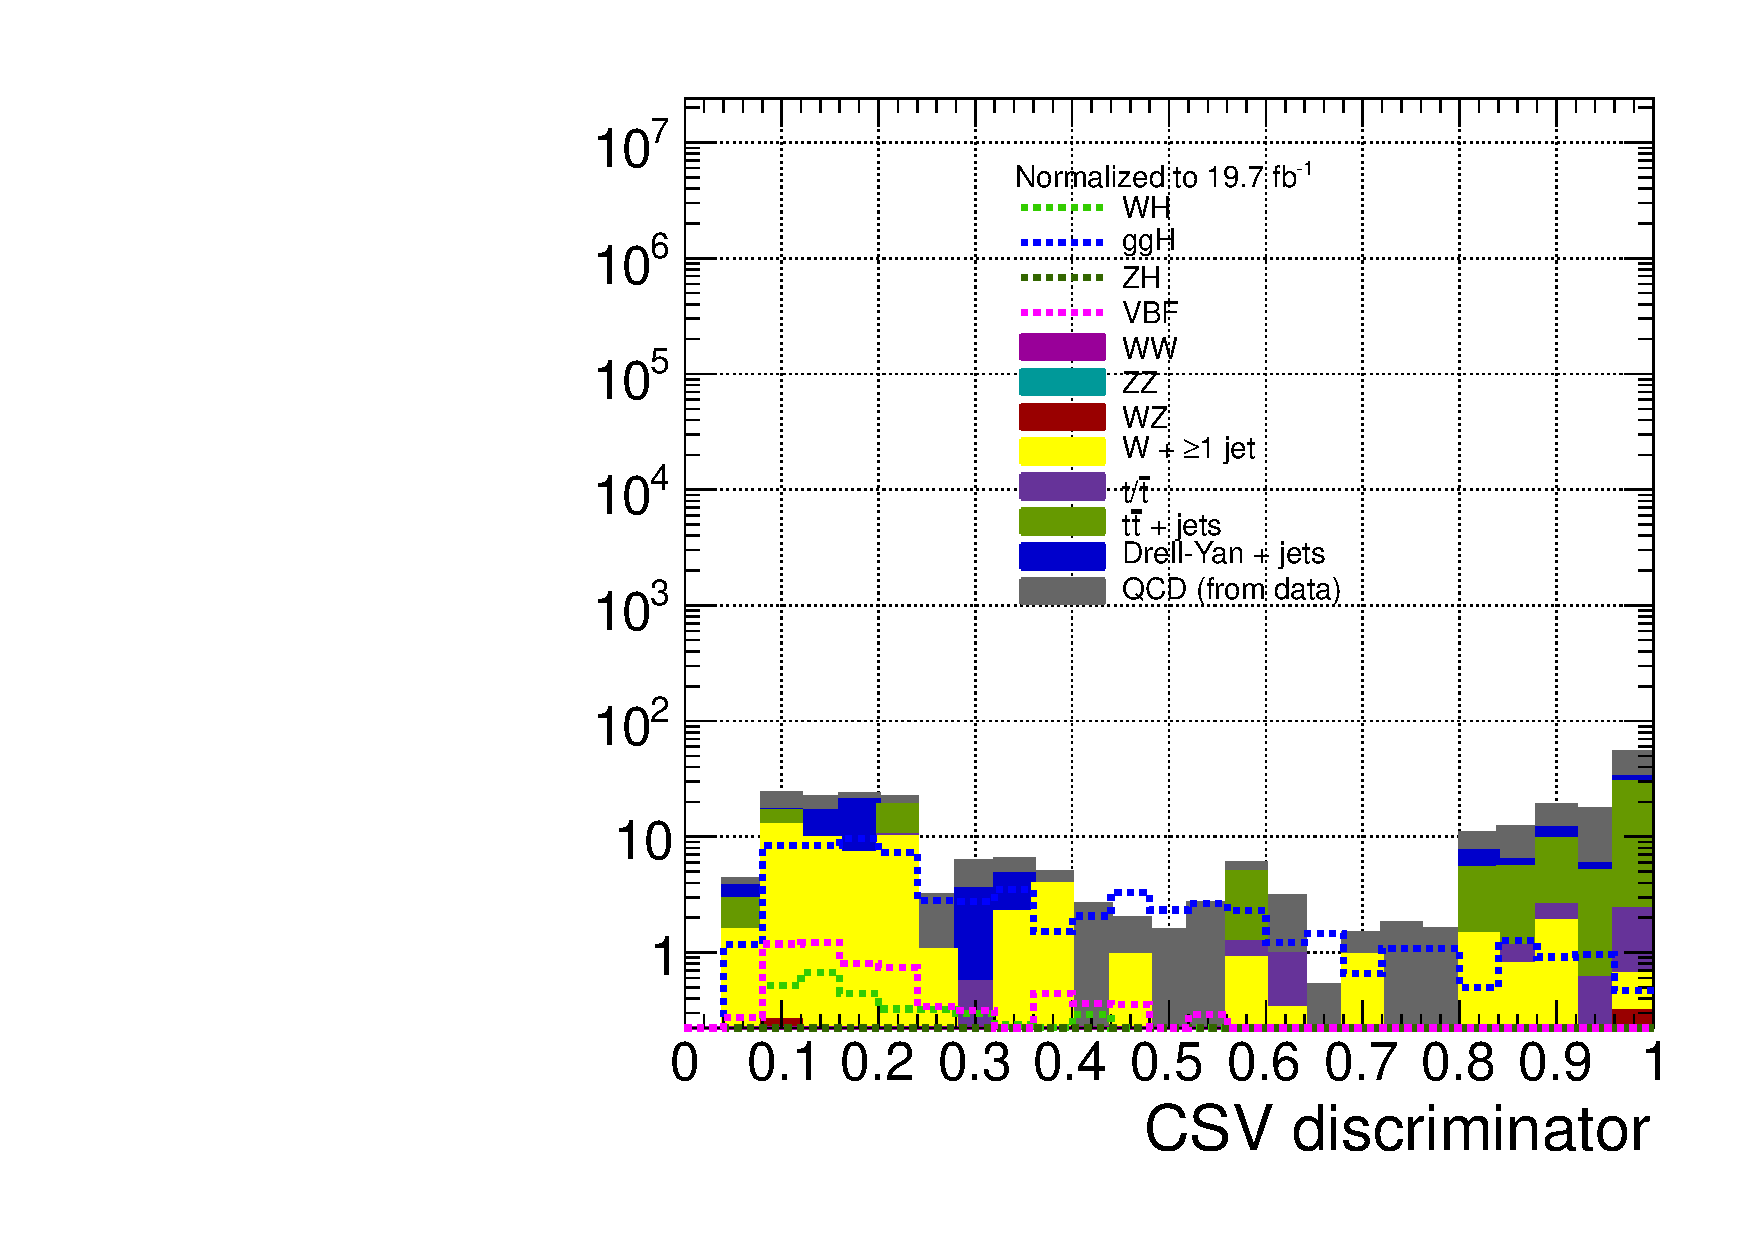
\includegraphics[width=\cmsFigWidth]{figures/sigVsBkg_csv_regA_lowMT_v61}
    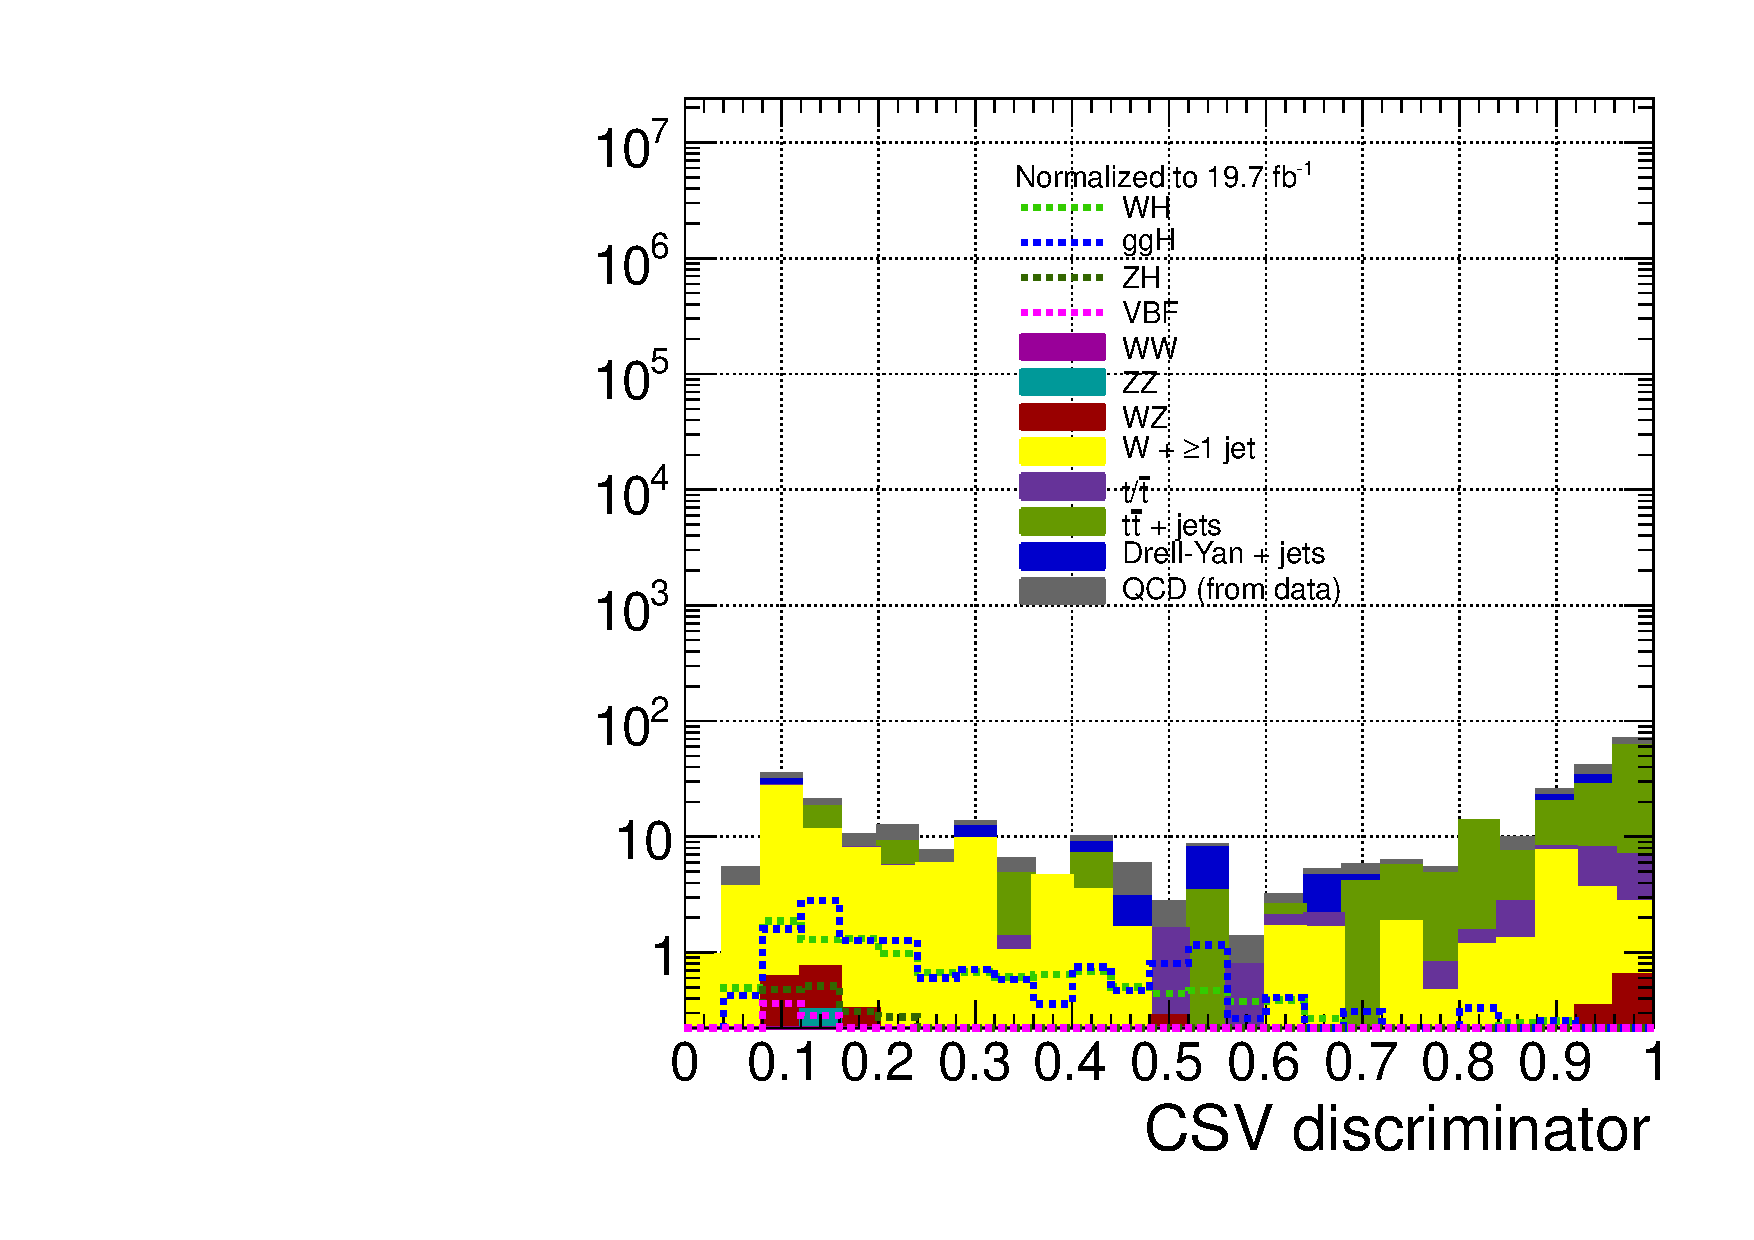
\includegraphics[width=\cmsFigWidth]{figures/sigVsBkg_csv_regA_highMT_v61}
    \caption{Distribution of the CSV discriminator for four signal models and all backgrounds, including data-driven QCD, after all the preselection cuts except the b veto have been applied. Normalized to 19.7 \fbinv. (\cmsLeft) Low-$M_{\text{T}}$ bin. (\cmsRight) High-$M_{\text{T}}$ bin.}
    \label{fig:sigVsBkg_csv_regA}
  \end{center}
\end{figure}

As shown in Figure~\ref{fig:sigVsBkg_csv_regA}, the distribution of the CSV discriminator for signal events tends to peak at low values of the discriminator, while single top and $t\bar{t}$ events with real b-jets peak at high values; thus, since no data/MC b-veto efficiency scale factors exist for tau jets, we make the approximation that the tau jets in our signal behave more like light jets with regard to the CSV discriminator, and so the expected signal is corrected for differences between data and MC b-veto efficiency using the BTV-provided scale factors~\cite{CMS:btaguncertaintytwiki} for light jets.  The scale factors are binned in HPS tau parent (cleaned) jet $\eta$ and $p_T$.

\begin{figure}[hbtp]
  \begin{center}
    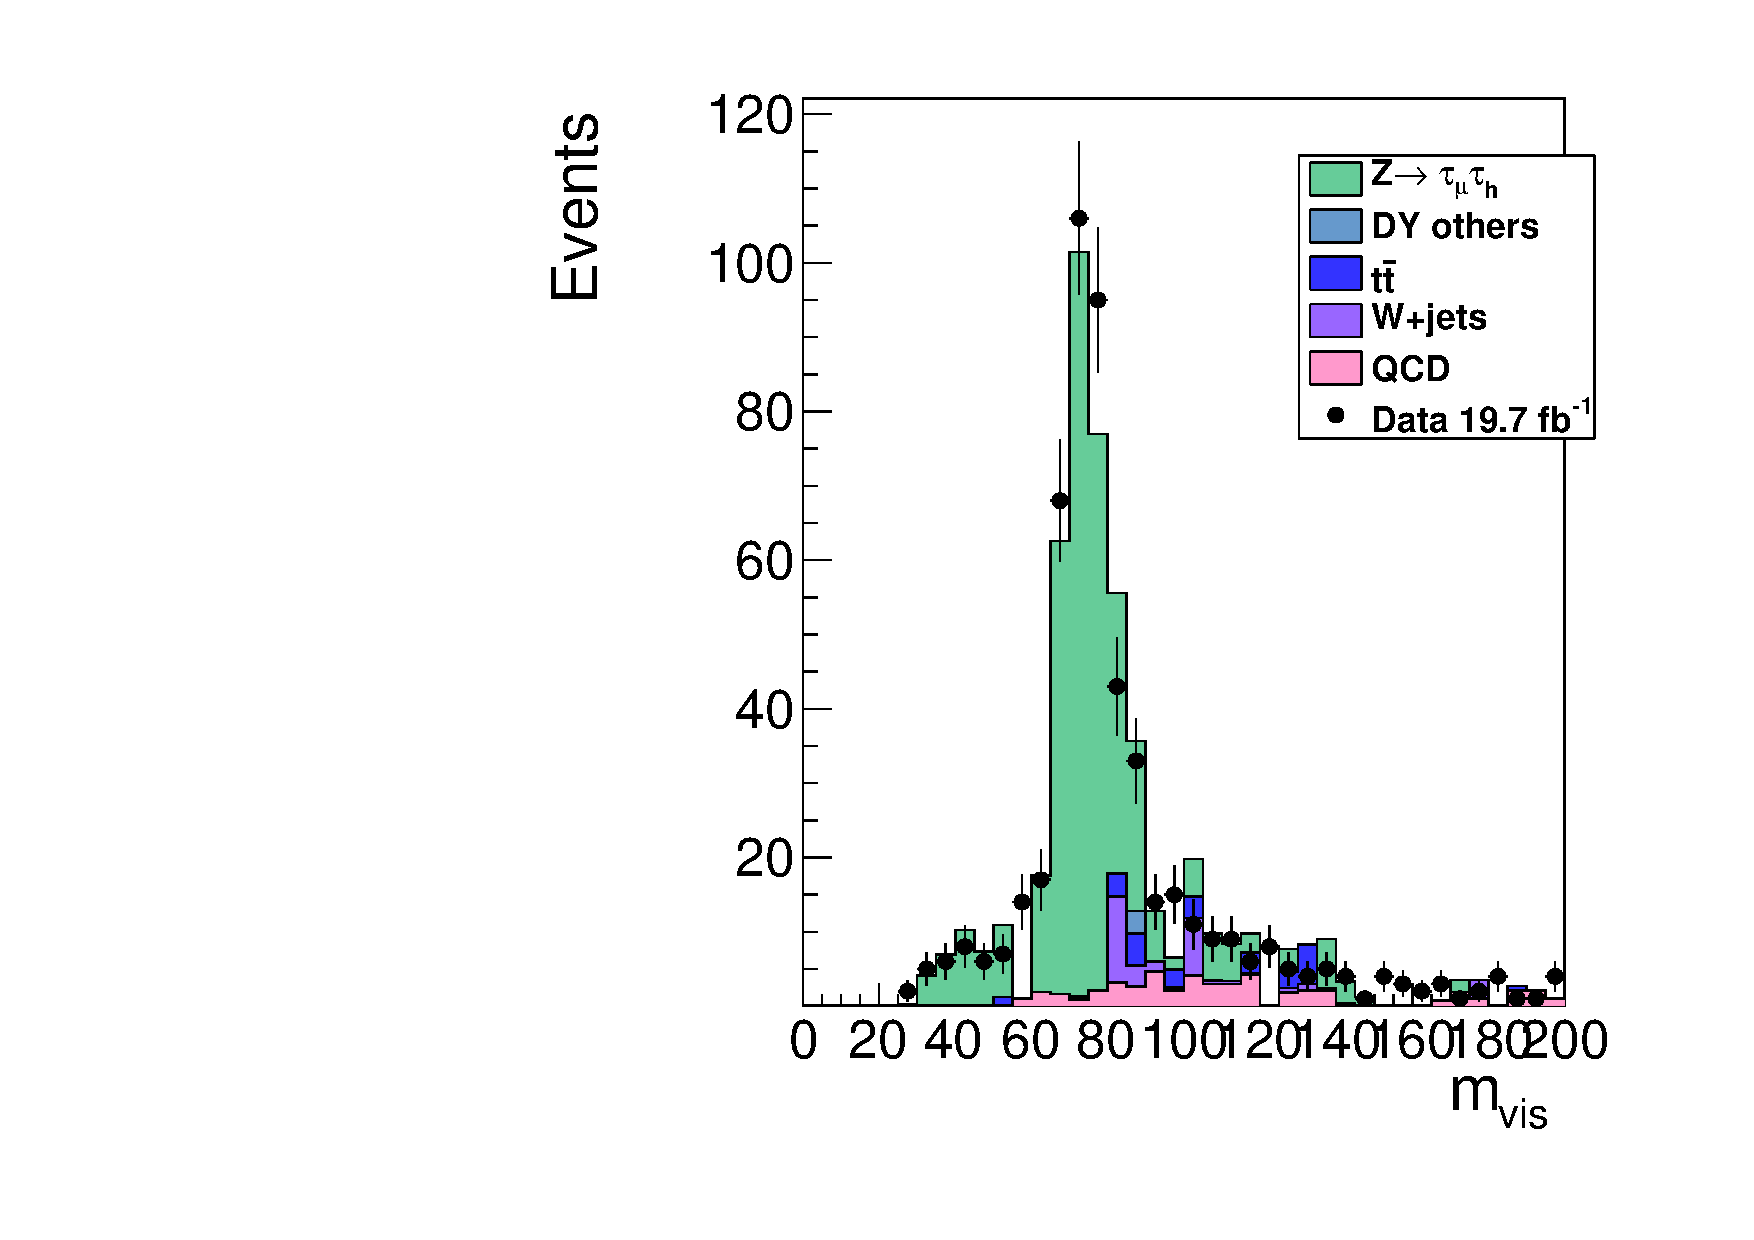
\includegraphics[width=\cmsFigWidth]{figures/PassNN_mvis}
    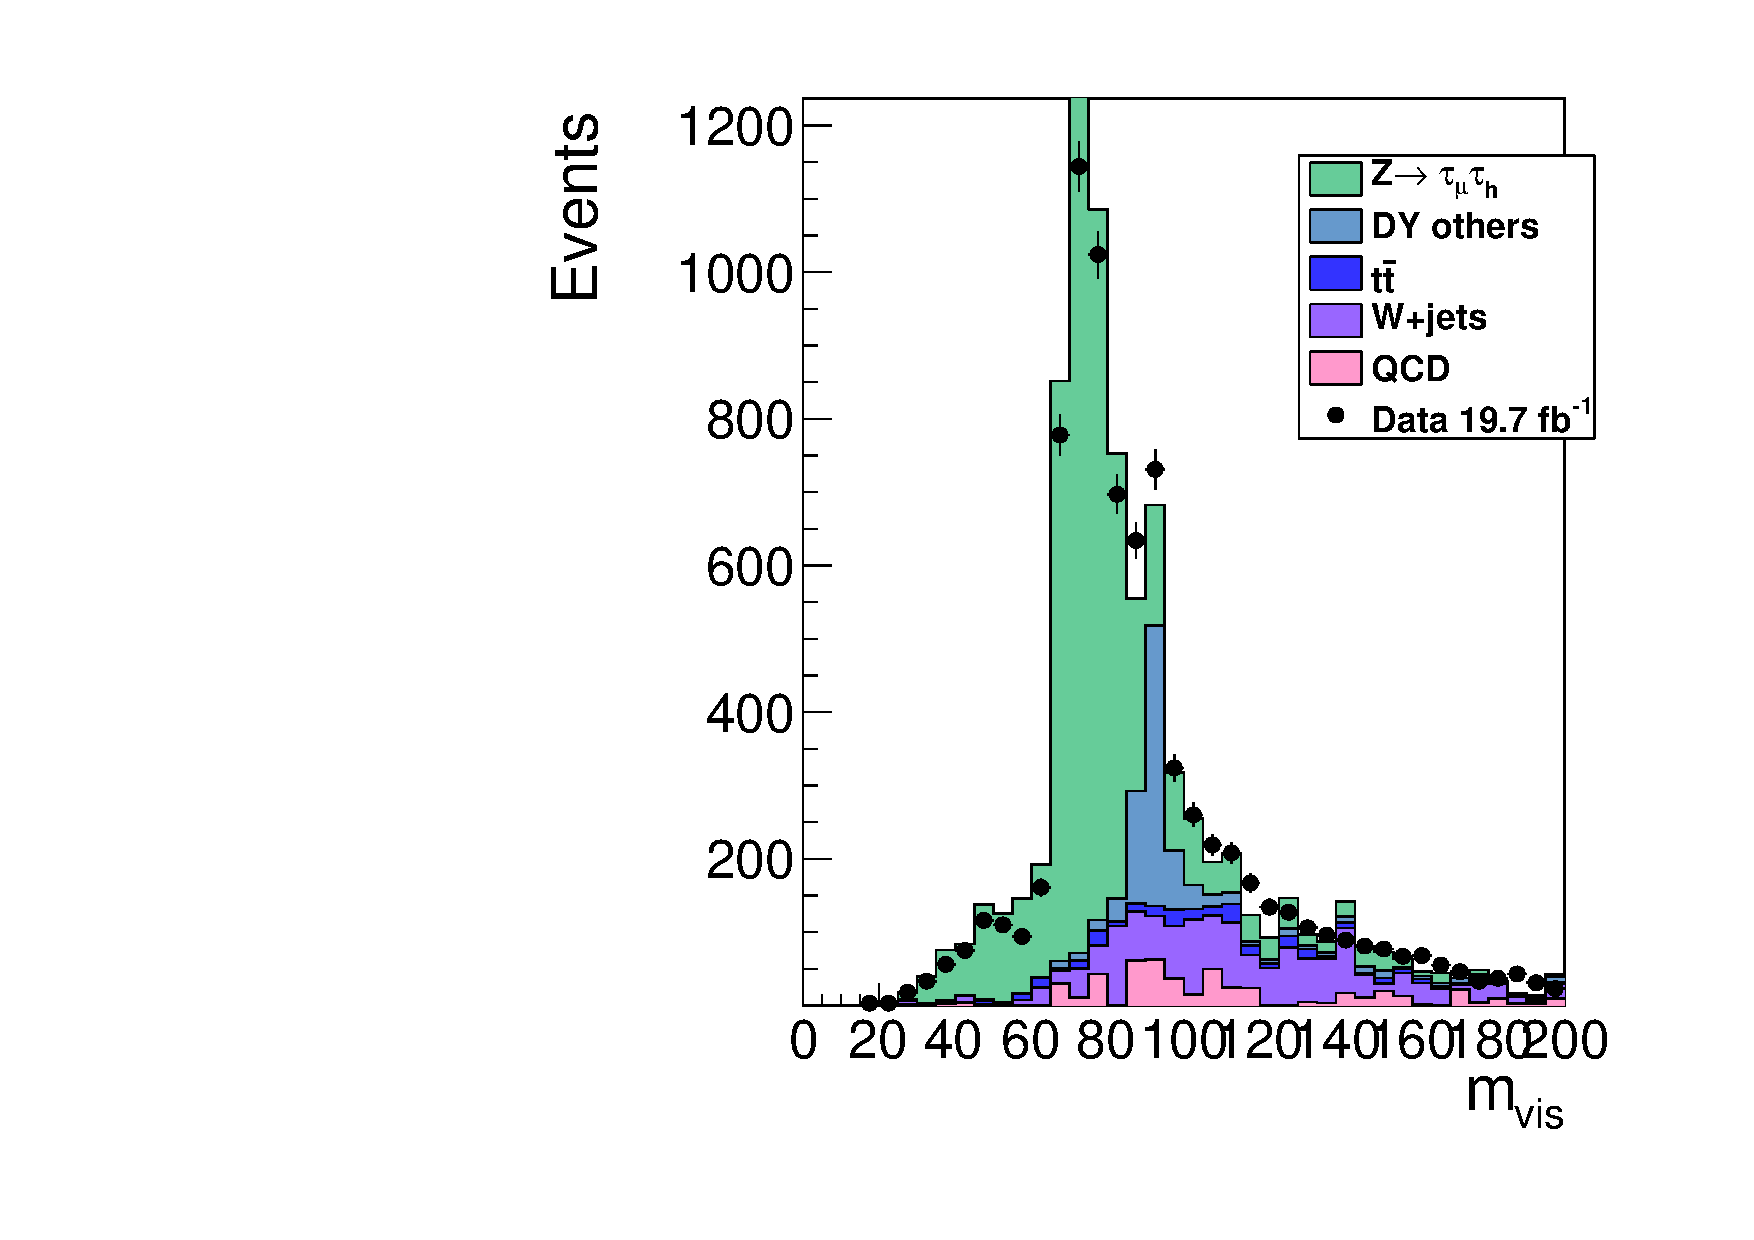
\includegraphics[width=\cmsFigWidth]{figures/FailNN_mvis}
    \caption{$\tau_{\mu}\tau_{\text{had}}$ invariant mass plots showing Z peak in Run I data and MC, for events passing all Z peak selections including the medium combined isolation discriminator for $\tau_{\text{had}}$, and passing or failing the medium CSV b-tag applied to the jet that seeded the $\tau_{\text{had}}$. (\cmsLeft) Events passing the medium CSV b-tag. (\cmsRight) Events failing the medium CSV b-tag.}
    \label{fig:BTagZPeakPassFail}
  \end{center}
\end{figure}

Two methods are used to assess the error on the expected signal due to the uncertainty on the scale factors. Firstly, the expected signal is recalculated for a coherent +1$\sigma$ shift in the scale factors in all simulated events, and then again for a -1$\sigma$ shift; the difference between the nominal and $\pm1\sigma$-shifted expected signal is taken as the $\pm1\sigma$ error due to b-tag scale factors for light jets. Secondly, another systematic is calculated to account for the uncertainty of using light-jet scale factors for tau jets; the signal yields after the final selection are calculated using light-jet scale factors (the nominal method) and using b-jet scale factors (the logic being that the phase space for tau jets should be somewhere between the two extremes of light jets and b jets), and the percent difference in the yield is taken as a conservative uncertainty on the yield due to the usage of light-jet scale factors.

Since a b-veto is applied to a tau jet, the following cross-check has been performed to verify that the assigned systematic uncertainty for a potential data/MC discrepancy is adequate. First, a clean sample of of tau lepton candidates was obtained using $Z\rightarrow\tau_{\mu}\tau_{\text{had}}$ selections in Run I data and MC and the Z peak was reconstructed as per the methods in~\cite{Tau14001}, requiring that the $\tau_{\text{had}}$ object pass the medium combined isolation discriminator. Then, additionally, a b-tag at the medium CSV working point was applied to the jets that seeded the $\tau_{\text{had}}$, and two Z peaks were plotted -- one for events passing the b-tag and one for events failing the b-tag. The Z peak plots are shown in Figure~\ref{fig:BTagZPeakPassFail}; these results suggest that the data/MC agreement is unaffected by whether the tau jets pass or fail the CSV b-tag, and also it can be seen that the percentage of events in data and MC that pass the medium CSV b-tag is in the neighbourhood of 10\%, which is similar to the proportion of signal MC events observed to pass the medium CSV b-tag. Thus, these results lend confidence to the assumption that the requirement for the tau jet to pass the medium CSV b-veto does not significantly affect the known data/MC discrepancy covered by the present systematic uncertainty.

%PV
\section{Primary vertex compatibility requirement\label{sec:evtsel-dz}}
To reduce the background from $\tau_{\mu}\tau_{\text{had}}$ pairs in which the $\tau_{\mu}$ and $\tau_{\text{had}}$ come from different $pp$ interactions, we require $d_{\text{z}}(\tau_{\mu},\text{PV}) <$ 0.5 \cm and $d_{\text{z}}(\tau_{\text{had}},\text{PV}) <$ 0.2 cm, where PV refers to the hardest (primary) interaction in the event.  These cuts are recommended by the MUO and TAU POGs.  The $d_{\text{z}}(\tau_{\mu},\text{PV})$ and $d_{\text{z}}(\tau_{\text{had}},\text{PV})$ distributions for events passing all preselection cuts except those plotted are shown in Figures~\ref{fig:sigVsBkg_dz_regA_lowMT} and~\ref{fig:sigVsBkg_dz_regA_highMT}.

\begin{figure}[hbtp]
  \begin{center}
    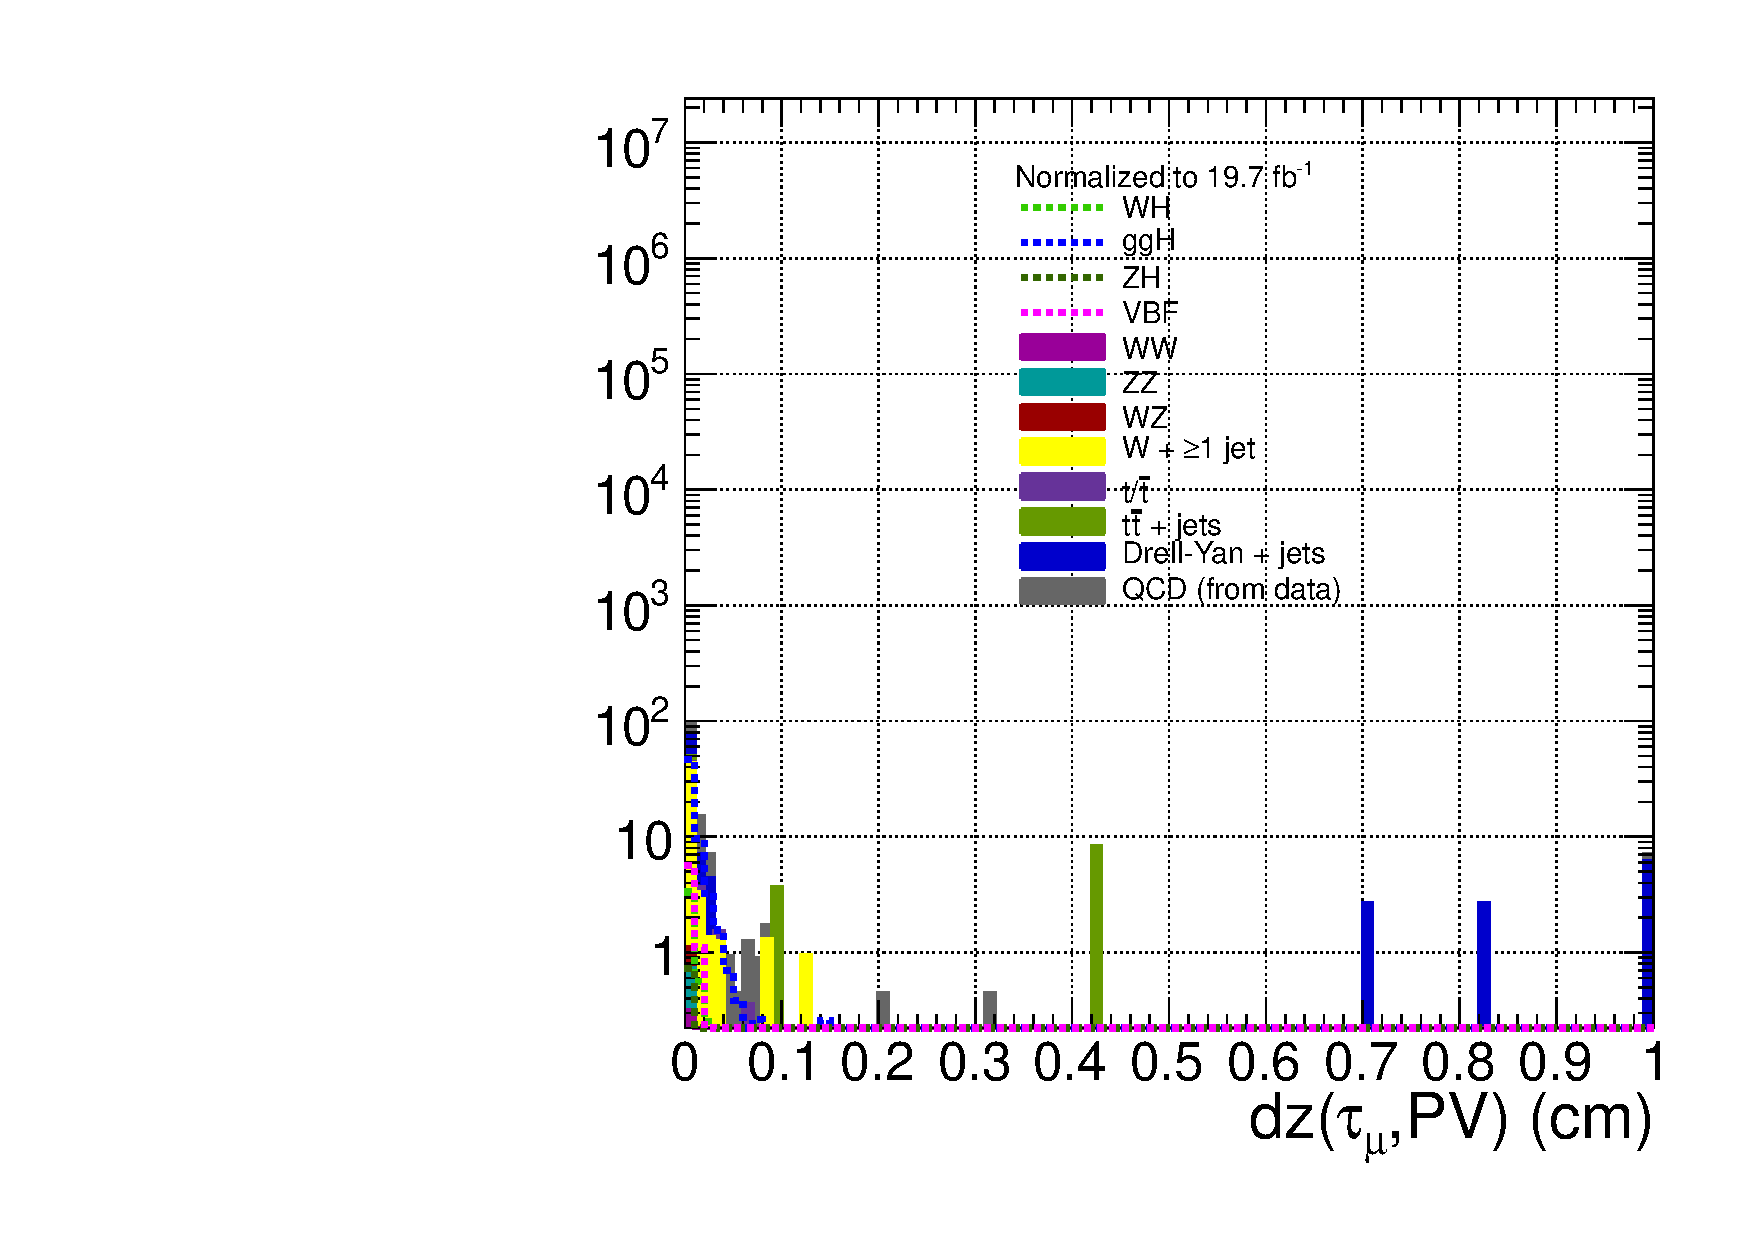
\includegraphics[width=1.2\cmsFigWidth]{figures/sigVsBkg_dztaumu_regA_lowMT_v60}
    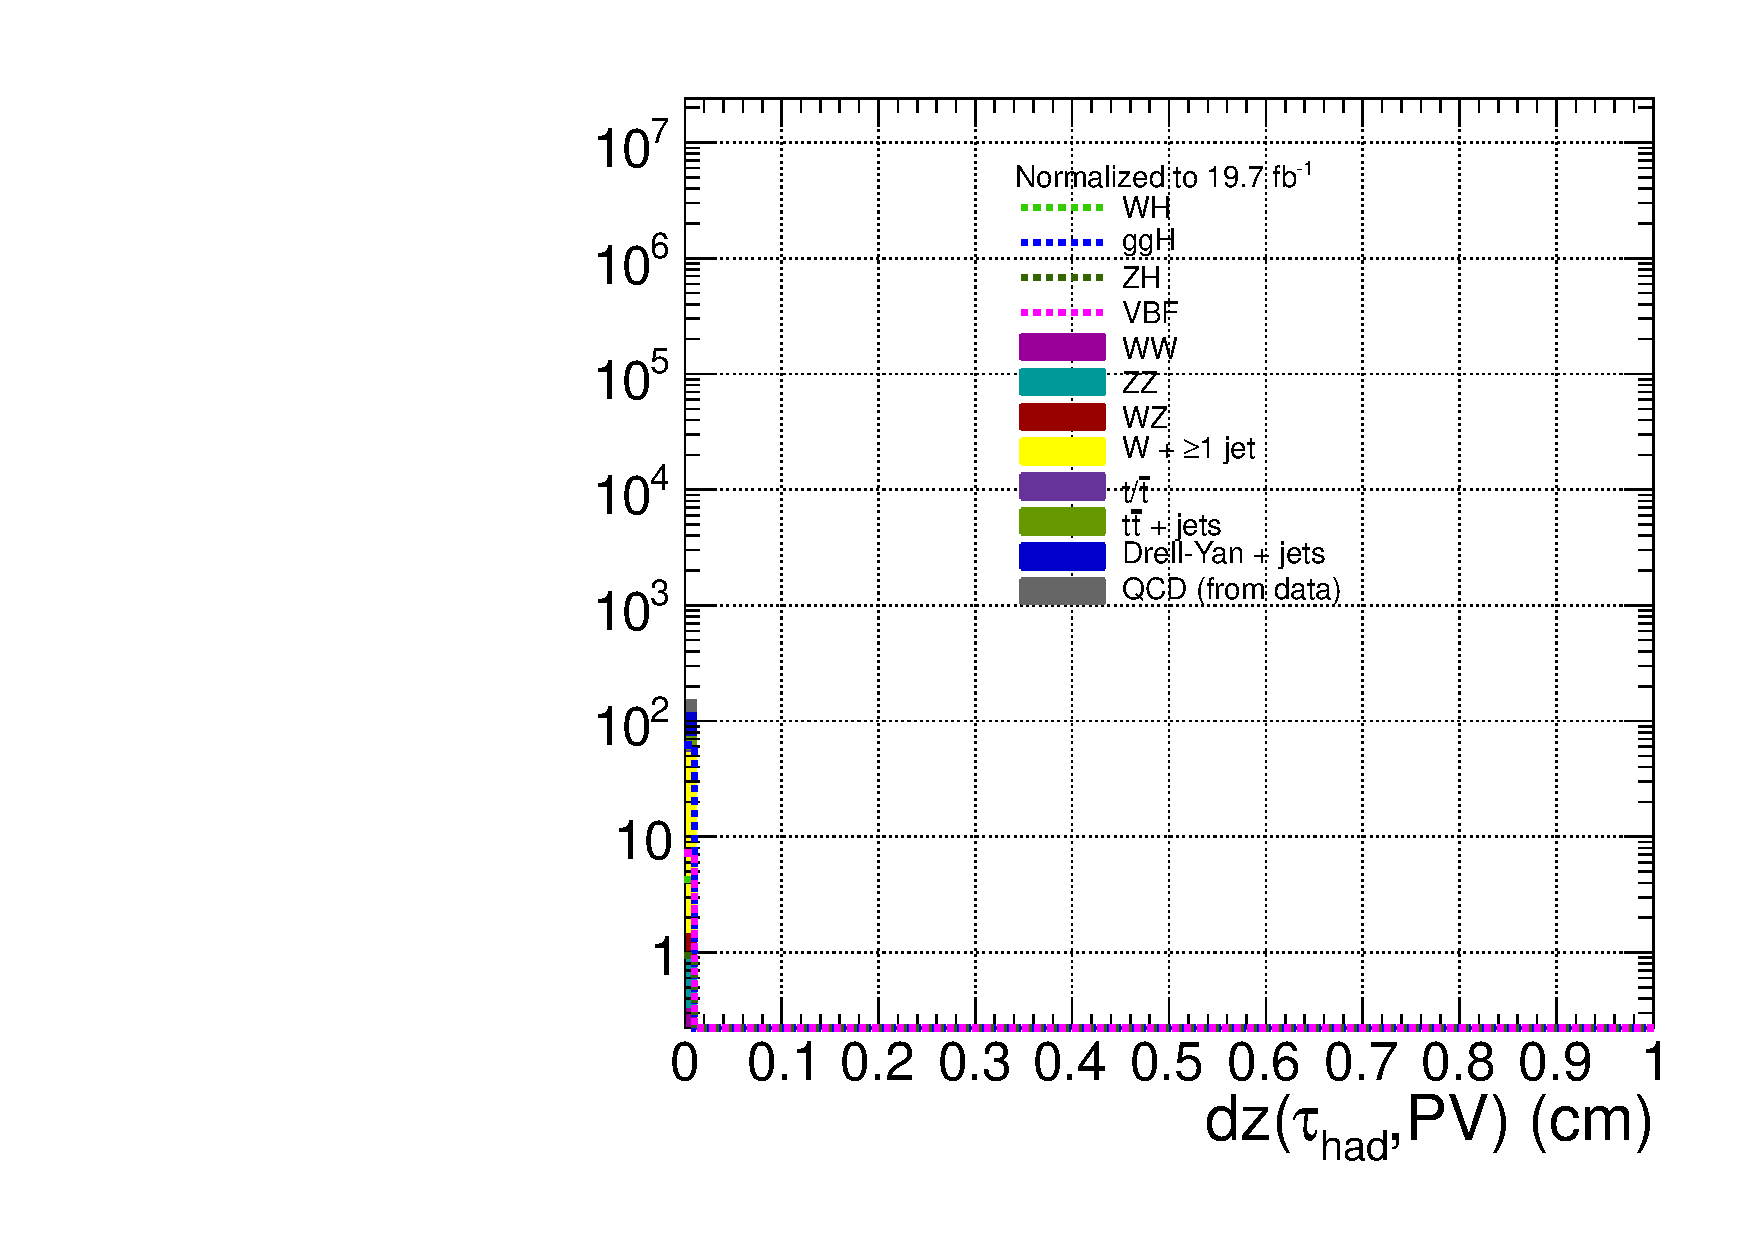
\includegraphics[width=1.2\cmsFigWidth]{figures/sigVsBkg_dztauhad_regA_lowMT_v60}
    \caption{Distribution of (\cmsLeft) dz($\tau_{\mu}$,PV) and (\cmsRight) dz($\tau_{\text{had}}$,PV) in the low-$M_{T}$ bin for four signal models and all backgrounds including data-driven QCD, after all the preselection cuts except the dz cuts have been applied. Normalized to 19.7 \fbinv.}
    \label{fig:sigVsBkg_dz_regA_lowMT}
  \end{center}
\end{figure}

\begin{figure}[hbtp]
  \begin{center}
    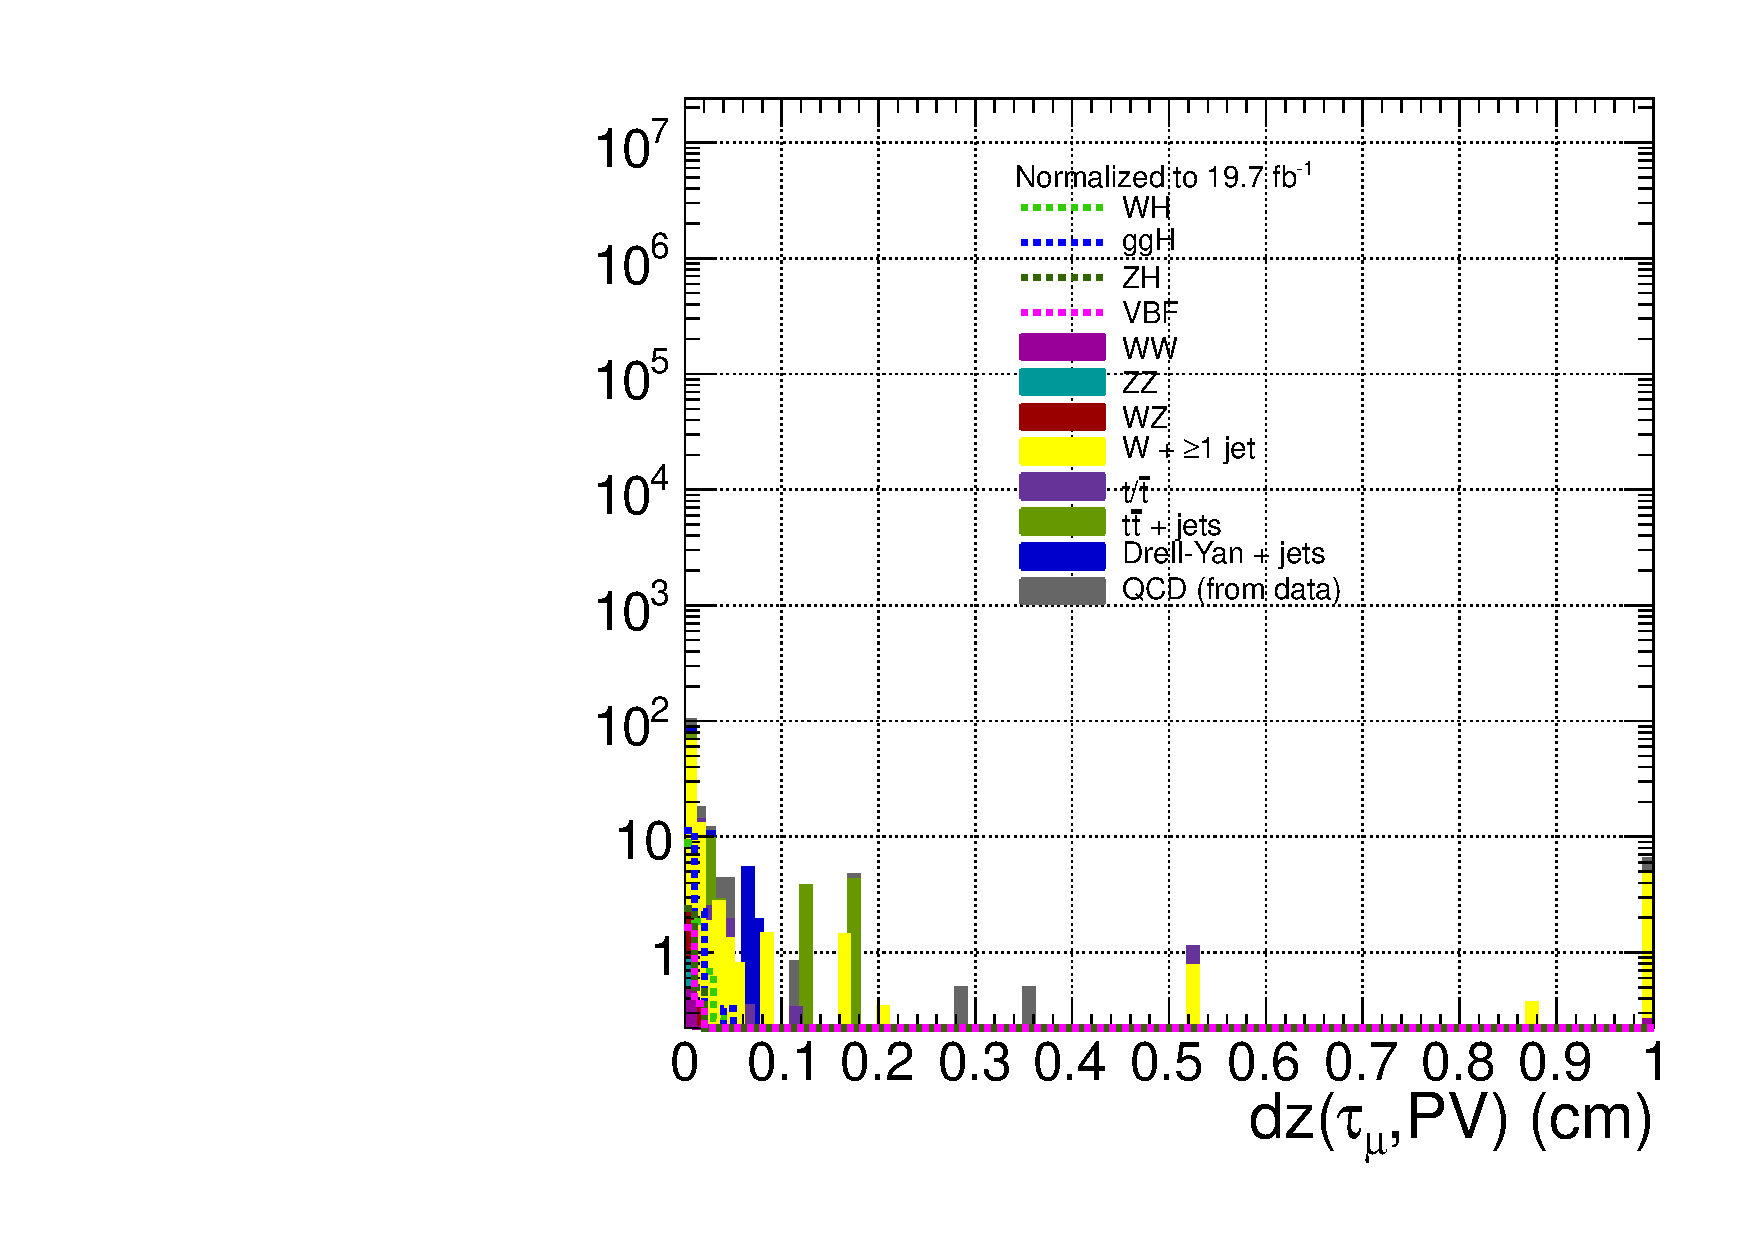
\includegraphics[width=1.2\cmsFigWidth]{figures/sigVsBkg_dztaumu_regA_highMT_v60}
    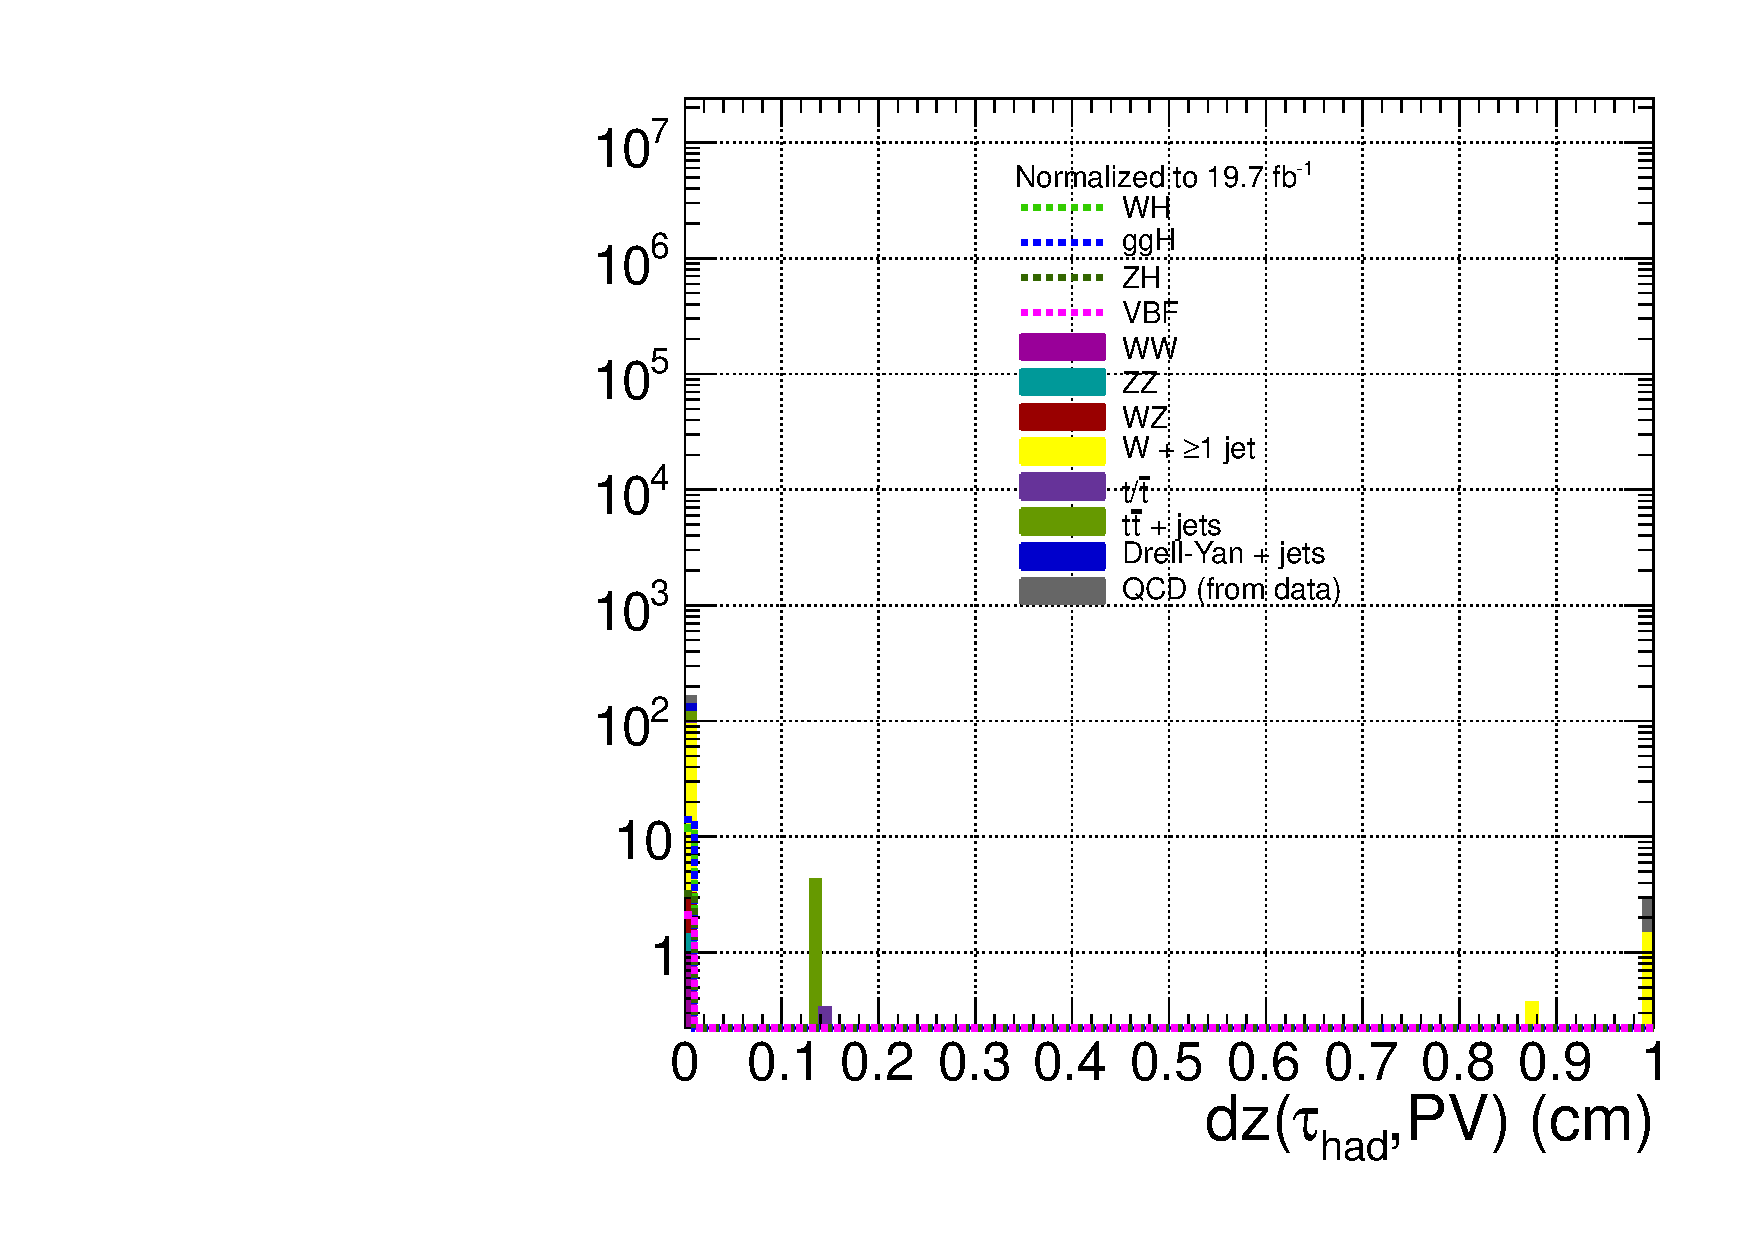
\includegraphics[width=1.2\cmsFigWidth]{figures/sigVsBkg_dztauhad_regA_highMT_v60}
    \caption{Distribution of (\cmsLeft) dz($\tau_{\mu}$,PV) and (\cmsRight) dz($\tau_{\text{had}}$,PV) in the high-$M_{T}$ bin for four signal models and all backgrounds including data-driven QCD, after all the preselection cuts except the dz cuts have been applied. Normalized to 19.7 \fbinv.}
    \label{fig:sigVsBkg_dz_regA_highMT}
  \end{center}
\end{figure}

%MT
\section{Transverse mass regions \label{sec:evtsel-mt}}

Figure~\ref{fig:sigVsBkg_MET_MT_regA} shows the $M_{\text{T}}$ distribution for four signal models and all backgrounds.  The gluon fusion signal is clustered at low $M_{\text{T}}$, where Drell-Yan and QCD are the most important backgrounds.  The WH signal can be found in the high $M_{\text{T}}$ bin, where $W$+jets and $t\bar{t}$ dominate the background.  We define $M_{\text{T}} \le$ 50 GeV as the low-$M_{\text{T}}$ bin of this search, sensitive to ggH and VBF, and $M_{\text{T}} >$ 50 GeV as the high-$M_{\text{T}}$ bin, sensitive to WH.  The cut was chosen to optimize S/$\sqrt{\text{S} + \text{B}}$ for the WH signal in the high-$M_{\text{T}}$ bin.  The $M_{\text{T}}$ in this search is calculated using Type I-corrected~\cite{1748-0221-6-11-P11002} PAT \ETslash, which is also used in the calculation of \ETslash systematics~\cite{METuncertainty}.

\begin{figure}[hbtp]
  \begin{center}
    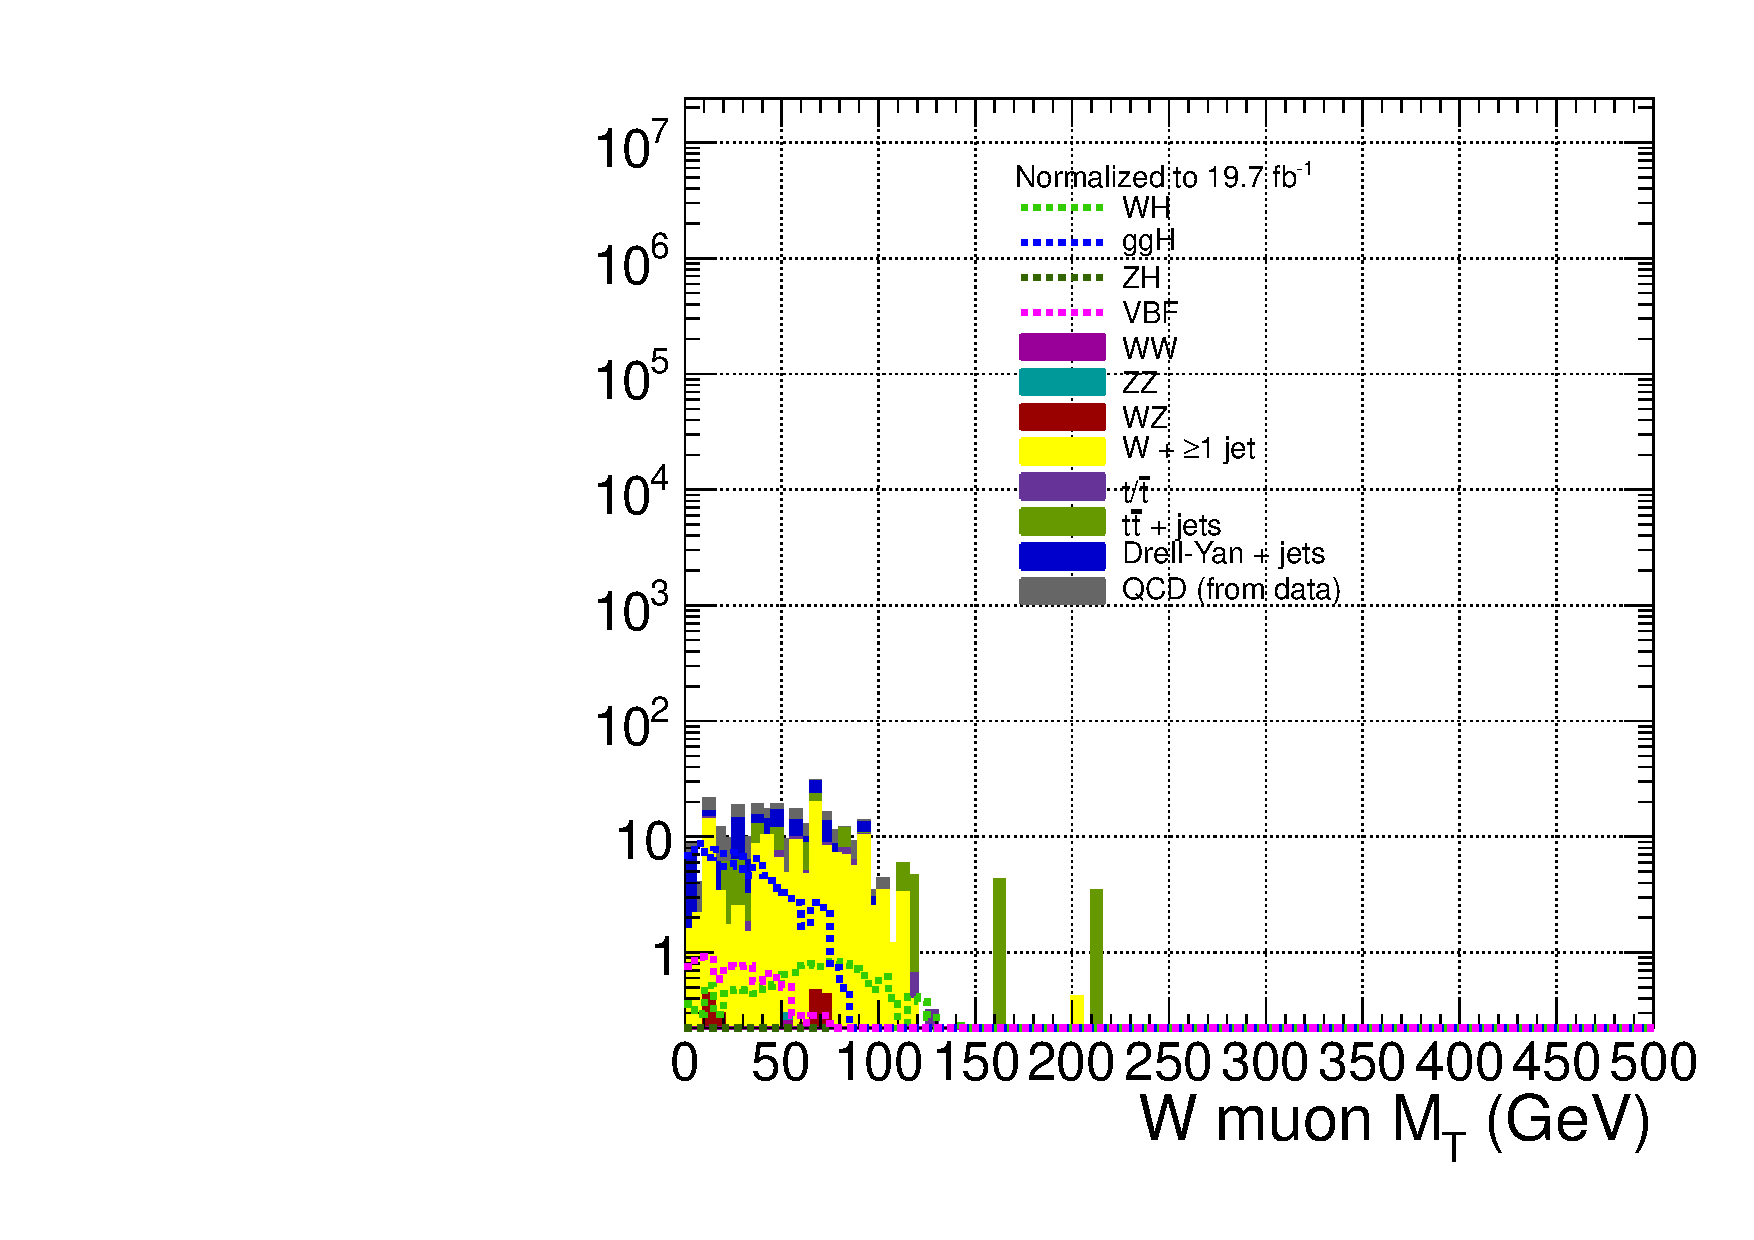
\includegraphics[width=1.2\cmsFigWidth]{figures/sigVsBkg_MT_regA_v62}
    \caption{$M_{\text{T}}$ distribution after the preselection (excluding the $M_{\text{T}}$ cut) has been applied for four signal models and all backgrounds. The term ``$W$ muon'' in the label refers to the trigger muon, not necessarily a muon from a $W$ decay (as in the case of the ggH signal, for instance).}
    \label{fig:sigVsBkg_MET_MT_regA}
  \end{center}
\end{figure}

Following the JME approved procedure~\cite{METuncertainty}, uncertainty on the expected signal in each $M_{\text{T}}$ bin due to \ETslash scale is assessed by independently varying the e/$\gamma$, muon, tau, jet, and unclustered energy scales up and down by their approved 1$\sigma$ errors for each event in the signal sample.  \ETslash and $M_{\text{T}}$ are recalculated in each event, yielding an expected signal estimate in each of the +1$\sigma$ and -1$\sigma$ scenarios.  For each energy scale variation, the larger of the $\pm1\sigma$ deviations from nominal is taken as the error due to the uncertainty on that energy scale.  The quadrature sum of these individual errors is taken as the total $\pm1\sigma$ error due to \ETslash scale.

For technical reasons, the \ETslash definition for the $\pm1\sigma$ varied \ETslash collections and the nominal from which deviations are measured is slightly different from the \ETslash definition used when quoting the expected signal.  However, the deviations for the \ETslash uncertainty calculation are measured in a consistent way (same \ETslash definition for varied and nominal collections), and it is only the percent difference which is quoted as the \ETslash scale error.

%Final selection
\section{Search region \label{sec:evtsel-search}}
Table~\ref{tab:cut-flow-MC} shows the number of events surviving each successive cut in the selection sequence for the $m_a$ = 9 GeV WH and ggH signal samples and all background Monte Carlo samples (except for QCD Monte Carlo, due to poor statistics) used in the selection sequence optimization.  Table~\ref{tab:cut-flow-WHSignal} displays the selection efficiencies for the WH signal samples for each selection cut, expressed as the fraction of triggered signal events (i.e., events passing the HLT) surviving after each cut.  Table~\ref{tab:cut-flow-ggHSignal} shows the analogous selection efficiencies for the ggH signal samples.  The number of events is scaled to 19.7 fb$^{-1}$ using the cross sections given in Tables~\ref{tab:MCBkg} and~\ref{tab:MC-sig}.

%\begin{table*}[htbh]
\begin{sidewaystable}
\begin{center}
\caption{Number of events in MC signal and background datasets remaining after each cut in the selection sequence.  The signal samples have a pseudoscalar mass of 9 GeV.  The number of events is scaled to 19.7 \fbinv using the cross sections given in Tables~\ref{tab:MCBkg} and~\ref{tab:MC-sig}.  For the rows labeled ``$d_{\text{Z}}$ to PV'' and ``$m_{\mu+\text{had}} >$ 4 GeV'', pileup reweighting has been applied, while for the other rows, no pileup reweighting has been applied.\label{tab:cut-flow-MC}}
\resizebox{\columnwidth}{!}{
\begin{tabular}{|m{2.5cm}|c|c|c|c|c|c|c|c|c|c|c|}
  \hline
  \multicolumn{2}{|l|}{Cut} & WH & ggH & W+$\ge$1 jet & Drell-Yan + jets & $t\bar{t}$ + jets & Single top & WZ & ZZ & WW \\
  \hline
  \hline
  \multicolumn{2}{|l|}{} & 4.522\ten{3} & 6.721\ten{4} & 1.883\ten{8} & 3.587\ten{8} & 4.842\ten{6} & 1.825\ten{6} & 6.542\ten{5} & 3.478\ten{5} & 1.080\ten{6} \\
  \hline
  \multicolumn{2}{|l|}{\texttt{HLT\_IsoMu24\_eta2p1}} & 1.024\ten{3} & 6.616\ten{3} & 2.723\ten{7} & 1.507\ten{7} & 6.359\ten{5} & 1.124\ten{5} & 5.203\ten{4} & 1.937\ten{4} & 1.167\ten{5} \\
  \hline
  \multicolumn{2}{|l|}{Trigger $\mu p_T$} & 1.001\ten{3} & 6.083\ten{3} & 2.633\ten{7} & 1.459\ten{7} & 6.238\ten{5} & 1.091\ten{5} & 5.090\ten{4} & 1.913\ten{4} & 1.138\ten{5} \\
  \hline
  \multicolumn{2}{|l|}{Trigger $\mu \eta$, ID, and isolation} & 9.065\ten{2} & 4.417\ten{3} & 2.410\ten{7} & 1.381\ten{7} & 5.543\ten{5} & 9.936\ten{4} & 4.732\ten{4} & 1.816\ten{4} & 1.043\ten{5} \\
  \hline
  \multicolumn{2}{|l|}{$\tau_{\mu} p_T$, $\eta$, and ID} & 2.702\ten{2} & 2.600\ten{3} & 2.950\ten{5} & 3.705\ten{6} & 1.449\ten{5} & 1.430\ten{4} & 7.300\ten{3} & 6.842\ten{3} & 6.138\ten{3} \\
  \hline
  \multicolumn{2}{|l|}{HPS $\eta$ and ID} & 1.270\ten{2} & 9.838\ten{2} & 7.518\ten{4} & 9.074\ten{4} & 6.805\ten{4} & 6.508\ten{3} & 7.541\ten{2} & 6.257\ten{2} & 7.861\ten{2} \\
  \hline
  \multicolumn{2}{|l|}{HPS $p_T$ and isolation}                          & 39.06 & 216.0 & 1145  & 4338   & 798.3 & 85.56  & 24.53  & 24.35  & 13.18 \\
  \hline
  \multicolumn{2}{|l|}{b-veto}                              & 34.28 & 194.8 & 903.6 & 4170   & 273.2 & 20.40  & 20.41  & 21.93  & 10.26 \\
  \hline
  \multicolumn{2}{|l|}{HLT matching}                                   & 33.99 & 194.0 & 903.6 & 4088   & 266.1 & 20.40  & 19.95  & 21.33  & 10.05 \\
  \hline
  \multicolumn{2}{|l|}{$q(\tau_{\mu}) \times q(\text{trigger }\mu)$} & 16.70 & 92.56 & 171.0 & 93.21  & 81.60 & 8.365  & 3.075  & 1.455  & 1.404 \\
  \hline
  \multicolumn{2}{|l|}{$q(\tau_{\mu}) \times q(\tau_{\text{had}})$}     & 16.55 & 91.80 & 154.3 & 68.84  & 67.41 & 6.901  & 2.159  & 1.171  & 1.296 \\
  \hline
  \multicolumn{2}{|l|}{Trigger $\mu$ nearby lepton filter}       & 16.37 & 79.80 & 153.1 & 68.84  & 63.86 & 6.901  & 2.159  & 1.171  & 1.296 \\
  \hline
  \hline
  \multicolumn{2}{|l|}{\textbf{$M_{\text{T}} >$ 50 GeV}}              & 12.04 & 14.91 & 95.40 & 22.66  & 39.03 & 5.389  & 1.701  & 0.4968 & 0.8642 \\
  \hline
  \multicolumn{2}{|r|}{$d_{\text{Z}}$ to PV}                           & 11.77 & 13.52 & 84.15 & 20.85  & 25.10 & 4.306  & 1.783  & 0.4766 & 0.7122 \\
  \hline
  \multicolumn{2}{|r|}{$m_{\mu+\text{had}} >$ 4 GeV} & 6.972 & 7.598 & 1.761 & 0.4630 & 0     & 0      & 0.4038 & 0.1447 & 0 \\
  \hline
  \hline
  \multicolumn{2}{|l|}{\textbf{$M_{\text{T}} \le$ 50 GeV}}            & 4.326 & 64.89 & 57.67 & 46.18  & 24.84 & 1.512  & 0.4580 & 0.6743 & 0.4321 \\
  \hline
  \multicolumn{2}{|r|}{$d_{\text{Z}}$ to PV}                           & 4.225 & 60.79 & 50.30 & 32.03  & 17.62 & 1.839  & 0.5187 & 0.5394 & 0.3159 \\
  \hline
  \multicolumn{2}{|r|}{$m_{\mu+\text{had}} >$ 4 GeV} & 2.723 & 46.35 & 0     & 5.248  & 4.104 & 0.2781 & 0      & 0.1082 & 0 \\
  \hline
\end{tabular}
}
\end{center}
\end{sidewaystable}

\begin{sidewaystable}
\begin{center}
\caption{Selection efficiencies for MC WH signal samples, expressed as the fraction of triggered events surviving each selection cut.\label{tab:cut-flow-WHSignal}}
\resizebox{\columnwidth}{!}{
\begin{tabular}{|m{2.5cm}|c|c|c|c|c|c|c|}
  \hline
  \multicolumn{2}{|l|}{Cut} & $m_a$ = 5 GeV & $m_a$ = 7 GeV & $m_a$ = 9 GeV & $m_a$ = 11 GeV & $m_a$ = 13 GeV & $m_a$ = 15 GeV \\
  \hline
  \hline
  \multicolumn{2}{|l|}{Trigger $\mu p_T$} & 0.9780 & 0.9779 & 0.9769 & 0.9765 & 0.9754 & 0.9739 \\
  \hline
  \multicolumn{2}{|l|}{Trigger $\mu \eta$, ID, and isolation} & 0.8841 & 0.8841 & 0.8850 & 0.8801 & 0.8795 & 0.8802 \\
  \hline
  \multicolumn{2}{|l|}{$\tau_{\mu} p_T$, $\eta$, and ID} & 0.2898 & 0.2814 & 0.2638 & 0.2643 & 0.2620 & 0.2570 \\
  \hline
  \multicolumn{2}{|l|}{HPS $\eta$ and ID} & 0.1688 & 0.1476 & 0.1240 & 0.1189 & 0.1051 & 0.0914 \\
  \hline
  \multicolumn{2}{|l|}{HPS $p_T$ and isolation} & 0.0485 & 0.0439 & 0.0381 & 0.0379 & 0.0338 & 0.0282 \\
  \hline
  \multicolumn{2}{|l|}{b-veto} & 0.0407 & 0.0382 & 0.0335 & 0.0334 & 0.0305 & 0.0256 \\
  \hline
  \multicolumn{2}{|l|}{HLT matching} & 0.0404 & 0.0380 & 0.0332 & 0.0332 & 0.0303 & 0.0254 \\
  \hline
  \multicolumn{2}{|l|}{$q(\tau_{\mu}) \times q(\text{trigger }\mu)$} & 0.0204 & 0.0192 & 0.0163 & 0.0167 &  0.0152 & 0.0125 \\
  \hline
  \multicolumn{2}{|l|}{$q(\tau_{\mu}) \times q(\tau_{\text{had}})$} & 0.0202 & 0.0190 & 0.0162 & 0.0166 & 0.0150 & 0.0124 \\
  \hline
  \multicolumn{2}{|l|}{Trigger $\mu$ nearby lepton filter} & 0.0200 & 0.0188 & 0.0160 & 0.0165 & 0.0148 & 0.0124 \\
  \hline
  \multirow{2}{*}{\textbf{$M_{\text{T}} \le$  50 GeV}} & $d_{\text{Z}}$ to PV & 0.00575 & 0.00494 & 0.00413 & 0.00480 & 0.00364 & 0.00342 \\
  & $m_{\mu+\text{had}} >$ 4 GeV & 0.00114 & 0.00148 & 0.00266 & 0.00403 & 0.00329 & 0.00335 \\
  \hline
  \multirow{2}{*}{\textbf{$M_{\text{T}} >$  50 GeV}} & $d_{\text{Z}}$ to PV & 0.0140 & 0.0136 & 0.0115 & 0.0111 & 0.0106 & 0.00835 \\
  & $m_{\mu+\text{had}} >$ 4 GeV & 0.000101 & 0.00379 & 0.00681 & 0.00837 & 0.00932 & 0.00774 \\
  \hline
\end{tabular}
}
\end{center}
\end{sidewaystable}

\begin{sidewaystable}
\begin{center}
\caption{Selection efficiencies for MC ggH signal samples, expressed as the fraction of triggered events surviving each selection cut.\label{tab:cut-flow-ggHSignal}}
\resizebox{\columnwidth}{!}{
\begin{tabular}{|m{2.5cm}|c|c|c|c|c|c|c|}
  \hline
  \multicolumn{2}{|l|}{Cut} & $m_a$ = 5 GeV & $m_a$ = 7 GeV & $m_a$ = 9 GeV & $m_a$ = 11 GeV & $m_a$ = 13 GeV & $m_a$ = 15 GeV \\
  \hline
  \hline
  \multicolumn{2}{|l|}{Trigger $\mu p_T$} & 0.9147 & 0.9226 & 0.9194 & 0.9169 & 0.9156 & 0.9155 \\
  \hline
  \multicolumn{2}{|l|}{Trigger $\mu \eta$, ID, and isolation} & 0.6093 & 0.6491 & 0.6675 & 0.6979 & 0.7328 & 0.7623 \\
  \hline
  \multicolumn{2}{|l|}{$\tau_{\mu} p_T$, $\eta$, and ID} & 0.4308 & 0.4082 & 0.3931 & 0.3973 & 0.4091 & 0.4173 \\
  \hline
  \multicolumn{2}{|l|}{HPS $\eta$ and ID} & 0.1846 & 0.1679 & 0.1487 & 0.1319 & 0.1151 & 0.0918 \\
  \hline
  \multicolumn{2}{|l|}{HPS $p_T$ and isolation} & 0.0364 & 0.0345 & 0.0327 & 0.0302 & 0.0250 & 0.0166 \\
  \hline
  \multicolumn{2}{|l|}{b-veto} & 0.0321 & 0.0303 & 0.0294 & 0.0280 & 0.0232 & 0.0153 \\
  \hline
  \multicolumn{2}{|l|}{HLT matching} & 0.0316 & 0.0301 & 0.0293 & 0.0279 & 0.0230 & 0.0152 \\
  \hline
  \multicolumn{2}{|l|}{$q(\tau_{\mu}) \times q(\text{trigger }\mu)$} & 0.0154 & 0.0144 & 0.0140 & 0.0133 & 0.0117 & 0.0073 \\
  \hline
  \multicolumn{2}{|l|}{$q(\tau_{\mu}) \times q(\tau_{\text{had}})$} & 0.0153 & 0.0143 & 0.0139 & 0.0131 & 0.0116 & 0.0072 \\
  \hline
  \multicolumn{2}{|l|}{Trigger $\mu$ nearby lepton filter} & 0.0102 & 0.0117 & 0.0121 & 0.0117 & 0.0110 & 0.0068 \\
  \hline
  \multirow{2}{*}{\textbf{$M_{\text{T}} \le$  50 GeV}} & $d_{\text{Z}}$ to PV & 0.00816 & 0.00926 & 0.00914 & 0.00923 & 0.00787 & 0.00488 \\
  & $m_{\mu+\text{had}} >$ 4 GeV & 0.000089 & 0.00419 & 0.00701 & 0.00853 & 0.00763 & 0.00469 \\
  \hline
  \multirow{2}{*}{\textbf{$M_{\text{T}} >$  50 GeV}} & $d_{\text{Z}}$ to PV & 0.00112 & 0.00142 & 0.00204 & 0.00185 & 0.00234 & 0.00147 \\
  & $m_{\mu+\text{had}} >$ 4 GeV & 0 & 0.000381 & 0.00115 & 0.00139 & 0.00212 & 0.00130 \\
  \hline
\end{tabular}
}
\end{center}
\end{sidewaystable}

Compared to WH, \texttt{HLT\_IsoMu24\_eta2p1} rejects a large fraction of ggH events (factor 10 \vs factor 4).  However, the ggH cross section is 80 times larger than the WH cross section, making ggH an important signal in this search.  Once the HLT selection has been applied, the acceptance of the trigger muon selection, $\tau_{\mu}\tau_{\text{had}}$ selection, b-veto, and event-level cuts $q(\tau_{\mu}) \times q(\text{trigger }\mu) >$ 0 and $q(\tau_{\mu}) \times q(\tau_{\text{had}}) <$ 0 is larger for the WH samples than for the ggH samples by factors 1.3-2 depending on pseudoscalar mass.  A large portion of that difference is explained by the better acceptance of the trigger muon ID for $W$ decay muons than for ggH $a\rightarrow\tau\rightarrow\mu$ muons.

In both the WH and ggH samples, the trigger muon + $\tau_{\mu}\tau_{\text{had}}$ ID selects 1.7-4.9\% of triggered events depending on pseudoscalar mass.  The main contributors to this acceptance are the $\tau_{\mu}\tau_{\text{had}}$ decay mode requirement, high tau $p_T$ threshold of 20 GeV, and HPS isolation efficiency of $\sim$60\%.  For events with an identified trigger muon, the $\tau_{\mu}\tau_{\text{had}}$ ID accepts 4-5\% of signal events but only 1 in $10^{5} W$ + jets events, 1 in $10^{4}$ Drell-Yan + jets events, and 1 in 1000 $t\bar{t}$ events.  A drastic reduction in the Drell-Yan background comes from the requirement $q(\tau_{\mu}) \times q(\text{trigger }\mu) >$ 0, and about 65\% of the $t\bar{t}$ background is removed by the b-veto.

Signal versus background studies with Monte Carlo have shown that $m_{\mu+\text{had}}$, the invariant mass of the $\tau_{\mu}$ and $\tau_{\text{had}}$, provides good separation between the signal and the various backgrounds. The region $m_{\mu+\text{had}} <$ 2 GeV is primarily background-dominated, while most of the signal distribution is found in the region $m_{\mu+\text{had}} >$ 4 GeV.

The final selection consists of the preselection sequence followed by the requirement $m_{\mu+\text{had}} >$ 4 GeV. Events passing the final selection constitute the signal region, where a counting experiment will be performed. The background $m_{\mu+\text{had}}$ distribution for events passing the preselection has been shown -- using both Monte Carlo and QCD -- to be modelled well by events that pass all preselection cuts up to and failing the HPS $\tau_{\text{had}}$ isolation cut. Thus, the expected background for events in the signal region will be estimated by normalizing the signal-poor $m_{\mu+\text{had}} <$ 2 GeV sideband to match the background prediction and applying this normalization factor to the signal region.
 %event selection and its rationale
\chapter{Muon and tau selection efficiency validation\label{sec:lepideff}}
\sloppy
\section{Uncertainties on trigger muon data/MC scale factors\label{sec:lepideff-triggermu}}

%tight id uncertainty
\subsection{Tight muon ID\label{lepideff-tightID}}

The tight muon ID used in the trigger muon selection is a recommendation from the MUO POG, so the POG-provided data/MC efficiency scale factor error of 0.5\% is used in the limit calculation (cf. Secs.~\ref{sec:results-systematics} and~\ref{sec:results-interpretation}).

%HLT uncertainty
\subsection{HLT\label{lepideff-HLT}}

For the WH and ZH signals, the error on the \texttt{HLT\_IsoMu24\_eta2p1} efficiency data/MC scale factor is taken as 0.2\% following the MUO POG recommendation.  As the standard scale factors were computed for isolated $Z$ decay muons, they are applicable to the isolated $W$($Z$) decay muons present in the WH(ZH) signal samples.

The trigger efficiency for the ggH and VBF samples is discussed in Sec.~\ref{sec:lep-id-eff-ggH-HLT}.  With the nearby lepton isolation requirement on the reconstructed trigger muon, the trigger efficiency for ggH and VBF $a\rightarrow\tau\to\mu$ muons is in the regime where the trigger muon is isolated and MC describes the data well.  A data/MC scale factor of 1 is applied to the ggH and VBF HLT efficiencies, with systematic uncertainty due to the small remaining inefficiency in the $\tau_{\mu}\tau_{e}$ mode taken as the difference ($\epsilon_{\text{HLT}}$($\Delta$R $>$ 0.4) - $\epsilon_{\text{HLT}}$($\Delta$R $>$ 0))$/$100 ($\epsilon_{\text{HLT}}$ and $\Delta$R are defined in Eq.~\ref{eq:muonHLTeff} and Sec.~\ref{sec:lep-id-eff-ggH-HLT}, respectively).  In the calculation of the error, all gen $\tau_{\text{2}}$ (see Sec.~\ref{sec:lep-id-eff-ggH-HLT}) decay modes are integrated over.  The uncertainty obtained is 4.2\%.

%uncertainty from nearby lepton filter
\subsection{Nearby lepton isolation\label{lepideff-leptonveto}}

The nearby lepton isolation requirement is a veto on the presence of any reconstructed electron, muon, or tau within $\Delta$R = 0.4 of the trigger muon, where the electron, muon, and tau selection criteria are summarized in Sec.~\ref{sec:evtsel-triggermu}.  The selection criteria are standard within CMS, so three additional uncertainties are used in the limit setting to cover the standard data-MC scale factor errors for the three lepton selections.  They are 1\% (electrons, cf.~\cite{CMS:egammauncertaintytwiki}), 1.5\% (muons, cf.~\cite{CMS:muonuncertaintytwiki}), and 10\% (taus).  For the tau ID, Ref.~\cite{CMS:tauuncertaintytwiki} recommends an uncertainty of 6\% for reconstructed taus with $p_T >$ 20 GeV, which was increased to a conservative 10\% following discussions in the TAU POG to cover the difference in MC decay mode finding efficiency for 10 GeV $< p_T <$ 20 GeV between isolated hadronic taus from $Z\rightarrow\tau\tau$ and hadronic taus in $\tau_{\mu}\tau_{\text{had}}$ objects in the WH signal sample.

%isolation uncertainty
\subsection{Particle flow relative isolation\label{lepideff-iso}}

For the WH and ZH signals, the error on the PF relative isolation efficiency data/MC scale factor is taken as 0.2\% following the MUO POG recommendation.  As the standard scale factors were computed for isolated $Z$ decay muons, they are applicable to the isolated $W$($Z$) decay muons present in the WH(ZH) signal samples.

The PF relative isolation efficiency for the ggH and VBF samples is discussed in Sec.~\ref{sec:muon-id-eff-iso}. With the nearby lepton isolation requirement on the reconstructed trigger muon, the PF relative isolation efficiency for ggH and VBF $a\rightarrow\tau\rightarrow\mu$ muons is in the regime where the trigger muon is isolated and MC describes the data well.  A data/MC scale factor of 1 is applied to the ggH and VBF HLT efficiencies, with systematic uncertainty due to the small remaining inefficiency in the $\tau_{\mu}\tau_{\text{had}}$ mode taken as the difference ($\epsilon_{\text{rel. iso.}}$($\Delta$R $>$ 0.4) - $\epsilon_{\text{rel. iso.}}$($\Delta$R $>$ 0))$/$100 ($\epsilon_{\text{rel. iso.}}$ and $\Delta$R are defined in Eq.~\ref{eq:muonPFRelIsoeff} and Sec.~\ref{sec:muon-id-eff-iso}, respectively).  In the calculation of the error, all gen $\tau_{\text{2}}$ (see Sec.~\ref{sec:muon-id-eff-iso}) decay modes are integrated over.  The uncertainty obtained is 3.8\%.

%section on tau_mu tau_had id efficiency studies
\section{$\tau_{\mu}\tau_{\text{had}}$\label{lepid-eff-muPlusX}}

The soft muon and HPS tau IDs used in this search are standard within CMS.  However, they are used here in a nonstandard way, in particular for the special case where the soft muon and HPS tau are nearly overlapping. %In order to understand how these IDs perform in the signal environment, soft muon and HPS tau efficiencies for the boosted tau signal are compared to the efficiencies for the same IDs in the physics processes for which they were developed: $Z\rightarrow\tau\tau$ for the HPS ID and $\cPJgy\to\mu\mu$ for the soft muon ID.  As shown below, the comparisons yield little difference, so the data/MC ID efficiency scale factors and their errors are taken straight from the POG recommendations.
The soft muon and HPS tau efficiencies for the boosted tau signal have been studied in order to understand how these IDs perform in the signal environment. The HPS tau ID efficiency in the signal process is compared to the efficiency in the $Z\rightarrow\tau\tau$ process for which it was developed.  As shown below, the soft muon ID efficiency is quite high, so the data/MC ID efficiency scale factors and their errors are taken straight from the POG recommendations. The HPS tau ID efficiency for the signal is generally similar to the efficiency measured in $Z\rightarrow\tau\tau$ events, with some discrepancy in the lower-$p_T$ region, so the TAU POG has suggested an increased uncertainty on the data/MC efficiency scale factor.

All signal efficiency studies are performed with a Monte Carlo sample of WH signal events, with $m_{a}$ = 9 GeV, generated as in Sec.~\ref{sec:datasets}.  Signal events are required to pass the isolated muon trigger and have at least one reconstructed trigger muon according to the criteria in Sec.~\ref{sec:evtsel-triggermu}.

%soft muon id efficiency
\subsection{Soft muon ID efficiency\label{sec:soft-mu-id}}

The soft muon efficiency $\epsilon_{\text{soft}}$ = (number of gen-matched muons with $p_T >$ 5 GeV, $\abs{\eta} <$ 2.1, and passing the soft ID)/(number of gen-matched muons with $p_T >$ 5 GeV, $\abs{\eta} <$ 2.1) is shown in Figure~\ref{fig:soft_muon} for WH signal events.  Gen-matching is done within a cone of $\Delta$R = 0.3 around the reconstructed soft muon.  The soft muon ID includes the requirement that the soft muon be distinct from the trigger muon, as described in Sec.~\ref{sec:evtsel-softmu}.

\begin{figure}[hbtp]
  \begin{center}
    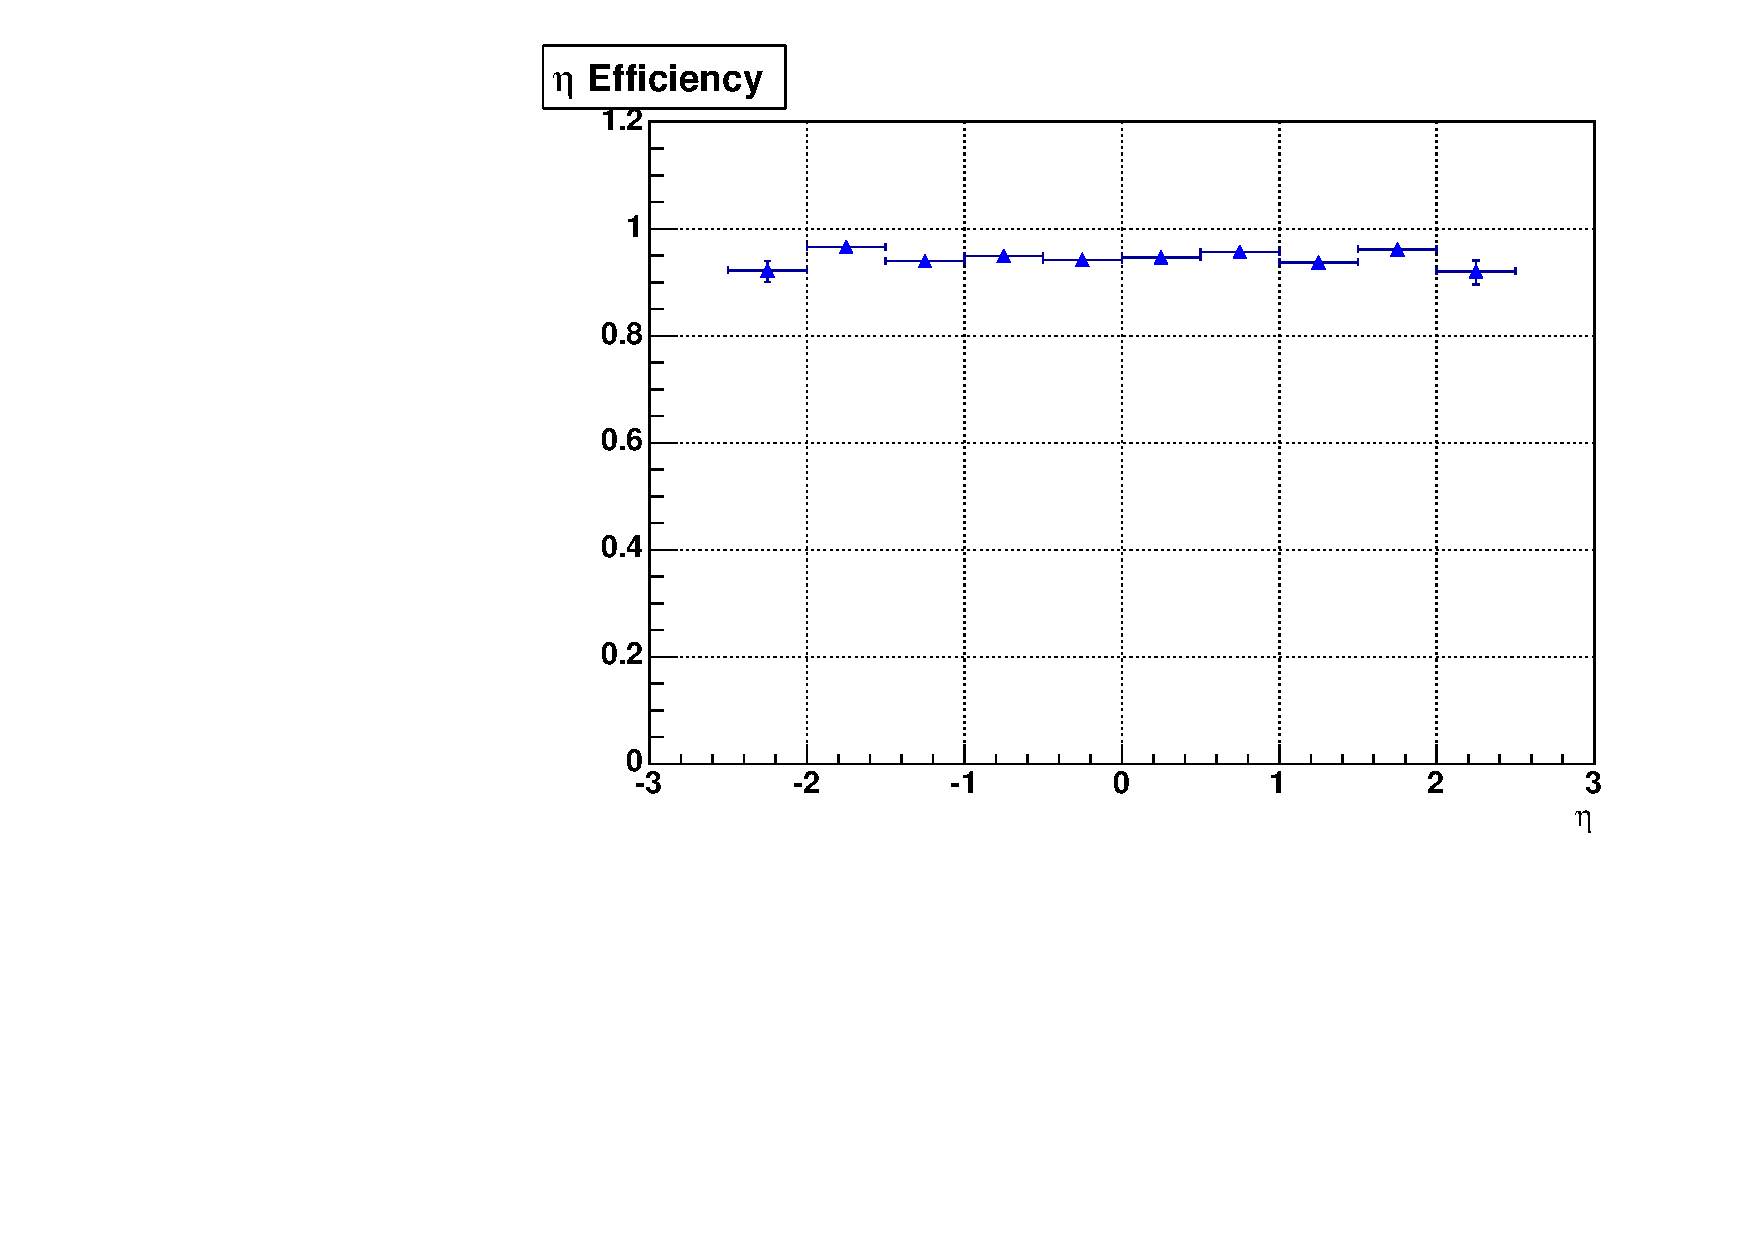
\includegraphics[width=\cmsFigWidth]{figures/soft_eta_eff}
    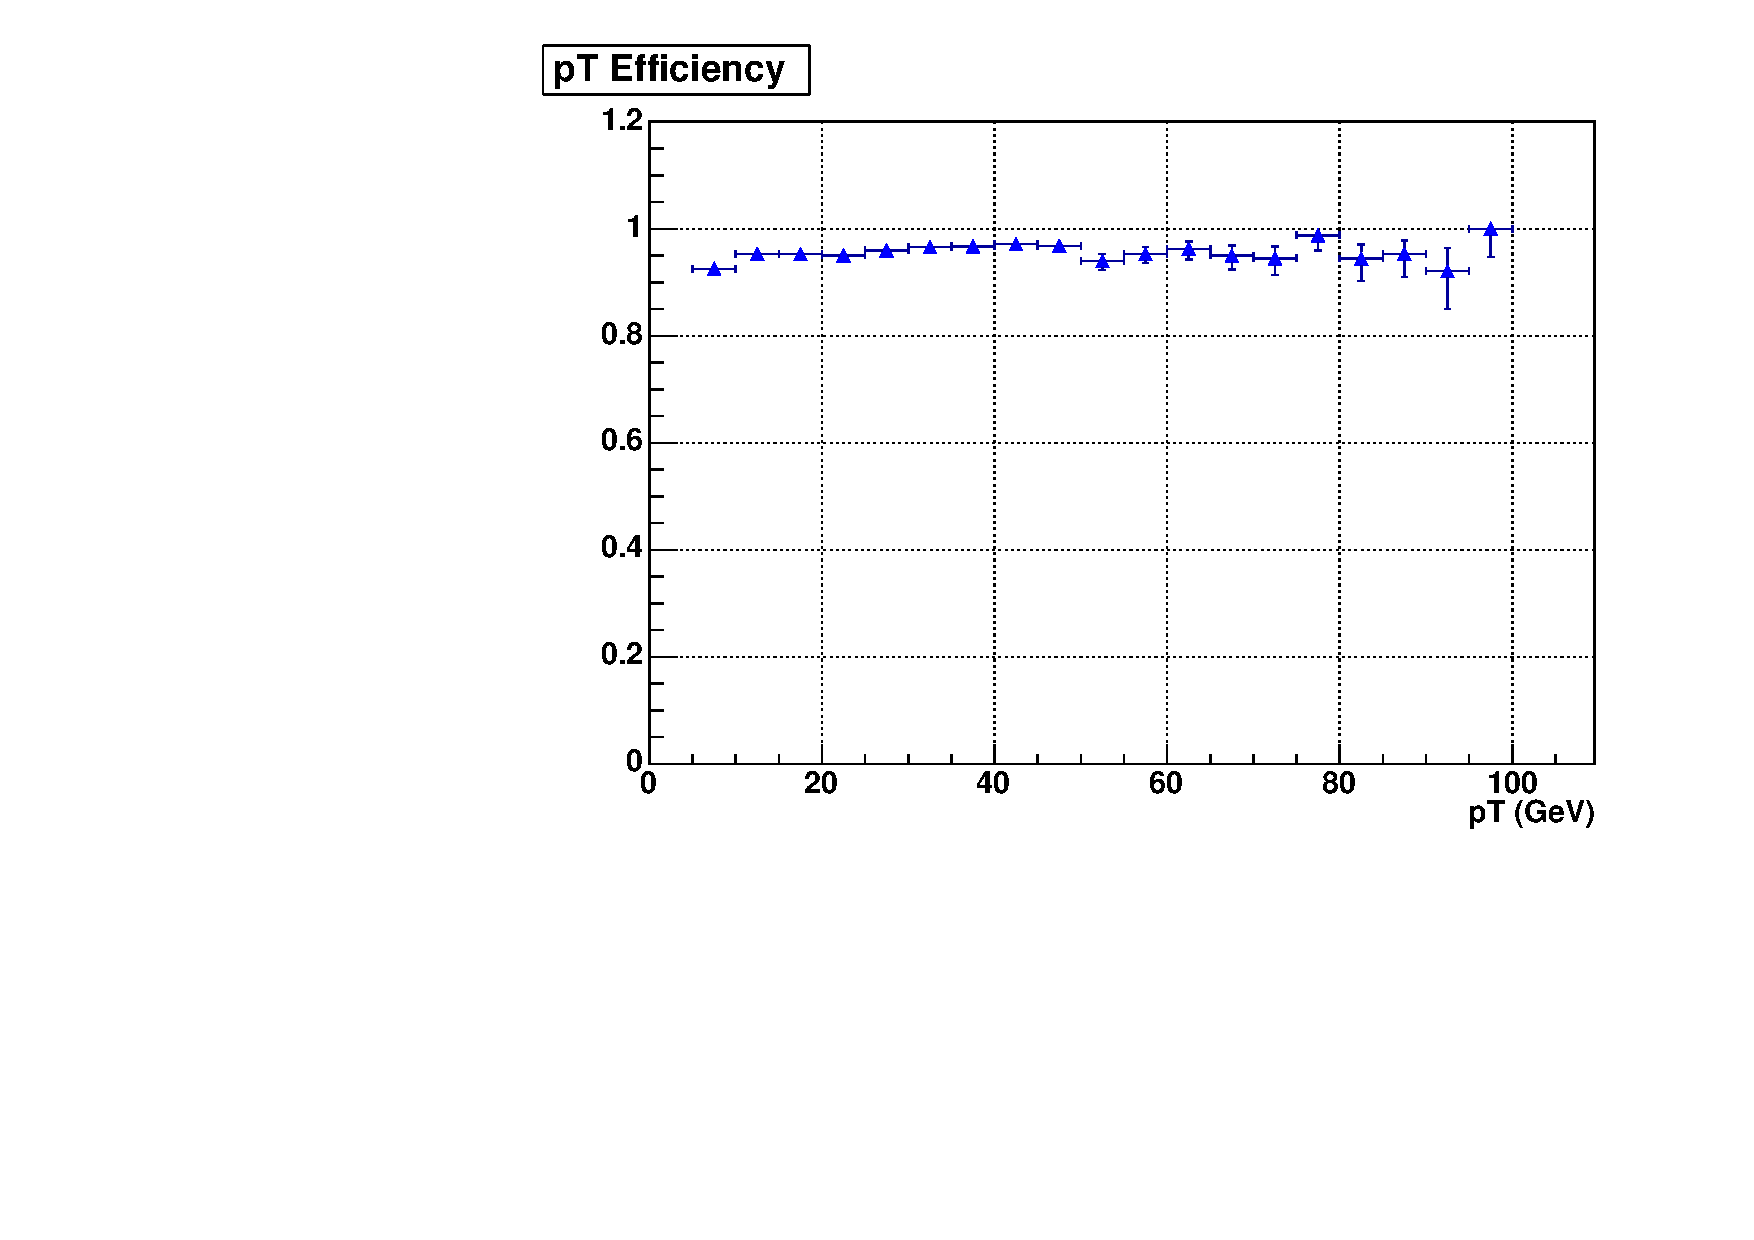
\includegraphics[width=\cmsFigWidth]{figures/soft_pt_eff}
    \caption{Soft muon efficiency as a function of $\eta$ (\cmsLeft) and $p_T$ (\cmsRight) in WH signal events. Errors are statistical only.}
    \label{fig:soft_muon}
  \end{center}
\end{figure}

The WH soft muon efficiency is $\sim$95\% across a range of $\eta$ and $p_T$ and is in good qualitative agreement with soft muon efficiencies measured in CMS data $J\slash\psi\rightarrow\mu\mu$ events~\cite{1748-0221-7-10-P10002}.  As the MUO POG measured soft muon efficiency agrees with the value from $J\slash\psi\rightarrow\mu\mu$ simulation~\cite{CMS:muonrefeffstwiki} within the quoted error, the signal WH and ggH MC is not corrected for differences from data.  Instead, the MUO POG recommended error of 1.5\% is propagated to the error on the expected signal.

%HPS tau id efficiency (Minsoo)
\subsection{HPS tau\label{sec:HPS-id}}

The MC sample \texttt{/DYJetsToLL\_M-50\_TuneZ2star\_8TeV-madgraph-tarball/\\Summer12\_DR53X-PU\_S10\_START53\_V7A-v1/AODSIM} is used to calculate HPS tau efficiency on $Z\rightarrow\tau_{\mu}\tau_{\text{had}}$ events.  The $\tau_{\mu}$ leg of the $Z$ decay is required to fire \texttt{HLT\_IsoMu24\_eta2p1} and pass the trigger muon ID.  HPS decay mode finding and isolation efficiency are measured on the $\tau_{\text{had}}$ leg.  For WH signal events, in addition to the trigger muon ID described above, the HPS tau is required to be built from a jet cleaned of a soft muon (cf. Sec.~\ref{sec:evtsel-ditau}).

The $p_T$ distributions of gen-level taus matched to reconstructed HPS taus are shown in Figure~\ref{fig:gen_whtt} for the WH sample and Figure~\ref{fig:gen_ztt} for the $Z\rightarrow\tau\tau$ sample.  Gen-matching is performed in a cone of $\Delta$R = 0.3 around the reconstructed HPS tau.  Signal WH taus tend to be softer than $Z$ decay taus, yet their ID and isolation efficiencies are similar as shown below.

\begin{figure}[hbtp]
  \begin{center}
    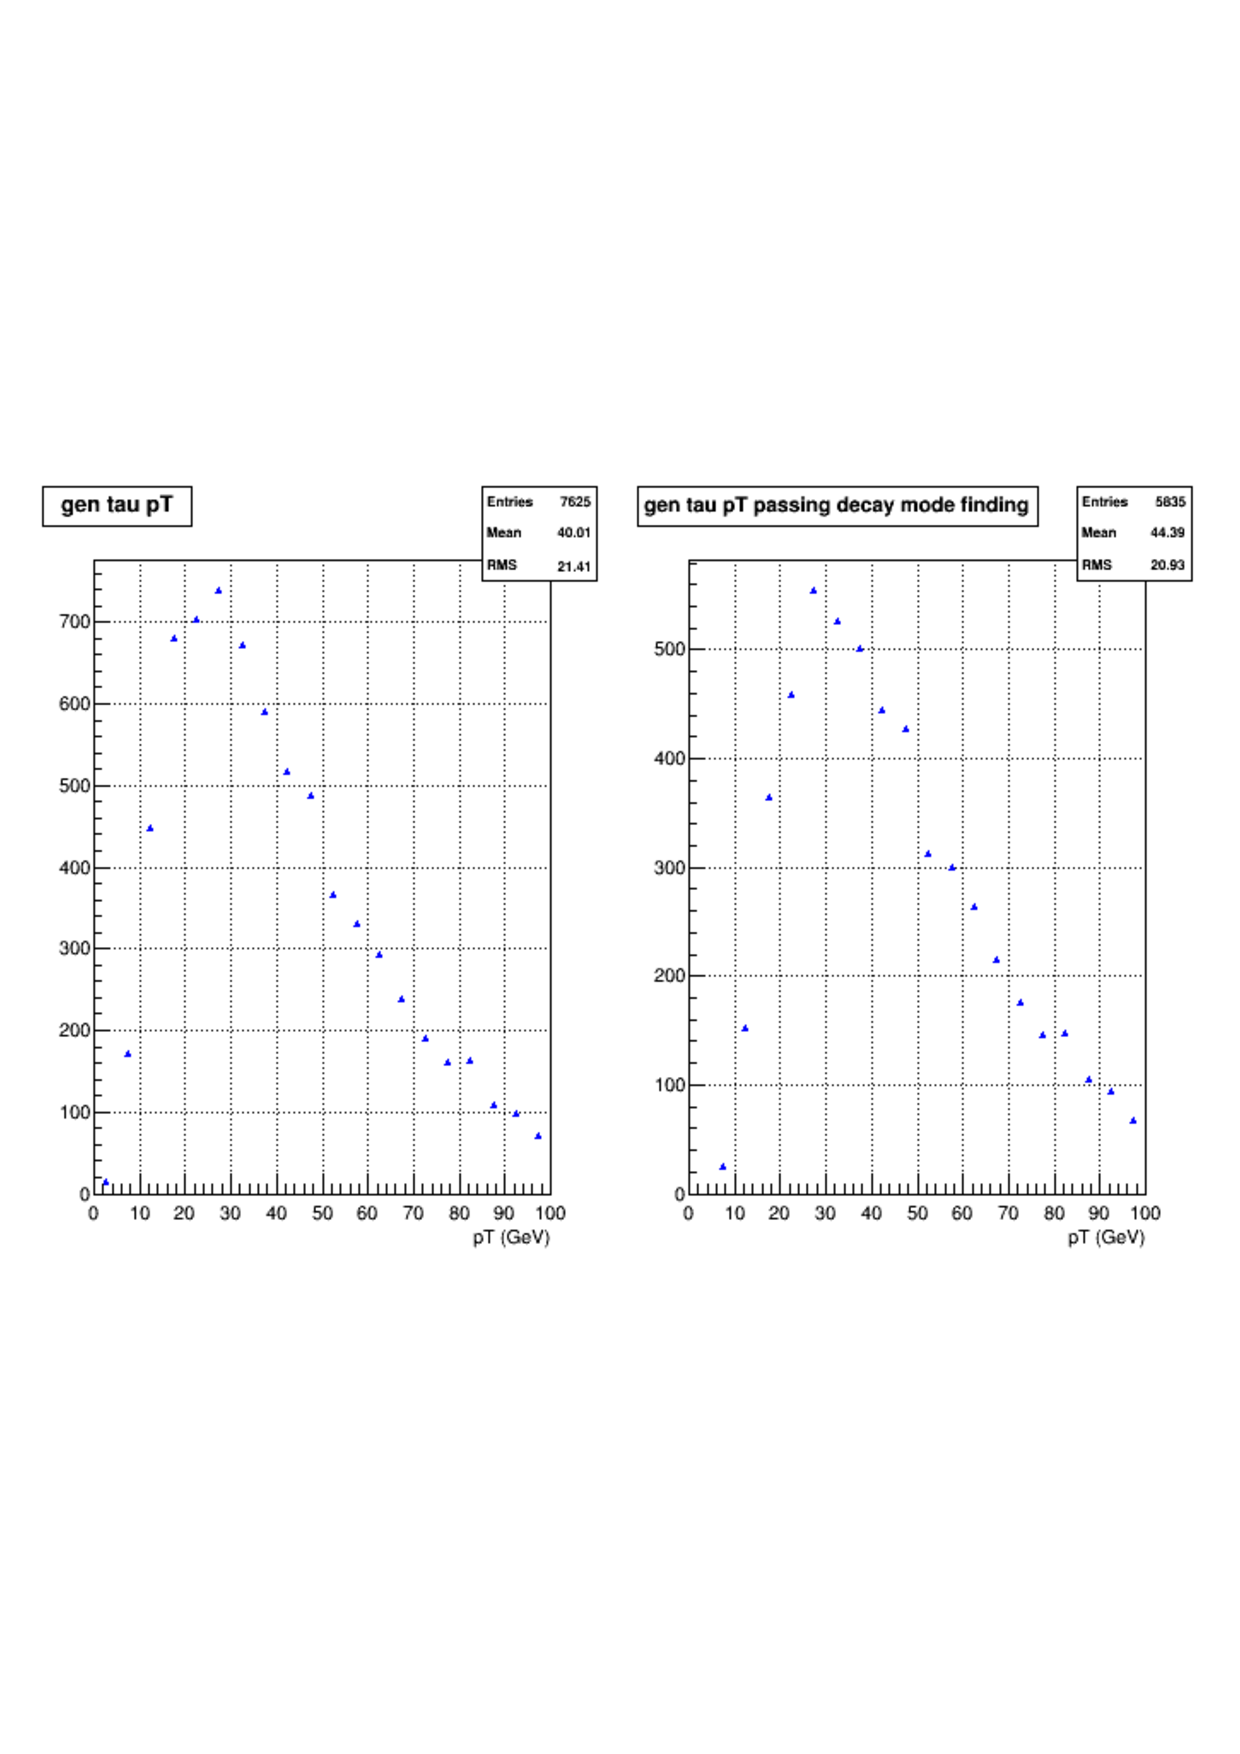
\includegraphics[width=\cmsFigWidth]{figures/pT_whtt_DMF}
    \caption{$p_T$ of gen taus from WH $\tau_{\mu}\tau_{\text{had}}$ pairs matched to reconstructed HPS taus with associated soft muons (cf. Sec.~\ref{sec:evtsel-ditau}).  Errors are statistical only.  (\cmsLeft) No discriminator requirement.  (\cmsRight) \texttt{DecayModeFinding} requirement.}
    \label{fig:gen_whtt}
  \end{center}
\end{figure}

\begin{figure}[hbtp]
  \begin{center}
    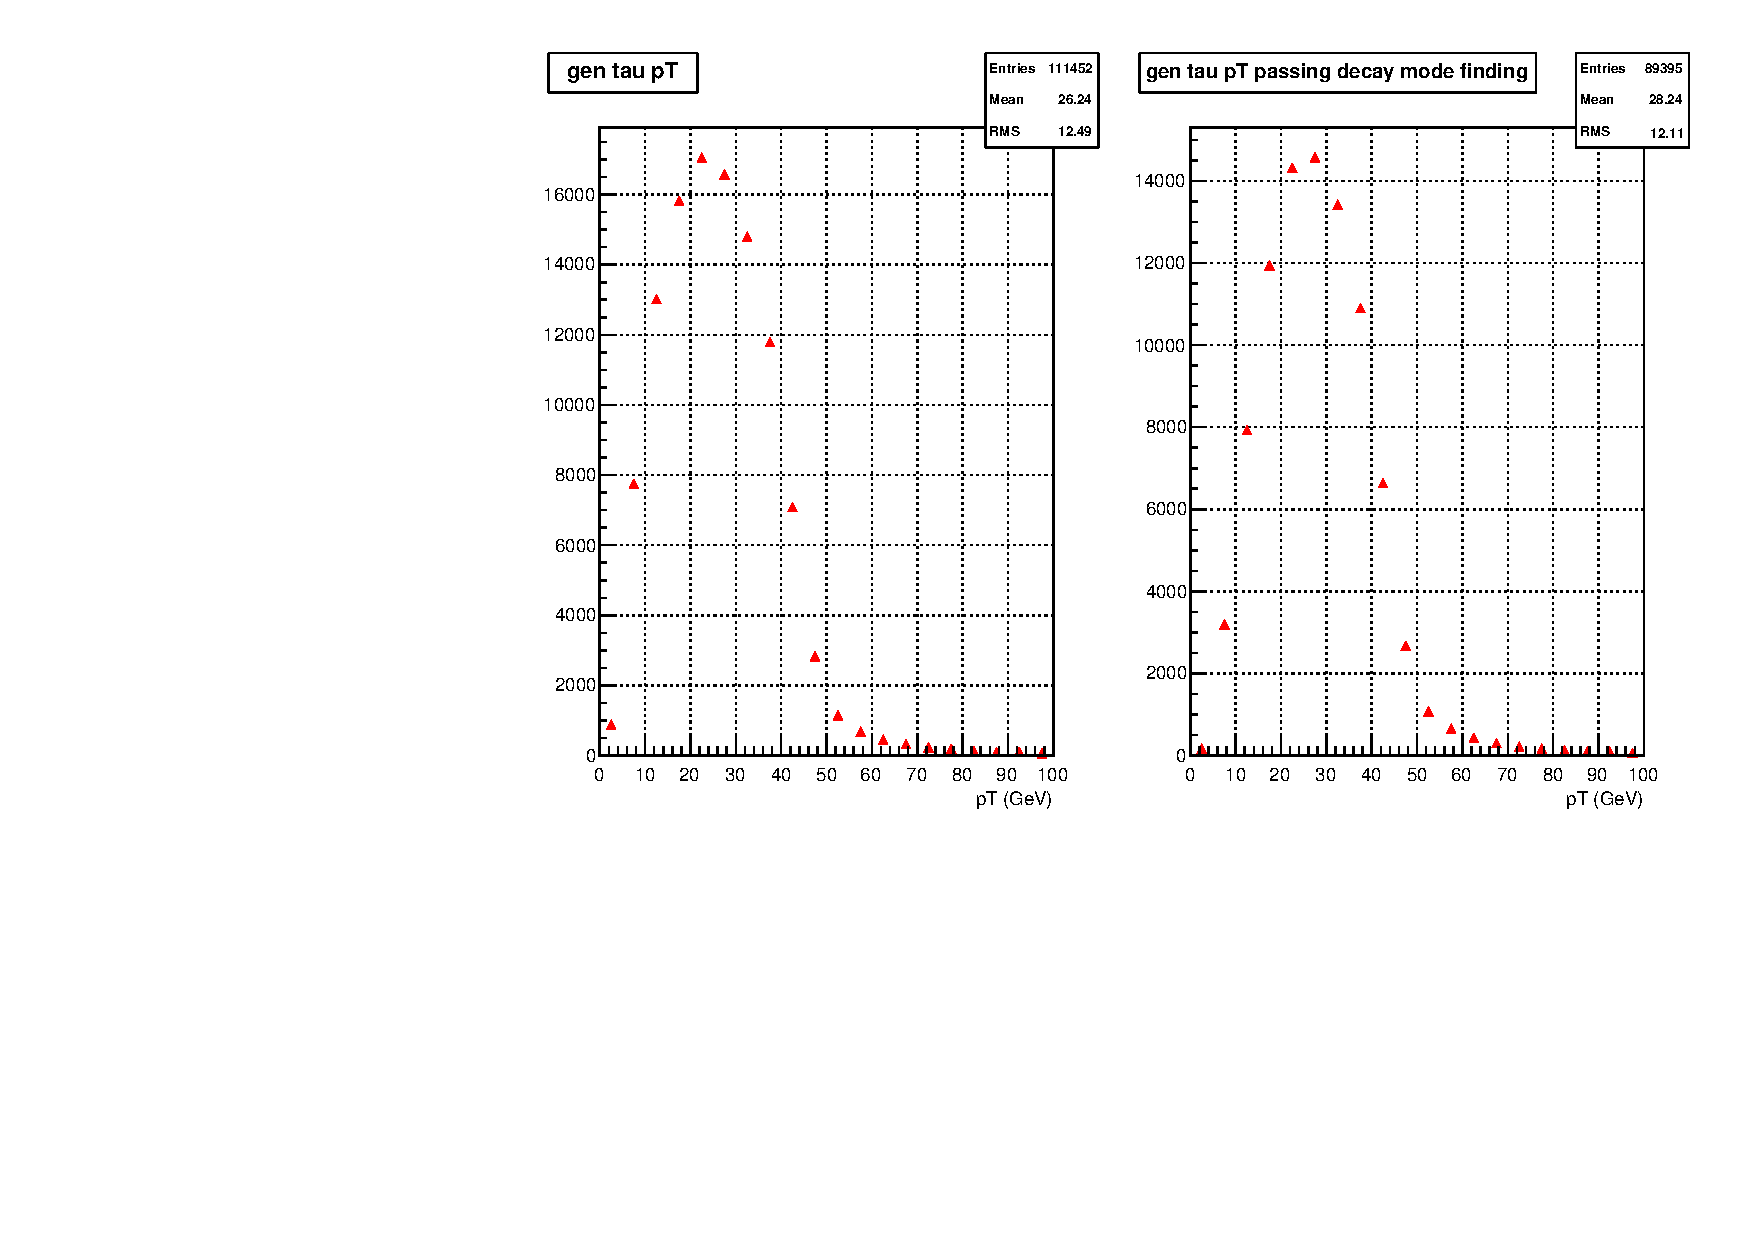
\includegraphics[width=\cmsFigWidth]{figures/gentau_pt_ztt_dmf}
    \caption{$p_T$ of gen taus from $Z\rightarrow\tau\tau$ decay matched to standard reconstructed HPS taus.  Errors are statistical only.  (\cmsLeft) No discriminator requirement.  (\cmsRight) \texttt{DecayModeFinding} requirement.}
    \label{fig:gen_ztt}
  \end{center}
\end{figure}

The decay mode finding efficiency $\epsilon_{\text{DMF}}$ = (number of gen-matched HPS taus in $\abs{\eta} <$ 2.4 passing the \texttt{DecayModeFinding} discriminator)/(number of gen-matched HPS taus in \abs{\eta} \textless\xspace 2.4) is shown for WHand $Z\rightarrow\tau\tau$ events in Figure~\ref{fig:eff_dmf} (\cmsLeft).  There is good agreement across a range of $\eta$ and $p_T$ between the simulated efficiency for signal boosted tau pair events reconstructed with the cleaning procedure described in Sec.~\ref{sec:evtsel-tauID} and $Z\rightarrow\tau_{\mu}\tau_{\text{had}}$ events.  In particular, the agreement is good even for relatively low tau $p_T$ ($<$ 20 GeV).  Similarly, the decay mode finding and isolation efficiency $\epsilon_{\text{DMF+iso}}$ = (number of gen-matched HPS taus in $\abs{\eta} <$ 2.4 passing the \texttt{DecayModeFinding} and \texttt{MediumCombinedIsolationDBSumPtCorr} discriminators)/(number of gen-matched HPS taus in $\abs{\eta} <$ 2.4) is shown in Figure~\ref{fig:eff_dmf_mi}. There is qualitative agreement with public TAU POG efficiencies for simulated $Z\rightarrow\tau\tau$ events~\cite{CMS:approvedTAUResults}.

\begin{figure}[hbtp]
  \begin{center}
    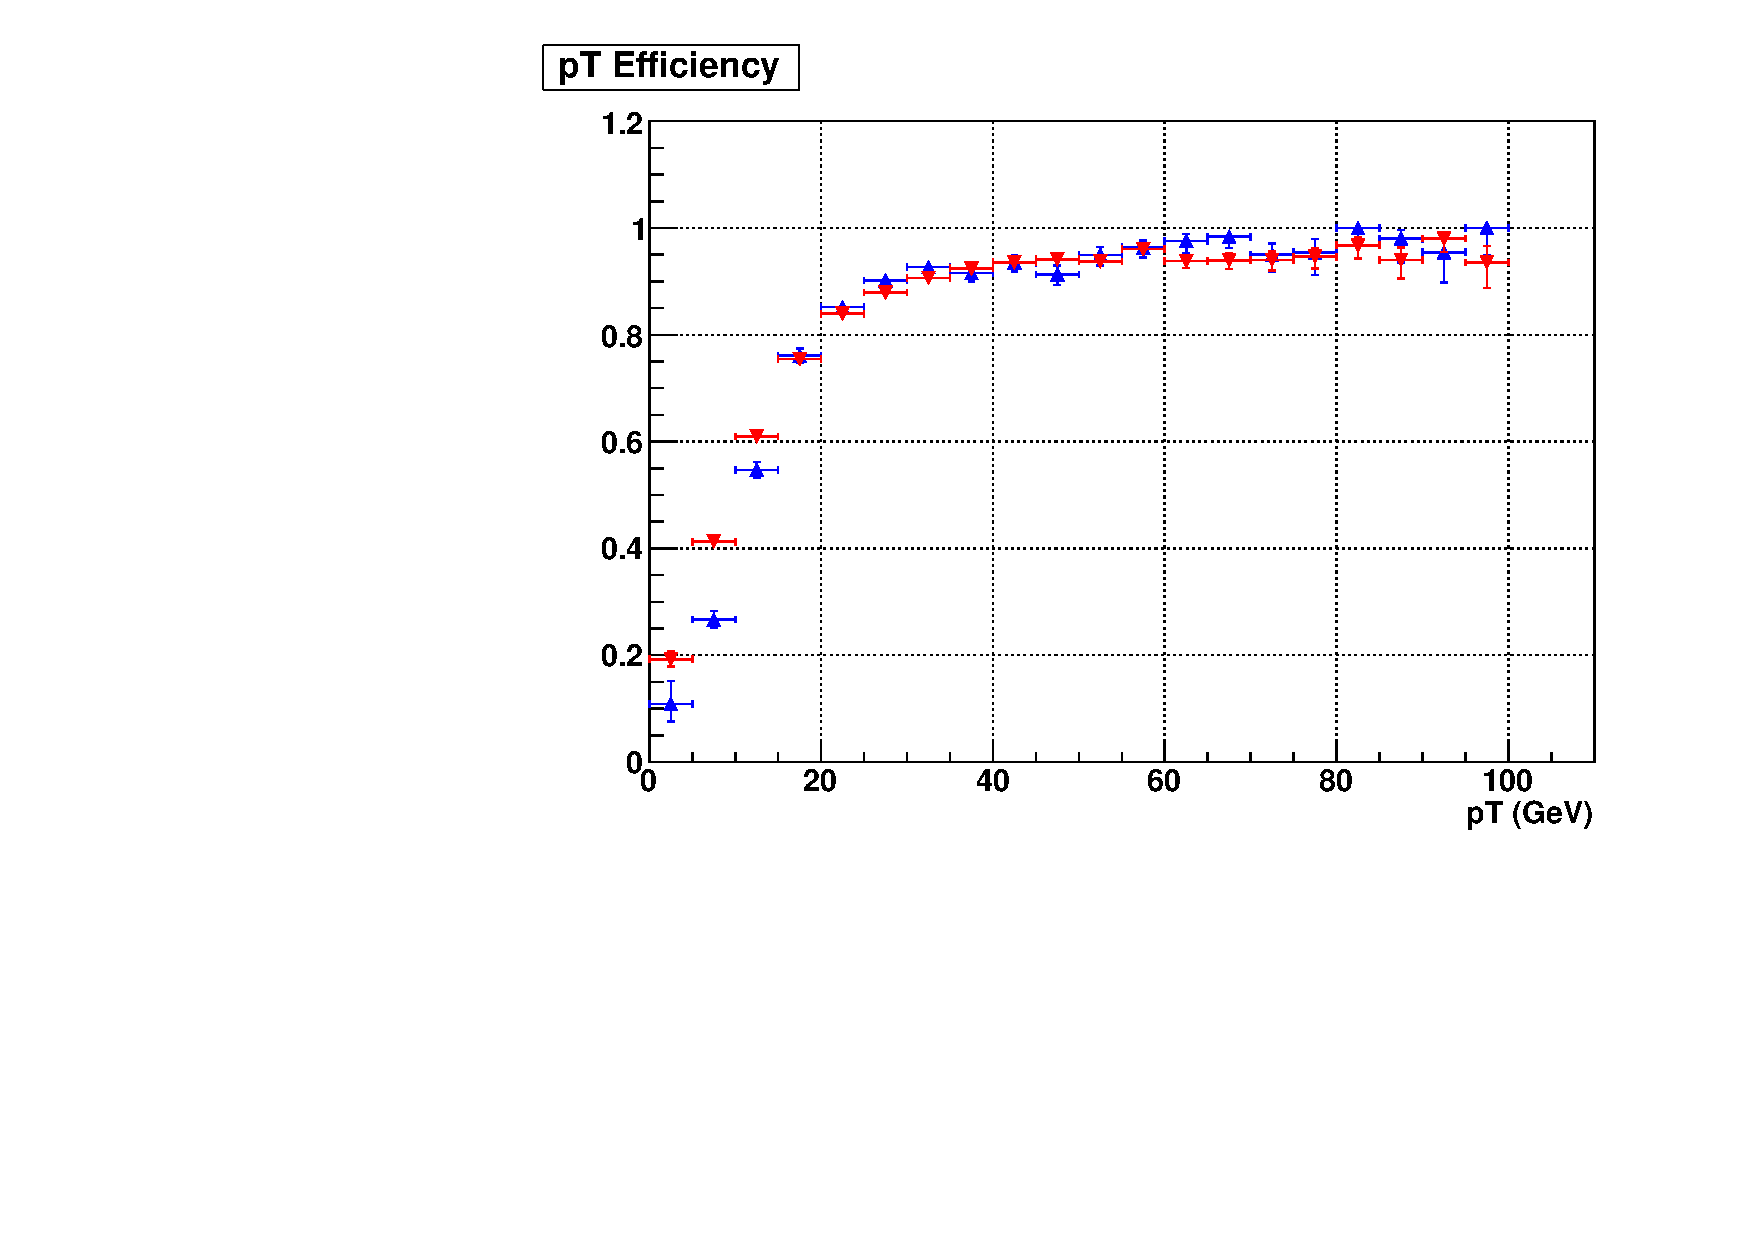
\includegraphics[width=\cmsFigWidth]{figures/gentau_dmf_pt}
    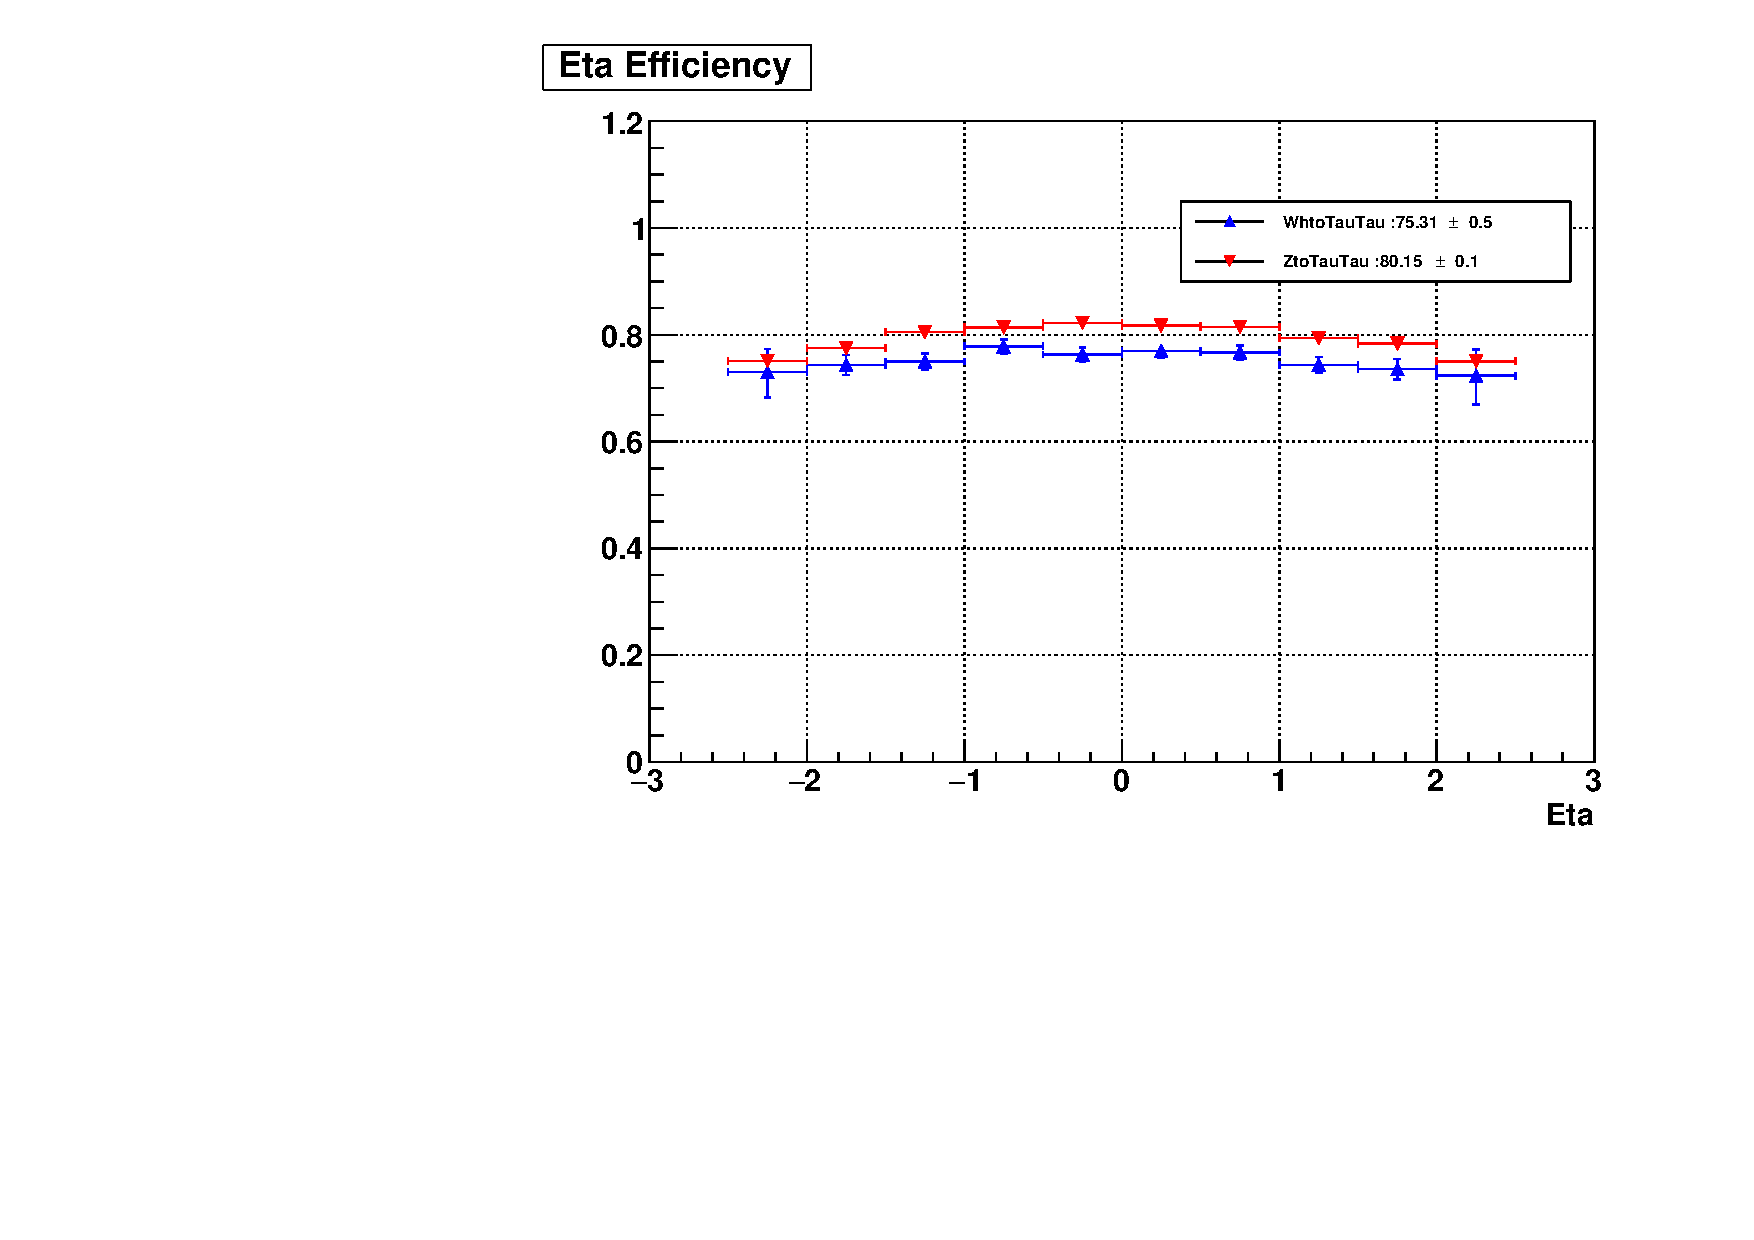
\includegraphics[width=\cmsFigWidth]{figures/gentau_dmf_eta}
    \caption{(\cmsLeft) HPS decay mode finding efficiency as a function of matched gen tau $p_T$. (\cmsRight) HPS decay mode finding efficiency as a function of matched gen tau $\eta$.  Signal HPS taus (blue) are reconstructed using the soft muon cleaning procedure described in this document, while taus from $Z$ decay (red) are reconstructed with standard HPS. Errors are statistical only.}
    \label{fig:eff_dmf}
  \end{center}
\end{figure}

\begin{figure}[hbtp]
  \begin{center}
    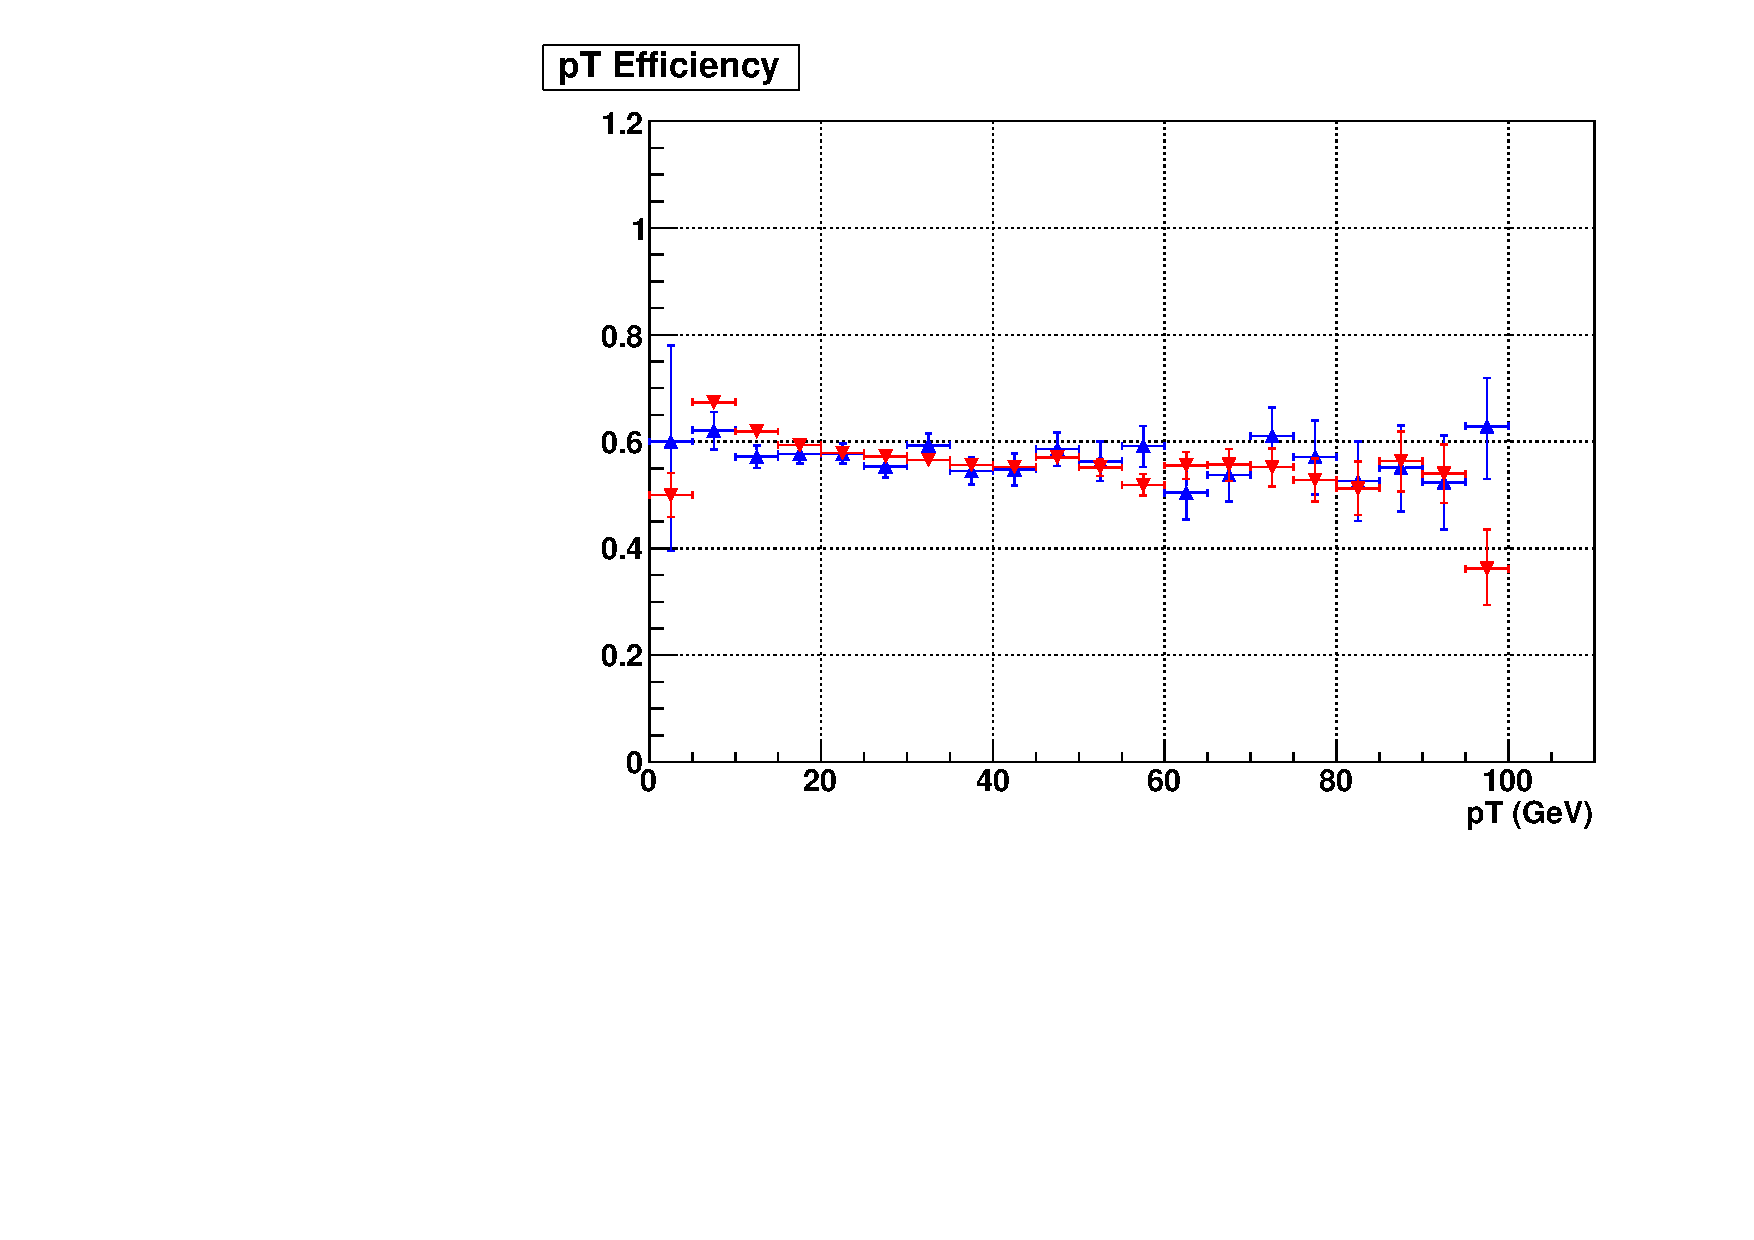
\includegraphics[width=\cmsFigWidth]{figures/gentau_dmfmi_pt}
    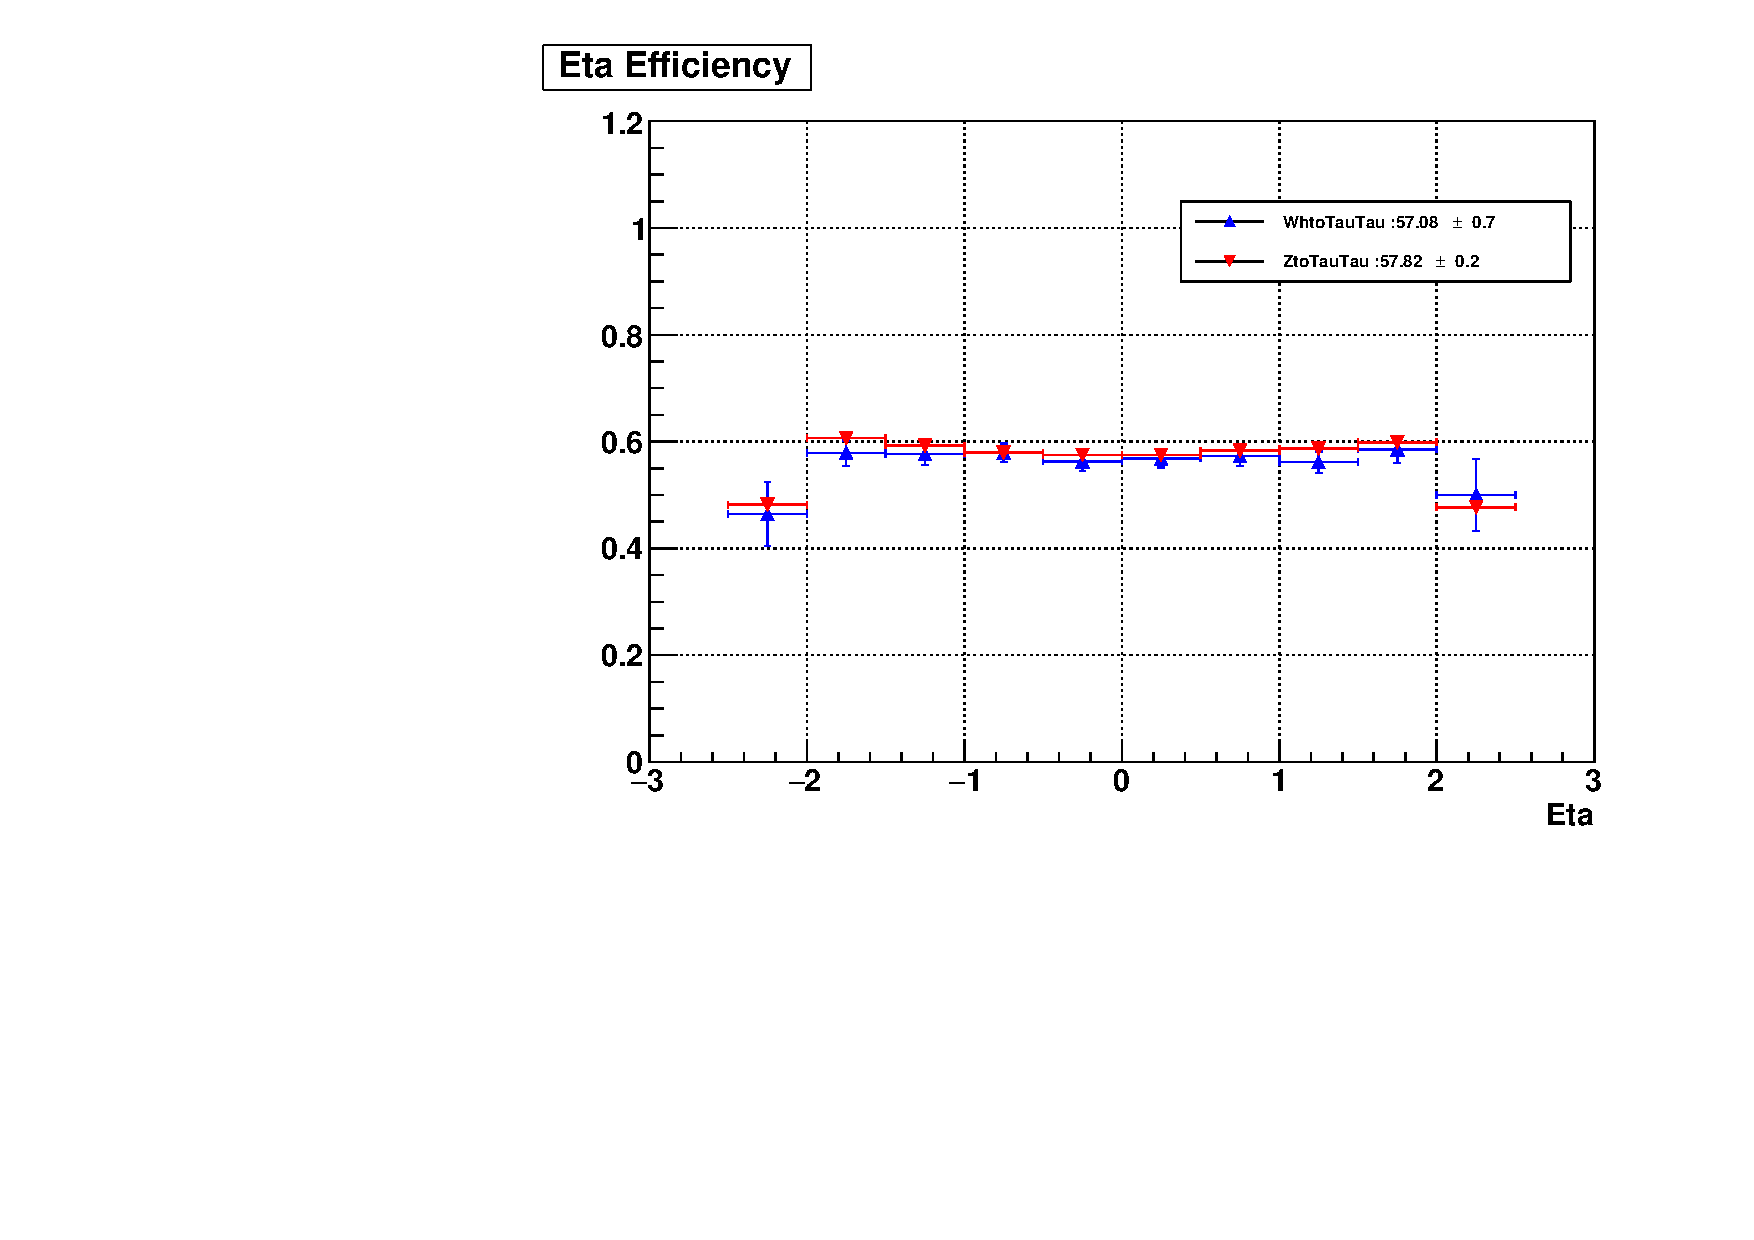
\includegraphics[width=\cmsFigWidth]{figures/gentau_dmfmi_eta}
    \caption{(\cmsLeft) HPS decay mode finding + medium combined isolation efficiency as a function of matched gen tau $p_T$. (\cmsRight) HPS decay mode finding efficiency as a function of matched gen tau $\eta$.  Signal HPS taus (blue) are reconstructed using the soft muon cleaning procedure described in this document, while taus from $Z$ decay (red) are reconstructed with standard HPS. Errors are statistical only.}
    \label{fig:eff_dmf_mi}
  \end{center}
\end{figure}

%As in the case of the soft muon, differences in the TAU POG approved HPS decay mode finding and isolation efficiencies between data and MC are within errors~\cite{CMS:tauuncertaintytwiki}, so instead of correcting the signal MC we simply propagate the recommended error of 6\% to the expected signal.
To cover discrepancies of up to about 10\% between the efficiencies in the signal and in $Z\rightarrow\tau_{\mu}\tau_{\text{had}}$, the TAU POG has recommended a conservative systematic of 10\% to apply to the HPS tau ID efficiency data-MC scale factor when a $p_T$ cut of 10 GeV is used. The $p_T$ cut used for the $\tau_{\text{had}}$ from the $\tau_{\mu}\tau_{\text{had}}$ object is 20 GeV; however, this efficiency study is still important because a $p_T$ cut of 10 GeV is applied to taus in the neighbouring lepton veto for the trigger muon (in order to have a better efficiency for the veto), and because future iterations of this search may explore the possibility of lowering the $p_T$ cut on the $\tau_{\text{had}}$ from $\tau_{\mu}\tau_{\text{had}}$ as well, as was originally intended.

Since the HPS tau ID efficiencies and scale factors have been validated by the TAU POG only down to 20 GeV, a study was done to reconstruct the \Z peak using HPS taus with $p_T$ between 10 and 20 GeV and to compare it to the $Z$ peak reconstructed from HPS taus with $p_T >$ 20 GeV, to assess the reliability of using taus with $p_T$ between 10 and 20 GeV. $Z\rightarrow\tau_{\mu}\tau_{\text{had}}$ events were selected in the MC sample \texttt{/DYJetsToLL\_M-50\_TuneZ2star\_8TeV-madgraph-tarball/\\Summer12\_DR53X-PU\_S10\_START53\_V7A-v1/AODSIM}; the $\tau_{\mu}$ leg of the \Z decay wass required to fire \texttt{HLT\_IsoMu24\_eta2p1}, pass the trigger muon ID, and be gen-matched to the $Z$ decay, while the gen-matched HPS tau was required to pass \texttt{DecayModeFinding} and \texttt{MediumCombined\\IsolationDBSumPtCorr} discriminators and a $p_T$ cut of either $>$ 20 GeV for the standard case, or between 10 and 20 GeV for the low-$p_T$ case of interest. As shown in Figure~\ref{fig:Zpeakstudy}, the Z peak looks normal for HPS tau $p_T$ \textgreater\xspace 20 GeV, and the Z peak shape for the low-$p_T$ range looks normal aside from being biased to a lower mean due to the lower HPS tau $p_T$ cut.

\begin{figure}[hbtp]
  \begin{center}
    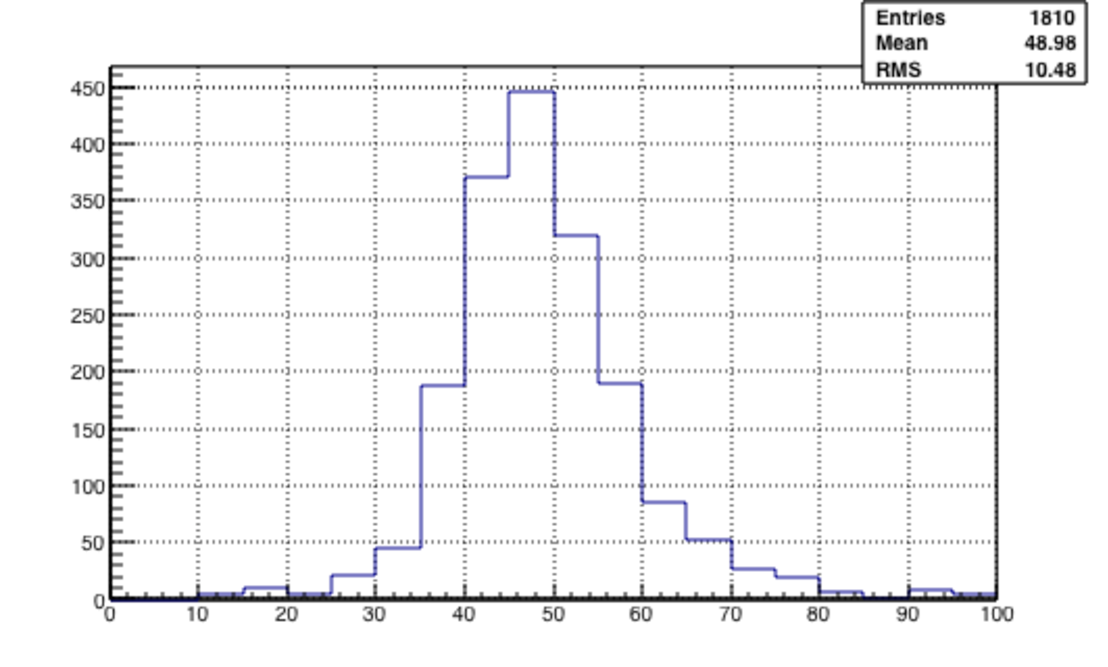
\includegraphics[width=\cmsFigWidth]{figures/gen_muhad_mass_1020}
    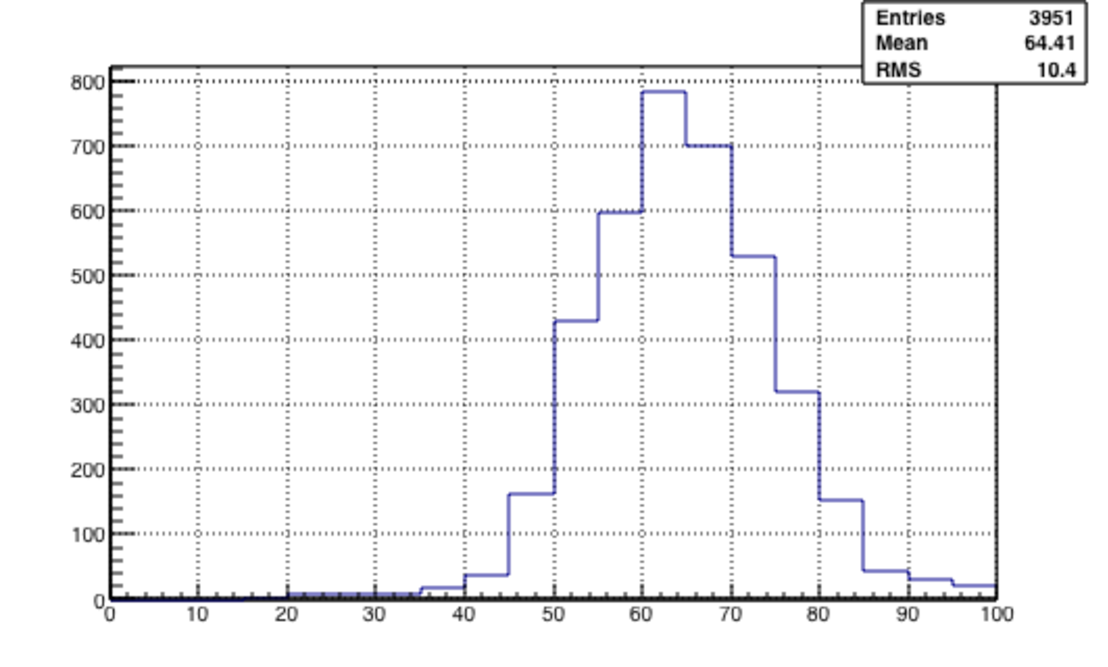
\includegraphics[width=\cmsFigWidth]{figures/gen_muhad_mass_20}
    \caption{Z peak reconstructed in a sample of Drell-Yan MC events. (\cmsLeft) HPS tau $p_T$ between 10 and 20 GeV. (\cmsRight) HPS tau $p_T <$ 20 GeV.}
    \label{fig:Zpeakstudy}
  \end{center}
\end{figure}
\chapter{Background modelling\label{sec:bkg}}

\section{Strategy\label{sec:bkg-strategy}}
Unlike the SM backgrounds, the new physics signal under study is characterized by the presence of a low mass $\tau_\mu\tau_\text{had}$ resonance.  Even though the $\tau$ decays cannot be fully reconstructed due to the neutrino decay products, the visible di-$\tau$ mass $m_{\mu+\text{had}}$ distribution can still be used to discriminate the signal resonance from background $\tau$ fakes.  Visible di-$\tau$ mass is defined as the invariant mass of the $\tau_\mu$ and $\tau_\text{had}$ objects described in Chapter~\ref{sec:evtsel}.

Figure~\ref{fig:muhad-mass-MC-region-A} shows the distribution of $m_{\mu+\text{had}}$ after the preselection has been applied for four signal models and all backgrounds.  While the signals have broad peaks around 4 GeV, the backgrounds peak at lower values and fall off sharply.

%show signal models with different values of ma1
\begin{figure}[hbtp]
  \begin{center}
    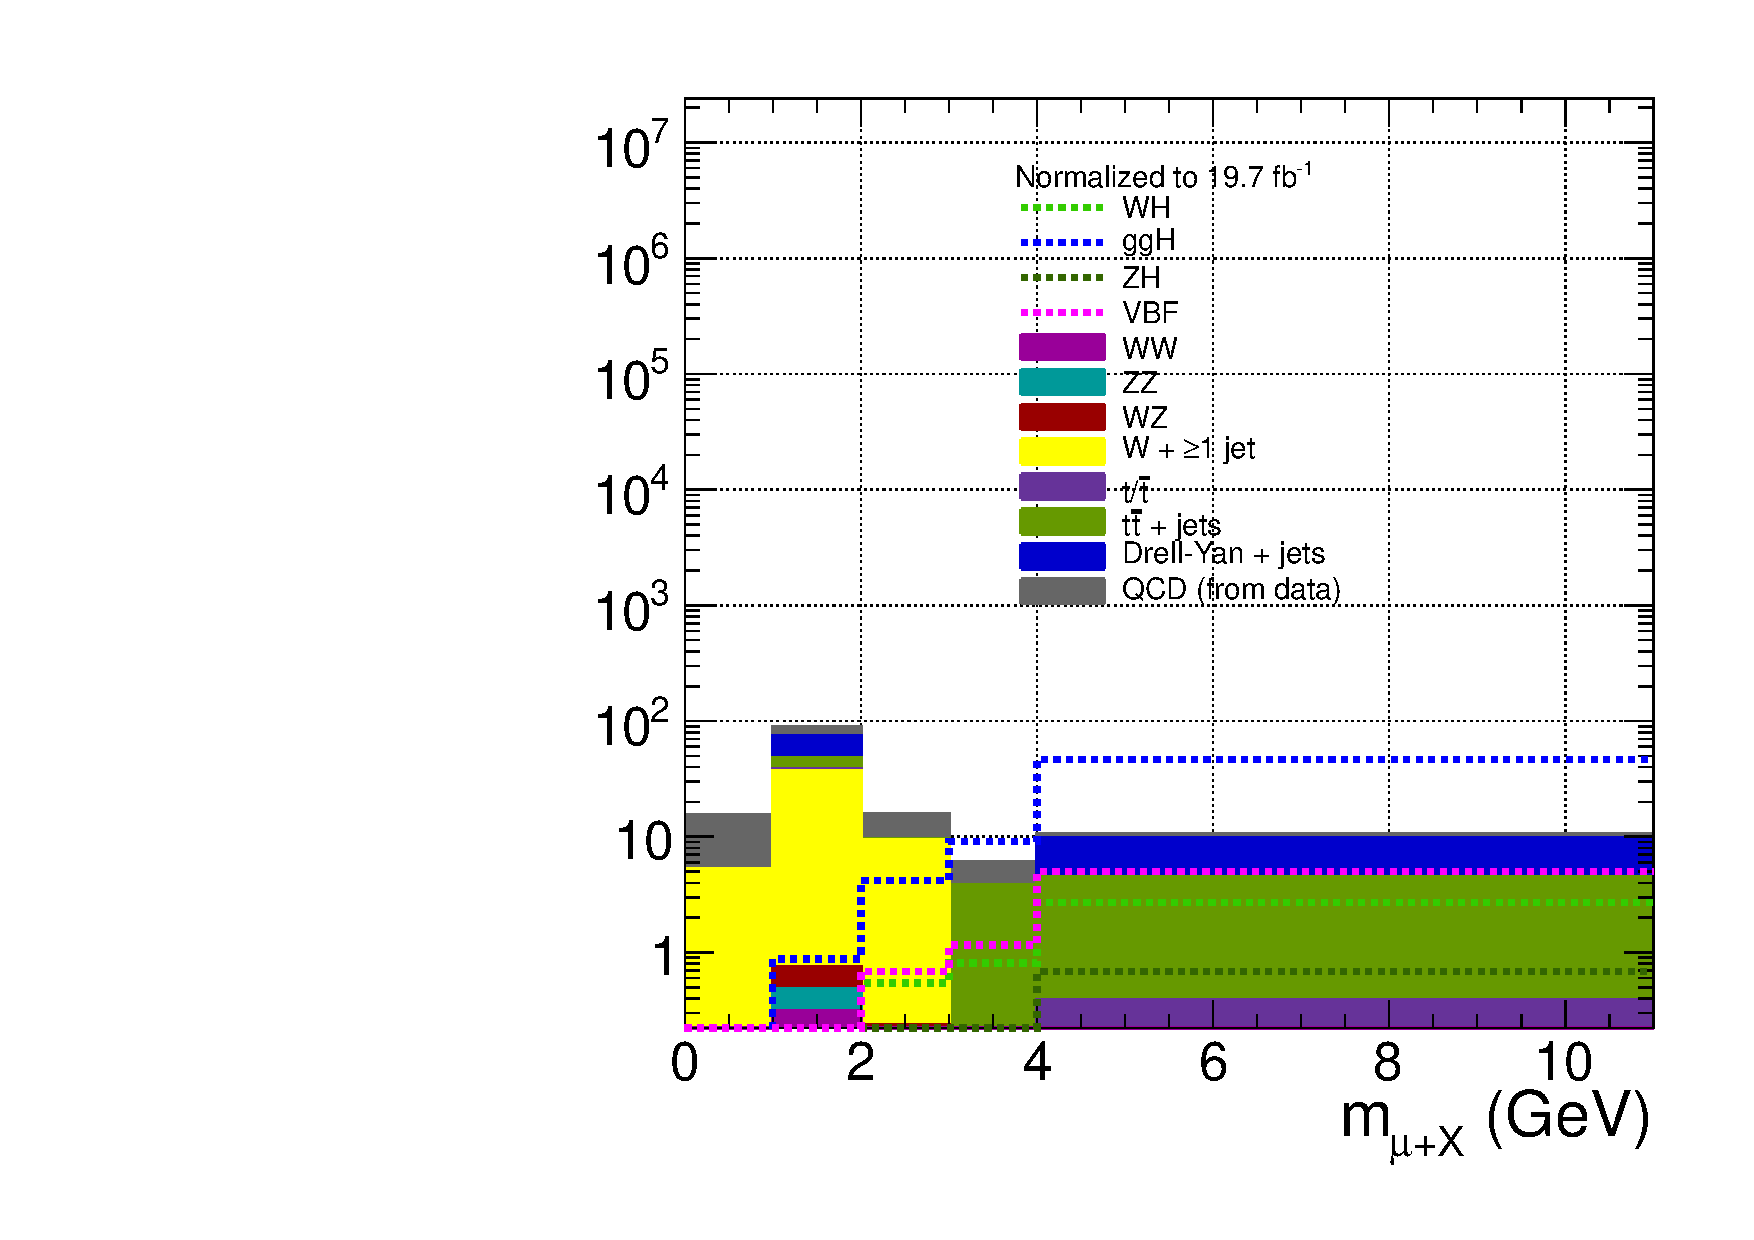
\includegraphics[width=\cmsFigWidth]{figures/sigVsBkg_muHadMass_lowMT_v87}
    \includegraphics[width=\cmsFigWidth]{figures/sigVsBkg_muHadMass_highMT_v87}
    \caption{$m_{\mu+\text{had}}$ distribution after the preselection has been applied for four signal models and all backgrounds. Normalized to 19.7 fb$^{-1}$. (\cmsLeft) Low-$M_{T}$ bin. (\cmsRight) High-$M_{T}$ bin.}
    \label{fig:muhad-mass-MC-region-A}
  \end{center}
\end{figure}

This search is a blinded counting experiment in the signal region (``region A'', cf. Figure~\ref{fig:regionsAB}) defined by the cuts described in Chapter~\ref{sec:evtsel} plus $m_{\mu+\text{had}}$ $\geq$ 4 GeV.  The value of 4 GeV has been roughly optimized for the signal-to-background ratio by eyeballing the distributions of $m_{\mu+\text{had}}$.

\begin{figure}[hbtp]
  \begin{center}
    \includegraphics[width=2\cmsFigWidth]{figures/ABCD_annotated_lowMT}
    \includegraphics[width=2\cmsFigWidth]{figures/ABCD_annotated_highMT}
    \caption{Schematic description of the signal and control regions in this search. Signal region A is defined by HPS $\tau$ isolation between 0 and 1 GeV, after events have passed all other preselection cuts detailed in Chapter~\ref{sec:evtsel}. Likewise, jet fake control region B is defined by HPS $\tau$ isolation between 1 and 5 GeV, after events have passed all other preselection cuts. Regions C and D, which are enriched in QCD events, including those with double $\mu$ decays, are identical to regions A and B respectively, except that the trigger $\mu$ fails the tight isolation requirement and the neighbouring lepton filter is not imposed.  (Top) Low $M_{\text{T}}$.  (Bottom) High $M_{\text{T}}$.}
    \label{fig:regionsAB}
  \end{center}
\end{figure}

The background shape is derived from a single control sample defined from the $\tau_{\text{had}}$ isolation sideband (``region B", cf. Figure~\ref{fig:regionsAB}).  It describes the shape of the background due to light jets or jets with single muon decays mis-reconstructed as $\tau_{\mu}\tau_{\text{had}}$ pairs (``jet fakes"). The signal-depleted sideband $m_{\mu+\text{had}}$ $<$ 2 GeV is used to normalize the $m_{\mu+\text{had}}$ distribution from the jet fake control sample to data passing all the cuts described in Chapter~\ref{sec:evtsel}.  This gives the nominal background prediction $N_{\text{fake; pred}}^{\text{A}}$ for signal region A; the final background prediction in the search region $m_{\mu+\text{had}} >$ 4 GeV is obtained from the normalized region B distribution in the manner described later in Sec.~\ref{sec:bkgs-jet-fake-unc}, which factors in uncertainties in the background composition.
%The $m_{\mu+\text{had}}$ distribution from the jet fake control sample is normalized to data passing all the cuts described in Sec.~\ref{sec:evt-sel}, but in the signal-depleted subsample with $m_{\mu+\text{had}}$ $<$ 2 GeV.  This gives the total background prediction $N_{\text{fake; pred}}^{\text{A}}$ for signal region A.

The expected SM backgrounds differ in the low and high $M_{T}$ regions; in the high $M_{T}$ region, trigger muons mostly come from $W$'s, while in the low $M_{T}$ region, they mostly come from jets (including heavy flavor). However, in both regions, the backgrounds are dominated by events with a $\tau_{\mu}\tau_{\text{had}}$ object. Thus, the assumption is made that the shape of the background $m_{\mu+\text{had}}$ distributions in regions A and B are similar. To account for possible differences in the scaling factors of different contributions between regions A and B, studies were done to investigate the changes in shape based on varying these assumptions.

%jet fake bkg
\section{Jet fake background estimation\label{sec:bkg-jetfake}}

The data control sample used for estimating the jet fake background (``region B'') is defined by all of the cuts in Chapter~\ref{sec:evtsel}, except that the tau isolation is required to be between 1 and 5 GeV.  Table~\ref{tab:regA-vs-regB-def} gives the cut values defining the search region (tau isolation $\le$ 1 GeV); the cuts defining the jet fake control region are all identical except for the cut on tau isolation.

\begin{table*}[htbH]
\begin{center}
\caption{Cut values defining the data search region A. The cuts defining the jet fake control region B are all identical, except that for having tau isolation $>$1 GeV \&\& $<$5 GeV.\label{tab:regA-vs-regB-def}}
\singlespacing
\begin{tabular}{ll}
\hline Variable & Search region \\% & Control region \\
\hline
HLT & \begin{tabular}[c]{@{}l@{}}\texttt{HLT\_IsoMu24\_eta2p1}\\\texttt{\_v[1-15]}\end{tabular} \\% & \begin{tabular}[c]{@{}l@{}}\texttt{HLT\_IsoMu24\_eta2p1}\\\texttt{\_v[1-15]}\end{tabular} \\
First muon $p_T$ & $>$25 GeV \\% & $>$25 GeV \\
First muon $|\eta|$ & $<$2.1 \\% & $<$2.1 \\
First muon ID (cf. Sec.~\ref{sec:evtsel-triggermu}) & Tight \\% & Tight \\
First muon rel. iso. (cf. Sec.~\ref{sec:evtsel-triggermu}) & $<$0.12 \\% & $<$0.12 \\
\DR(First muon, PF electron) (cf. Sec.~\ref{sec:evtsel-leptonveto}) & $>$0.4 \\% & $>$0.4 \\
\DR(First muon, soft muon) (cf. Sec.~\ref{sec:evtsel-leptonveto}) & $>$0.4 \\%& $>$0.4 \\
\DR(First muon, PF tau) (cf. Sec.~\ref{sec:evtsel-leptonveto}) & $>$0.4 \\%& $>$0.4 \\
\DR(first muon, HLT object) & $<$0.1 \\%& $<$0.1 \\
Second muon $p_T$ & $>$5 GeV \\%& $>$5 GeV \\
Second muon $\abs{\eta}$ & $<$2.1 \\%& $<$2.1 \\
Second muon ID (cf. Sec.~\ref{sec:evtsel-softmu}) & Soft \\%& Soft \\
Second muon $\neq$ first muon & True \\%& True \\
$q$(second muon) $\times$ $q$(first muon) & $>$0 \\%& $>$0 \\
\begin{tabular}[c]{@{}l@{}}Tau reco'd from jet cleaned \\of second muon (cf. Sec.~\ref{sec:evtsel-tauID})\end{tabular} & True \\%& True \\
Tau $p_T$ & $>$20 GeV \\%& $>$20 GeV \\
Tau $|\eta|$ & $<$2.3 \\%& $<$2.3 \\
Tau decay mode finding (cf. Sec.~\ref{sec:evtsel-tauID}) & True \\%& True \\
Tau isolation (cf. Sec.~\ref{sec:evtsel-tauID}) & Medium ($\le$1 GeV) \\%& $>$1 GeV \&\& $<$5 GeV \\
$q$(second muon) $\times$ $q$(tau) & =0 \\%& =0 \\
$\cPqb$ jet veto (cf. Sec.~\ref{sec:evtsel-bveto}) & CSVM \\%& CSVM \\
$d_{\text{z}}$($\tau_{\mu}$,PV) (cf. Sec.~\ref{sec:evtsel-dz}) & $<$0.5 cm \\%& $<$0.5 cm \\
$d_{\text{z}}$($\tau_{\text{had}}$,PV) (cf. Sec.~\ref{sec:evtsel-dz}) & $<$0.2 cm \\%& $<$0.2 cm \\
\hline
\end{tabular}
\end{center}
\end{table*}

%Subsection: Region B vs A shape validation
\subsection{Validation of similarity of background shapes in isolated and non-isolated tau regions\label{sec:bkgs-test-MC}}

For the Drell-Yan, $W$ + jets, top, and di-boson backgrounds, MC is used to check how well the jet fake control sample (region B) defined in Table~\ref{tab:regA-vs-regB-def} is expected to predict the shape of the $m_{\mu+\text{had}}$ distribution due to jet fakes in the search sample (region A).  For each of the MC samples described in Table~\ref{tab:MCBkg}, comparisons of the shapes of the $m_{\mu+\text{had}}$ distributions between samples of events passing the search region (A) cuts and those passing the control region (B) cuts are shown in Figures~\ref{fig:MC-regA-vs-regB-main-lowMT} and~\ref{fig:MC-regA-vs-regB-secondary-lowMT} for the low-$M_{\text{T}}$ bin and in Figures~\ref{fig:MC-regA-vs-regB-main-highMT} and~\ref{fig:MC-regA-vs-regB-secondary-highMT} for the high-$M_{\text{T}}$ bin. These figures show only the shape comparisons for the individual background sources without any information about their relative ratios in regions A and B; to validate the similarity of the overall background shapes in regions A and B, a comparison of the sum of the MC backgrounds is shown in Figures~\ref{fig:MC-regA-vs-regB-lowMT} and~\ref{fig:MC-regA-vs-regB-highMT}.

\begin{figure}[hbtp]
  \begin{center}
    \includegraphics[width=0.8\cmsFigWidth]{figures/isoVsNonIsoTaus_DY_lowMT_v87}
    \includegraphics[width=0.8\cmsFigWidth]{figures/isoVsNonIsoTaus_WNJets_lowMT_v87}
    \includegraphics[width=0.8\cmsFigWidth]{figures/isoVsNonIsoTaus_TTJets_lowMT_v87}
    \caption{$m_{\mu+\text{had}}$ distributions in the low-$M_{\text{T}}$ bin, normalized to one, for MC events passing the search region selection (black) and the jet fake control region selection (purple).  The small plots beneath the main plots show the ratio of the control region distribution to the search region distribution.  Errors are statistical only.  (\cmsLeft) Drell-Yan.  (Middle) $W$ + $\ge$1 jet.  (\cmsRight) $t\bar{t}$.}
    \label{fig:MC-regA-vs-regB-main-lowMT}
  \end{center}
\end{figure}

\begin{figure}[hbtp]
  \begin{center}
    \includegraphics[width=0.6\cmsFigWidth]{figures/isoVsNonIsoTaus_SingleTop_lowMT_v87}
    \includegraphics[width=0.6\cmsFigWidth]{figures/isoVsNonIsoTaus_WW_lowMT_v87}
    \includegraphics[width=0.6\cmsFigWidth]{figures/isoVsNonIsoTaus_WZ_lowMT_v87}
    \includegraphics[width=0.6\cmsFigWidth]{figures/isoVsNonIsoTaus_ZZ_lowMT_v87}
    \caption{$m_{\mu+\text{had}}$ distributions in the low-$M_{\text{T}}$ bin, normalized to one, for MC events passing the search region selection (black) and the jet fake control region selection (purple).  The small plots beneath the main plots show the ratio of the control region distribution to the search region distribution.  Errors are statistical only.  (\cmsLeft) Single top.  (Middle \cmsLeft) WW.  (Middle \cmsRight) WZ.  (\cmsRight) ZZ.}
    \label{fig:MC-regA-vs-regB-secondary-lowMT}
  \end{center}
\end{figure}

\begin{figure}[hbtp]
  \begin{center}
    \includegraphics[width=0.8\cmsFigWidth]{figures/isoVsNonIsoTaus_DY_highMT_v87}
    \includegraphics[width=0.8\cmsFigWidth]{figures/isoVsNonIsoTaus_WNJets_highMT_v87}
    \includegraphics[width=0.8\cmsFigWidth]{figures/isoVsNonIsoTaus_TTJets_highMT_v87}
    \caption{$m_{\mu+\text{had}}$ distributions in the high-$M_{\text{T}}$ bin, normalized to one, for MC events passing the search region selection (black) and the jet fake control region selection (purple).  The small plots beneath the main plots show the ratio of the control region distribution to the search region distribution.  Errors are statistical only.  (\cmsLeft) Drell-Yan.  (Middle) $W$ + $\ge$1 jet.  (\cmsRight) $t\bar{t}$.}
    \label{fig:MC-regA-vs-regB-main-highMT}
  \end{center}
\end{figure}

\begin{figure}[hbtp]
  \begin{center}
    \includegraphics[width=0.6\cmsFigWidth]{figures/isoVsNonIsoTaus_SingleTop_highMT_v87}
    \includegraphics[width=0.6\cmsFigWidth]{figures/isoVsNonIsoTaus_WW_highMT_v87}
    \includegraphics[width=0.6\cmsFigWidth]{figures/isoVsNonIsoTaus_WZ_highMT_v87}
    \includegraphics[width=0.6\cmsFigWidth]{figures/isoVsNonIsoTaus_ZZ_highMT_v87}
    \caption{$m_{\mu+\text{had}}$ distributions in the high-$M_{\text{T}}$ bin, normalized to one, for MC events passing the search region selection (black) and the jet fake control region selection (purple).  The small plots beneath the main plots show the ratio of the control region distribution to the search region distribution.  Errors are statistical only.  (\cmsLeft) Single top.  (Middle \cmsLeft) WW.  (Middle \cmsRight) WZ.  (\cmsRight) ZZ.}
    \label{fig:MC-regA-vs-regB-secondary-highMT}
  \end{center}
\end{figure}

\begin{figure}[hbtp]
  \begin{center}
    \includegraphics[width=\cmsFigWidth]{figures/MCClosure_lowMT_v87}
    \includegraphics[width=\cmsFigWidth]{figures/MCClosure_linear_lowMT_v87}
    \caption{Comparison of the $m_{\mu+\text{had}}$ distribution for the sum of the simulated backgrounds (all except QCD multi-jets) in the low-$M_{\text{T}}$ bin in the signal region A (blue) with the same distribution in the sideband control region B (red), which is used to model the total background distribution in region A.  The search region distribution is normalized to 19.7 fb$^{-1}$, while the control region distribution is normalized to the area of the search region distribution.  The small plots beneath the main plots show the ratio of the search region distribution to the control region distribution.  Errors are statistical only.  (\cmsLeft) Log scale for y axis.  (\cmsRight) Linear scale for y axis.}
    \label{fig:MC-regA-vs-regB-lowMT}
  \end{center}
\end{figure}

\begin{figure}[hbtp]
  \begin{center}
    \includegraphics[width=\cmsFigWidth]{figures/MCClosure_highMT_v87}
    \includegraphics[width=\cmsFigWidth]{figures/MCClosure_linear_highMT_v87}
    \caption{Comparison of the $m_{\mu+\text{had}}$ distribution for the sum of the simulated backgrounds (all except QCD multi-jets) in the low-$M_{\text{T}}$ bin in the signal region A (blue) with the same distribution in the sideband control region B (red), which is used to model the total background distribution in region A.  The search region distribution is normalized to 19.7 fb$^{-1}$, while the control region distribution is normalized to the area of the search region distribution.  The small plots beneath the main plots show the ratio of the search region distribution to the control region distribution.  Errors are statistical only.  (\cmsLeft) Log scale for y axis.  (\cmsRight) Linear scale for y axis.}
    \label{fig:MC-regA-vs-regB-highMT}
  \end{center}
\end{figure}

In the high-$M_{\text{T}}$ bin, where the main backgrounds are $W$ + jets and $t\bar{t}$, the total $m_{\mu+\text{had}}$ shape from simulation is consistent with the total region B shape within statistical errors separately for the $W$ + jets and $t\bar{t}$ samples (Figs.~\ref{fig:MC-regA-vs-regB-main-highMT} (middle) and~\ref{fig:MC-regA-vs-regB-main-highMT} (\cmsRight)).  In the low-$M_{\text{T}}$ bin, where the main backgrounds are QCD di-jets (no MC simulation available) and Drell-Yan + jets, the consistency between regions A and B separately for each MC sample is not as good.

%Subsection: qcd control regions
\subsection{QCD-enriched control regions in data\label{sec:bkgs-qcd-control}}

Two cross-checks are done to establish that the background from jets with double muon decays or isolated di-muon resonances (``resonances") is negligible.  For these cross checks, two other control samples, defined from the trigger muon isolation sideband (``region C" and ``region D'', cf. Figure~\ref{fig:regionsAB}), are used.  Since the trigger muon is required to be non-isolated, these regions are enriched in QCD di-jets, including heavy flavor jets with leptonic decays.  In the $m_{\mu+\text{had}}$ region around the $J\slash\psi$ mass, $\tau_{\mu}\tau_{\text{had}}$ resonances arise from $J\slash\psi\rightarrow\mu\mu$ decays where one muon fakes a tau.  In the $m_{\mu+\text{had}}$ region around the $\Upsilon$ mass, $\tau_{\mu}\tau_{\text{had}}$ resonances arise from real $\Upsilon\rightarrow\tau_{\mu}\tau_{\text{had}}$ decays.  In addition, jets may have two semileptonic decays to muons.  The first cross check, described in Section~\ref{sec:bkgs-resonances}, utilizes a fit around the $J\slash\psi$ mass to extract the $J\slash\psi$ component, while the second, described in Section~\ref{sec:bkgs-3-muon}, uses an independent control sample of three-muon events.

Data control regions C (isolated $\tau_{\mu}\tau_{\text{had}}$, non-isolated trigger muon) and D (non-isolated $\tau_{\mu}\tau_{\text{had}}$, non-isolated trigger muon, cf. Fig.~\ref{fig:regionsAB}) are also used to model the QCD di-jet backgrounds in regions A and B for the purpose of checking whether data with non-isolated taus (D) can accurately model data with isolated taus (C). The QCD shape in region A is taken from region C, defined by the trigger muon isolation sideband of the signal region (cf. Figure~\ref{fig:regionsAB}).  The predicted QCD $\tau_{\mu}\tau_{\text{had}}$ mass distribution in region A, denoted $f_{\text{A}}^{\text{QCD}}(m_{\mu+\text{had}})$, is given by

\begin{equation}
\label{eq:f-A-QCD}
f_{\text{A}}^{\text{QCD}}(m_{\mu+\text{had}}) = R_{\text{A}}^{\text{QCD}}\cdot f_{\text{C}}(m_{\mu+\text{had}})
\end{equation}

where

\begin{equation}
\label{eq:R-A-QCD}
R_{\text{A}}^{\text{QCD}} = [\int_{0}^{3 GeV}(f_{\text{B}}^{\text{data}}(m_{\mu+\text{had}}) - f_{\text{B}}^{\text{MC}}(m_{\mu+\text{had}}))dm_{\mu+\text{had}}]/[\int_{0}^{3 GeV}f_{\text{D}}(m_{\mu+\text{had}})dm_{\mu+\text{had}}]
\end{equation}

and $f_{\text{C}}(m_{\mu+\text{had}})$ is the $\tau_{\mu}\tau_{\text{had}}$ mass distribution in region C data.  In other words, the region C data distribution is normalized by a factor similar to that in Eq.~\ref{eq:R-B-QCD}, except that the integral runs from 0 to 3 GeV instead of 0 to infinity.

This procedure assumes that the QCD $m_{\mu+\text{had}}$ distributions in regions C and D have similar, compatible shapes. Analogously to the shape comparisons in regions A and B for the non-QCD background sources in simulation, a comparison of regions C and D is shown in Figure~\ref{fig:regs-C-vs-D}.  The agreement is reasonable, especially in the low $M_{\text{T}}$ bin for $m_{\mu+\text{had}} \geq$ 2 GeV.

\begin{figure}[hbtp]
  \begin{center}
    \includegraphics[width=\cmsFigWidth]{figures/regCDataVsRegDData_lowMT}
    \includegraphics[width=\cmsFigWidth]{figures/regCDataVsRegDData_highMT}
    \caption{$m_{\mu+\text{had}}$ distributions for data events in QCD-enriched regions C and D.  The region D distribution is normalized such that $N_{\text{C}}(m_{\mu+\text{had}} < 3\text{ }GeV)$ = $N_{\text{D}}(m_{\mu+\text{had}} < 3\text{ }GeV)$.  The small plots beneath the main plots show the ratio of the region C distribution to the region D distribution.  Errors are statistical only.  (\cmsLeft) Low $M_{\text{T}}$.  (\cmsRight) High $M_{\text{T}}$.}
    \label{fig:regs-C-vs-D}
  \end{center}
\end{figure}

%The same information is presented in tabular form in Table~\ref{tab:reg-ABCDRatios}.
To supplement the region A/B and C/D comparisons, Table~\ref{tab:reg-ABCDRatios} shows the number of events in the normalization sideband ($m_{\mu+\text{had}}$ $<$ 2 GeV) and search window ($m_{\mu+\text{had}}$ $\ge$ 4 GeV) for individual MC background sources and the data-driven QCD background in Regions A and B after the preselection, as well as the ratio of the number of normalization sideband events to the number of search window events in Regions A and B.

\begin{sidewaystable}
%\begin{table*}[htbH]
\begin{center}
\caption{Number of events after preselection in the normalization sideband ($m_{\mu+\text{had}}$ $<$ 2 GeV) and in the search window ($m_{\mu+\text{had}}$ $\ge$ 4 GeV) for individual MC backgrounds and the data-driven QCD background in Regions A and B, and the ratio of normalization sideband events to search window events.  The MC backgrounds are normalized to 19.7 fb$^{-1}$.  The data-driven QCD background shape for region A(B) comes from region C(D), while the normalization is discussed in Sections~\ref{sec:bkgs-test-MC} and~\ref{sec:bkgs-regB-data-MC}.\label{tab:reg-ABCDRatios}}
\singlespacing
\resizebox{\textwidth}{!}{\begin{tabular}{|l|c|c|c|c|c|c|}
\hline
& \multicolumn{3}{c}{Signal region (A)} & \multicolumn{3}{|c|}{Control region (B)} \\
\hline
$\text{M}_{\text{T}}$ $\le$ 50 GeV & $m_{\mu+\text{had}}$ $<$ 2 GeV & $m_{\mu+\text{had}}$ $\ge$ 4 GeV & $\frac{m_{\mu+\text{had}}\text{ }<\text{ }2\text{ }GeV}{m_{\mu+\text{had}}\text{ }\ge\text{ }4\text{ }GeV}$ & $m_{\mu+\text{had}}$ $<$ 2 GeV & $m_{\mu+\text{had}}$ $\ge$ 4 GeV & $\frac{m_{\mu+\text{had}}\text{ }<\text{ }2\text{ }GeV}{m_{\mu+\text{had}}\text{ }\ge\text{ }4\text{ }GeV}$ \\
\hline
WW & 0.315 $\pm$ 0.18 & 0 & --- & 0.726 $\pm$ 0.3 & 0 & --- \\
ZZ & 0.262 $\pm$ 0.096 & 0.108 $\pm$ 0.062 & 2.42 $\pm$ 1.7 & 0.998 $\pm$ 0.2 & 0.0421 $\pm$ 0.042 & 23.7 $\pm$ 24 \\
WZ & 0.344 $\pm$ 0.15 & 0 & --- & 1.58 $\pm$ 0.35 & 0 & --- \\
W + jets & 41.1 $\pm$ 10 & 0 & --- & 180 $\pm$ 26 & 0.367 $\pm$ 0.37 & 491 $\pm$ 5e+02 \\
Single top & 1.56 $\pm$ 0.8 & 0.278 $\pm$ 0.28 & 5.61 $\pm$ 6.3 & 4.47 $\pm$ 1.3 & 0.373 $\pm$ 0.32 & 12 $\pm$ 11 \\
$t\bar{t}$ & 9.76 $\pm$ 6.1 & 4.1 $\pm$ 4.1 & 2.38 $\pm$ 2.8 & 35.4 $\pm$ 11 & 0 & --- \\
Drell-Yan + jets & 26.8 $\pm$ 11 & 5.25 $\pm$ 3.7 & 5.1 $\pm$ 4.1 & 110 $\pm$ 22 & 5.92 $\pm$ 4.3 & 18.5 $\pm$ 14 \\
QCD (from data) & 24.9 $\pm$ 7 & 0.89 $\pm$ 0.7 & 28 $\pm$ 23 & 117 $\pm$ 30 & 7.23 $\pm$ 2.8 & 16.2 $\pm$ 7.5 \\
Tot. bkg. (MC + data-driven QCD) & 105 $\pm$ 17 & 10.6 $\pm$ 5.6 & 9.88 $\pm$ 5.4 & 450 $\pm$ 46 & 13.9 $\pm$ 5.1 & 32.3 $\pm$ 12 \\
Data & 122 & 7 & 17.4 & 430 & 22 & 19.5 \\
\hline
$\text{M}_{\text{T}}$ $\geq$ 50 GeV & $m_{\mu+\text{had}}$ $<$ 2 GeV & $m_{\mu+\text{had}}$ $\ge$ 4 GeV & $\frac{m_{\mu+\text{had}}\text{ }<\text{ }2\text{ }GeV}{m_{\mu+\text{had}}\text{ }\ge\text{ }4\text{ }GeV}$ & $m_{\mu+\text{had}}$ $<$ 2 GeV & $m_{\mu+\text{had}}$ $\ge$ 4 GeV & $\frac{m_{\mu+\text{had}}\text{ }<\text{ }2\text{ }GeV}{m_{\mu+\text{had}}\text{ }\ge\text{ }4\text{ }GeV}$ \\
\hline
WW & 0.472 $\pm$ 0.24 & 0 & --- & 3.66 $\pm$ 0.68 & 0 & --- \\
ZZ & 0.263 $\pm$ 0.1 & 0.145 $\pm$ 0.085 & 1.82 $\pm$ 1.3 & 0.723 $\pm$ 0.17 & 0.235 $\pm$ 0.097 & 3.08 $\pm$ 1.5 \\
WZ & 1.08 $\pm$ 0.28 & 0.404 $\pm$ 0.17 & 2.66 $\pm$ 1.3 & 2.71 $\pm$ 0.46 & 0.276 $\pm$ 0.14 & 9.85 $\pm$ 5.2 \\
W + jets & 74.6 $\pm$ 14 & 1.76 $\pm$ 1.5 & 42.4 $\pm$ 36 & 409 $\pm$ 39 & 6.29 $\pm$ 2.8 & 65 $\pm$ 29 \\
Single top & 2.5 $\pm$ 0.86 & 0 & --- & 15.5 $\pm$ 2.4 & 0.69 $\pm$ 0.43 & 22.5 $\pm$ 15 \\
$t\bar{t}$ & 17.7 $\pm$ 8 & 0 & --- & 59.9 $\pm$ 15 & 14.6 $\pm$ 8.6 & 4.11 $\pm$ 2.6 \\
Drell-Yan + jets & 11.7 $\pm$ 5.7 & 0.463 $\pm$ 0.46 & 25.4 $\pm$ 28 & 85.2 $\pm$ 18 & 0 & --- \\
QCD (from data) & 16.7 $\pm$ 15 & 0.49 $\pm$ 0.74 & 34 $\pm$ 60 & 56.5 $\pm$ 36 & 2.09 $\pm$ 2 & 27 $\pm$ 31 \\
Tot. bkg. (MC + data-driven QCD) & 125 $\pm$ 23 & 3.26 $\pm$ 1.7 & 38.3 $\pm$ 21 & 633 $\pm$ 59 & 24.1 $\pm$ 9.2 & 26.2 $\pm$ 10 \\
Data & 166 & 14 & 11.9 & 577 & 20 & 28.9 \\
\hline
\end{tabular}}
\end{center}
%\end{table*}
\end{sidewaystable}

%Subsection: understanding bkg
\subsection{Understanding background composition in jet fake control region (B)\label{sec:bkgs-regB-data-MC}}

In order to understand and have an independent validation of the background composition in the jet fake control region (B), comparisons of data and total non-QCD backgrounds from MC simulation are made for a number of different distributions characterizing region B.  The individual MC background distributions are normalized to the data luminosity of 19.7 fb$^{-1}$ using the cross sections given in Table~\ref{tab:MCBkg}, and event weights are applied to account for the different pileup distributions in data and MC according to the procedure described in Ref.~\cite{PU-Twiki}.  The available QCD MC does not provide enough events passing the control region selection to have any statistical power, so the QCD contribution is taken instead from the QCD-enriched control region in data defined by the trigger muon isolation sideband (``region D'', cf. Figure~\ref{fig:regionsAB}) of the jet fake control region.  The predicted QCD $\tau_{\mu}\tau_{\text{had}}$ mass distribution in region B, denoted $f_{\text{B}}^{\text{QCD}}(m_{\mu+\text{had}})$, is given by

\begin{equation}
\label{eq:f-B-QCD}
f_{\text{B}}^{\text{QCD}}(m_{\mu+\text{had}}) = R_{\text{B}}^{\text{QCD}}\cdot f_{\text{D}}(m_{\mu+\text{had}})
\end{equation}

where

\begin{equation}
\label{eq:R-B-QCD}
R_{\text{B}}^{\text{QCD}} = [\int_{0}^{\infty}(f_{\text{B}}^{\text{data}}(m_{\mu+\text{had}}) - f_{\text{B}}^{\text{MC}}(m_{\mu+\text{had}}))dm_{\mu+\text{had}}]/[\int_{0}^{\infty}f_{\text{D}}(m_{\mu+\text{had}})dm_{\mu+\text{had}}]
\end{equation}

$f_{\text{D}}(m_{\mu+\text{had}})$ is the $\tau_{\mu}\tau_{\text{had}}$ mass distribution in region D data, $f_{\text{B}}^{\text{data}}(m_{\mu+\text{had}})$ is the $\tau_{\mu}\tau_{\text{had}}$ mass distribution in region B data, and $f_{\text{B}}^{\text{MC}}(m_{\mu+\text{had}})$ is the $\tau_{\mu}\tau_{\text{had}}$ mass distribution in region B MC.  In other words, the region D data distribution is normalized to the number of data events minus the sum of MC events in region B, where the MC sum is normalized to 19.7 fb$^{-1}$.  Figure~\ref{fig:QCDComparisonBD} shows the comparison of $m_{\mu+{\text{had}}}$ shapes between region D data and region B data minus total non-QCD background from simulation, which are generally consistent with each other within statistical errors.

\begin{figure}[hbtp]
  \begin{center}
    \includegraphics[width=\cmsFigWidth]{figures/muHadMassCanvas_regBDataMinusMCVsRegDData_lowMT}
    \includegraphics[width=\cmsFigWidth]{figures/muHadMassCanvas_regBDataMinusMCVsRegDData_highMT}
    \caption{Comparison of $m_{\mu+{\text{had}}}$ shapes between region D data and region B data minus total non-QCD backgrounds from simulation.  The region D distribution is normalized such that $N_{\text{D}}(m_{\mu+\text{had}} < 3\text{ }GeV)$ = $N_{\text{B}}^{\text{data - MC}}(m_{\mu+\text{had}} < 3\text{ }GeV)$.  (\cmsLeft) Low $M_{\text{T}}$. (\cmsRight) High $M_{\text{T}}$.}
    \label{fig:QCDComparisonBD}
  \end{center}
\end{figure}

Table~\ref{tab:regB-predictions} shows the breakdown of the expected SM contributions and observed data above $m_{\mu+\text{had}}$ = 4 GeV in the isolation sideband control region B, including statistical errors.  Figures~\ref{fig:regB-data-MC-nGoodVtx}-\ref{fig:regB-data-MC-tauMuPT} show some comparisons between region B data, region B MC, and the region B QCD prediction (which is taken from region D).

\begin{table*}[htbH]
\begin{center}
\caption{Expected SM events (from MC; QCD from region D data) and observed events above $m_{\mu+\text{had}}$ = 4 GeV in Region B.  The MC backgrounds are normalized to 19.7 fb$^{-1}$.  The QCD normalization is given by Eqs.~\ref{eq:f-B-QCD} and~\ref{eq:R-B-QCD}.\label{tab:regB-predictions}}
\begin{tabular}{lll}
\hline & $\text{M}_{\text{T}}$ $\le$ 50 GeV & $\text{M}_{\text{T}}$ $>$ 50 GeV \\
\hline
WW & 0 & 0 \\
ZZ & 0.0421 $\pm$ 0.042 & 0.235 $\pm$ 0.097 \\
WZ & 0 & 0.276 $\pm$ 0.14 \\
W + jets & 0.367 $\pm$ 0.37 & 6.29 $\pm$ 2.8 \\
Single top & 0.373 $\pm$ 0.32 & 0.69 $\pm$ 0.43 \\
$t\bar{t}$ & 0 & 14.6 $\pm$ 8.6 \\
Drell-Yan + jets & 5.92 $\pm$ 4.3 & 0 \\
QCD (from data) & 7.23 $\pm$ 2.8 & 2.09 $\pm$ 2 \\
\hline
Tot. expected SM & 13.9 $\pm$ 5.1 & 24.1 $\pm$ 9.2 \\
\hline
Data & 22 & 20 \\
\hline
\end{tabular}
\end{center}
\end{table*}

\begin{figure}[hbtp]
  \begin{center}
    \includegraphics[width=\cmsFigWidth]{figures/dataVsMCQCD_nGoodVtx_lowMT_v87}
    \includegraphics[width=\cmsFigWidth]{figures/dataVsMCQCD_nGoodVtx_highMT_v87}
    \caption{Distribution of the number of good reconstructed vertices for region B data (black points), region B total non-QCD backgrounds from MC (solid stacked histograms), and the QCD prediction from region D data (solid gray histogram).  A good reconstructed vertex is required to not be fake, have $>$4 degrees of freedom, have z position $\le$24 \cm, and have radial position $\le$2 \cm.  Errors are statistical only. (\cmsLeft) Low-$M_{\text{T}}$ bin. (\cmsRight) High-$M_{\text{T}}$ bin.}
    \label{fig:regB-data-MC-nGoodVtx}
  \end{center}
\end{figure}

\begin{figure}[hbtp]
  \begin{center}
    \includegraphics[width=\cmsFigWidth]{figures/dataVsMCQCD_MET_lowMT_v87}
    \includegraphics[width=\cmsFigWidth]{figures/dataVsMCQCD_MET_highMT_v87}
    \caption{\ETslash distribution for region B data (black points), region B total non-QCD backgrounds from MC (solid stacked histograms), and the QCD prediction from region D data (solid gray histogram).  Errors are statistical only. (\cmsLeft) Low-$M_{\text{T}}$ bin. (\cmsRight) High-$M_{\text{T}}$ bin.}
    \label{fig:regB-data-MC-MET}
  \end{center}
\end{figure}

\begin{figure}[hbtp]
  \begin{center}
    \includegraphics[width=\cmsFigWidth]{figures/dataVsMCQCD_WMuMT_lowMT_v87}
    \includegraphics[width=\cmsFigWidth]{figures/dataVsMCQCD_WMuMT_highMT_v87}
    \caption{Trigger muon $M_{\text{T}}$ distribution for region B data (black points), region B total non-QCD backgrounds from MC (solid stacked histograms), and the QCD prediction from region D data (solid gray histogram).  Errors are statistical only. The term ``$W$ muon'' in the label refers to the trigger muon, not necessarily a muon from a $W$ decay (as in the case of the $ggH$ signal, for instance).  (\cmsLeft) Low-$M_{\text{T}}$ bin. (\cmsRight) High-$M_{\text{T}}$ bin.}
    \label{fig:regB-data-MC-MT}
  \end{center}
\end{figure}

\begin{figure}[hbtp]
  \begin{center}
    \includegraphics[width=\cmsFigWidth]{figures/dataVsMCQCD_dPhiWMuMET_lowMT_v87}
    \includegraphics[width=\cmsFigWidth]{figures/dataVsMCQCD_dPhiWMuMET_highMT_v87}
    \caption{$\Delta\phi$(trigger muon, \ETslash) distribution for region B data (black points), region B total non-QCD backgrounds from MC (solid stacked histograms), and the QCD prediction from region D data (solid gray histogram).  Errors are statistical only. The term ``$W$ muon'' in the label refers to the trigger muon, not necessarily a muon from a $W$ decay (as in the case of the $ggH$ signal, for instance).  (\cmsLeft) Low-$M_{\text{T}}$ bin. (\cmsRight) High-$M_{\text{T}}$ bin.}
    \label{fig:regB-data-MC-dPhiWMuMET}
  \end{center}
\end{figure}

\begin{figure}[hbtp]
  \begin{center}
    \includegraphics[width=\cmsFigWidth]{figures/dataVsMCQCD_dPhiTauMuMET_lowMT_v87}
    \includegraphics[width=\cmsFigWidth]{figures/dataVsMCQCD_dPhiTauMuMET_highMT_v87}
    \caption{$\Delta\phi$($\tau$ muon, \ETslash) distribution for region B data (black points), region B total non-QCD backgrounds from MC (solid stacked histograms), and the QCD prediction from region D data (solid gray histogram).  Errors are statistical only. (\cmsLeft) Low-$M_{\text{T}}$ bin. (\cmsRight) High-$M_{\text{T}}$ bin.}
    \label{fig:regB-data-MC-dPhiTauMuMET}
  \end{center}
\end{figure}

\begin{figure}[hbtp]
  \begin{center}
    \includegraphics[width=\cmsFigWidth]{figures/dataVsMCQCD_mWMuTauMu_lowMT_v87}
    \includegraphics[width=\cmsFigWidth]{figures/dataVsMCQCD_mWMuTauMu_highMT_v87}
    \caption{Distribution of the invariant mass of the trigger muon and $\tau$ muon for region B data (black points), region B total non-QCD backgrounds from MC (solid stacked histograms), and the QCD prediction from region D data (solid gray histogram).  Errors are statistical only. (\cmsLeft) Low-$M_{\text{T}}$ bin. (\cmsRight) High-$M_{\text{T}}$ bin.}
    \label{fig:regB-data-MC-mWMuTauMu}
  \end{center}
\end{figure}

\begin{figure}[hbtp]
  \begin{center}
    \includegraphics[width=\cmsFigWidth]{figures/dataVsMCQCD_muHadMass_lowMT_v87}
    \includegraphics[width=\cmsFigWidth]{figures/dataVsMCQCD_muHadMass_highMT_v87}
    \caption{$m_{\mu+\text{had}}$ distribution for region B data (black points), region B total non-QCD backgrounds from MC (solid stacked histograms), and the QCD prediction from region D data (solid gray histogram).  Errors are statistical only. (\cmsLeft) Low-$M_{\text{T}}$ bin. (\cmsRight) High-$M_{\text{T}}$ bin.}
    \label{fig:regB-data-MC-muHadMass}
  \end{center}
\end{figure}

\begin{figure}[hbtp]
  \begin{center}
    \includegraphics[width=\cmsFigWidth]{figures/dataVsMCQCD_nAddlJetsPTGeq30_lowMT_v87}
    \includegraphics[width=\cmsFigWidth]{figures/dataVsMCQCD_nAddlJetsPTGeq30_highMT_v87}
    \caption{Number of anti-\kt R = 0.5 PF jets with L1FastL2L3~\cite{1748-0221-6-11-P11002} corrected $p_T >$ 30 GeVc. Distribution for region B data (black points), region B total non-QCD backgrounds from MC (solid stacked histograms), and the QCD prediction from region D data (solid gray histogram).  Errors are statistical only. (\cmsLeft) Low-$M_{\text{T}}$ bin. (\cmsRight) High-$M_{\text{T}}$ bin.}
    \label{fig:regB-data-MC-nAddlJetsPTGeq20}
  \end{center}
\end{figure}

\begin{figure}[hbtp]
  \begin{center}
    \includegraphics[width=\cmsFigWidth]{figures/dataVsMCQCD_muHadNchtrk1_lowMT_v87}
    \includegraphics[width=\cmsFigWidth]{figures/dataVsMCQCD_muHadNchtrk1_highMT_v87}
    \caption{Number of charged tracks with $p_T >$ 1 GeVc in the parent jet of the $\tau_{\mu}\tau_{\text{had}}$ object. Distribution for region B data (black points), region B total non-QCD backgrounds from MC (solid stacked histograms), and the QCD prediction from region D data (solid gray histogram).  Errors are statistical only. (\cmsLeft) Low-$M_{\text{T}}$ bin. (\cmsRight) High-$M_{\text{T}}$ bin.}
    \label{fig:regB-data-MC-muHadNchtrk1}
  \end{center}
\end{figure}

\begin{figure}[hbtp]
  \begin{center}
    \includegraphics[width=\cmsFigWidth]{figures/dataVsMCQCD_HT_lowMT_v87}
    \includegraphics[width=\cmsFigWidth]{figures/dataVsMCQCD_HT_highMT_v87}
    \caption{$p_T$ sum of the tau muon, hadronic tau, highest $p_T$ distinct jet, trigger muon, and \ETslash. Distribution for region B data (black points), region B total non-QCD backgrounds from MC (solid stacked histograms), and the QCD prediction from region D data (solid gray histogram).  Errors are statistical only. (\cmsLeft) Low-$M_{\text{T}}$ bin. (\cmsRight) High-$M_{\text{T}}$ bin.}
    \label{fig:regB-data-MC-tauMuTauHadJetWMuMETHT}
  \end{center}
\end{figure}

\begin{figure}[hbtp]
  \begin{center}
    \includegraphics[width=\cmsFigWidth]{figures/dataVsMCQCD_tauHadPT_lowMT_v87}
    \includegraphics[width=\cmsFigWidth]{figures/dataVsMCQCD_tauHadPT_highMT_v87}
   \caption{Hadronic tau $p_T$ distribution for region B data (black points), region B total non-QCD backgrounds from MC (solid stacked histograms), and the QCD prediction from region D data (solid gray histogram).  Errors are statistical only. (\cmsLeft) Low-$M_{\text{T}}$ bin. (\cmsRight) High-$M_{\text{T}}$ bin.}
    \label{fig:regB-data-MC-tauHadPT}
  \end{center}
\end{figure}

\begin{figure}[hbtp]
  \begin{center}
    \includegraphics[width=\cmsFigWidth]{figures/dataVsMCQCD_tauHadEta_lowMT_v87}
    \includegraphics[width=\cmsFigWidth]{figures/dataVsMCQCD_tauHadEta_highMT_v87}
    \caption{Hadronic tau $\eta$ distribution for region B data (black points), region B total non-QCD backgrounds from MC (solid stacked histograms), and the QCD prediction from region D data (solid gray histogram).  Errors are statistical only. (\cmsLeft) Low-$M_{\text{T}}$ bin. (\cmsRight) High-$M_{\text{T}}$ bin.}
    \label{fig:regB-data-MC-tauHadEta}
  \end{center}
\end{figure}

\begin{figure}[hbtp]
  \begin{center}
    \includegraphics[width=\cmsFigWidth]{figures/dataVsMCQCD_tauHadIso_lowMT_v87}
    \includegraphics[width=\cmsFigWidth]{figures/dataVsMCQCD_tauHadIso_highMT_v87}
    \caption{Hadronic tau isolation distribution for region B data (black points), region B total non-QCD backgrounds from MC (solid stacked histograms), and the QCD prediction from region D data (solid gray histogram).  Errors are statistical only. (\cmsLeft) Low-$M_{\text{T}}$ bin. (\cmsRight) High-$M_{\text{T}}$ bin.}
    \label{fig:regB-data-MC-tauHadIso}
  \end{center}
\end{figure}

\begin{figure}[hbtp]
  \begin{center}
    \includegraphics[width=\cmsFigWidth]{figures/dataVsMCQCD_tauHadDecayMode_lowMT_v87}
    \includegraphics[width=\cmsFigWidth]{figures/dataVsMCQCD_tauHadDecayMode_highMT_v87}
    \caption{Hadronic tau decay mode distribution for region B data (black points), region B total non-QCD backgrounds from MC (solid stacked histograms), and the QCD prediction from region D data (solid gray histogram).  Errors are statistical only. (\cmsLeft) Low-$M_{\text{T}}$ bin. (\cmsRight) High-$M_{\text{T}}$ bin.}
    \label{fig:regB-data-MC-tauHadDecayMode}
  \end{center}
\end{figure}

\begin{figure}[hbtp]
  \begin{center}
    \includegraphics[width=\cmsFigWidth]{figures/dataVsMCQCD_CSV_lowMT_v87}
    \includegraphics[width=\cmsFigWidth]{figures/dataVsMCQCD_CSV_highMT_v87}
    \caption{CSV discriminant distribution for region B data (black points), region B total non-QCD backgrounds from MC (solid stacked histograms), and the QCD prediction from region D data (solid gray histogram).  Errors are statistical only. (\cmsLeft) Low-$M_{\text{T}}$ bin. (\cmsRight) High-$M_{\text{T}}$ bin.}
    \label{fig:regB-data-MC-bTagDiscrim}
  \end{center}
\end{figure}

\clearpage

\begin{figure}[hbtp]
  \begin{center}
    \includegraphics[width=\cmsFigWidth]{figures/dataVsMCQCD_tauMuPT_lowMT_v87}
    \includegraphics[width=\cmsFigWidth]{figures/dataVsMCQCD_tauMuPT_highMT_v87}
    \caption{$\tau$ muon $p_T$ distribution for region B data (black points), region B total non-QCD backgrounds from MC (solid stacked histograms), and the QCD prediction from region D data (solid gray histogram).  Errors are statistical only. (\cmsLeft) Low-$M_{\text{T}}$ bin. (\cmsRight) High-$M_{\text{T}}$ bin.}
    \label{fig:regB-data-MC-tauMuPT}
  \end{center}
\end{figure}

%Subsection: final bkg and uncertainties
\subsection{Final jet fake background prediction and systematic uncertainties\label{sec:bkgs-jet-fake-unc}}

The region B data sample contains some mixture of Drell-Yan, $W$ + jets, $t\bar{t}$ and single top, QCD di-jet, and diboson backgrounds.  The low-$M_{\text{T}}$ bin is dominated by QCD and Drell-Yan, while the high-$M_{\text{T}}$ bin is dominated by $W$ + jets and $t\bar{t}$.  Within each bin, MC predicts the background composition in regions B and A to be reasonably similar, as shown in Table~\ref{tab:MC-breakdown}.  Furthermore, the shape of the $m_{\mu+\text{had}}$ distribution for each individual background component is predicted to be similar in regions A and B, as shown in Figs.~\ref{fig:MC-regA-vs-regB-main-lowMT}-\ref{fig:MC-regA-vs-regB-secondary-highMT}.  However, the lack of exact knowledge of the background composition of regions A and B (i.e., the relative ratios of each individual background source), coupled with small differences between the $m_{\mu+\text{had}}$ distributions for each background, constitute the main systematic uncertainty of the method.

\begin{sidewaystable}
%\begin{table*}[htbH]
\begin{center}
\caption{Expected events below $m_{\mu+\text{had}}$ = 2 GeV and above $m_{\mu+\text{had}}$ = 4 GeV in Regions B and A.  The MC backgrounds are normalized to 19.7 fb$^{-1}$.  The QCD normalization is given by Eqs.~\ref{eq:f-B-QCD} and~\ref{eq:R-B-QCD} for region B and~\ref{eq:f-A-QCD} and~\ref{eq:R-A-QCD} for region A.  The number in parentheses is the percentage of the total.\label{tab:MC-breakdown}}
\singlespacing
\resizebox{\textwidth}{!}{\begin{tabular}{l|llll|llll}
\hline \multicolumn{1}{c}{} & \multicolumn{4}{c}{$\text{M}_{\text{T}}$ $\le$ 50 GeV} & \multicolumn{4}{c}{$\text{M}_{\text{T}}$ $>$ 50 GeV} \\
\multicolumn{1}{c}{} & \multicolumn{2}{c}{Region A} & \multicolumn{2}{c}{Region B} & \multicolumn{2}{c}{Region A} & \multicolumn{2}{c}{Region B} \\
\multicolumn{1}{l}{$m_{\mu+\text{had}}$} & $<$ 2 GeV & $\geq$ 4 GeV & $<$ 2 GeV & \multicolumn{1}{l}{$\geq$ 4 GeV} & $<$ 2 GeV & $\geq$ 4 GeV & $<$ 2 GeV & $\geq$ 4 GeV \\
\hline
\hline
WW & \begin{tabular}[c]{@{}l@{}}0.315 $\pm$ 0.18 \\(0.3\%)\end{tabular} & \begin{tabular}[c]{@{}l@{}}0 $\pm$ 0 \\(0\%)\end{tabular} & \begin{tabular}[c]{@{}l@{}}0.726 $\pm$ 0.3 \\(0.16\%)\end{tabular} & \begin{tabular}[c]{@{}l@{}}0 $\pm$ 0 \\(0\%)\end{tabular} & \begin{tabular}[c]{@{}l@{}}0.472 $\pm$ 0.24 \\(0.38\%)\end{tabular} & \begin{tabular}[c]{@{}l@{}}0 $\pm$ 0 \\(0\%)\end{tabular} & \begin{tabular}[c]{@{}l@{}}3.66 $\pm$ 0.68 \\(0.58\%)\end{tabular} & \begin{tabular}[c]{@{}l@{}}0 $\pm$ 0 \\(0\%)\end{tabular} \\
\hline
ZZ & \begin{tabular}[c]{@{}l@{}}0.262 $\pm$ 0.096 \\(0.25\%)\end{tabular} & \begin{tabular}[c]{@{}l@{}}0.108 $\pm$ 0.062 \\(1\%)\end{tabular} & \begin{tabular}[c]{@{}l@{}}0.998 $\pm$ 0.2 \\(0.22\%)\end{tabular} & \begin{tabular}[c]{@{}l@{}}0.0421 $\pm$ 0.042 \\(0.3\%)\end{tabular} & \begin{tabular}[c]{@{}l@{}}0.263 $\pm$ 0.1 \\(0.21\%)\end{tabular} & \begin{tabular}[c]{@{}l@{}}0.145 $\pm$ 0.085 \\(4.4\%)\end{tabular} & \begin{tabular}[c]{@{}l@{}}0.723 $\pm$ 0.17 \\(0.11\%)\end{tabular} & \begin{tabular}[c]{@{}l@{}}0.235 $\pm$ 0.097 \\(0.97\%)\end{tabular} \\
\hline
WZ & \begin{tabular}[c]{@{}l@{}}0.344 $\pm$ 0.15 \\(0.33\%)\end{tabular} & \begin{tabular}[c]{@{}l@{}}0 $\pm$ 0 \\(0\%)\end{tabular} & \begin{tabular}[c]{@{}l@{}}1.58 $\pm$ 0.35 \\(0.35\%)\end{tabular} & \begin{tabular}[c]{@{}l@{}}0 $\pm$ 0 \\(0\%)\end{tabular} & \begin{tabular}[c]{@{}l@{}}1.08 $\pm$ 0.28 \\(0.86\%)\end{tabular} & \begin{tabular}[c]{@{}l@{}}0.404 $\pm$ 0.17 \\(12\%)\end{tabular} & \begin{tabular}[c]{@{}l@{}}2.71 $\pm$ 0.46 \\(0.43\%)\end{tabular} & \begin{tabular}[c]{@{}l@{}}0.276 $\pm$ 0.14 \\(1.1\%)\end{tabular} \\
\hline
W + jets & \begin{tabular}[c]{@{}l@{}}41.1 $\pm$ 10 \\(39\%)\end{tabular} & \begin{tabular}[c]{@{}l@{}}0 $\pm$ 0 \\(0\%)\end{tabular} & \begin{tabular}[c]{@{}l@{}}180 $\pm$ 26 \\(40\%)\end{tabular} & \begin{tabular}[c]{@{}l@{}}0.367 $\pm$ 0.37 \\(2.6\%)\end{tabular} & \begin{tabular}[c]{@{}l@{}}74.6 $\pm$ 14 \\(60\%)\end{tabular} & \begin{tabular}[c]{@{}l@{}}1.76 $\pm$ 1.5 \\(54\%)\end{tabular} & \begin{tabular}[c]{@{}l@{}}409 $\pm$ 39 \\(65\%)\end{tabular} & \begin{tabular}[c]{@{}l@{}}6.29 $\pm$ 2.8 \\(26\%)\end{tabular} \\
\hline
Single top & \begin{tabular}[c]{@{}l@{}}1.56 $\pm$ 0.8 \\(1.5\%)\end{tabular} & \begin{tabular}[c]{@{}l@{}}0.278 $\pm$ 0.28 \\(2.6\%)\end{tabular} & \begin{tabular}[c]{@{}l@{}}4.47 $\pm$ 1.3 \\(0.99\%)\end{tabular} & \begin{tabular}[c]{@{}l@{}}0.373 $\pm$ 0.32 \\(2.7\%)\end{tabular} & \begin{tabular}[c]{@{}l@{}}2.5 $\pm$ 0.86 \\(2\%)\end{tabular} & \begin{tabular}[c]{@{}l@{}}0 $\pm$ 0 \\(0\%)\end{tabular} & \begin{tabular}[c]{@{}l@{}}15.5 $\pm$ 2.4 \\(2.4\%)\end{tabular} & \begin{tabular}[c]{@{}l@{}}0.69 $\pm$ 0.43 \\(2.9\%)\end{tabular} \\
\hline
$t\bar{t}$ & \begin{tabular}[c]{@{}l@{}}9.76 $\pm$ 6.1 \\(9.3\%)\end{tabular} & \begin{tabular}[c]{@{}l@{}}4.1 $\pm$ 4.1 \\(39\%)\end{tabular} & \begin{tabular}[c]{@{}l@{}}35.4 $\pm$ 11 \\(7.9\%)\end{tabular} & \begin{tabular}[c]{@{}l@{}}0 $\pm$ 0 \\(0\%)\end{tabular} & \begin{tabular}[c]{@{}l@{}}17.7 $\pm$ 8 \\(14\%)\end{tabular} & \begin{tabular}[c]{@{}l@{}}0 $\pm$ 0 \\(0\%)\end{tabular} & \begin{tabular}[c]{@{}l@{}}59.9 $\pm$ 15 \\(9.5\%)\end{tabular} & \begin{tabular}[c]{@{}l@{}}14.6 $\pm$ 8.6 \\(60\%)\end{tabular} \\
\hline
Drell-Yan + jets & \begin{tabular}[c]{@{}l@{}}26.8 $\pm$ 11 \\(25\%)\end{tabular} & \begin{tabular}[c]{@{}l@{}}5.25 $\pm$ 3.7 \\(49\%)\end{tabular} & \begin{tabular}[c]{@{}l@{}}110 $\pm$ 22 \\(24\%)\end{tabular} & \begin{tabular}[c]{@{}l@{}}5.92 $\pm$ 4.3 \\(42\%)\end{tabular} & \begin{tabular}[c]{@{}l@{}}11.7 $\pm$ 5.7 \\(9.4\%)\end{tabular} & \begin{tabular}[c]{@{}l@{}}0.463 $\pm$ 0.46 \\(14\%)\end{tabular} & \begin{tabular}[c]{@{}l@{}}85.2 $\pm$ 18 \\(13\%)\end{tabular} & \begin{tabular}[c]{@{}l@{}}0 $\pm$ 0 \\(0\%)\end{tabular} \\
\hline
QCD (from data) & \begin{tabular}[c]{@{}l@{}}24.9 $\pm$ 7 \\(24\%)\end{tabular} & \begin{tabular}[c]{@{}l@{}}0.89 $\pm$ 0.7 \\(8.4\%)\end{tabular} & \begin{tabular}[c]{@{}l@{}}117 $\pm$ 30 \\(26\%)\end{tabular} & \begin{tabular}[c]{@{}l@{}}7.23 $\pm$ 2.8 \\(52\%)\end{tabular} & \begin{tabular}[c]{@{}l@{}}16.7 $\pm$ 15 \\(13\%)\end{tabular} & \begin{tabular}[c]{@{}l@{}}0.49 $\pm$ 0.74 \\(15\%)\end{tabular} & \begin{tabular}[c]{@{}l@{}}56.5 $\pm$ 36 \\(8.9\%)\end{tabular} & \begin{tabular}[c]{@{}l@{}}2.09 $\pm$ 2 \\(8.7\%)\end{tabular} \\
\hline
\hline
Tot. expected & 105 $\pm$ 17 & 10.6 $\pm$ 5.6 & 450 $\pm$ 46 & 13.9 $\pm$ 5.1 & 125 $\pm$ 23 & 3.26 $\pm$ 1.7 & 633 $\pm$ 59 & 24.1 $\pm$ 9.2 \\
\hline
\end{tabular}}
\end{center}
%\end{table*}
\end{sidewaystable}

To assess this uncertainty, the background is estimated using two alternate $m_{\mu+\text{had}}$ shapes. One alternate shape is taken from region D data, and represents the ``all-QCD'' shape.  The other is from the sum of the Drell-Yan, $W$ + jets, $t\bar{t}$ and single top, and diboson MC in region B and represents the ``all-electroweak (EW)'' shape.  The number of events in the $m_{\mu+\text{had}}$ $\geq$ 4 GeV bin in Region B data after the full selection is then compared to the yield predicted by these alternative shapes, which are normalized such that the integral of events in the normalization sideband is the same as the integral for the region B data shape; the comparison of these yields is shown in Table~\ref{tab:jet-fake-bkg-altyields}.  The differences between the two alternates and the nominal are taken as an asymmetric error on the jet fake background prediction from region B.  As the region D data and region B MC are themselves statistically limited, the statistical error on the background estimations from these two samples must also factor into the total error on the nominal background prediction.

\begin{table*}
\begin{center}
  \caption{Background prediction for $m_{\mu+\text{had}}$ $\geq$ 4 GeV after full selection, from Region B data and from the alternative background shapes (Region D data and Region B total EWK MC).}\label{tab:jet-fake-bkg-altyields}
\begin{tabular}{|m{6cm}|c|c|c|}
  \hline
  Background shape source & Low $M_{T}$ & High $M_{T}$ \\
  \hline
  \hline
  Region B data & 6.24 $\pm$ 1.48 & 5.75 $\pm$ 1.38 \\
  Region D data (``all-QCD'') & 7.53 $\pm$ 2.12 & 6.15 $\pm$ 3.65 \\
  Region B total MC (``all-EWK'') & 2.45 $\pm$ 1.61 & 6.35 $\pm$ 2.69 \\
  \hline
\end{tabular}
\end{center}
\end{table*}

The jet fake background prediction in the $m_{\mu+\text{had}}$ $>$ 4 GeV bin is taken to be the unweighted average of the Region B data yield and the yields from the other two alternative shapes in that bin. The asymmetric systematic uncertainties are then calculated by taking the difference between the average yield and the alternate shape yield whose central value plus $1-\sigma$ is the farthest from the average yield (in the positive or negative direction, for the respective positive and negative systematic errors).
The nominal, all-QCD, and all-EW $m_{\mu+\text{had}}$ distributions, properly normalized to the region A data, are shown in Figure~\ref{fig:jet-fake-bkg-syst}.

\begin{figure}[hbtp]
  \begin{center}
    \includegraphics[width=\cmsFigWidth]{figures/jetFakeBkgSystCanvas_lowMT}
    \includegraphics[width=\cmsFigWidth]{figures/jetFakeBkgSystCanvas_highMT}
    \caption{Alternative shapes for the jet fake background: nominal (black points), all-QCD (blue shaded band), and all-EW (red shaded band) $m_{\mu+\text{had}}$ distributions, properly normalized to the region A data.  The statistical errors on each distribution are shown as shaded bands or y error bars.  (\cmsLeft) Low-$M_{\text{T}}$ bin.  (\cmsRight) High-$M_{\text{T}}$ bin.}
    \label{fig:jet-fake-bkg-syst}
  \end{center}
\end{figure}

Including all statistical errors and the envelope formed by the alternative background shape templates, the final jet fake background predictions are

\begin{itemize}
\item Low-$M_{\text{T}}$: 5.41 $\pm$ 1 \stat +4.2/-4.6 \syst
\item High-$M_{\text{T}}$: 6.08 $\pm$ 1.6 \stat +3.7/-3.6 \syst
\end{itemize}

%cross-checks
\section{Cross-checks for additional backgrounds\label{sec:bkg-crosschecks}}

An isolated $\tau_{\mu}\tau_{\text{had}}$ pair can be faked by the collimated decay of a boosted di-muon resonance, where one muon is reconstructed as the HPS tau, or by two nearby hadrons decaying semileptonically.  In the signal window $m_{\mu+\text{had}}$ $\geq$ 4 GeV, there is the additional possibility of $\Upsilon$ decays to $\tau_{\mu}\tau_{\text{had}}$ pairs.  The cross section for double $\Upsilon$~\cite{Ko11} and $W + \Upsilon$~\cite{Gang13} for the kinematic cuts employed in this search is expected to be negligibly small at the 8 TeV LHC.  However, it has to be confirmed that the background from double semileptonic decays is also small.

%cross check 1
\subsection{Cross check \#1: fit for resonances in region C\label{sec:bkgs-resonances}}

In this check, data control region C is used to estimate this background.  Region C (cf. Fig.~\ref{fig:regionsAB}) is composed of events passing all preselections except trigger muon isolation, which they are required to fail.  This trigger muon isolation inversion insures that region C is enriched in di-jet events.  If boosted prompt $\Upsilon$ production is a background at all, it should be more prevalent in region C than in any other control region due to the tau isolation requirement.  Non-prompt $\Upsilon$ from b decay should be somewhat suppressed due to the CSV veto for the jet that seeds the $\tau_{\mu}\tau_{\text{had}}$ (cf. Sec.~\ref{sec:evtsel-bveto}) and the tau isolation requirement.

Region C is composed of two types of events: di-jet events where one jet fakes the $\tau_{\mu}\tau_{\text{had}}$ object, and boosted $\Upsilon\rightarrow\tau_{\mu}\tau_{\text{had}}$ events.  Jet-faking-tau events are like those of region B, with a smoothly falling $m_{\mu+\text{had}}$ distribution due to the lack of a real massive resonance.  Boosted $\Upsilon\rightarrow\tau_{\mu}\tau_{\text{had}}$ events should have a broad peaking structure near 10 GeV, but due to neutrinos in the decay and the lack of simulation, there is considerable uncertainty as to what the actual shape would be.  Therefore, we conservatively take all events in region C with $m_{\mu+\text{had}}$ $\geq$ 4 GeV to be $\Upsilon$ events and normalize by the factor $R_{\text{A}}^{\text{QCD}}$ (cf. Eq.~\ref{eq:R-A-QCD}).

The choice of $m_{\mu+\text{had}}$ $<$ 3 GeV insures adequate statistics for the calculation of the normalization factor, such that statistical error from region C, not normalization error, dominates the $\Upsilon$ background error.  Furthermore, we assume that the rate of boosted $\Upsilon$ production (more pronounced at high $m_{\mu+\text{had}}$) relative to all other backgrounds (more pronounced at low $m_{\mu+\text{had}}$) is independent of the recoiling trigger muon isolation, implying that the normalization factor should be independent of the mass range in which it is calculated.  (We do not make this assumption in cross check \#2 in Section~\ref{sec:bkgs-3-muon}.)

The upsilon background predictions are

\begin{itemize}
\item Low-$M_{\text{T}}$: 0.888 $\pm$ 0.664 \stat
\item High-$M_{\text{T}}$: 0.483 $\pm$ 0.737 \stat
\end{itemize}

Although it does not affect the signal region $m_{\mu+\text{had}}$ $\geq$ 4 GeV, the background from $J\slash\psi\rightarrow\mu\mu$ where one muon fakes a tau is also estimated from region C data.  This background affects the mass range 2 GeV $\leq$ $m_{\mu+\text{had}}$ $<$ 4 GeV that is used in the final unblinding as a cross check of the background prediction methods.  The number of $J\slash\psi$ events is extracted from a one-dimensional binned likelihood fit to the $m_{\mu+\text{had}}$ distribution in region C.  The fit function is a signal (i.e. $J\slash\psi$) Crystal Ball + background (i.e. non-peaking QCD from jets faking taus) exponential, and is restricted to the range 1.5 $\leq$ $m_{\mu+\text{had}}$ $\leq$ 4 GeV, since it is assumed that all region C data with $m_{\mu+\text{had}}$ $\geq$ 4 GeV are due to $\Upsilon\rightarrow\tau\tau$.  The fitted Crystal Ball component is normalized with the same factor $R_{\text{A}}^{\text{QCD}}$ used for the $\Upsilon$ background determination.

Based on a comparison of $m_{\mu+\text{had}}$ distributions between regions C and D, the $J\slash\psi$ background has been found to be relevant only for the high-$M_{\text{T}}$ bin.  If the background from boosted $J\slash\psi\rightarrow\mu\mu$ where one muon fakes a tau is significant, it should be more prevalent in region C than region D due to the $\tau_{\mu}\tau_{\text{had}}$ isolation requirement in region C.  As shown in Figure~\ref{fig:regC-vs-regD} (top), there is a vague peaking structure around the $J\slash\psi$ mass in the region C distribution with respect to the region D distribution for the high-$M_{\text{T}}$ bin only.  A cross-check with more statistics is shown in Figure~\ref{fig:regC-vs-regD} (bottom) for data triggered by \texttt{HLT\_Mu40\_eta2p1} and with trigger muon $p_T$ threshold increased to 41 GeV.  This trigger has no muon isolation requirement, so the trigger bias present in the nominal \texttt{HLT\_IsoMu24\_eta2p1}-triggered regions C and D (which are required to fail the trigger muon offline PF isolation requirement, cf. Fig.~\ref{fig:regionsAB}) is absent in the \texttt{HLT\_Mu40\_eta2p1}-triggered regions C and D.  In this cross-check region with no trigger muon isolation, the region C peaking structure in the high-$M_{\text{T}}$ bin is more pronounced, but no such pronouncement is observed in the low-$M_{\text{T}}$ bin.

\begin{figure}[hbtp]
  \begin{center}
    \includegraphics[width=\cmsFigWidth]{figures/muHadMassCanvas_regCDataVsRegDData_HLT_IsoMu24_eta2p1_lowMT}
    \includegraphics[width=\cmsFigWidth]{figures/muHadMassCanvas_regCDataVsRegDData_HLT_IsoMu24_eta2p1_highMT}
    \includegraphics[width=\cmsFigWidth]{figures/muHadMassCanvas_regCDataVsRegDData_Mu40_eta2p1_lowMT}
    \includegraphics[width=\cmsFigWidth]{figures/muHadMassCanvas_regCDataVsRegDData_Mu40_eta2p1_highMT}
    \caption{$m_{\mu+\text{had}}$ distributions for regions C and D.  The region D distribution is normalized such that $N_{\text{C}}(m_{\mu+\text{had}} < 3\text{ }GeV)$ = $N_{\text{D}}(m_{\mu+\text{had}} < 3\text{ }GeV)$.  (Top \cmsLeft) Low $M_{\text{T}}$, \texttt{HLT\_IsoMu24\_eta2p1}.  (Top \cmsRight) High $M_{\text{T}}$, \texttt{HLT\_IsoMu24\_eta2p1}.  (Bottom \cmsLeft) Low $M_{\text{T}}$, \texttt{HLT\_Mu40\_eta2p1} (tau $p_T$ $>$ 10 GeV).  (Bottom \cmsRight) High $M_{\text{T}}$, \texttt{HLT\_Mu40\_eta2p1} (tau $p_T$ $>$ 10 GeV).}
    \label{fig:regC-vs-regD}
  \end{center}
\end{figure}

Two different methods are used to extract the exponential decay constant.  The first is a fit of the Crystal Ball + exponential shape to the region C data with all fit parameters floating, where the decay constant is taken as the fitted exponential decay constant parameter.  The second is a fit of the exponential shape only to the data in region D within the mass range 1.5 $\leq$ $m_{\mu+\text{had}}$ $\leq$ 4 GeV.  The fit in region D is more precise due to the larger number of events than in region C, but the fit in region C utilizes the true sidebands (from jets faking taus) in region C and so is more accurate.  The exponential background shape with decay constant taken as the weighted average of that found from the two fits is taken as nominal, and the $J\slash\psi$ component is extracted from a Crystal Ball signal fit with the background shape fixed to nominal.

Region C data with the three different fit functions overlaid, as well as region D data with the background fit function overlaid, are shown in Figure~\ref{fig:regC-regD-fit-IsoMu24}.  The fit quality is affected by the poor statistics in region C, and the signal shape and normalization is correlated to the choice of background shape (compare Fig.~\ref{fig:regC-regD-fit-IsoMu24} top \cmsRight and bottom \cmsLeft).  These are indications that the $J\slash\psi\rightarrow\mu\mu$ background is likely very small.  The same fit study was performed for the \texttt{HLT\_Mu40\_eta2p1} cross-check region to make sure that the $J\slash\psi$ background is not being underestimated due to trigger bias.  The \texttt{HLT\_Mu40\_eta2p1} fit results are shown in Figure~\ref{fig:regC-regD-fit-Mu40}.  The fit results are a little more precise than for the \texttt{HLT\_IsoMu24\_eta2p1}-triggered data, but the fitted signal is similarly small.

\begin{figure}[hbtp]
  \begin{center}
    \includegraphics[width=\cmsFigWidth]{figures/frame_muHadMass_regD_HLT_IsoMu24_eta2p1}
    \includegraphics[width=\cmsFigWidth]{figures/frame_muHadMass_m1p0847_0_0_regDkFixed_HLT_IsoMu24_eta2p1}
    \includegraphics[width=\cmsFigWidth]{figures/frame_muHadMass_m0p770775_0_0_regCkFixed_HLT_IsoMu24_eta2p1}
    \includegraphics[width=\cmsFigWidth]{figures/frame_muHadMass_m0p996382_0_0_weightedAvgkFixed_HLT_IsoMu24_eta2p1}
    \caption{Fits of the $m_{\mu+\text{had}}$ distribution in regions C and D to extract the $J\slash\psi$ component.  Data are shown for the high $M_{\text{T}}$ bin and \texttt{HLT\_IsoMu24\_eta2p1} trigger.  (Top \cmsLeft) Exponential-only fit to region D.  (Top \cmsRight) Crystal Ball + exponential fit to region C with exponential decay constant fixed to value fitted in region D.  (Bottom \cmsLeft) Crystal Ball + exponential fit to region C with all parameters floating.  (Bottom \cmsRight) Crystal Ball + exponential fit to region C with exponential decay constant fixed to weighted average of values found in region D exponential-only and region C all-parameters-floating fits.}
    \label{fig:regC-regD-fit-IsoMu24}
  \end{center}
\end{figure}

\begin{figure}[hbtp]
  \begin{center}
    \includegraphics[width=\cmsFigWidth]{figures/frame_muHadMass_regD_Mu40_eta2p1}
    \includegraphics[width=\cmsFigWidth]{figures/frame_muHadMass_m1p3085_0_0_regDkFixed_Mu40_eta2p1}
    \includegraphics[width=\cmsFigWidth]{figures/frame_muHadMass_m1p4109_0_0_regCkFixed_Mu40_eta2p1}
    \includegraphics[width=\cmsFigWidth]{figures/frame_muHadMass_m1p32052_0_0_weightedAvgkFixed_Mu40_eta2p1}
    \caption{Fits of the $m_{\mu+\text{had}}$ distribution in regions C and D to extract the $J\slash\psi$ component.  Data are shown for the high $M_{\text{T}}$ bin and \texttt{HLT\_Mu40\_eta2p1} trigger.   Tau $p_T$ $>$ 10 GeV.  (Top \cmsLeft) Exponential-only fit to region D.  (Top \cmsRight) Crystal Ball + exponential fit to region C with exponential decay constant fixed to value fitted in region D.  (Bottom \cmsLeft) Crystal Ball + exponential fit to region C with all parameters floating.  (Bottom \cmsRight) Crystal Ball + exponential fit to region C with exponential decay constant fixed to weighted average of values found in region D exponential-only and region C all-parameters-floating fits.}
    \label{fig:regC-regD-fit-Mu40}
  \end{center}
\end{figure}

%Details of the fit are described in Appendix~\ref{sec:Jpsi-fit}.
Table~\ref{tab:nominal-vs-cross-check} compares the predicted $J\slash\psi$, $\Upsilon$, and jet fake background yields from the nominal \\(\texttt{HLT\_IsoMu24\_eta2p1}) and cross-check (\texttt{HLT\_Mu40\_eta2p1}) data samples.  The ratios of $\Upsilon$ to jet fake and $J\slash\psi$ to jet fake backgrounds are stable across the two triggers, indicating no serious underestimation of the resonance backgrounds in the nominal \texttt{HLT\_IsoMu24\_eta2p1} data due to trigger bias.  If anything, the $J\slash\psi$ background is probably overestimated in the \texttt{HLT\_IsoMu24\_eta2p1} data due to a poor fit with low statistics.

\begin{table*}[htbH]
\begin{center}
\caption{Predicted $J\slash\psi$, $\Upsilon$, and jet fake background yields from the nominal (\texttt{HLT\_IsoMu24\_eta2p1}) and cross-check (\texttt{HLT\_Mu40\_eta2p1}) data samples.  For the \texttt{HLT\_Mu40\_eta2p1} data, tau $p_T$ $>$ 10 GeV.  Only statistical errors are quoted.\label{tab:nominal-vs-cross-check}}
\singlespacing
\begin{tabular}{lcccc}
\hline & \multicolumn{2}{c}{\begin{tabular}[c]{@{}c@{}}\texttt{HLT\_IsoMu24\_eta2p1}\\(nominal)\end{tabular}} & \multicolumn{2}{c}{\begin{tabular}[c]{@{}c@{}}\texttt{HLT\_Mu40\_eta2p1}\\(cross-check)\end{tabular}} \\
& $\text{M}_{\text{T}}$ $\leq$ 50 GeV & $\text{M}_{\text{T}}$ $>$ 50 GeV & $\text{M}_{\text{T}}$ $\leq$ 50 GeV & $\text{M}_{\text{T}}$ $>$ 50 GeV \\
\hline
\hline
\begin{tabular}[c]{@{}l@{}}Bkg. from reg. B ($\text{j}\rightarrow\tau$)\\($m_{\mu+\text{had}}$ $\geq$ 4 GeV)\end{tabular} & 6.2 $\pm$ 1.4 & 6.0 $\pm$ 1.4 & 6.5 $\pm$ 1.3 & 7.4 $\pm$ 1.4 \\
\hline
\begin{tabular}[c]{@{}l@{}}Bkg. from reg. B ($\text{j}\rightarrow\tau$)\\(2 GeV $\leq$ $m_{\mu+\text{had}}$ $<$ 4 GeV)\end{tabular} & --- & 38 $\pm$ 14 & --- & 72 $\pm$ 6 \\
\hline
Bkg. from reg. C ($\Upsilon$) & 0.9 $\pm$ 0.7 & 0.48 $\pm$ 0.74 & 0.7 $\pm$ 0.3 & 1.1 $\pm$ 0.5 \\
\hline
Bkg. from reg. C ($J\slash\psi$) & --- & 0.9 $\pm$ 1.0 & --- & 2.1 $\pm$ 0.8 \\
\hline
\begin{tabular}[c]{@{}l@{}}Ratio $\Upsilon$ : jet fake\\($m_{\mu+\text{had}}$ $\geq$ 4 GeV)\end{tabular} & 0.14 $\pm$ 0.11 & 0.08 $\pm$ 0.13 & 0.10 $\pm$ 0.04 & 0.15 $\pm$ 0.07 \\
\hline
\begin{tabular}[c]{@{}l@{}}Ratio $J\slash\psi$ : jet fake\\(2 GeV $\leq$ $m_{\mu+\text{had}}$ $<$ 4 GeV)\end{tabular} & --- & 0.012 $\pm$ 0.014 & --- & 0.005 $\pm$ 0.002 \\
\hline
\end{tabular}
\end{center}
\end{table*}

The difference in signal yield as a function of fixed background shape (decay constant from region D fit or region C sideband fit) is taken as a systematic error of the fit method.  A plot comparing the nominal $J\slash\psi$ background shape to the band formed by the varied shapes is shown in Figure~\ref{fig:res-bkg-syst}.  Note that the $J\slash\psi$ yield is zero in the signal region $m_{\mu+\text{had}}$ $\geq$ 4 GeV---the $J\slash\psi$ background estimation is done for $m_{\mu+\text{had}}$ $<$ 4 GeV to get a handle on the sensitivity of this search to boosted di-lepton resonances.

\begin{figure}[hbtp]
  \begin{center}
    \includegraphics[width=\cmsFigWidth]{figures/resBkgSystCanvas_HLT_IsoMu24_eta2p1}
    \includegraphics[width=\cmsFigWidth]{figures/resBkgSystCanvas_Mu40_eta2p1}
    \caption{Nominal and varied $J\slash\psi$ background shapes for high-$M_{\text{T}}$ data.  Tau $p_T$ $>$ 10 GeV.  (\cmsLeft) \texttt{HLT\_IsoMu24\_eta2p1}.  (\cmsRight) \texttt{HLT\_Mu40\_eta2p1}.}
    \label{fig:res-bkg-syst}
  \end{center}
\end{figure}

From Table~\ref{tab:nominal-vs-cross-check}, we see that the predicted $J\slash\psi$ yield in the high $M_{\text{T}}$ bin of region A is negligible compared to the jet fake background prediction in the same mass window.  The conservative $\Upsilon$ prediction is at most 20\% of the jet fake background prediction for the signal window $m_{\mu+\text{had}}$ $\geq$ 4 GeV, and the low significance of the $J\slash\psi$ peak indicates that the search is probably insensitive to $\Upsilon\rightarrow\mu\mu$ or $\Upsilon\rightarrow\tau\tau$.  In addition, no $J\slash\psi$ peak is found in the low $M_{\text{T}}$ bin of region C, where it might be expected to be most prominent.  To address these issues, another cross check of the background from double muon decays is presented in the following section.

%cross check 2
\subsection{Cross check \#2: three-muon events\label{sec:bkgs-3-muon}}

Di-muon resonances or double semileptonic decays faking the $\tau_{\mu}\tau_{\text{had}}$ object are expected to show up in a subsample of the preselected data with three muons: one trigger muon, one tau decay muon, and a muon reconstructed from the same track as a signal candidate of the HPS tau.  As in Sec.~\ref{sec:bkgs-resonances}, three-muon events are expected to be visible in region C more than in region D due to the isolated $\tau_{\mu}\tau_{\text{had}}$ object, but they may not scale to region A via the same factor $R_{\text{A}}^{\text{QCD}}$.

In this cross check, the data sample is split into exclusive 3-muon and non-3-muon categories.  The estimated $\tau_{\mu}\tau_{\text{had}}$ mass distribution for the background from jets with double muon decays, denoted $f_{\text{A}}^{3\mu}(m_{\mu+\text{had}})$, is given by

\begin{equation}
\label{eq:f-A-3mu}
f_{\text{A}}^{3\mu}(m_{\mu+\text{had}}) = R_{\text{A}}^{3\mu}\cdot f_{\text{C}}^{3\mu}(m_{\mu+\text{had}})
\end{equation}

where

\begin{equation}
\label{eq:R-A-3mu}
R_{\text{A}}^{3\mu} = \int_{0}^{\infty}f_{\text{B}}^{3\mu}(m_{\mu+\text{had}})dm_{\mu+\text{had}}/\int_{0}^{\infty}f_{\text{D}}^{3\mu}(m_{\mu+\text{had}})dm_{\mu+\text{had}}
\end{equation}

and $f_{\text{i}}^{3\mu}(m_{\mu+\text{had}})$ is the $\tau_{\mu}\tau_{\text{had}}$ mass distribution for three-muon events in region i, i = B,C,D.  The estimated $\tau_{\mu}\tau_{\text{had}}$ mass distribution for the background from jets with single muon decays, denoted $f_{\text{A}}^{\text{fake}}(m_{\mu+\text{had}})$, is given by

\begin{equation}
\label{eq:f-A-non-3mu}
f_{\text{A}}^{\text{fake}}(m_{\mu+\text{had}}) = R_{\text{A}}^{\text{non-}3\mu}\cdot f_{\text{C}}^{\text{non-}3\mu}(m_{\mu+\text{had}})
\end{equation}

where

\begin{equation}
\label{eq:R-A-non-3mu}
R_{\text{A}}^{\text{non-}3\mu} = \int_{0}^{2 GeV}f_{\text{A}}^{\text{non-}3\mu}(m_{\mu+\text{had}})dm_{\mu+\text{had}}/\int_{0}^{2 GeV}f_{\text{B}}^{\text{non-}3\mu}(m_{\mu+\text{had}})dm_{\mu+\text{had}}
\end{equation}

and $f_{\text{i}}^{\text{non-}3\mu}(m_{\mu+\text{had}})$ is the $\tau_{\mu}\tau_{\text{had}}$ mass distribution for non-three-muon events in region i, i = B,C,D.  In this scheme, the single muon jet fake background estimated from region B is allowed to have a different scale factor to region A than the double muon background estimated from region C.

An event is classified as a 3-muon event if any of the HPS tau signal candidates from the 20 GeV reconstructed HPS tau that's part of the $\tau_{\mu}\tau_{\text{had}}$ object shares a \texttt{TrackRef} with the best \texttt{TrackRef} (i.e. \texttt{reco::Muon::muonBestTrack()}) of any PF \texttt{reco::Muon} in the event (i.e. \texttt{reco::Muon::isPFMuon()}) that is not already identified as the trigger muon (e.g. the highest $p_T$ muon with $p_T$ $>$ 25 GeV satisfying the trigger muon criteria) or the partner tau decay muon (e.g. the highest $p_T$ soft muon with $p_T >$ 5 GeV from among the muons ``removed'' from the jet that feeds the HPS reconstruction).

As shown in Figure~\ref{fig:final-3mu}, the 3-muon control sample in region C is quite small, even nonexistent in the low $M_{\text{T}}$ bin.  Therefore, the results are similar to what is obtained without treating the 3-muon and non-3-muon samples separately.  There are no 3-muon events in the $m_{\mu+\text{had}} \geq$ 4 GeV signal window of region C, indicating a negligible background from jets with double muon decays.

%The three-muon events in region C do not overlap exactly with the \PJGy peak region.

\begin{figure}[hbtp]
  \begin{center}
    \includegraphics[width=\cmsFigWidth]{figures/final_lowMT_linear_v93}
    \hspace{1mm}
    \includegraphics[width=\cmsFigWidth]{figures/final_highMT_linear_v93}
    \caption{$m_{\mu+\text{had}}$ distribution for non-three-muon region B data (red), three-muon region C data (teal), and all region A data (black).  The non-three-muon and three-muon background predictions are normalized as described in the text.  (\cmsLeft) Low-$M_{\text{T}}$ bin. (\cmsRight) High-$M_{\text{T}}$ bin.}
    \label{fig:final-3mu}
  \end{center}
\end{figure}

Looser definitions of the three-muon sample also do not predict any events in the $m_{\mu+\text{had}} \geq$ 4 GeV signal window of region C.  These studies are documented in Ref.~\cite{HIG14022QA}.  We conclude that jets from double muon decays and boosted di-muon resonances are a negligible background to this search.

%final bkg estimate
\section{Total background\label{sec:bkg-total}}

Figure~\ref{fig:final} shows the jet fake background estimate, the data, and the four signal models for the nominal \texttt{HLT\_IsoMu24\_eta2p1}-triggered sample.  Table~\ref{tab:regA-predictions} shows the breakdown of the expected signal and background contributions above $m_{\mu+\text{had}}$ = 4 GeV in Region A, including statistical errors.

\begin{figure}[hbtp]
  \begin{center}
    \includegraphics[width=\cmsFigWidth]{figures/muHadMassCanvas_final_a9_lowMT_v87}
    \includegraphics[width=\cmsFigWidth]{figures/muHadMassCanvas_final_a9_highMT_v87}
    \caption{Jet fake background estimate, data, and four signal models.  The different-colored pull distributions beneath the plots are evaluated for different choices of background and background statistical error according to the systematic jet fake background shape variations described in Sec.~\ref{sec:bkgs-jet-fake-unc}.  The pulls are meaningless above 4 GeV because the data is blinded there.  (\cmsLeft) Low $M_{\text{T}}$.  (\cmsRight) High $M_{\text{T}}$.}
    \label{fig:final}
  \end{center}
\end{figure}

\begin{table*}[htbH]
\begin{center}
\caption{Expected signal and background events and observed events above $m_{\mu+\text{had}}$ = 4 GeV in Region A.  All errors are statistical only except the region B data error, which includes all systematic contributions discussed in Sec.~\ref{sec:bkgs-jet-fake-unc}.\label{tab:regA-predictions}}
\resizebox{\textwidth}{!}{\begin{tabular}{lll}
\hline & $\text{M}_{\text{T}}$ $\le$ 50 GeV & $\text{M}_{\text{T}}$ $>$ 50 GeV \\
\hline
WW & 0 & 0 \\
ZZ & 0.108 $\pm$ 0.062 & 0.145 $\pm$ 0.085 \\
WZ & 0 & 0.404 $\pm$ 0.17 \\
W + jets & 0 & 1.76 $\pm$ 1.5 \\
Single top & 0.278 $\pm$ 0.28 & 0 \\
\ttbar & 4.1 $\pm$ 4.1 & 0 \\
Drell-Yan + jets & 5.25 $\pm$ 3.7 & 0.463 $\pm$ 0.46 \\
QCD (from data) & 0.89 $\pm$ 0.7 & 0.49 $\pm$ 0.74 \\
\hline
%Tot. bkg. (MC + QCD) & 10.6 $\pm$ 5.6 & 3.26 $\pm$ 1.7 \\
%\hline
Pred. bkg. (region B data) & 5.41 $\pm$ 1 \stat +4.2/-4.6 \syst& 6.08 $\pm$ 1.6 \stat +3.7/-3.6 \syst \\
\hline
WH & 2.72 $\pm$ 0.22 & 6.97 $\pm$ 0.35 \\
ggH & 46.4 $\pm$ 2.8 & 7.6 $\pm$ 1.1 \\
ZH & 0.683 $\pm$ 0.046 & 1.87 $\pm$ 0.077 \\
VBF & 5.05 $\pm$ 0.28 & 0.851 $\pm$ 0.11 \\
\hline
\end{tabular}}
\end{center}
\end{table*} % bkg modelling, rationale, and validation
\chapter{Results and interpretation\label{sec:results}}

\section{Systematic uncertainties\label{sec:results-uncertainties}}

\section{Observed and expected results\label{sec:results-obsexp}}

\section{Interpretation\label{sec:results-interpretation}}

\subsection{Limit calculation\label{sec:results-limitcalc}}

\subsection{Model-independent limits\label{sec:results-limits}} % observed data vs expectation, limits (incl. explanation of CLs)
\chapter{Conclusions\label{sec:conclusions}}

A search for the decay $H\rightarrow$$aa/hh\rightarrow4\tau$ was performed in the gluon fusion, $W$ associated, $Z$ associated, and vector boson fusion production modes.  No evidence of this exotic decay was found, and upper limits on the branching ratio to new physics, assuming SM production of the 125 GeV Higgs, were set.  For a 9 GeV pseudoscalar, an upper limit of 19\% was set on $BR(\PH\to4\tau)$. This result is the first of its kind at the LHC.
%Talk about possibilities for future follow-ups to this research.

\begin{appendices}
\chapter{N-subjettiness\label{sec:nsubj}}

Highly boosted particles can result from the decay of high-mass resonances, whose production in the LHC is made possible by the high collision energies achievable. The decay products of a boosted object appear as a collimated spray of tracks in the detector; with a sufficiently high boost factor and thus sufficiently high collimation, these decay products can be reconstructed as a single jet and are thus not identified as distinct objects. Techniques for probing jet substructure are important for identifying and analyzing boosted jets. One method is the use of N-subjettiness ($\tau_{N}$), a parameter that measures the degree to which the energy within a jet is aligned along N candidate subjet axes\newline
The formula for N-subjettiness is as follows:

\begin{equation}
\tau_{N} = \cfrac{1}{d_{0}}\sum_{k}^{}p_{T,k}min(\Delta R_{1,k},\Delta R_{2,k},\dots,\Delta R_{N,k})
\label{eq:Nsubj}
\end{equation}

\noindent The index \emph{k} goes over all the constituent particles in the jet, $p_{T,k}$ is the transverse momentum of the $k^{th}$ particle, and $\Delta$R$_{n,k}$ is the distance in $\eta-\phi$ space between the $k^{th}$ particle and the axis of the $n^{th}$ candidate subjet. The term $d_{0}$ is given by

\begin{equation}
d_{0} = \sum_{k}^{}p_{T,k}R_0
\label{eq:d0}
\end{equation}

\noindent where $R_{0}$ is the radius used in the original jet clustering algorithm \cite{Thaler:2010tr}.\newline
In a jet whose particles are closely aligned with N or fewer subjets, the terms $p_{T,k}$min($\Delta$R$_{1,k}$, $\Delta$R$_{2,k}$, \dots, $\Delta$R$_{N,k}$) in the sum will be very small, and thus $\tau_{N}$ will be closer to zero, while in a jet whose energy is distributed away from the N subjet axes will have a larger value of $\tau_{N}$ and must have at least N + 1 subjets.

N-subjettiness has been used successfully in the identification of boosted objects such as top quarks and $W$ bosons. A new use of N-subjettiness for identifying jets seeded by boosted tau pairs (referred to as boosted ditau jets) was probed in a theoretical study by Englert et al. \cite{Englert:2011iz}, which suggested that the ratio $\tau_{3}$/$\tau_{1}$ could provide discrimination between boosted ditau jets and QCD jets. This study used 14-TeV Monte Carlo signal and background samples under conditions of zero pileup, where the signal process was  $h_{1}\rightarrow 2a_{1}\rightarrow 4\tau$, with all inclusive tau decay modes considered.

In this study, N-subjettiness ratios $\tau_{3}/\tau_{1}$, $\tau_{2}/\tau_{1}$, $\tau_{1}/\tau_{2}$, $\tau_{2}/\tau_{3}$, and $\tau_{3}/\tau_{4}$  were explored for their possible discriminatory power. An important issue that arose was the influence of pileup on the N-subjettiness distribution, which tends to impair the discriminatory power of N-subjettiness ratios for the signal; for instance, the mean of the $\tau_{3}/\tau_{1}$ distribution was observed to increase with increasing pileup for signal Monte Carlo, causing it to become increasingly indistinguishable from the $\tau_{3}/\tau_{1}$ distribution for jets from $W$+NJets events. Jet pruning was used to remove pileup from jets, and although this recovered some of the discriminatory power when comparing unit-normalized signal and $W$+NJets Monte Carlo $\tau_{3}/\tau_{1}$ distribution shapes, further analysis -- comparing signal Monte Carlo and all other background Monte Carlo samples except QCD, after applying pileup reweighting and all the preselection cuts to these events -- has not shown significant discrimination between signal and background.

Also, as a result of the jet pruning, significant number of jets were left with only 3 or fewer constituents, resulting in $\tau_{3}/\tau_{1}$ values of exactly 0. This suggests that less aggressive methods of pileup removal from jets should be explored. Figures~\ref{fig:nsubjettiness-ratios-lowMT} and~\ref{fig:nsubjettiness-ratios-highMT} show the distributions of two N-subjettiness ratios, $\tau_{3}/\tau_{1}$ and $\tau_{1}/\tau_{2}$, for the low and high $M_{T}$ bins, illustrating both the currently insufficient discriminatory power of these variables and the problematic peak at zero (for $\tau_{3}/\tau_{1}$) caused by jet pruning. Further investigation will eventually be required to find a more effective method of pileup removal and potentially an improvement in discriminatory power for N-subjettiness ratios.

\begin{figure}[hbtp]
  \begin{center}
    \includegraphics[width=1.2\cmsFigWidth]{figures/sigVsBkg_t3t1_lowMT}
    \includegraphics[width=1.2\cmsFigWidth]{figures/sigVsBkg_t1t2_lowMT}
    \caption{Examples of N-subjettiness ratio distributions for the low-$M_{T}$ bin, comparing distributions for two signal models and all backgrounds discussed in Sec.~\ref{sec:evtsel} including data-driven QCD, after all the preselection cuts have been applied. (\cmsLeft) $\tau_{3}/\tau_{1}$. (\cmsRight) $\tau_{1}/\tau_{2}$.}
    \label{fig:nsubjettiness-ratios-lowMT}
  \end{center}
\end{figure}

\begin{figure}[hbtp]
  \begin{center}
    \includegraphics[width=1.2\cmsFigWidth]{figures/sigVsBkg_t3t1_highMT}
    \includegraphics[width=1.2\cmsFigWidth]{figures/sigVsBkg_t1t2_highMT}
    \caption{Examples of N-subjettiness ratio distributions for the high-$M_{T}$ bin, comparing distributions for two signal models and all backgrounds discussed in Sec.~\ref{sec:evtsel} including data-driven QCD, after all the preselection cuts have been applied. (\cmsLeft) $\tau_{3}/\tau_{1}$. (\cmsRight) $\tau_{1}/\tau_{2}$.}
    \label{fig:nsubjettiness-ratios-highMT}
  \end{center}
\end{figure}

\end{appendices}

\listoffigures\newpage
\listoftables\newpage

\bibliography{thesisbib}

% The UMI abstract uses square brackets!
\UMIabstract[The abstract that is submitted to UMI must be formatted as shown in the example here. The body of the abstract cannot exceed 350 words. It should be in typewritten form, double-spaced, and on bond paper. It is important to write an abstract that gives a clear description of the content and major divisions of the dissertation, since UMI will publish the abstract exactly as submitted. Students completing their requirements under Plan A should provide extra copies of the typed summary for use by the dissertation committee during the examination.

The abstract that is submitted to UMI must be formatted as shown in the example here. The body of the abstract cannot exceed 350 words. It should be in typewritten form, double-spaced, and on bond paper. It is important to write an abstract that gives a clear description of the content and major divisions of the dissertation, since UMI will publish the abstract exactly as submitted. Students completing their requirements under Plan A should provide extra copies of the typed summary for use by the dissertation committee during the examination.

The abstract that is submitted to UMI must be formatted as shown in the example here. The body of the abstract cannot exceed 350 words. It should be in typewritten form, double-spaced, and on bond paper. It is important to write an abstract that gives a clear description of the content and major divisions of the dissertation, since UMI will publish the abstract exactly as submitted. Students completing their requirements under Plan A should provide extra copies of the typed summary for use by the dissertation committee during the examination.

The abstract that is submitted to UMI must be formatted as shown in the example here. The body of the abstract cannot exceed 350 words. It should be in typewritten form, double-spaced, and on bond paper. It is important to write an abstract that gives a clear description of the content and major divisions of the dissertation, since UMI will publish the abstract exactly as submitted. Students completing their requirements under Plan A should provide extra copies of the typed summary for use by the dissertation committee during the examination.]

\end{document}
